\documentclass[a4paper,10pt]{book}
\usepackage[italian]{babel}
\usepackage[utf8]{inputenc}
\usepackage{amsthm, amssymb, amsmath}
\numberwithin{equation}{section}
\usepackage{blindtext}
\usepackage{systeme}
\usepackage{microtype}
\usepackage{multirow}
\usepackage[letterpaper, left=2cm, right=2cm, heightrounded]{geometry}
\usepackage[overload]{empheq}
\usepackage{array}
\usepackage{cancel}
\usepackage[bottom]{footmisc}
\usepackage{graphicx}
\usepackage[export]{adjustbox}
\usepackage{mathtools}
\usepackage{yhmath}
\usepackage{ccaption}
\usepackage[section]{algorithm}
\usepackage{algpseudocode}
\usepackage{matlab-prettifier}
\usepackage{float}
\usepackage{calc}
\usepackage{soul}
\usepackage{mathtools}
\usepackage{ulem}
\usepackage{diagbox}
\usepackage{hyperref}
\usepackage{tabto}
\usepackage{glossaries}
\usepackage{pdflscape}
\usepackage{multirow}
\usepackage{titlesec}
\usepackage[mathscr]{euscript}

\DeclareUnicodeCharacter{2212}{-}

\titleclass{\subsubsubsection}{straight}[\subsection]

\newcounter{subsubsubsection}[subsubsection]
\renewcommand\thesubsubsubsection{\thesubsubsection.\arabic{subsubsubsection}}
\renewcommand\theparagraph{\thesubsubsubsection.\arabic{paragraph}} % optional; useful if paragraphs are to be numbered

\titleformat{\subsubsubsection}
  {\normalfont\normalsize\bfseries}{\thesubsubsubsection}{1em}{}
\titlespacing*{\subsubsubsection}
{0pt}{3.25ex plus 1ex minus .2ex}{1.5ex plus .2ex}

\makeatletter
\renewcommand\paragraph{\@startsection{paragraph}{5}{\z@}%
  {3.25ex \@plus1ex \@minus.2ex}%
  {-1em}%
  {\normalfont\normalsize\bfseries}}
\renewcommand\subparagraph{\@startsection{subparagraph}{6}{\parindent}%
  {3.25ex \@plus1ex \@minus .2ex}%
  {-1em}%
  {\normalfont\normalsize\bfseries}}
\def\toclevel@subsubsubsection{4}
\def\toclevel@paragraph{5}
%\def\toclevel@paragraph{6}
\def\toclevel@subparagraph{6}
\def\l@subsubsubsection{\@dottedtocline{4}{7em}{4em}}
\def\l@paragraph{\@dottedtocline{5}{10em}{5em}}
\def\l@subparagraph{\@dottedtocline{6}{14em}{6em}}
\makeatother

\setcounter{secnumdepth}{4}
\setcounter{tocdepth}{4}

\theoremstyle{definition}
\newtheorem{theorem}{Teorema}[section]
\newtheorem{corollary}{Corollario}[theorem]
\newtheorem{lemma}[theorem]{Lemma}
\newtheorem{definition}{Definizione}[section]
\newtheorem{remark}{Osservazione}[section]
\newtheorem{example}{Esempio}[section]
\newtheorem{property}{Proprietà}[section]
\newtheorem{proposition}{Proposizione}[section]
\newtheorem{exercise}{Esercizio}[section]

\renewcommand{\labelenumii}{\arabic{enumi}.\arabic{enumii}}

\newcommand{\verteq}{\rotatebox{90}{$=$}}
\newcommand{\equalto}[2]{\underset{\scriptstyle\overset{\mkern4mu\verteq}{#2}}{#1}}
\newcommand{\equaltoup}[2]{\overset{\scriptstyle\underset{\mkern4mu\verteq}{#2}}{#1}}

\newcommand{\vertin}{\rotatebox{-90}{$\,\in$}}
\newcommand{\into}[2]{\underset{\scriptstyle\overset{\mkern4mu\vertin}{#2}}{#1}}

\newcommand{\vertneq}{\rotatebox{90}{$\,\neq$}}
\newcommand{\neqto}[2]{\underset{\scriptstyle\overset{\mkern4mu\vertneq}{#2}}{#1}}

\newcommand{\Vertrarrow}{\rotatebox{-90}{$\Rightarrow$}}
\newcommand{\Vrightarrow}[2]{\underset{\scriptstyle\overset{\mkern4mu\Vertrarrow}{#2}}{#1}}

\newcommand{\vertrarrow}{\rotatebox{-90}{$\,\rightarrow$}}
\newcommand{\vrightarrow}[2]{\underset{\scriptstyle\overset{\mkern4mu\vertrarrow}{#2}}{#1}}

\newcommand{\vertrarrowup}{\rotatebox{90}{$\,\rightarrow$}}
\newcommand{\vrightarrowup}[2]{\underset{\scriptstyle\overset{\mkern4mu\vertrarrowup}{#2}}{#1}}

\newcommand{\vertIff}{\rotatebox{-90}{$\iff$}}

\pagenumbering{arabic}

%%%%%%%%%%%%%%%%%%%%%%%%

\makeglossaries

\newglossaryentry{insieme_discreto}{
    name = insieme discreto,
    description = Un insieme discreto è un insieme nel quale è possibile stabilire chi è il successivo di un numero
}

\newglossaryentry{differenziale}{
    name=differenziale,
    description={Il differenziale di un funzione quantifica la variazione infinitesimale della funzione rispetto ad una variabile indipendente, ovvero: rappresenta la principale parte di cambiamento in funzione rispetto alla variabile indipendente. Per una funzione $y=f(x)$ di una sola variabile $x$, il differenziale $dy$ e' rappresentato come
    \begin{equation*}
        dy=f'(x)dx,
    \end{equation*}
    dove $f'(x)$ e' la derivata di $f$ rispetto ad $x$ e $dx$ e' una variabile reale addizionale}
}

\newglossaryentry{R0+}{
    name=$\mathbb R_0^+$,
    description = {$\mathbb R_0^+ = \mathbb R^+\cup\{0\}$}
}

\newglossaryentry{R}{
    name=$\mathbb R$,
    description ={$\mathbb R = \mathbb Q \cup\{x:x\notin \mathbb Q\}$}
}

\newglossaryentry{Rext}{
    name = $\overline{\mathbb R}$,
    description = {$\overline{\mathbb R}=\mathbb R\cup\{\pm\infty\}$ è detto $\mathbb R$ esteso}
}

\newglossaryentry{ascissa}{
    name = ascissa,
    description = {L'asse delle ascisse e' orizzontale e costituisce la retta di riferimento (solitamente caratterizzata dalla lettera $x$)}
}

\newglossaryentry{ordinata}{
    name = ordinata,
    description = {L'asse delle ordinate e' verticale e costituisce la retta ortogonale alla retta di riferimento, (solitamente caratterizzata dalla lettera $y$)}
}

\newglossaryentry{radianti}{
    name = radianti,
    description = {Unità di misura dell'ampiezza degli angoli del Sistema Internazionale di unità di misura. Tale misura rappresenta il rapporto tra la lunghezza dell'arco di circonferenza tracciato dall'angolo e la lunghezza del raggio di tale circonferenza}
}

\newglossaryentry{reciproco}{
    name = reciproco,
    description = {Data una funzione $f(x)$, la sua reciproca è la funzione $\frac{1}{f(x)}$. Le caratteristiche principali della funzione reciproca sono che esiste sempre (a differenza della funzione inversa) e $\frac{1}{f(x)}\cdot f(x)=1$}
}

\newglossaryentry{punto stazionario}{
    name=punto stazionario,
    description = {Sia $f$ definita su $[a,b]$. Un punto $x_0\in[a,b]$ e' stazionario se $f'(x_0)=0$}
}

\newglossaryentry{Ck(I)}{
    name = $C^k(I)$,
    description={Insieme delle funzioni derivabili $k$ volte su $I$. Se $k=1$ allora delle funzioni continue su $I$}
}

\newglossaryentry{polinomi}{
    name=polinomi,
    description={Un polinomio è una funzione composta da costanti e variabili combinate usando soltanto addizione, sottrazione e moltiplicazione, gli esponenti delle variabili sono valori interi non negativi. Un polinomio e' una somma di \gls{monomi}. Un esempio di polinomio è $p(x)=x^2-3x+5$}
}

\newglossaryentry{monomi}{
    name = monomi,
    description = {Un monomio è un'espressione algebrica costituita da un coefficiente e una parte letterale dove tra le lettere compaiono moltiplicazioni e elevamenti a potenza aventi esponente naturale (esempi: $x^2,\, 3x,\, x^3y$). In alcuni casi è ammessa la presenza nel monomio di esponenti negativi e si parla di "monomi frazionari" (o "fratti"): in questo caso, il monomio è in realtà una frazione algebrica (esempio: $2x^{2}y^{-3}z=2{\frac {x^{2}z}{y^{3}}}$)}
}

\newglossaryentry{q}
{
    name=$\mathbb Q$,
    description={$\mathbb Q = \left\{\frac{p}{q}:p\in\mathbb Z,\, q\in\mathbb N \right\}$}
}

\newglossaryentry{complesso coniugato}{
    name=complesso coniugato,
    description={Un numero omplesso coniugato (o coniugio) di un numero complesso il numero ottenuto dal primo cambiando il segno della parte immaginaria. Ovvero, dato il numero complesso
    \begin{equation*}
        z = x +iy
    \end{equation*}
    il complesso coniugato di $z$ e' definito come
    \begin{equation*}
        z*=x-iy.
    \end{equation*}
    }
}

\newglossaryentry{quadrato perfetto}{
    name=quadrato perfetto,
    description={Un trinomio può essere un quadrato perfetto se soddisfa le seguenti condizioni:
    \begin{itemize}
        \item Il primo termine è un quadrato perfetto.
        \item Il terzo termine è un quadrato perfetto.
        \item Il termine centrale è 2 o −2 per il prodotto della radice quadrata del primo termine e della radice quadrata del terzo termine.
    \end{itemize}
    Quando riferito ad un numero, ovvero nel caso del primo e terzo termine, allora un quadrato perfetto è un numero intero che può essere espresso come il quadrato di un altro numero intero, ovvero un numero la cui radice quadrata principale è anch'essa un numero intero. Un numero è un quadrato perfetto quando, scomposto, presenta tutti esponenti pari: scrivendo il numero come prodotto di potenze di numeri primi ottenuti dalla scomposizione si ha che la radice quadrata di tale prodotto è intera se tutti i fattori si estraggono di radice, ciò può accadere solo se l'esponente di ogni fattore è pari}
}

\newglossaryentry{spazio normato}{
    name = spazio normato,
    description = {Uno spazio vettoriale $X$ è normato se ogni suo componente (vettore) ha definita una lunghezza (ovvero una norma). Lo spazio normato sarà denotato con $(X,d)$}
}

\newglossaryentry{sottosuccessione}{
    name = sottosuccessione,
    description = {Sottoinsieme della successione dalla quale e' estratta. La sottosuccessione ha come immagine gli indici della successione che seleziona. Vedere Definizione \ref{def:sottosuccessione}}
}

\newglossaryentry{sottospazio}{
    name = sottospazio vettoriale,
    description = {Un sottospazio vettoriale e' un sottoinsieme di uno spazio vettoriale ereditandone le proprieta'.}
}

\newglossaryentry{infinitesimo}{
    name = infinitesimo,
    description = {Gli infinitesimi sono numeri inifinitamente piccoli introdotti (da Leibniz) per il calcolo infinitesimale. Hanno le seguenti proprietà utili al calcolo infinitesimale:
    \begin{itemize}
        \item gli infinitesimi sono minori di qualsiasi numero reale positivo eppure ancora maggiori di zero,
        \item per gli infinitesimi valgono le ordinarie regole dell'algebra.
    \end{itemize}
    Su queste due proprietà si basa il calcolo infinitesimale nella formulazione di Leibniz
    }
}

\newglossaryentry{asse reale}{
    name = asse reale,
    description = {Data la completezza di $\mathbb R$ (Assioma \ref{th:assioma_completezza}), è possibile individuare una corrispondenza biunivoca tra i reali ed i punti di una retta. Ad un reale corrisponde uno ed un solo punto sulla retta e viceversa.
    L'asse reale è la rappresentazione dei numeri complessi con parte immaginaria nulla sull’asse delle ascisse nel piano. Poiché in tale rappresentazione a ogni punto $(x, y)$ corrisponde biunivocamente il numero complesso $x + iy$, i numeri complessi con parte immaginaria nulla hanno la forma $x + i\cdot 0$ e quindi si identificano con i numeri reali. L'asse reale risulta essere, quindi, il sottospazio unidimensionale reale generato dall'unità reale 1}
}

\newglossaryentry{funzione infinitesima}{
    name = funzione infinitesima,
    description ={Una funzione $f(x)$ è infinitesima per $x\rightarrow x_0$, con $x_0$ punto di accumulazione, se $f(x)\underset{x\rightarrow x_0}{\longrightarrow}0$}
}

\newglossaryentry{base ortonormale}{
    name = base ortonormale,
    description = {Una base ortonormale di uno spazio vettoriale munito di prodotto scalare definito positivo è una base composta da vettori di norma unitaria e ortogonali tra loro, ossia una base ortogonale di vettori di norma uno. Più precisamente è possibile dare la seguente definizione:\\
    Sia $V$ uno spazio vettoriale di dimensione finita sul campo $K$, nel quale sia definito un prodotto scalare. Una base ortogonale per $V$ è una base composta da vettori $\mathbf {v} _{1}\cdots \mathbf {v} _{n}$ a due a due ortogonali, cioè tali che:
    \begin{equation*}
        \langle \mathbf {v} _{i},\mathbf {v} _{j}\rangle =0,\quad i\neq j.
    \end{equation*}}
}

%%%%%%%%%%%%%%%%%%%%%%%%%

\makeatletter
\renewcommand{\ALG@name}{Algoritmo}
\makeatother

\begin{document}

\title{Appunti Analisi}
\author{Matteo Menichetti}
\maketitle

\tableofcontents

\printglossary

\chapter{Analisi 1}

\section{Introduzione}

Il calcolo infinitesimale e' lo studio del cambiamento continuo. Ha due branche principali: il calcolo differenziale (Sezione \ref{sec:calc_diff}) ed il calcolo integrale (Sezione \ref{sec:teoria_integrazione}). Il primo riguarda i tassi di cambiamento istantanei e le pendenze delle curve, mentre il secondo riguarda l'accumulo di quantità e le aree sotto o tra le curve. Questi due rami sono legati tra loro dal Teorema Fondamentale del Calcolo Integrale (o Infinitesimale). Si avvalgono delle nozioni fondamentali di convergenza di successioni infinite e serie infinite verso un limite ben definito.

\subsection{Numeri razionali}

\begin{theorem}[Assioma di Complettezza]\label{th:assioma_completezza}
    Siano $A,B\in\mathbb{R}$ non vuoti ed ordinati. Allora esiste in \gls{R} un elemento separatore di $A$ e $B$, cioè esiste $c\in\mathbb{R}$ tale che
    \begin{equation*}
        a\leq c\leq b, \quad\forall a\in A, \quad\forall b\in B.
    \end{equation*}
\end{theorem}

L'Assioma di Complettezza è la proprietà che distingue \gls{q} da $\mathbb{R}$. L'Assioma non vale per $\mathbb{Q}$.

\begin{property}[Proprietà di Archiemede]
    $\forall x\in\mathbb{R},\,\exists n\in\mathbb{N}$ tale che $n>x$.
\end{property}

\begin{proposition}[Densità di $\mathbb{Q}$ in $\mathbb{R}$]
    $\mathbb{Q}$ è denso in $\mathbb{R}$, cioè: dati $a,b\in\mathbb{R}$, tali che $a<b$, esistono $m\in\mathbb{Z}$ e $n\in\mathbb{N}$ tali che
    \begin{equation*}
        a<\frac{m}{n}<b.
    \end{equation*}
\end{proposition}

\subsection{Topologia della retta}

$\mathbb{R}$ è un insieme totalmente ordinato che forma un capo rispetto alle operazione e che corrisponde a tutti i punti della retta reale. Inoltre $\mathbb{R}$ contiene $\mathbb{N}$ (un \gls{insieme_discreto}) e $\mathbb{Q}$ (un sottoinsieme denso).

Dati $a,b\in\mathbb{R}$, con $a<b$, sono fornite notazioni utili per indicare alcuni sottoinsiemi della retta reale:
\begin{align*}
    (a,b) &= \{x\in\mathbb{R}:a<x<b\}\text{ intervallo aperto}\\
    (a,b] &= \{x\in\mathbb{R}:a<x\leq b\}\\
    [a,b) &= \{x\in\mathbb{R}:a\leq x<b\}\\
    [a, b] &= \{x\in\mathbb{R}:a\leq x\leq b\}\text{ intervallo chiuso}\\
    (-\infty,a) &= \{x\in\mathbb{R}:x<a\}\text{ semiretta aperta}\\
    (-\infty,a] &= \{x\in\mathbb{R}:x\leq a\}\text{ semiretta chiusa}\\
    (a, \infty) &= \{x\in\mathbb{R}:x>a\}\text{ semiretta aperta}\\
    [a, \infty) &= \{x\in\mathbb{R}:x\geq a\}\text{ semiretta chiusa}\\
\end{align*}

\begin{definition}[Intorno di un punto]\label{def:intorno}
    Il sottoinsieme $I$ di $\mathbb{R}$ è detto intorno del punto $x_0$ se contiene un intervallo aperto contenente $x_0$, cioè se $\exists\, a,b\in\mathbb{R}$ tali che
    \begin{equation*}
        x_0\in(a,b)\subseteq I.
    \end{equation*}
\end{definition}

\begin{definition}[Intorno simmetrico]\label{def:intorno_simmetrico}
    Un intervallo simmetrico del punto $x_0$ di raggio $r>0$ è l'intervallo aperto
    \begin{equation}\label{eq:intorno_simmetrico}
        I(x_0,r)=\{x\in\mathbb R\colon\,|x-x_0|<r\}=(x_0 - r, x_0 + r)\subset\mathbb R.
    \end{equation}
\end{definition}

\begin{definition}[Insieme aperto]
    Un insieme aperto e' un insieme che e' intorno di ogni suo punto.
\end{definition}

\begin{definition}[Insieme chiuso]
    Un insieme chiuso e' un insieme il cui complementare e' l'insieme aperto.
\end{definition}

\subsection{Massimo, minimo, estremo superiore ed estremo inferiore di un insieme}
\begin{definition}[Massimo]
    Sia $A\subset\mathbb R$. Il massimo di $A$, se esiste, è unico ed è definito come segue:
    \begin{equation*}
        M=\max(A)=
        \begin{cases}
            M\in A,\\
            M\geq a,\, \forall a\in A.
        \end{cases}
    \end{equation*}
\end{definition}

Analogo minimo.

\begin{definition}[$A$ limitato superiormente, maggiorante]
    $A\subset\mathbb R$ è limitato superiormente se $\exists L\in\mathbb R$ tale che $L\geq a,\,\forall a\in A$.
    $L$ è detto maggiorante.
\end{definition}

Analogo se limitato inferiormente e minorante.

\begin{definition}[Estremo superiore]
    Sia $A\subset\mathbb R\backslash\{\emptyset\}$. $M=\sup(A)=\max(M_A(\mathbb{R}))$ è detto estremo superiore.
\end{definition}

\begin{definition}[Estremo inferiore]
    Sia $A\subset R\mathbb\backslash\{\emptyset\}$. $m=\inf(A)=\min(m_A(\mathbb{R}))$ è detto estremo superiore.
\end{definition}

\begin{theorem}
    Ogni insieme non vuoto limitato superiormente ha l'estremo superiore. Analogo per limitato inferiormente.
\end{theorem}

\begin{theorem}
    Se esiste il minimo (massimo) di un insieme allora questo coincide con l'estremo inferiore (superiore).
\end{theorem}

\section{Funzioni}
\begin{definition}[Funzione]\label{def:funz}
    Dati $A, B\subseteq\mathbb R$ insiemi, la funzione $f\colon A\rightarrow B$ è una relazione definita come segue:
    \begin{equation*}
        f\subseteq A\times B:\forall a\in A,\, \exists! (a,b)\subseteq f.
    \end{equation*}
\end{definition}

\begin{definition}[Grafico di $f$]
    Data $f\colon A\rightarrow B$, il grafico di $f$ è il sottoinsieme del piano $\mathbb R^2$:
    \begin{equation*}
        G_f = \{(x,y)\colon x\in A, y = f(x)\} = \{(x,f(x))\colon x\in A\}.
    \end{equation*}
\end{definition}

\subsection{Notazione}
Data la Definizione \ref{def:funz}:
\begin{itemize}
    \item [$x$:] variabile indipendente e (una) retro/pre-immagine di $f(x)$
    \item[$y$:] variabile dipendente
    \item[$A$:] dominio di definizione
    \item[$B$:] codominio (da intendere $\mathbb R$)
    \item[$f(x)$:] immagine di $x$
    \item[$f(A)$]$=\{f(x)\colon x\in A\}=Imm_f(A)$: immagine di $A$ tramite $f$. 
\end{itemize}

\subsection{Funzioni iniettive, suriettive, biettive e inverse}

\begin{definition}[Funzione ini/suri/biettiva]
    Data $f\colon A\rightarrow B$, questa e':
    \begin{itemize}
        \item \textbf{inettiva} se $\forall a_1,a_2\in A$ con $a_1\neq a_2$ vale $f(a_1)\neq f(a_2)$;
        \item \textbf{suriettiva}\footnote{$f$ è suriettiva sse $Imm(f)=B$.} se $\forall b\in B\Rightarrow\exists a\in A\colon b=f(a)$;
        \item \textbf{biettiva} se $f$ è suriettiva ed iniettiva.
    \end{itemize}
\end{definition}

\begin{remark}
    Data $f\colon A\rightarrow B$:
    \begin{itemize}
        \item $f$ iniettiva $\iff\forall b\in B,\, |f^{-1}(b)|\leq 1$;
        \item $f$ suriettiva $\iff \forall b\in B,\, |f^{-1}(b)|\geq 1$;
        \item $f$ biettiva $\iff\forall b\in B,\, |f^{-1}(b)|=1$.
    \end{itemize}
\end{remark}

Un fatto "importante" è il seguente: se $f\colon A\rightarrow B$ è biettiva allora vale $f^{-1}\colon B\rightarrow A$.

\begin{definition}[Funzione inversa]\label{def:funzione_inversa}
    Sia $f\colon A\rightarrow B$ biunivoca. $f^{-1}\colon B\rightarrow A$ è definita come segue:
    \begin{align*}
        f^{-1} \colon  B & \rightarrow A.\\
        f(x) & \mapsto x
    \end{align*}
\end{definition}

\begin{proposition}
    Sia $f$ una funzione. Esiste l'inversa di $f$ se questa è invertibile (Definizione \ref{def:funzione_invertibile}). 
\end{proposition}

\begin{property}
    Data $f\colon A\rightarrow B$ funzione invertibile, l'inversa di $f$ ha le seguenti proprietà:
    \begin{itemize}
        \item $f^{-1}(f(x))=x,\, \forall x\in A$,
        \item $f(f^{-1}(x))=y,\, \forall y\in B$.
    \end{itemize}
\end{property}

\begin{example}
    Esempi di funzioni inverse:
    \begin{itemize}
        \item $f(x)=x$ su $\mathbb R$ è l'inversa di se stessa,
        \item $f(x)=\frac{1}{x}$ su $\mathbb R\backslash\{0\}$ è l'inversa di se stessa,
        \item $f(x)=3x+2$ su $\mathbb R$ ha come inversa $f^{-1}(x)=\frac{x-2}{3}$.
    \end{itemize}
\end{example}

\begin{definition}[Funzione identità]
    La funzione identità $i_X\colon X\rightarrow X$ è definita come $i_X(x)=x\,\forall x\in X$. 
\end{definition}

\begin{definition}[Funzione invertibile]\label{def:funzione_invertibile}
    $f\colon A\rightarrow B$ è detta invertibile se $\exists g\colon B\rightarrow A$ tale che
    $\begin{cases}
        g\circ f = i_A,\\
        f\circ g = i_B.
    \end{cases}$
\end{definition}

\begin{property}
    $f\colon A\rightarrow B$ è invertibile se e solo se è biunivoca.
\end{property}

\begin{property}
    Sia $f\colon A\rightarrow B$ biunivoca. $f^{-1}\colon B\rightarrow A$ ha le seguenti proprietà:
    \begin{itemize}
        \item $f^{-1}(f(x))=x,\, \forall x\in A$,
        \item $f(f^{-1}(y))=y,\, \forall y\in B$.
    \end{itemize}
\end{property}

\begin{remark}
    $f(A)\subseteq B$.
\end{remark}

Quando una funzione verrà espressa come formula, il dominio sarà considerato il capo di esistenza, ovvero il piu' grande insieme nel quale la funzione è ben definita.

\begin{definition}[Funzione composta]\label{def:funzione_composta}
    Data $f\colon A\rightarrow\mathbb R$ e $g\colon B\rightarrow \mathbb R$, è detta funzione composta di $f$ con $g$ la seguente funzione:
    \begin{equation*}
        g\circ f\colon A\rightarrow \mathbb R \colon\forall a\in A,\, g(f(a))\in\mathbb R.
    \end{equation*}
\end{definition}

\subsection{Funzioni crescenti e decrescenti}
\begin{definition}[Funzione crescente]\label{def:funzione_crescente}
    Una funzione $f$ è crescente in $A$ se $\forall x_1,x_2\in A$, con $x_1<x_2$, vale
    \begin{equation*}
        f(x_1)\leq f(x_2).
    \end{equation*}
\end{definition}

\begin{definition}[Funzione strettamente crescente]\label{def:funzione_strettamente_crescente}
    Una funzione $f$ è strettamente crescente in $A$ se $\forall x_1,x_2\in A$, con $x_1<x_2$, vale
    \begin{equation*}
        f(x_1)< f(x_2).
    \end{equation*}
\end{definition}

Considerazioni analoghe possono essere fatte per i casi di funzione decrescente e strettamente descrescente.

\begin{definition}\label{def:funzione_monotona}[Funzione monotona]
    Una funzione $f$ è monotona se è crescente o decrescente in $A$.
\end{definition}

\begin{proposition}
    Ogni funzione strettamente monotona è biunivoca e quindi invertibile, ovvero: $\exists f^{-1}\colon f(A)\rightarrow A$ definita come in Definizione \ref{def:funzione_inversa}.
\end{proposition}

\begin{remark}
    La funzione inversa di una funzione monotona risulta monotona. 
\end{remark}

Vale la seguente.
\begin{proposition}\label{prop:funzione_inversa_crescente}
    La funzione inversa di una funzione strettamente crescente è strettamente crescente. La funzione inversa di una funzione strettamente decrescente è strettamente decrescente.
\end{proposition}

\subsection{Funzioni pari, dispari, periodiche}
\begin{definition}[Funzione pari]
    Una funzione $f\colon A\rightarrow B$, con $A$ dominio simmetrico rispetto all'origine della retta $\mathbb R$ è pari se
    \begin{equation*}
        f(x) = f(-x),\quad \forall x\in A.
    \end{equation*}
\end{definition}

\begin{definition}[Funzione dispari]
    Una funzione $f\colon A\rightarrow B$, con $A$ dominio simmetrico rispetto all'origine della retta $\mathbb R$ è dispari se
    \begin{equation*}
        f(x) = -f(-x),\quad \forall x\in A.
    \end{equation*}
\end{definition}

\begin{definition}[Funzione periodica]
    Una funzione $f\colon A\rightarrow B$ è periodica di periodo $T$ se
    \begin{equation*}
        f(x) = f(x+T),\quad \forall x\in A.
    \end{equation*}
\end{definition}

\subsection{Funzioni Elementari}
\subsubsection{Funzioni Lineari}
\begin{definition}[Funzione Lineare]
    $f\colon A\rightarrow B$ è una funzione lineare se della forma
    \begin{equation*}
        f(x) = mx+q,
    \end{equation*}
    con $m,q\in\mathbb R$.
\end{definition}

Una funzione lineare:
\begin{itemize}
    \item ha come grafico una retta,
    \item è strettamente crescente se $m>0$,
    \item è strettamente decrescente se $m<0$.
\end{itemize}

\subsubsection{Valore assoluto}
\begin{definition}[Valore assoluto]
    $\forall x\in\mathbb{R}$
    \begin{equation*}
        |x|=
        \begin{cases}
            x, &x>0,\\
            -x, &x<0.
        \end{cases}
    \end{equation*}
\end{definition}

$|x|$ rappresenta la distanza del punto $x$ dall'origine della retta reale. Quindi puo' essere utilizzata per misurare distanze fra numeri reali, ovvero tra punti su una retta. Infatti, dati $a,b\in\mathbb{R}$
\begin{equation*}
    d(a,b)=|a-b|.
\end{equation*}

Quindi un intorno simmetrico definito come (\ref{eq:intorno_simmetrico}) puo' essere rappresentato come
\begin{equation*}
    (x_0 - r, x_0 + r) = \{x\in\mathbb{R}\colon |x-x_0|<r\}.
\end{equation*}

\begin{property}\label{pro:proprieta_valore_assoluto}
    La funzione valore assoluto ha le seguenti proprietà:
    \begin{enumerate}
        \item \textbf{positività:} $|x|\geq 0 \quad\forall x\in \mathbb{R}$;
        \item \textbf{omogeneità:} $|x|=|-x| \quad\forall x\in \mathbb{R}$;
        \item $|x\cdot y|=|x|\cdot|y| \quad\forall x,y\in \mathbb{R}$;
        \item $\left|\frac{x}{y}\right|=\frac{|x|}{|y|},  \quad\forall x,y\in \mathbb{R},\, y\neq 0$;
        \item \textbf{disuguaglianza triangolare:} $|x+y|\leq|x|+|y|,  \quad\forall x,y\in \mathbb{R}$.
    \end{enumerate}
\end{property}

\subsection{Potenze e radici}
\begin{definition}[Funzione potenza]
    Fissato $n\in\mathbb N$, la funzione potenza è definita come segue:
    \begin{equation}\label{eq:funzione_potenza}
        f(x)=x^n.
    \end{equation}
\end{definition}

\begin{property}
    Una funzione potenza definita come (\ref{eq:funzione_potenza}) ha le seguenti proprietà':
    \begin{itemize}
        \item $\forall x\in\mathbb R$:
        \begin{itemize}
            \item $f(x)\in$\gls{R0+} se $n$ è pari,
            \item $f(x)\in\mathbb R$ se $n$ è dispari,
        \end{itemize}
        \item $f(x)$ è strettamente crescente per $x\geq 0$,
    \end{itemize}
\end{property}

\begin{property}[Proprietà delle potenze]
    $\forall x\in\mathbb R$, con $a,b\in\mathbb R$:
    \begin{itemize}
        \item $x^a\cdot x^b = x^{a+b}$,
        \item $(x^a)^b = x^{a\cdot b}$.
    \end{itemize}
\end{property}

\subsubsection{Potenze con base positiva}
Per $n$ pari, la stretta monotonia garantisce che $f(x)=x^n\colon \mathbb R_0^+\rightarrow\mathbb R_0^+$ sia iniettiva. Quindi $f(x)$ puo' essere invertita, ovvero esiste la seguente funzione:
\begin{definition}[Funzione Radice di ordine pari]
    \begin{equation}\label{eq:funzione_radice}
    f(x)=\sqrt[n]{x}\colon \mathbb R_0^+\rightarrow\mathbb R_0^+.
\end{equation}
\end{definition}

\begin{theorem}
    Siano $y\in\mathbb R_0^+,\, n\in\mathbb N\Rightarrow\exists!x\in\mathbb R_0^+$ tale che $x^n=y\in f(\mathbb R_0^+)$.
\end{theorem}

Il fatto che la radice $\sqrt[n]{x}$ definita come (\ref{eq:funzione_radice}) sia un numero positivo è importante per la risoluzione delle equazioni di secondo grado e delle disequazioni irrazionali.

\begin{remark}
    (\ref{eq:funzione_radice}) è strettamente crescente.
\end{remark}

\begin{remark}
    $\sqrt[n]{x}=x^{\frac{1}{n}}$.
\end{remark}

Dati $m,n\in\mathbb N,\, x\geq 0$ è possibile definire
\begin{equation*}
    x^{\frac{m}{n}}=\sqrt[n]{x^m}
\end{equation*}
e, per $x>0$
\begin{equation*}
    x^{-\frac{m}{n}}=\frac{1}{\sqrt[n]{x^m}}.
\end{equation*}

\begin{property}
    Dati $x\in\mathbb R_0^+,\, p,q\in\mathbb Q$, con $p<q$:
    \begin{enumerate}
        \item $x^p$ è strettamente crescente se $p>0$;
        \item $x^p$ è strettamente descrente se $p<0$;
        \item se $x>1\Rightarrow x^p<x^q$;
        \item se $0<x<1\Rightarrow x^p>x^q$.
    \end{enumerate}
\end{property}

Le proprietà 1) e 2) valgono anche per $p\in\mathbb R$.

\begin{landscape}
\begin{table}
    \centering
    \begin{tabular}{|c|c|c|c|c|}
    \hline
        $x^1$ & $x^2$ & $x^3$ & $x^4$ & $x^5$\\
        \hline
        0	& 0	& 0	& 0	& 0	\\
        0.111111111111111	& 0.0123456790123457	& 0.00137174211248285	& 0.000152415790275873	& 1.69350878084303e-05 \\
        0.222222222222222	& 0.0493827160493827	& 0.0109739368998628	& 0.00243865264441396	& 0.000541922809869769\\
        0.333333333333333	& 0.111111111111111	& 0.0370370370370370	& 0.0123456790123457	& 0.00411522633744856\\
        0.444444444444444	& 0.197530864197531	& 0.0877914951989026	& 0.0390184423106234	& 0.0173415299158326\\
        0.555555555555556	& 0.308641975308642	& 0.171467764060357	& 0.0952598689224204	& 0.0529221494013447\\
        0.666666666666667	& 0.444444444444444	& 0.296296296296296	& 0.197530864197531	& 0.131687242798354	\\
        0.777777777777778	& 0.604938271604938	& 0.470507544581619	& 0.365950312452370	& 0.284628020796288	\\
        0.888888888888889	& 0.790123456790123	& 0.702331961591221	& 0.624295076969974	& 0.554928957306644	\\
        1	& 1	& 1	& 1	& 1	\\
        2	& 4	& 8	& 16	& 32\\
        3	& 9	& 27	& 81	& 243\\
        4	& 16	& 64	& 256	& 1024\\
        5	& 25	& 125	& 625	& 3125\\
        6	& 36	& 216	& 1296	& 7776\\
        7	& 49	& 343	& 2401	& 16807\\
        8	& 64	& 512	& 4096	& 32768\\
        9	& 81	& 729	& 6561	& 59049\\
        10	& 100	& 1000	& 10000	& 100000\\
    \hline
    \end{tabular}
    \caption{$x^n$ è crescente}\label{tab:x^n}
\end{table}
\end{landscape}

\subsubsection{Potenza con base negativa}
Considerata la base $x\in\mathbb R^-$ ed $n\in\mathbb N$, è possibile calcolare $x^n$ e $x^{-1}=\frac{1}{x^n}$.

\begin{remark}
    Non è possibile calcolare le radici di indice pari su reali negativi perché nessun numero reale elevato ad un esponente pari è negativo, ovvero: l'immagine della funzione $f(x)=x^n$ non contiene numeri reali negativi.
\end{remark}

La funzione $f(x)=x^n$ con $n$ dispari ha come immagine tutta la retta $\mathbb R$. Quindi è possibile definire le radici di ordine dispari come segue:
\begin{definition}[Funzione Radice di ordine dispari]
    \begin{equation}\label{eq:radice_ordine_dispari}
    f(x)=\sqrt[n]{x}\colon \mathbb R\rightarrow\mathbb R.
\end{equation}
\end{definition}

\begin{property}
    (\ref{eq:radice_ordine_dispari}) è crescente.
\end{property}

(\ref{eq:radice_ordine_dispari}) può essere estesa ad esponenti razionali con denominatore dispari rinunciando ad alcune proprietà delle potenze.

\begin{example}[Proprietà non valide con $n\in\mathbb Q$]
    $(-8)^{\frac{2}{3}}=4$?
    
    Calcolando
    \begin{equation*}
        \left[(-8)^{\frac{2}{3}}\right]^{\frac{3}{2}}
    \end{equation*}
    utilizzando $(-8)^{\frac{2}{3}}=4$, è ottenuto 
    \begin{equation*}
        \left[(-8)^{\frac{2}{3}}\right]^{\frac{3}{2}}=4^{\frac{3}{2}}=8
    \end{equation*}
    mentre, utilizzando le proprietà delle potenze
    \begin{equation*}
        \left[(-8)^{\frac{2}{3}}\right]^{\frac{3}{2}}=(-8)^1=-8.
    \end{equation*}
\end{example}

Dato il precedente esempio, saranno utilizzate radici dispari di numeri negativi ma non potenze con esponenti razionali di numeri negativi.

\subsubsection{Potenze non naturali}
Data la funzione $f(x)=x^\alpha$, sono distinti i seguenti casi:
\begin{itemize}
    \item se $\alpha\in\mathbb Z^-$, $f$ è definita su $\mathbb R\backslash\{0\}$,
    \item se $\alpha=\frac{m}{n}\in\mathbb Q^+$, $f$ è definita su \gls{R0+},
    \item se $\alpha=\frac{m}{n}\in\mathbb Q^-$, $f$ è definita su $\mathbb R^+$,
    \item se $\alpha\in\mathbb R^+\backslash\mathbb Q$, $f$ è definita su \gls{R0+},
    \item se $\alpha\in\mathbb R^-\backslash\mathbb Q$, $f$ è definita su $\mathbb R^+$.
\end{itemize}

\begin{example}
    Sia $f(x,y) = (4 - y^2)^{\frac{1}{\sqrt{2}}} + (y-x^2)^{\sqrt{2}}$, allora
    \begin{itemize}
        \item $\frac{1}{\sqrt{2}}\in\mathbb R^+\backslash\mathbb Q$, quindi $4 - y^2\geq 0$,
        \item $(y-x^2)\in\mathbb R^+\backslash\mathbb Q$, quindi $(y-x^2)\geq 0$.
    \end{itemize}
\end{example}

\subsection{Esponenziali e logaritmi}
\begin{definition}[Esponenziale]\label{def:funzione_esponenziale}
    Fissato $a\in\mathbb R^+\backslash\{1\}$, una funzione esponenziale è definita come segue:
    \begin{align*}
        f \colon  \mathbb R & \rightarrow\mathbb R^+.\\
        x & \mapsto a^x
    \end{align*}
\end{definition}

\begin{property}
    Le funzioni esponenziali sono:
    \begin{itemize}
        \item strettamente crescenti se $a > 1$,
        \item strettamente decrescenti se $0<a<1$,
        \item invertibili.
    \end{itemize}
\end{property}

\begin{definition}[Logaritmo]
    La funzione inversa di un'esponenziale è
    \begin{equation*}
        \log_ax\colon \mathbb R^+\rightarrow \mathbb R.
    \end{equation*}
\end{definition}

\begin{property}
    \begin{equation*}
        a^{\log_ax}=x.
    \end{equation*}
\end{property}

\paragraph{N.B.: Sarà indicato $\boldsymbol\log$ e $\boldsymbol\ln$ il logaritmo in base naturale, $\boldsymbol{\log_e}$.}

\begin{property}[Proprietà dei logaritmi]
Fissata $a\in\mathbb R^+$ e dati $x,y\in\mathbb R$, allora:
    \begin{itemize}
        \item $\log_a(xy)=\log_a(x)+\log_a(y)$,
        \item $\log_a\left(\frac{x}{y}\right)=\log_a(x)-\log_a(y)$,
        \item $\log_a\left(x^\beta\right)=\beta\log_a(x)$, per $\beta\in\mathbb R$,
        \item $\log_b(x)=\frac{\log_a(x)}{\log_a b}$ con $b\in\mathbb R^+$ e $a\neq1\neq b$,
        \item $\log_a x$ è strettamente crescente su $\mathbb R^+$ se $a>1$,
        \item $\log_a x$ è strettamente decrescente su $\mathbb R^+$ se $0<a<1$.
    \end{itemize}
\end{property}

\subsection{Goniometria}
Data la Figura \ref{fig:TrigFunctionDiagram} è possibile descrivere la posizione di un punto $P$ in una circonferenza geometrica misurando la lunghezza dell'arco orientato $\overline{\rm AP}$, utilizzando un solo parametro (l'angolo $x$). Tale misura è effettuata in \gls{radianti}.

\begin{remark}
    Nelle seguenti definizioni sarà utilizzata la Figura \ref{fig:TrigFunctionDiagram} come riferimento.
\end{remark}

\begin{definition}[Circonferenza goniometrica]
    Una circonferenza è goniometrica se ha le seguenti caratteristiche:
    \begin{itemize}
        \item il raggio $\overline{\rm OA}=1$,
        \item il centro è $O(0,0)$ (ovvero la circonferenza è centrata nel punto $(0,0)$).
    \end{itemize}
\end{definition}

La circonferenza goniometrica ha raggio 1 perché è applicata la $1^a$ regola fondamentale della goniometria (vedere Proprieta' \ref{def:prima_relazione_fondamentale_goniometria}).

Sulla circonferenza goniometrica sono definite le funzioni seno, coseno e tangente.

\begin{definition}
    Siano $l$ la lunghezza di $\overline{\rm AP}$ ed $r$ il raggio della circonferenza allora $l$ in radianti equivale a $\rho_{\overline{\rm AP}}=\frac{l}{r}$.
\end{definition}

\begin{example}
    Se $x=45^\circ$ allora $x=\frac{1}{8}\cdot r$, ovvero
    \begin{equation*}
        \rho_{\overline{\rm AP}}=\frac{\frac{1}{8}\cdot 2\pi}{2}=\frac{\pi}{4}.
    \end{equation*}
\end{example}

\begin{remark}
    La lunghezza di una arco corrisponde ad un angolo al centro espresso in radianti. L'espressione di un angolo in radianti è indipendente dalla circonferenza. Se la lunghezza di un arco è espressa in gradi sessadecimali allora la lunghezza varia al variare della circonferenza\footnote{Al raddoppiare della circonferenza raddoppia la lunghezza di $\overline{\rm AP}$.}.
\end{remark}

\begin{remark}
    Un angolo $x$ misurante l'arco $\overline{\rm AP}$ espresso in gradi sessadecimali ed in radianti rappresenta la stessa informazione. Quindi, ad ogni angolo espresso in gradi sessadecimali corrisponde un valore in radianti e viceversa.
\end{remark}

\begin{property}
    E' possibile convertire i gradi sessadecimali in radianti utilizzando la seguente proporzione:
    \begin{equation*}
        \alpha_{\text{rad}}\colon\alpha_{\text{gradi}}=2\,\pi\colon 360^\circ.
    \end{equation*}
\end{property}

\subsubsection{Funzioni goniometriche}
\begin{figure}
    \centering
    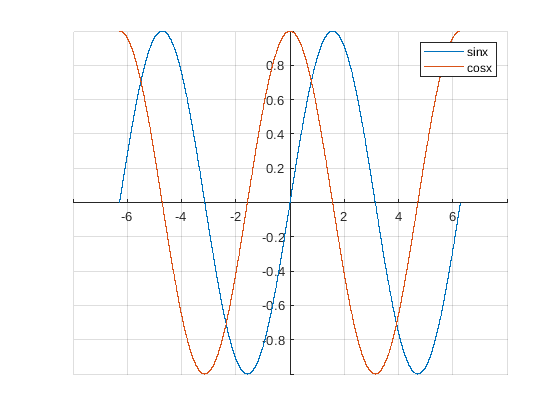
\includegraphics[width=0.5\textwidth]{Analisi1/figures/sincosx.png}
    \caption{Grafico delle funzioni $\sin x$ e $\cos x$.}
    \label{fig:sincosx}
\end{figure}

\begin{definition}[Coseno]
    La funzione
    \begin{equation*}
        \cos x\colon \mathbb R\rightarrow[-1,1]
    \end{equation*}
    rappresenta l'\gls{ascissa} di un punto $P$ (vedere Figura \ref{fig:TrigFunctionDiagram}) descritto dall'angolo $x$ sulla circonferenza goniometrica.
\end{definition}

\begin{proposition}
    Il coseno può essere rappresentato come
    \begin{equation*}
        \cos x=\frac{\overline{\rm OP}}{\overline{\rm OB}}.
    \end{equation*}
\end{proposition}

\begin{definition}[Seno]
    La funzione seno
    \begin{equation*}
        \sin x\colon \mathbb R\rightarrow[-1,1],
    \end{equation*}
    rappresenta l'\gls{ordinata} di un punto $P$ (vedere Figura \ref{fig:TrigFunctionDiagram}) descritto dall'angolo $x$ sulla circonferenza goniometrica.
\end{definition}

\begin{proposition}
    Il seno può essere rappresentato come
    \begin{equation*}
        \sin x=\frac{\overline{\rm PB}}{\overline{\rm OB}}.
    \end{equation*}
\end{proposition}

\begin{property}[Prima relazione fondamentale della goniometria]\label{def:prima_relazione_fondamentale_goniometria}
    Dato che $\sin x$ e $\cos x$ rappresentano, rispettivamente, l'ordinata e l'ascissa del punto della circonferenza goniometrica, vale la \textbf{relazione fondamentale}:
    \begin{equation}
        \cos{x}^2+\sin{x}^2 = 1.
    \end{equation}
\end{property}

\begin{definition}
    La prima relazione fondamentale della trigonometria permette di esprimere le funzioni seno e coseno come segue:
    \begin{equation}\label{eq:prima_relazione_fondamentale_goniometria}
        \begin{matrix}
            \cos^2x=1-\sin^2x,\\
            \sin^2x=1-\cos^2.
        \end{matrix}
    \end{equation}
\end{definition}

\begin{property}
    Le funzioni $\sin x$ e $\cos x$ sono periodiche di periodo $2\pi$. Questo è dovuto alla lunghezza completa della circonferenza, ovvero $2\pi$.
\end{property}

\begin{property}
    La funzione seno è dispari, la funzione coseno è pari.
\end{property}

\begin{definition}[Tangente]
    La funzione tangente è definita come
    \begin{equation*}
        \tan x=\frac{\sin x}{\cos x}\colon \mathbb R\backslash\left\{\frac{\pi}{2}+k\pi,\,k\in\mathbb Z\right\}\rightarrow\mathbb R
    \end{equation*}
    e rappresenta l'ordinata di un punto $T$ (vedere Figura \ref{fig:TrigFunctionDiagram}) descritto dall'angolo $x$ sulla circonferenza goniometrica. 
\end{definition}

I triangoli $OQP$ e $OAT$ sono simili, quindi è possibile definire la seguente proporzione
\begin{equation*}
    \underbrace{\overline{\rm AT}}_{\tan x}\colon\underbrace{\overline{\rm PQ}}_{\sin x}=\underbrace{\overline{\rm OA}}_{1}\colon\underbrace{\overline{\rm OQ}}_{\cos x}.
\end{equation*}

Pertanto, in base alla precedente proporzione è data la Definizione \ref{def:seconda_relazione_fondamentale_goniometria}.

\begin{definition}[Seconda relazione fondamentale della goniometria]\label{def:seconda_relazione_fondamentale_goniometria}
La funzione tangente è definita come
    \begin{equation}\label{eq:seconda_relazione_fondamentale_goniometria}
        \boldsymbol{\tan x=}\frac{\overline{\rm PQ}}{\overline{\rm OQ}}=\boldsymbol{\frac{\sin x}{\cos x}}.
    \end{equation}
\end{definition}

\begin{figure}
    \centering
    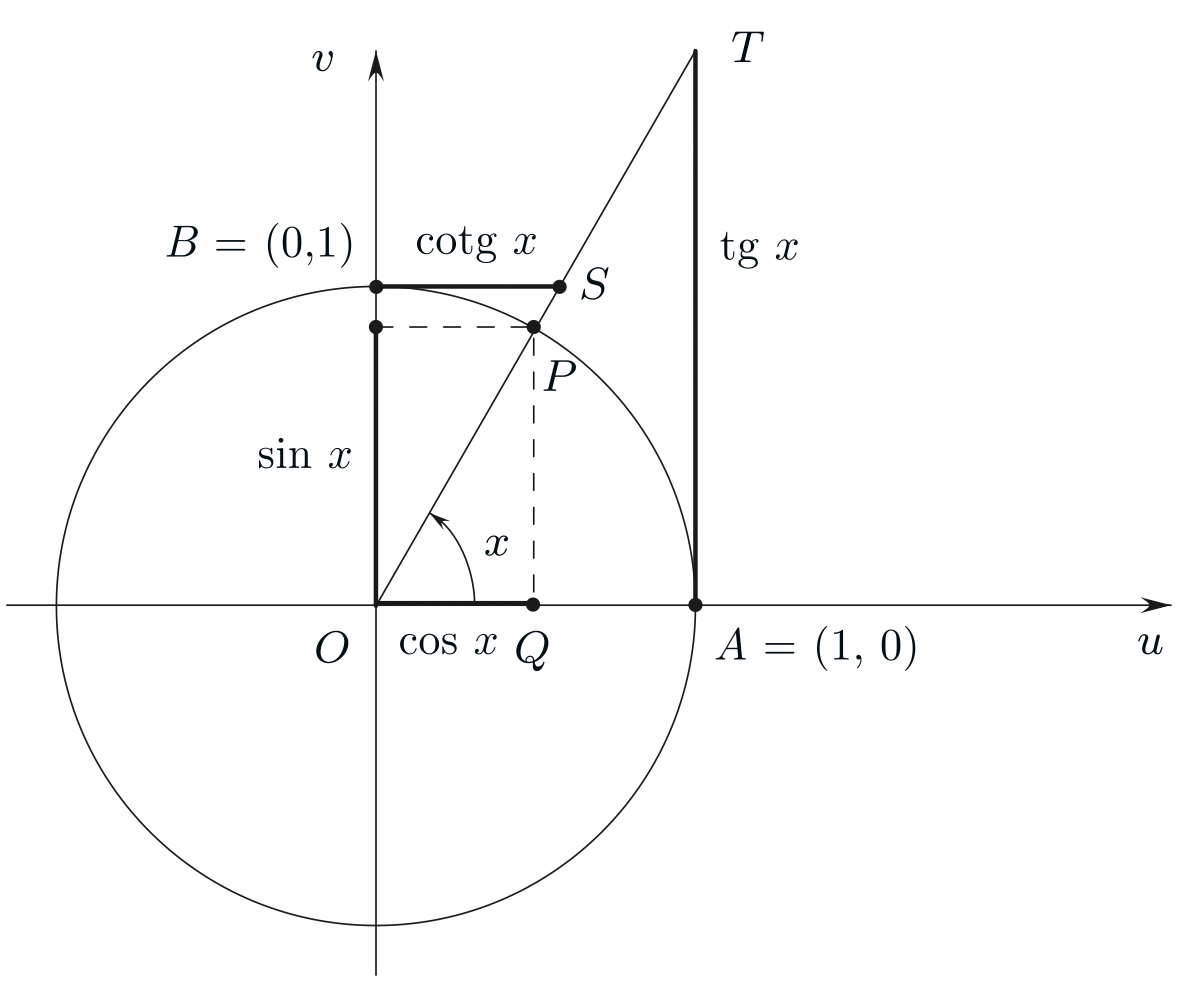
\includegraphics[width=0.5\textwidth]{Analisi1/figures/TrigFunctionDiagram.jpeg}
    \caption{Grafico delle funzioni goniometriche.}
    \label{fig:TrigFunctionDiagram}
\end{figure}

\subsubsection{Funzioni reciproche goniometriche}

\begin{definition}[Cotangente]
    La funzione
    \begin{equation*}
        \cot x = \frac{1}{\tan x}\colon\mathbb R \backslash\{0+k\pi\colon k\in\mathbb N\}\rightarrow\mathbb R
    \end{equation*}
    rappresenta l'ascissa del punto $S$ descritto dall'angolo $x$ sulla circonferenza goniometrica.
\end{definition}

\begin{property}
    La funzione cotangente è una funzione periodica di periodo $\pi$ ed è dispari. Inoltre, la cotangente è il \gls{reciproco} della funzione tangente.
\end{property}


Dato che i triangoli $OQP$ e $OSB$ sono simili, ovvero $\overline{\rm BS}\parallel\overline{\rm OQ}$ e $x'\equiv x$ è possibile definire  la proporzione
\begin{equation*}
    \overline{\rm BS}\colon\overline{\rm OQ}=\underbrace{\overline{\rm OB}}_{1}\colon\overline{\rm PQ}.
\end{equation*}

Pertanto, in base alla precedente proporzione ed alla applicazione del secondo criterio di similitudine dei triangoli \footnote{Gli angoli $x'$ e $x$ sono coincidenti perché alterni interni.} è data la Definizione \ref{def:terza_relazione_fondamentale_goniometria}.

\begin{definition}[Terza relazione fondamentale della goniometria]\label{def:terza_relazione_fondamentale_goniometria}
    La funzione cotangente è definita come
    \begin{equation*}
        \boldsymbol{\cot x=}\frac{\overline{\rm OQ}}{\overline{\rm PQ}}=\frac{1}{\tan x}=\boldsymbol{\frac{\cos x}{\sin x}}.
    \end{equation*}
\end{definition}

Con lo stesso criterio di reciprocità sono definite le seguenti funzioni.

\begin{definition}[Quarta relazione fondamentale della trigonometria]
    La funzione
    \begin{equation*}
        \boldsymbol{\sec x=\frac{1}{\cos x}}\colon\mathbb R\backslash\left\{\frac{\pi}{2}+k\pi\right\}\rightarrow\mathbb R
    \end{equation*}
    rappresenta l'ascissa di un punto $S$ (vedere Figura \ref{fig:circonferenza_goniometrica_secante}) descritto dall'angolo $x$ sulla circonferenza goniometrica.
\end{definition}

\begin{definition}[Cosecante]
    La funzione
    \begin{equation*}
        \csc x=\frac{1}{\sin x}\colon\mathbb R\backslash\left\{\frac{\pi}{2}+k\pi\right\}\rightarrow\mathbb R
    \end{equation*}
    rappresenta l'ordinata di un punto $C$ (vedere Figura \ref{fig:circonferenza_goniometrica_cosecante}) descritto dall'angolo $x$ sulla circonferenza goniometrica.
\end{definition}

\begin{figure}[!hbt]
    \centering
    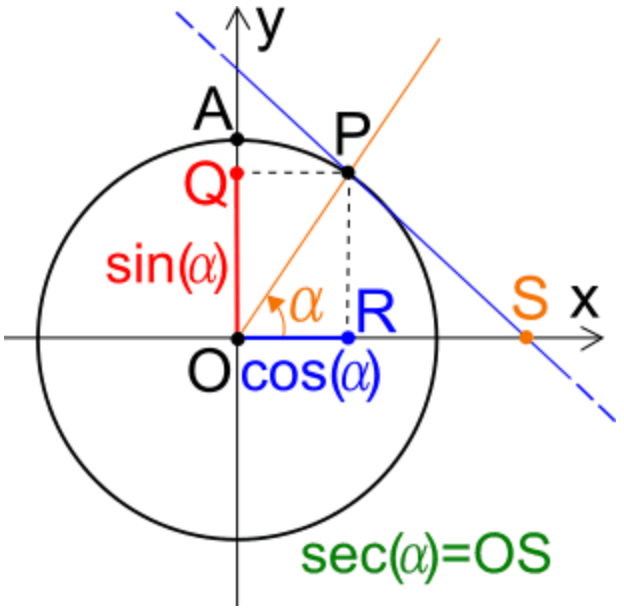
\includegraphics[width=0.5\textwidth]{Analisi1/figures/circonferenza_goniometrica_secante.jpeg}
    \caption{Grafico della funzione $\sec x$.}
    \label{fig:circonferenza_goniometrica_secante}
\end{figure}

\begin{figure}[!hbt]
    \centering
    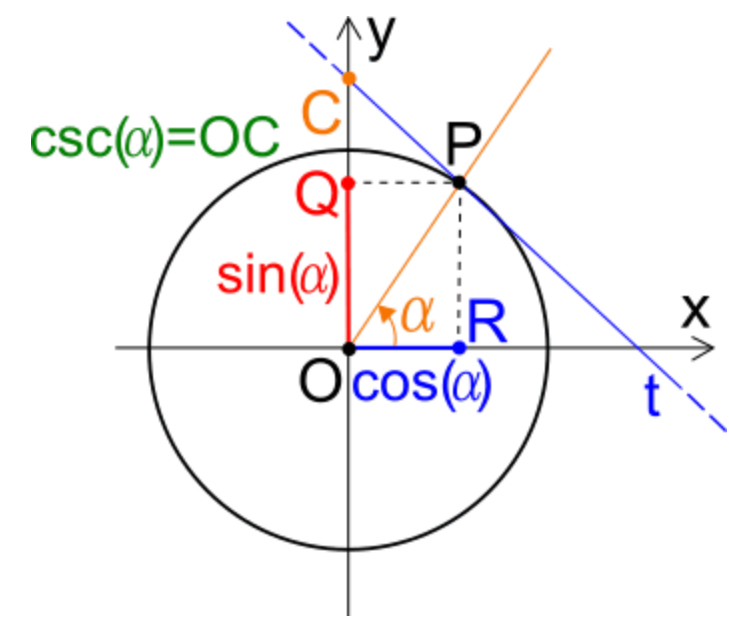
\includegraphics[width=0.5\textwidth]{Analisi1/figures/circonferenza_goniometrica_cosecante.jpeg}
    \caption{Grafico della funzione $\csc x$.}
    \label{fig:circonferenza_goniometrica_cosecante}
\end{figure}

\subsubsection{Formule goniometriche inverse}
Le funzioni gonometriche non sono invertibili, ma selezionando un tratto monotono è possibile definirne le funzioni trigonometriche inverse:

\begin{equation*}
    \arccos x\colon [-1,1]\rightarrow[0,\pi],
\end{equation*}

\begin{equation*}
    \arcsin x\colon [-1,1]\rightarrow\left[-\frac{\pi}{2},\frac{\pi}{2}\right],
\end{equation*}

\begin{equation*}
    \arctan x\colon \mathbb R\rightarrow\left(-\frac{\pi}{2},\frac{\pi}{2}\right).
\end{equation*}

\begin{definition}
    \begin{equation*}
        \begin{matrix}
            \sin(\arctan x) &=& \frac{x}{\sqrt{1+x^2}}\\\\
            \cos(\arccos x) &=& \frac{1}{\sqrt{1+x^2}}.
        \end{matrix}
    \end{equation*}
\end{definition}

\begin{property}
    Le funzioni goniometriche inverse hanno le seguenti proprietà:
    \begin{itemize}
        \item non sono funzioni goniometriche,
        \item hanno come immagine gli angoli in cui valgono le rispettive funzioni.
    \end{itemize}
\end{property}

\begin{figure}
    \centering
    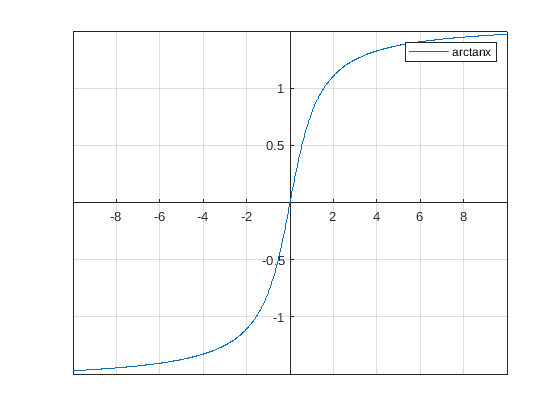
\includegraphics[width=0.5\textwidth]{Analisi1/figures/arctanx.png}
    \caption{Grafico della funzione $\arctan x$.}
    \label{fig:arctanx}
\end{figure}

\begin{figure}
    \centering
    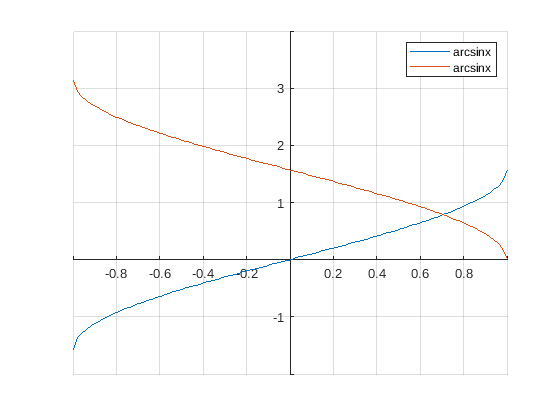
\includegraphics[width=0.5\textwidth]{Analisi1/figures/arcsincosx.png}
    \caption{Grafico delle funzioni $\arcsin x$ e $\arccos x$.}
    \label{fig:arcsincosx}
\end{figure}

\subsubsection{Archi ricorrenti}

\subsubsection{Archi associati}

\textbf{NB:} Saranno utilizzate le Figure \ref{fig:archi_associati1}-\ref{fig:archi_associati} per trattare gli archi associati.

Gli archi associati ad un angolo $\alpha$ è indicato un insieme di formule che permettono di semplificare il calcolo delle funzioni goniometriche.

\begin{definition}
    Dato un angolo $\alpha$, formule sono associate sono definite per i seguenti: $\frac{\pi}{2}\pm\alpha,\, \pi \pm \alpha,\, \frac{3}{2}\pi\pm\alpha,\, 2\pi - \alpha$.
\end{definition}

\paragraph{Osservazioni suFigura \ref{fig:archi_associati1}:} È possibile osservare che:
\begin{itemize}
    \item Il punto $P''$ è il simmetrico di $P$ rispetto all'asse $y$.
    \item Il punto $P^{iv}$ è simmetrico di $P$ rispetto all'asse $x$.
    \item Il punto $P'''$ è il simmetrico di $P$ rispetto all'origine.
\end{itemize}

\begin{figure}
    \centering
    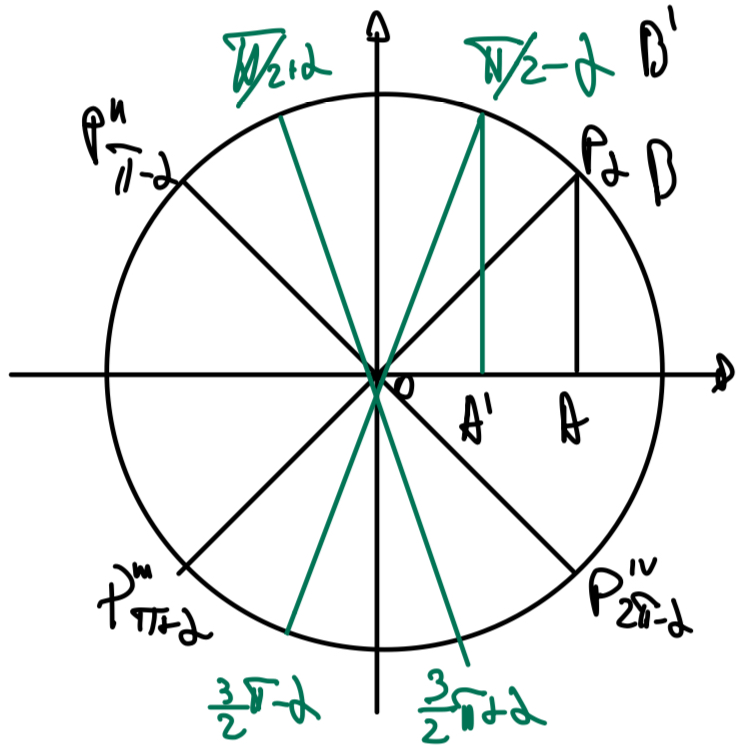
\includegraphics[width=0.5\textwidth]{Analisi1/figures/archi_associati1.jpeg}
    \caption{Archi associati}
    \label{fig:archi_associati1}
\end{figure}

\begin{figure}
    \centering
    
\includegraphics[width=0.5\textwidth]{Analisi1/figures/archi_associati.png}
    \caption{Archi associati}
    \label{fig:archi_associati}
\end{figure}

\paragraph{Angoli opposti e supplementari}
\begin{definition}[Angolo opposto]
    L'angolo opposto di $\alpha$ è $-\alpha$.
\end{definition}

\begin{definition}[Angolo esplementare]
    L'angolo esplementare di $\alpha$ è un angolo che sommato ad $\alpha$ è uguale a $2\pi$.
\end{definition}

Angolo esplementare ed angolo opposto coincidono nel contesto della circonferenza goniometrica in quanto $-\alpha=(0-\alpha)=2\pi-\alpha$.

\begin{definition}[Archi associati per $\alpha$]
    \begin{equation*}
        \begin{matrix}
            \sin(-\alpha)&=&-\sin\alpha,\\
            \cos(-\alpha)&=&\cos(\alpha),\\
            \tan(-\alpha)&=&-\tan(\alpha),\\
            \cot(-\alpha)&=&-\cot(\alpha).
        \end{matrix}
    \end{equation*}
\end{definition}

\paragraph{Archi supplementari}
\begin{definition}[Archi associati per $\pi-\alpha$]
    \begin{equation*}
        \begin{matrix}
            \sin(\pi-\alpha)&=&\sin(\alpha),\\
            \cos(\pi-\alpha)&=&-\cos(\alpha),\\
            \tan(\pi-\alpha)&=&-\tan(\alpha),\\
            \cot(\pi-\alpha)&=&-\cot(\alpha).
        \end{matrix}
    \end{equation*}
\end{definition}

\begin{definition}[Archi associati $\pi+\alpha$]
    \begin{equation*}
        \begin{matrix}
            \sin(\pi+\alpha)&=&-\sin(\alpha),\\
            \cos(\pi+\alpha)&=&-\cos(\alpha),\\
            \tan(\pi+\alpha)&=&\tan(\alpha),\\
            \cot(\pi+\alpha)&=&\cot(\alpha).
        \end{matrix}
    \end{equation*}
\end{definition}

\paragraph{Angoli complementari}

\begin{definition}[Archi associati $\frac{\pi}{2}-\alpha$]
    \begin{equation*}
        \begin{matrix}
            \sin\left(\frac{\pi}{2}-\alpha\right)&& &=& &&\cos(\alpha),\\
            \cos\left(\frac{\pi}{2}-\alpha\right)&& &=& &&\sin(\alpha),\\
            \tan\left(\frac{\pi}{2}-\alpha\right)&=&\frac{\sin\left(\pi-\alpha\right)}{\cos\left(\pi-\alpha\right)}&=&\frac{\cos(\alpha)}{\sin(\alpha)}&=&\cot(\alpha)\\
            \cot\left(\frac{\pi}{2}-\alpha\right)&=&\frac{\cos(\pi-\alpha)}{\sin(\pi-\alpha)}&&&=&\tan\alpha.
        \end{matrix}
    \end{equation*}
\end{definition}

Le precedenti formule sono dovute al fatto che $B'$ e $B$ sono congruenti ed i triangoli $OAB$ e $OA'B'$ siano simili (sono lo stesso traslato in quanto $\overline{\rm A'B'}=\overline{\rm OA}$ e $\overline{\rm OA}=\overline{\rm AB}$).

Traslando il triangolo $OA'B'$ nel secondo quadrante è ottenuto quanto segue.

\begin{definition}[Archi associati $\frac{\pi}{2}+\alpha$]
    \begin{equation*}
        \begin{matrix}
            \sin\left(\frac{\pi}{2}+\alpha\right)&& &=& &&\cos(\alpha),\\
            \cos\left(\frac{\pi}{2}+\alpha\right)&& &=& &&-\sin(\alpha),\\
            \tan\left(\frac{\pi}{2}+\alpha\right)&=&\frac{\sin\left(\pi+\alpha\right)}{\cos\left(\pi+\alpha\right)}&=&\frac{\cos(\alpha)}{-\sin(\alpha)}&=&-\cot(\alpha),\\
            \cot\left(\frac{\pi}{2}+\alpha\right)&=&\frac{\cos(\pi+\alpha)}{\sin(\pi+\alpha)}&&&=&-\tan\alpha.
        \end{matrix}
    \end{equation*}
\end{definition}

Traslando i quadranti sono ottenute le seguenti definizione.

\begin{definition}[Archi associati per $\frac{3\pi}{2}-\alpha$]
    \begin{equation*}
        \begin{matrix}
            \sin\left(\frac{3\pi}{2}-\alpha\right)&\overset{\frac{3\pi}{2}=-\frac{\pi}{2}}{=}& \sin\left(-\frac{\pi}{2}-\alpha\right)&=&\sin\left[-\left(\frac{\pi}{2}+\alpha\right)\right]\overset{\footnotemark}{=}-\cos\alpha,\\
            \cos\left(\frac{3\pi}{2}-\alpha\right)&=&&=&-\sin\alpha,\\
            \tan\left(\frac{3\pi}{2}-\alpha\right)&=& &=&\cot\alpha,\\
            \cot\left(\frac{3\pi}{2}-\alpha\right)&=&&=&\tan\alpha.
        \end{matrix}
    \end{equation*}
\end{definition}
\footnotetext{$\sin(-\alpha)=-\sin\alpha$.}

\begin{definition}[Archi associati per $\frac{3\pi}{2}+\alpha$]
    \begin{equation*}
        \begin{matrix}
            \sin\left(\frac{3\pi}{2}+\alpha\right)&\overset{\frac{3\pi}{2}=-\frac{\pi}{2}}{=}& \sin\left(-\frac{\pi}{2}+\alpha\right)&=&\sin\left[-\left(\frac{\pi}{2}-\alpha\right)\right]&\overset{\footnotemark}{=}&-\cos\alpha,\\
            \cos\left(\frac{3\pi}{2}+\alpha\right)&=&&=&\sin\alpha,\\
            \tan\left(\frac{3\pi}{2}+\alpha\right)&=& &=&-\cot\alpha,\\
            \cot\left(\frac{3\pi}{2}+\alpha\right)&=&&=&-\tan\alpha.
        \end{matrix}
    \end{equation*}
\end{definition}

\subsubsection{Formule parametriche del seno e coseno}
Le formule parametriche permettono di esprimere il seno ed il cose in funzione di $\tan\left(\frac{\alpha}{2}\right)$ e sono utili anche per il calcolo integrale.
\begin{definition}[Formula parametrica di $\sin x$]
    \begin{equation}\label{eq:formula_parametrica_seno}
        \begin{matrix}
            \boldsymbol{\sin\alpha}&\boldsymbol =& \sin\left[2\left(\frac{\alpha}{2}\right)\right] &\overset{\ref{eq:formula_duplicazione_seno}}{=}& 2\sin\frac{\alpha}{2}\cos\frac{\alpha}{2}&\equiv&\frac{2\sin\frac{\alpha}{2}\cos\frac{\alpha}{2}}{1}&\overset{(\ref{eq:prima_relazione_fondamentale_goniometria})}{=}&\frac{2\sin\frac{\alpha}{2}\cos\frac{\alpha}{2}}{\underbrace{\sin^2\frac{\alpha}{2}+\cos^2\frac{\alpha}{2}}_{\footnotemark}} \\
            && &\overset{\footnotemark}{=}& \frac{\frac{2\sin\frac{\alpha}{2}\cancel{\cos\frac{\alpha}{2}}}{\cos^{\cancel{2}}\frac{\alpha}{2}}}{\underbrace{\frac{\sin^2\frac{\alpha}{2}+\cos^2\frac{\alpha}{2}}{\cos^2\frac{\alpha}{2}}}_{\footnotemark}}&=& \frac{\frac{2\sin\frac{\alpha}{2}}{\cos\frac{\alpha}{2}}}{\frac{\sin^2\frac{\alpha}{2}}{\cos^2\frac{\alpha}{2}}+\frac{\cancel{\cos^2\frac{\alpha}{2}}}{\cancel{\cos^2\frac{\alpha}{2}}}}&=& \boldsymbol{\frac{2\tan\frac{\alpha}{2}}{\tan^2\frac{\alpha}{2}+1}}
        \end{matrix}
    \end{equation}
\end{definition}

\begin{definition}[Formula parametrica di $\cos x$]
    \begin{equation}\label{eq:formula_parametrica_coseno}
        \begin{matrix}
            \boldsymbol{\cos\alpha} &=& \cos\left[2\left(\frac{\alpha}{2}\right)\right] &=& \cos^2\frac{\alpha}{2}-\sin^2\frac{\alpha}{2} &\equiv& \frac{\cos^2\frac{\alpha}{2}-\sin^2\frac{\alpha}{2}}{1} \\\\
            && &=& \frac{\cos^2\frac{\alpha}{2}-\sin^2\frac{\alpha}{2}}{\sin^2\frac{\alpha}{2}+\cos^2\frac{\alpha}{2}} &=& \frac{\frac{\cos^2\frac{\alpha}{2}-\sin^2\frac{\alpha}{2}}{\cos^2\frac{\alpha}{2}}}{\frac{\sin^2\frac{\alpha}{2}+\cos^2\frac{\alpha}{2}}{\cos^2\frac{\alpha}{2}}}&=&\boldsymbol{\frac{1-\tan^2\frac{\alpha}{2}}{1+\tan^2\frac{\alpha}{2}}}
        \end{matrix}
    \end{equation}
\end{definition}

\addtocounter{footnote}{-2}
\footnotetext{L'angolo della prima relazione fondamentale della goniometria (\ref{eq:prima_relazione_fondamentale_goniometria}) può essere qualsiasi, quindi è scelto $\frac{\alpha}{2}$.}

\stepcounter{footnote}
\footnotetext{Moltiplicazione e divisione per $\cos^2\frac{\alpha}{2}$ con la condizione che $\cos^2\frac{\alpha}{2}\neq 0$. La condizione si verifica se $\alpha\neq\frac{\pi}{2}+k\pi$, quindi se $\alpha\neq\pi$.}

\stepcounter{footnote}
\footnotetext{Proprietà distributiva della divisione.}

Le formule (\ref{eq:formula_parametrica_seno}) e (\ref{eq:formula_parametrica_coseno}) possono essere considerate, utilizzando l'uguaglianza
\begin{equation*}
    \tan\frac{\alpha}{2}=t,
\end{equation*}

come segue
\begin{equation*}
    \begin{matrix}
        \sin\alpha &=& \frac{2t}{t^2+1},\\
        \\
        \cos\alpha &=& \frac{1-t^2}{1+t^2}.
    \end{matrix}
\end{equation*}

\subsubsection{Formule di addizione e sottrazione}
\begin{definition}[Formula addizione e sottrazione $\sin x$]
    \begin{equation}\label{eq:addizione_sottrazione_seno}
        \sin(\alpha\pm\beta)=\sin\alpha\cos\beta\pm\sin\beta\cos\alpha.
    \end{equation}
\end{definition}

\begin{definition}[Formula addizione e sottrazione $\cos x$]
    \begin{equation}\label{eq:addizione_sottrazione_coseno}
        \cos(\alpha\pm\beta)=\cos\alpha\cos\beta\mp\sin\alpha\sin\beta.
    \end{equation}
\end{definition}

\begin{definition}[Formula addizione e sottrazione $\tan x$]
    \begin{equation}\label{eq:addizione_sottrazione_tangente}
        \tan(\alpha\pm\beta)=\frac{\tan\alpha+\tan\beta}{1\mp\tan\alpha\tan\beta}.
    \end{equation}
\end{definition}

\paragraph{Intermezzo passaggi $\boldsymbol{\tan(\alpha\pm\beta)=\frac{\tan\alpha+\tan\beta}{1\mp\tan\alpha\tan\beta}}$:}
\begin{equation*}
    \begin{matrix}
        \boldsymbol{\tan(\alpha+\beta)}&\overset{(\ref{eq:seconda_relazione_fondamentale_goniometria})}{=}&\frac{\sin(\alpha+\beta)}{\underbrace{\cos(\alpha+\beta)}_{\footnotemark}}&\overset{(\ref{eq:addizione_sottrazione_seno})-(\ref{eq:addizione_sottrazione_coseno})}{=}&\frac{\sin\alpha\cos\beta+\sin\beta\cos\alpha}{\cos\alpha\cos\beta-\sin\alpha\sin\beta}\\
        &\overset{\footnotemark}{=}&\frac{\frac{\sin\alpha\cos\beta}{\cos\alpha\cos\beta}+\frac{\cos\alpha\cos\beta}{\cos\alpha\cos\beta}}{\frac{\cos\alpha\cos\beta}{\cos\alpha\cos\beta}-\frac{\sin\alpha\sin\beta}{\cos\alpha\cos\beta}}&=&\frac{\frac{\sin\alpha}{\cos\alpha}+\frac{\sin\beta}{\cos\beta}}{1-\frac{\sin\alpha}{\cos\beta}\frac{\sin\beta}{\cos\beta}}&=&\boldsymbol{\frac{\tan\alpha+\tan\beta}{1-\tan\alpha\tan\beta}},
    \end{matrix}
\end{equation*}

\addtocounter{footnote}{-1}
\footnotetext{La condizione è che $\cos(\alpha-\beta)$, ovvero $\alpha+\beta\neq\frac{\pi}{2}+k\pi$.}

\stepcounter{footnote}
\footnotetext{Divisione per $\cos\alpha\cos\beta$, supponendo $\alpha\neq\frac{\pi}{2}+k'\pi$ e $\beta\neq\frac{\pi}{2}+k''\pi$.}

\begin{equation*}
    \tan(\alpha-\beta)=\tan(\alpha+(-\beta))=\frac{\tan\alpha+\tan(-\beta)}{1-\tan\alpha\tan\beta}=\frac{\tan\alpha+\tan\beta}{1+\tan\alpha\tan\beta}.
\end{equation*}

\begin{example}
    $\sin(15^\circ)=\sin(\frac{\pi}{4}-\frac{\pi}{6})=\sin\frac{\pi}{4}\cos\frac{\pi}{6}-\sin\frac{\pi}{6}\cos\frac{\pi}{4}=\frac{\sqrt{6}-\sqrt{2}}{4}=\frac{\sqrt{2}}{2}\cdot-\frac{1}{2}\cdot\frac{\sqrt{2}}{2}$.
\end{example}

\begin{remark}
    Le formule degli archi associati sono casi particolari delle formule precedenti.
\end{remark}

\begin{example}
    $\sin(\pi-\alpha)=\underbrace{\sin\pi}_{0}\cos\alpha-\sin\alpha\underbrace{\cos\pi}_{-1}=\sin\alpha$.
\end{example}


\subsubsection{Formule di duplicazione}
Le formule i duplicazione sono casi particolari delle formule di addizione e sottrazione.

\begin{definition}[Formula duplicazione $\sin x$]
    \begin{equation}\label{eq:formula_duplicazione_seno}
        \sin(2\alpha)=\sin(\alpha+\alpha)=2\sin\alpha\cos\alpha.
    \end{equation}
\end{definition}

\begin{definition}[Formula duplicazione $\cos x$]\label{def:formula_duplicazione_coseno}
    \begin{equation}\label{eq:formula_duplciazione_coseno}
        \cos(2\alpha)=\cos(\alpha+\alpha)=\cos^2\alpha-\sin^2\alpha\overset{(\ref{eq:prima_relazione_fondamentale_goniometria})}{=}
        \begin{cases}
            2\cos^2\alpha-1,\\
            1-2\sin^2\alpha.
        \end{cases}
    \end{equation}
\end{definition}

\begin{definition}[Formula duplicazione $\tan x$]
    \begin{equation*}
        \tan(2\alpha)=\tan(\alpha+\alpha)=\frac{\tan\alpha+\tan\alpha}{1-\tan\alpha\tan\alpha}=\frac{2\tan\alpha}{1-\tan\alpha}.
    \end{equation*}
\end{definition}

E' possibile utilizzare la formula di duplicazione del coseno per esprimere in modo diverso $\sin^2\alpha$ e $\cos^2\alpha$.
\begin{remark}
    Sia, dalla Definizione \ref{def:formula_duplicazione_coseno}, $\cos(2\alpha)=1-\sin^2\alpha$ allora
    \begin{equation}
        \begin{matrix}
            \sin^2\alpha=\frac{1-\cos(2\alpha)}{2}\rightarrow\sin\alpha=\pm\sqrt{\frac{1-\cos(2\alpha)}{2}}\\
            \cos^2\alpha=\frac{1+\cos(2\alpha)}{2}\rightarrow\cos\alpha=\pm\sqrt{\frac{1-\cos(2\alpha)}{2}}
        \end{matrix}
    \end{equation}
\end{remark}

\subsubsection{Formule di prostaferesi}
Le formule di prostaferesi sono formule goniometriche che consentono di trasformare la somma e la differenza di due seni o di due coseni in un prodotto tra seno e coseno.
\begin{definition}[Per il seno]
    \begin{equation*}
        \begin{matrix}
            \sin(\alpha)+\sin(\beta) &=& 2 \sin\left(\frac{\alpha+\beta}{2}\right)\cdot\cos \left(\frac{\alpha-\beta}{2}\right)\\
            \sin(\alpha)-\sin(\beta) &=& 2 \cos\left(\frac{\alpha+\beta}{2}\right)\cdot\sin \left(\frac{\alpha-\beta}{2}\right)
        \end{matrix}
    \end{equation*}
\end{definition}

\begin{definition}[Per il coseno]
    \begin{equation*}
        \begin{matrix}
            \cos\alpha+\cos\beta &=& 2\cos\left(\frac{\alpha+\beta}{2}\right)\cos\left(\frac{\alpha -\beta}{2}\right)\\
            \cos\alpha-\cos\beta &=& -2\sin\left(\frac{\alpha+\beta}{2}\right)\sin\left(\frac{\alpha -\beta}{2}\right)
        \end{matrix}
    \end{equation*}
\end{definition}

\subsubsection{Formule di bisezione}
Le formule di bisezione sono ricavate dalla formula di duplicazione del seno sostituendo $\alpha$ con $\frac{\alpha}{2}$.

\begin{definition}
    \begin{equation*}
        \begin{matrix}
            \sin\left(\frac{\alpha}{2}\right)&=&\pm\sqrt{\frac{1-\cos\alpha}{2}},\\
            \cos\left(\frac{\alpha}{2}\right)&=&\pm\sqrt{\frac{1+\cos\alpha}{2}},
        \end{matrix}
    \end{equation*}
    \begin{equation*}
        \tan\left(\frac{\alpha}{2}\right)=\frac{\sin\frac{\alpha}{2}}{\frac{\cos\alpha}{2}}=\frac{\pm\sqrt{\frac{\-\cos\alpha}{2}}}{\pm\sqrt{\frac{1+\cos\alpha}{2}}}=\pm\sqrt{\frac{1-\cos\alpha}{1+\cos\alpha}}.
    \end{equation*}
\end{definition}

\subsubsection{Formule di Werner}
Le formule di Werner sono ricavate sommando membro a membro le formule di addizione.

\begin{definition}
    \begin{equation*}
        \begin{matrix}
            \sin\alpha\sin\beta &=& \frac{1}{2}[\cos(\alpha-\beta)-\cos(\alpha+\beta)],\\\\
            \cos\alpha\cos\beta &=& \frac{1}{2}[\cos(\alpha+\beta)+\cos(\alpha-\beta)],\\\\
            \sin\alpha\cos\beta &=& \frac{1}{2}[\sin(\alpha+\beta)+\sin(\alpha-\beta)].
        \end{matrix}
    \end{equation*}
\end{definition}

\section{Successioni Numeriche}
\begin{definition}[Successione]
    Una successione e' una funzione indicata come
    \begin{equation*}
        \{a_n\}_{n\in\mathbb N}\colon\mathbb N\rightarrow\mathbb R,
    \end{equation*}
    dove $a_n$ e' il numero reale associato all'intero $n$.
\end{definition}

\begin{remark}
    Per una successione $\{a_n\}_{n\in\mathbb N}$ sono valide le Definizioni \ref{def:funzione_crescente}-\ref{def:funzione_monotona} di funzione crescente, strettamente crescente e monotona.
\end{remark}

Siano definite le seguenti successioni, per $n\in\mathbb N$:
\begin{equation*}
    \begin{matrix}
        \Tilde{a}_n=\frac{1}{n} & b_n = n^2 & c_n = \frac{1-(-1)^n}{2}\\
        &&\\
        d_n=|\{d\in\mathbb R\colon d|n\}| & e_n=\sum_{k=1}^n\frac{3}{10^k} & f_n=\frac{n}{2}\sin\frac{2\pi}{n}\\
        &&\\
        g_n= \frac{n}{n+1} & h_n=n! & i_n= (-1)^n\\
        &&\\
        j_n=\frac{(-1)^n}{n} &  & l_n = (-1)^n n
    \end{matrix}
\end{equation*}

\begin{remark}
    $b_n,\, e_n,\, f_n,\, g_n,$ e $h_n$ sono strettamente crescenti. $\Tilde{a}_n$ e' strettamente descrente. $c_n\, d_n$ e $j_n$ non sono monotone.
\end{remark}

\begin{definition}[Successione limitata]
    Una successione $\{a_n\}_{n\in\mathbb N}$ e' limitata se esistono $m$ e $M$ tali che
    \begin{equation*}
        m\leq a_n\leq M,\quad \forall n\in\mathbb N.
    \end{equation*}
\end{definition}

Cosi' anche se esiste $M>0$ tale che
\begin{equation*}
    |a_n|\leq M,\quad \forall n\in\mathbb N.
\end{equation*}

\begin{definition}[Sottosucessione]\label{def:sottosuccessione}
    Sia $\{a_n\}$ una successione. Diciamo che $\{a_{n_k}\}$ e' una
    sottosuccessione di $\{a_n\}$ se la successione di numeri naturali
    \begin{equation*}
        \begin{aligned}
            \mathbb N &\rightarrow\mathbb N\\
            k &\mapsto n_k
        \end{aligned}
    \end{equation*}
    e' strettamente crescente
\end{definition}

\subsection{Successioni convergenti}
\begin{definition}[Successione convergente]
    Sia $L\in\mathbb R$. La successione $\{a_n\}_{n\in\mathbb N}$ converge a $L$, ovvero
    \begin{equation*}
        \lim_{n\rightarrow+\infty}a_n=L,
    \end{equation*}
    se per ogni $\varepsilon>0$ esiste $n_\varepsilon$ tale che
    \begin{equation}\label{eq:accuratezza_limite_successione_convergente}
        |a_n-L|<\varepsilon,\,\forall n>n_\varepsilon.
    \end{equation}
\end{definition}

\begin{remark}\label{rem:successione_convergente_limitata}
    La condizione (\ref{eq:accuratezza_limite_successione_convergente}) equivale a
    \begin{equation*}
        L-\varepsilon < a_n < L+\varepsilon,
    \end{equation*}
    ovvero
    \begin{equation*}
        a_n\in(L-\varepsilon,L+\varepsilon).
    \end{equation*}
\end{remark}

\begin{definition}[Successione infinitesima]
    Una successione è detta infinitesima se tende a 0.
\end{definition}

\begin{proposition}
    La successione $a_n$ è infinitesima se e solo se $|a_n|$ è infinitesima.
\end{proposition}
\begin{proof}
    Pagina 35.
\end{proof}

\begin{example}       $\lim_{n\rightarrow+\infty}\Tilde{a} = 0$
\end{example}

\begin{example}
    $\lim_{n\rightarrow+\infty}j_n = 0.$
\end{example}

\begin{example}
    $\lim_{n\rightarrow+\infty}e_n = \frac{1}{3}.$
\end{example}

\begin{example}
    $\lim_{n\rightarrow+\infty}g_n = 1.$
\end{example}

\begin{theorem}[Unicita' del limite]
    Una successione convergente non puo' avere due limiti distinti.
\end{theorem}
\begin{proof}
    Vedere pagina 29.
\end{proof}

\begin{example}[Successione non convegente]
    La successione $c_n$ vale alternativamente 0 oppure 1, quindi non potrà essere contenuta in un raggio minore di $\frac{1}{2}$. Lo stesso $i_n$.
\end{example}

\begin{theorem}\label{th:successione_convergente_limitata}
    Ogni successione convergente e' limitata.
\end{theorem}
\begin{proof}
    Vedere pagina 30.
\end{proof}

\begin{remark}
    Il Teorema \ref{th:successione_convergente_limitata} afferma che la "limitazione" e' una condizione necessaria ma non sufficiente, quindi non afferma che una successione limitata e' convergente.
\end{remark}

\begin{example}[Successioni non convergenti]
    Le successioni $b_n,\, d_n$ e $h_n$ non sono limitate quindi non possono essere convergenti. Le successioni $c_n$ ed $i_n$ sono limitate ma non convergenti.
\end{example}


\begin{proposition}
    Data ${a_n}_{n\in\mathbb N}$, se e' convergente allora ha le seguenti proprieta':
    \begin{enumerate}
        \item \textbf{Unicita':} ${a_n}_{n\in\mathbb N}$ ha al piu' un limite,
        \item \textbf{Limitatezza:} Osservazione \ref{rem:successione_convergente_limitata},
        \item \textbf{Sottinsieme convergente:} Ogni sottoinsieme di ${a_n}_{n\in\mathbb N}$ converge allo stesso limite di ${a_n}_{n\in\mathbb N}$.
    \end{enumerate}
\end{proposition}

\subsubsection{Operazioni con i limiti}

\begin{proposition}
    Se $\lim_{n\rightarrow+\infty}a_n=a$ e $\lim_{n\rightarrow+\infty}b_n=b$, per ogni $a,b\in\mathbb R$ allora:
    \begin{itemize}
        \item $\lim_{n\rightarrow+\infty}(\alpha a_n+\beta b_n)=\alpha a_n+\beta b_n,\quad \forall\alpha ,\,\beta\in\mathbb R,$
        \item $\lim_{n\rightarrow+\infty}(a_n\cdot b_n)=a\cdot b,$
        \item $\lim_{n\rightarrow+\infty}\frac{a_n}{b_n}=\frac{a}{b}\quad \text{ se } b\neq 0.$
    \end{itemize}
\end{proposition}

\begin{proposition}
    Il prodotto tra una successione infinitesima e limitata è una successione infinitesima.
\end{proposition}

\subsection{Successioni divergenti ed indeterminate}
\begin{definition}\label{def:successione_divergente}[Successione divergente]
    La successione $\{a_n\}_{n\in\mathbb N}$ diverge a $+\infty$, ovvero
    \begin{equation*}
        \lim_{n\rightarrow+\infty}a_n=+\infty,
    \end{equation*}
    se per ogni $M>0$ esiste $n_M$ tale che $a_n>M$ per ogni $n>n_M$.\\
    La successione $\{a_n\}_{n\in\mathbb N}$ diverge a $-\infty$, ovvero
    \begin{equation*}
        \lim_{n\rightarrow+\infty}a_n=-\infty,
    \end{equation*}
    se per ogni $M>0$ esiste $n_M$ tale che $a_n<-M$ per ogni $n>n_M$.    
\end{definition}

$n_M$ è da considerare come numero naturale oltre il quale ogni valore assunto dalla successione è maggiore di $M$.

\begin{example}[Successioni divergenti]
    $b_n$ e $h_n$ divergono a $+\infty$.
\end{example}

\paragraph{N.B.:}\textbf{Una successione ha limite se e' convergente oppure divergente.}

\begin{definition}[Successione indeterminata]
    Una successione che non e' divergente o convergente e' detta indeterminata (non ha limite).
\end{definition}

\begin{example}[Successioni indeterminate]
    $d_n$ ed $l_n$ sono indeterminate. $l_n$ e' illimitata superiormente ed inferiormente, non diverge perche' assume infinite volte, in modo alternato, valori positivi e negativi.
\end{example}

\begin{remark}\label{re:successione_divergente_illimitata}
    Dalla Definizione \ref{def:successione_divergente} di Successione divergente e' possibile osservare che ogni successione divergente e' illimitata.
\end{remark}

\subsubsection{Operazioni con i limiti}
Per le operazioni tra successioni divergenti valgono le seguenti proprieta'.
\begin{property}[Somma di successioni]
    Vedere Tabella \ref{tab:somma_successioni_divergenti}.
    \begin{table}[!hbt]
        \centering
        \begin{tabular}{|c|c|c|}
            \hline
            $a_n\rightarrow a\in\mathbb R$ & $b_n\rightarrow\pm\infty$ & $a_n+b_n = \pm\infty$\\
            \hline
            $a_n \rightarrow\pm\infty$ & $b_n\rightarrow\pm\infty$ & $a_n+b_n\rightarrow\pm\infty$\\
            \hline
        \end{tabular}
        \caption{Somma di successioni divergenti}
        \label{tab:somma_successioni_divergenti}
    \end{table}
\end{property}

\begin{property}[Prodotto di successioni]
    Vedere Tabella \ref{tab:prodotto_successioni_divergenti}.
    \begin{table}[!hbt]
        \centering
        \begin{tabular}{|c|c|c|}
            \hline
            $a_n\rightarrow a\neq 0$ & $b_n\rightarrow\pm\infty$ & $a_nb_n = \pm(sgn(a))\infty$\\
            \hline
            $a_n \rightarrow\pm\infty$ & $b_n\rightarrow\pm\infty$ & $a_n+b_n\rightarrow+\infty$\\
            \hline
            $a_n \rightarrow\mp\infty$ & $b_n\rightarrow\pm\infty$ & $a_n+b_n\rightarrow-\infty$\\
            \hline
        \end{tabular}
        \caption{Prodotto di successioni divergenti}
        \label{tab:prodotto_successioni_divergenti}
    \end{table}
\end{property}

\begin{property}[Rapporto di successioni]
    Vedere Tabella \ref{tab:rapporto_successioni_divergenti}.
    \begin{table}[!hbt]
        \centering
        \begin{tabular}{|c|c|c|}
            \hline
            $a_n\rightarrow a\in\mathbb R$ & $b_n\rightarrow\pm\infty$ & $\frac{a_n}{b_n}=0$\\
            \hline
            $a_n \rightarrow\pm\infty$ & $b_n\rightarrow b\neq 0$ & $\frac{a_n}{b_n}\rightarrow \pm(sgn(b))\infty$\\
            \hline
        \end{tabular}
        \caption{Rapporto di successioni divergenti}
        \label{tab:rapporto_successioni_divergenti}
    \end{table}
\end{property}

\begin{property}[Rapporto di Successioni con Successioni infinitesime]
    Vedere Tabella \ref{tab:proprieta_successioni_divergenti}.
    \begin{table}[!hbt]
        \centering
        \begin{tabular}{|c|c|c|}
            \hline
            $a_n\rightarrow a\neq 0$ & $b_n\rightarrow 0$ & $\frac{a_n}{b_n} = +\infty$\\
            \hline
            $a_n \rightarrow\pm\infty$ & $b_n\rightarrow 0$ & $\frac{a_n}{b_n} = +\infty$\\
            \hline
        \end{tabular}
        \caption{Somma di Successioni divergenti}
        \label{tab:proprieta_successioni_divergenti}
    \end{table}
\end{property}

\begin{remark}
    Anche nel caso della Tabella \ref{tab:proprieta_successioni_divergenti} la successione $\frac{a_n}{b_n}$ potrebbe non avere limite. Vedere il caso $a_n=1,\, b_n=\frac{(-1)^n}{n}$.
\end{remark}

\subsection{Confronto fra successioni}
\begin{theorem}[Teorema della permanenza del segno]
    La successione $a_n$ è definitivamente positiva se
    \begin{equation*}
        \lim_{n\rightarrow +\infty}a_n=a>0.
    \end{equation*}
\end{theorem}
\begin{proof}
    Pagina 32.
\end{proof}

Se la successione converge ad un numero negativo allora è definitivamente negativa.

\begin{corollary}
    Se $a_n\geq 0,\,\forall n\in\mathbb N$ e $\lim_{n\rightarrow +\infty}a_n=a$, allora $a\geq 0$.
\end{corollary}

\begin{remark}
    Se la successione $a_n$ è sempre positiva, non è possibile concludere che il limite è strettamente positivo. Un esempio è $a_n=\frac{1}{n}$.
\end{remark}

\begin{corollary}[Confronto per successioni convergenti]
    Se $a_n\leq b_n,\,\forall n\in\mathbb N$ e $\lim_{n\rightarrow\infty}a_n=a,\, \lim_{n\rightarrow\infty}b_n=b$, allora $a\leq b$.
\end{corollary}

\begin{theorem}[Teorema dei due carabinieri]
    Siano $a_n,b_n,c_n$ successioni tali che
    \begin{equation*}
        a_n\leq b_n\leq c_n,\,\forall n\in\mathbb N.
    \end{equation*}
    Se
    \begin{equation*}
        \lim_{n\rightarrow+\infty}a_n=\lim_{n\rightarrow+\infty}c_n=P\in\mathbb R,
    \end{equation*}
    allora
    \begin{equation*}
        \lim_{n\rightarrow+\infty}c_n=P.
    \end{equation*}
\end{theorem}
\begin{proof}
    Pagina 33.
\end{proof}

\begin{remark}
    Le successioni $a_n$ e $c_n$ devono convergere allo stesso limite.
\end{remark}

\begin{example}
    Da
    \begin{equation*}
        0\leq \frac{n^2}{n^3+1}\leq\frac{1}{n}
    \end{equation*}
    segue che
    \begin{equation*}
        \lim_{n\rightarrow+\infty}\frac{n^2}{n^3+1}=0.
    \end{equation*}
\end{example}

\subsection{Forme Indeterminate}
\begin{definition}[Forme inderminate]
    \begin{equation*}
        [\infty - \infty],\quad [0\cdot\infty],\quad\left[\frac{0}{0}\right],\quad\left[\frac{\infty}{\infty}\right].
    \end{equation*}
\end{definition}

\subsection{Alcuni limiti notevoli}
\begin{proposition}
    \begin{equation*}
        \lim_{n\rightarrow+\infty}n^\alpha=
        \begin{cases}
            +\infty & \text{se } \alpha>0,\\
            1 &\text{se } \alpha = 0,\\
            0 &\text{se } \alpha<0.
        \end{cases}
    \end{equation*}
\end{proposition}

\begin{proposition}
    Se $b>0$ e $\lim_{n\rightarrow+\infty}a_n=a\in\mathbb R$, allora
    \begin{equation*}
        \lim_{n\rightarrow+\infty} b^{a_n}=b^a.
    \end{equation*}
    Se $\lim_{n\rightarrow+\infty}a_n =\infty$, allora
    \begin{equation*}
        \lim_{n\rightarrow+\infty}b^a_n=
        \begin{cases}
            +\infty & \text{se } b>1,\\
            1 &\text{se } b = 1,\\
            0 &\text{se } 0<b<1.
        \end{cases}
    \end{equation*}
\end{proposition}

\begin{proposition}\label{prop:successione_positiva_crescente}
    Se $\alpha\in\mathbb R$ e $a_n$ è una successione positiva convergente ad $a>0$, allora
    \begin{equation*}
        \lim_{n\rightarrow+\infty}a_n^\alpha =a^\alpha.
    \end{equation*}
    Se $\lim_{n\rightarrow+\infty}a_n=+\infty$, allora
    \begin{equation*}
        \lim_{n\rightarrow+\infty}a_n^\alpha=
        \begin{cases}
            +\infty & \text{se } \alpha>0,\\
            1 &\text{se } \alpha = 0,\\
            0 &\text{se } \alpha<0.
        \end{cases}
    \end{equation*}
\end{proposition}

\begin{proposition}\label{prop:limite_log}
    Se $b>0,\, b\neq 1,\, \lim_{n\rightarrow+\infty}a_n=a$ con $a_n,\, a>0$, allora
    \begin{equation*}
        \lim_{n\rightarrow+\infty}\log_b a_n=\log_b a.
    \end{equation*}
    Se $\lim_{n\rightarrow+\infty}a_n=+\infty$ e $b>1$ allora
    \begin{equation*}
        \lim_{n\rightarrow+\infty}\log_b a_n=+\infty,
    \end{equation*}
    mentre $\lim_{n\rightarrow+\infty}a_n=0$ e $b>1$
    \begin{equation*}
        \lim_{n\rightarrow+\infty}\log_b a_n=-\infty.
    \end{equation*}
\end{proposition}

\subsection{Successioni monotone}
\begin{theorem}
    Ogni successione monotona $\{a_n\}_{n\in\mathbb N}$ ha un limite.\\
    Se $\{a_n\}_{n\in\mathbb N}$ è crecente, allora
    \begin{equation*}
        \lim_{n\rightarrow+\infty} a_n = \sup\{a_n\colon n\in\mathbb N\},
    \end{equation*}
    se decrescente, allora
    \begin{equation*}
        \lim_{n\rightarrow+\infty} a_n = \inf\{a_n\colon n\in\mathbb N\}.
    \end{equation*}
\end{theorem}

\begin{corollary}
    Ogni successione monotona e limitata converge.
\end{corollary}

\subsection{Criterio del rapporto e confronto fra infiniti}
\begin{theorem}[Criterio del rapporto]
    Sia $\{a_n\}_{n\in\mathbb N}$ una successione a termini positivi tali che esiste
    \begin{equation*}
        \lambda=\lim_{n\rightarrow+\infty}\frac{a_{n+1}}{a_n}.
    \end{equation*}
    Allora, se $\lambda<1$,
    \begin{equation*}
        \lim_{n\rightarrow+\infty}a_n=0,
    \end{equation*}
    oppure
    \begin{equation*}
        \lim_{n\rightarrow+\infty}a_n=\infty.
    \end{equation*}
\end{theorem}

Il teorema afferma che per $\alpha>0$ e $a>1$, $n^\alpha,\, a^n,\, n!$ sono infiniti e sono elencati in ordine crescente. Il confronto tra due successioni che divergono all'infinito si esprime calcolando il limite del rapporto tra le due successioni.

\begin{example}
    Per mostrare che
    \begin{equation*}
        \lim_{n\rightarrow+\infty}\frac{a^n}{n!}=0,
    \end{equation*}
    è osservato che
    \begin{equation*}
        \lim_{n\rightarrow+\infty}\frac{a^{n+1}}{(n+1)!}\,\frac{n!}{a^n}=\lim_{n\rightarrow+\infty}\frac{a}{(n+1)}=0=\alpha<1.
    \end{equation*}
\end{example}

\subsection{Numero di Nepero e limiti ad esso associati}
\begin{theorem}
    La successione $a_n=\left(1+\frac{1}{n}\right)^n$ converge ad $e$, ovvero:
    \begin{equation*}
        e = \lim_{n\rightarrow+\infty}\left(1+\frac{1}{n}\right)^n.
    \end{equation*}
\end{theorem}
\begin{proof}
    Pagina 41.
\end{proof}

\begin{corollary}
    Sia $\{a_n\}_{n\in\mathbb N}$ una successione divergente, allora
    \begin{equation*}
        \lim_{n\rightarrow+\infty}\left(1+\frac{1}{a_n}\right)^{a_n}=e.
    \end{equation*}
\end{corollary}

\begin{remark}[Limite notevole]
    Tramite la Proposizione \ref{prop:successione_positiva_crescente}:
    \begin{equation*}
        \lim_{n\rightarrow+\infty}\left(1+\frac{x}{n}\right)^{n}=e^x.
    \end{equation*}
    Per $x=0$ è un limite facile, per $x\neq 0$ è possibile osservare che
    \begin{equation*}
        \left(1+\frac{x}{n}\right)^n=\left[\left(1+\frac{1}{\frac{n}{x}}\right)^{\frac{n}{x}}\right]^x
    \end{equation*}
    e quindi, dato che che $\frac{n}{x}$ diverge a $sgn(x)\infty$
    \begin{equation*}
        \lim_{n\rightarrow+\infty}\left(1+\frac{1}{\frac{n}{x}}\right)^{\frac{n}{x}}=e.
    \end{equation*}
\end{remark}

\begin{remark}[Limite notevole]
    Dalla Proposizione \ref{prop:limite_log} segue, se $\lim_{n\rightarrow+\infty}a_n=0$ allora
    \begin{equation}\label{eq:limite_notevole_log}
        \boldsymbol{\lim_{n\rightarrow+\infty}\frac{\log(1+a_n)}{a_n}}\overset{\footnotemark}{=}\lim_{n\rightarrow+\infty}\log\left((1+a_n)^{\frac{1}{a_n}}\right)=\log e=\boldsymbol 1.
    \end{equation}
    La successione $\frac{1}{a_n}$ diverge solo se $a_n$ ha segno definitivamente costante. Se questo non vale è necessario considerare la parte negativa e positiva separatamente affichè il risultato rimanga valido.
\end{remark}

\footnotetext{Applicazione $y\log x=\log x^y$.}

\begin{remark}[Limite notevole]
    Cambiando la base di (\ref{eq:limite_notevole_log}), il limite notevole diventa
    \begin{equation*}        \lim_{n\rightarrow+\infty}\frac{\log_a(1+a_n)}{a_n}=\log_a e.
    \end{equation*}
\end{remark}

\begin{remark}
    Se $\lim_{n\rightarrow+\infty}a_n=0$, allora
    \begin{equation*}
        \lim_{n\rightarrow+\infty}\frac{e^{a_n}-1}{a_n}=1
    \end{equation*}
\end{remark}
\begin{proof}
    Sia $b_n=e^{a_n}-1$ e $\lim_{n\rightarrow+\infty}b_n=0$, allora
    \begin{equation*}
        \lim_{n\rightarrow+\infty}\frac{e^{a_n}-1}{a_n}=\lim_{n\rightarrow+\infty}\frac{b_n}{\log(1+b_n)}=1
    \end{equation*}
\end{proof}

\subsection{Confronto fra infiniti}
\begin{theorem}
    Per $a,\,b>1$ e $\alpha>0$ vale
    \begin{equation*}
        \lim_{n\rightarrow+\infty}\frac{\log_b n}{n^\alpha}=\lim_{n\rightarrow+\infty}\frac{n^\alpha}{a^n}=\lim_{n\rightarrow+\infty}\frac{a^n}{n!}=\lim_{n\rightarrow+\infty}\frac{n!}{n^n}=0,
    \end{equation*}
    ovvero
    \begin{equation*}
        \log_b n<n^\alpha<a^n<n!<n^n.
    \end{equation*}
\end{theorem}
\begin{proof}
    Pagina 44.
\end{proof}

\section{Limiti di funzioni}

\subsection{Introduzione}

Data una funzione $f\colon A\subset\mathbb R\rightarrow\mathbb R$ per dare un senso alla notazione
\begin{equation*}
    \lim_{x\rightarrow x_0}f(x)=L,
\end{equation*}
è necessario rispondere alle seguenti domande:
\begin{enumerate}
    \item Per quali $x_0$?
    \item Cosa significa $x\rightarrow x_0$?
    \item Cosa significa $\lim_{x\rightarrow x_0}f(x)=L$?
\end{enumerate}

\paragraph{Per quali $x_0$?}
Per gli $x_0$ che sono punti di accumulazione.

\begin{definition}[Punto di accumulazione]
    Dato un insieme $A,\, x_0\in\mathbb R$ è un punto di accumulazione per $A$ se
    \begin{equation*}
        \exists x_n\in A\backslash\{x_0\}\colon\lim_{n\rightarrow+\infty} x_n=x_0. 
    \end{equation*}
\end{definition}

\begin{definition}[Punto di accumulazione alternativa]
    Dato un insime $A,\, x_0\in\mathbb R$ è un punto di accumulazione per $A$ se
    \begin{equation*}
        \forall\varepsilon >0\,\exists y\in A\backslash\{x_0\}\colon y\in(x_0-\varepsilon,\, x_0+\varepsilon).
    \end{equation*}
\end{definition}

Un punto di accumulazione $x_0$ è un punto non necessariamente appartenente ad $A$ tale che, per qualsiasi $\varepsilon>0$, l'intorno $(x_0-\varepsilon,x_0+\varepsilon)\cap A\neq\emptyset$. E' possibile che un elemento di $A$ non sia un suo punto di accumulazione.

\begin{example}
    Sia $A=\{0\}\cup(1,2)$, 0 non è un punto di accumulazione perché esiste, ad esempio $\varepsilon = 0,5$, un intorno che non contiene nessun elemento in $A$. Qualsiasi elemento in $[1,2]$ è un punto di accumulazione per $A$.
\end{example}

\paragraph{Che cosa significa $x\rightarrow x_0$?}\footnote{Sono considerate le $x$ in input ad $f(x)$ che non sono mai $x_0$.} Significa considerare le successioni in $A$ che tendono ad $x_0$ ma che non valgono mai $x_0$.

\paragraph{Cosa significa $\lim_{x\rightarrow x_0}f(x)=L$?}

\begin{definition}[Limite convergente per successioni]\label{def:limite_successione}
    Sia $x_0$ un punto di accumulazione per $A$ ed $f$ definita in $A$. Allora
    \begin{equation*}
        \lim_{x\rightarrow x_0}f(x)=L,
    \end{equation*}
    se per ogni $\{x_n\}_{n\in\mathbb N}$ tale che $x_n\in A\backslash\{x_0\}\;\forall n\in\mathbb N$ e $\lim_{n\rightarrow+\infty}x_n=x_0$ con
    \begin{equation*}
        \lim_{n\rightarrow+\infty}f(x_n)=L.
    \end{equation*}
\end{definition}

\begin{definition}[Limite convergente per $\varepsilon-\delta$]\label{def:limite_epsilon_delta}
    Sia $x_0$ un punto di accumulazione per $A$ ed $f$ definita in $A$. Allora
    \begin{equation*}
        \lim_{x\rightarrow x_0}f(x)=L,
    \end{equation*}
    se per ogni $\varepsilon >0$ esiste $\delta>0$ (dipendente da $\varepsilon$) tale che
    \begin{equation*}
        |f(x)-L|<\varepsilon,\,\forall x\in A\colon 0<|x-x_0|<\delta.
    \end{equation*}
\end{definition}

\begin{proposition}
    Le Definizioni \ref{def:limite_successione} e \ref{def:limite_epsilon_delta} sono equivalenti.
\end{proposition}


\begin{definition}
    Data la prima parte comune nella definizione del limite di $f$ in $A$ le altre tipologie di limite sono definite in Tabella \ref{tab:definizione_limiti}.
    \begin{table}[!hbt]
        \centering
        \begin{tabular}{|c|c|}
            \hline
            \multirow{3}{10em}{$\lim_{x\rightarrow x_0}f(x)=\pm\infty$} & $\forall\{x_0\}\subset A\backslash\{x_0\}\colon x_n\rightarrow x_0\Rightarrow \lim_{n\rightarrow +\infty}f(x_n)=\pm\infty$ \\
             & oppure\\
             & $\forall M>0,\, \exists \delta>0$ tale che $f(x)>M$ (o $f(x)<-M$) per ogni $x\in A$ con $0<|x-x_0|<\delta$ \\
            \hline
            \multirow{3}{10em}{$\lim_{x\rightarrow \pm\infty}f(x)=L$} & $\forall\{x_0\}\subset A\colon x_n\rightarrow\pm\infty\Rightarrow \lim_{n\rightarrow+\infty}f(x_n)=L$ \\
             & oppure\\
             & $\forall \varepsilon>0,\, \exists \nu>0$ tale che $|f(x)-L|<\varepsilon$ per ogni $x\in A$ con $x>\nu$ (o $x<-\nu$) \\
             \hline
            \multirow{3}{10em}{$\lim_{x\rightarrow \pm\infty}f(x)=\pm\infty$} & $\forall\{x_0\}\subset A\backslash\{x_0\}\colon x_n\rightarrow x_0\Rightarrow \lim_{x\rightarrow x_0}f(x_n)=\pm\infty$ \\
             & oppure\\
             & $\forall M>0,\, \exists \nu>0$ tale che $f(x)>M$ (o $f(x)<-M$) per ogni $x\in A$ con $x>\nu$ (o $x<-\nu$) \\
             \hline
        \end{tabular}
        \caption{Definizione limiti}
        \label{tab:definizione_limiti}
    \end{table}
\end{definition}

\begin{definition}[Limite destro]
    Data la prima parte della Definizioni di limite, il limite destro è definito come in Tabella \ref{tab:limite_destro}.
    \begin{table}[!hbt]
    \centering
    \begin{tabular}{|c|c|}
        \hline
        \multirow{3}{10em}{$\lim_{x\rightarrow x_0^+}f(x)=L$}& se $\forall\{x_n\}_{n\in\mathbb N}\subset A$ tale che $x_n>x_0$ e $\lim_{n\rightarrow+\infty}x_n=x_0$ allora $\lim_{n\rightarrow+\infty}f(x_n)=L$\\
        & oppure\\
        & se $\forall\varepsilon >0,\, \exists\delta>0$ (dipendente da $\varepsilon$) tale che $|f(x)-L|<\varepsilon,\,\forall x\in A\colon x_0<x<x_0+\delta$\\
        \hline
    \end{tabular}
    \caption{Limite destro}
    \label{tab:limite_destro}
    \end{table}
\end{definition}

\begin{definition}[Limite sinistro]
    Data la prima parte della Definizioni di limite, il limite sinistro è definito come in Tabella \ref{tab:limite_sinistro}.

    \begin{table}[!hbt]
    \centering
    \begin{tabular}{|c|c|}
        \hline
        \multirow{3}{10em}{$\lim_{x\rightarrow x_0^-}f(x)=L$}& se $\forall\{x_n\}_{n\in\mathbb N}\subset A$ tale che $x_n<x_0$ e $\lim_{n\rightarrow+\infty}x_n=x_0$ allora $\lim_{n\rightarrow+\infty}f(x_n)=L$\\
        & oppure\\
        & se $\forall\varepsilon >0,\, \exists\delta>0$ (dipendente da $\varepsilon$) tale che $|f(x)-L|<\varepsilon,\,\forall x\in A\colon x_0-\delta<x<x_0$\\
        \hline
    \end{tabular}
    \caption{Limite sinistro}
    \label{tab:limite_sinistro}
    \end{table}
\end{definition}

\begin{proposition}\label{prop:esistenza_limite}
    Se $\lim_{x\rightarrow x_0^-}f(x)$ e $\lim_{x\rightarrow x_0^+}f(x)$ esistono e sono uguali allora esiste $\lim_{x\rightarrow x_0}f(x)$.
\end{proposition}

\subsection{Operazioni}

\begin{property}
    \begin{equation*}
        \begin{matrix}
        \lim_{x\rightarrow x_0}f(x)+g(x) &=& \lim_{x\rightarrow x_0}f(x)+\lim_{x\rightarrow x_0}g(x),\\
        \lim_{x\rightarrow x_0}f(x)\cdot g(x) &=& \lim_{x\rightarrow x_0}f(x)\cdot\lim_{x\rightarrow x_0}g(x),\\
        \lim_{x\rightarrow x_0}\frac{f(x)}{g(x)} &=& \frac{\lim_{x\rightarrow x_0}f(x)}{\lim_{x\rightarrow x_0}g(x)}, \text{con } \lim_{x\rightarrow x_0}g(x)\neq 0.
        \end{matrix}
    \end{equation*}
\end{property}

Le precedenti proprietà
\begin{itemize}
    \item non valgono per le forme indeterminate,
    \item valgono anche per $x\rightarrow\pm\infty$.
\end{itemize}

\subsection{Ordine}

\begin{theorem}[Teorema dei Carabinieri]\label{th:dei_carabinieri_2}
    Siano $x_0$ punto di accumulazione di $A$ e $f,\, g,\, h$ funzioni definite in $A$. Se
    \begin{equation*}
    	f(x)\leq g(x)\leq h(x),\, \forall x\in A\backslash\{x_0\}
    \end{equation*}
    e
    \begin{equation*}
    	\lim_{x\rightarrow x_0}f(x)=L=\lim_{x\rightarrow x_0} h(x),
    \end{equation*}
    allora
    \begin{equation*}
        \lim_{x\rightarrow x_0} g(x)=L.
    \end{equation*}
\end{theorem}

\begin{theorem}[Teorema della permanenza del segno]
    Siano $x_0$ punto di accumulazione di $A$ e $f,\, g,\, h$ funzioni definite in $A$. Se $\lim_{x\rightarrow x_0}=L>0,\, \exists\delta>0$ tale che $f(x)>0,\, \forall x\in A$ con $0<|x-x_0|<\delta$.
\end{theorem}

\begin{theorem}[Teorema della permanenza del segno ($2^a$ forma)]
    Siano $x_0$ punto di accumulazione di $A$ e $f$ funzione definita in $A$.
    Se $f(x)\geq 0\, \forall x\in A$ e se $\exists\lim_{x_\rightarrow x_0}f(x)=L$, allora $L\geq 0$.
\end{theorem}

\subsection{Monotonia}
\begin{proposition}\label{prop:monotonia_limiti}
    Sia $f\colon (a,b)\rightarrow\mathbb R$ una funzione crescente.
    Se $x_0\in(a,b]$ allora esiste il limite sinistro di $f$ in $x_0$ e vale
    \begin{equation*}
        \lim_{x\rightarrow x_0^-}f(x)=\sup\{f(x)\colon a<x<x_0\}=\underset{a<x<x_0}{\sup} f(x).
    \end{equation*}
    Se $x_0\in[a,b)$ allora esiste il limite destro di $f$ in $x_0$ e vale
    \begin{equation*}
        \lim_{x\rightarrow x^+}f(x)=\inf\{f(x)\colon x_0<x<b\}=\underset{x_0<x<b}{\inf}f(x).
    \end{equation*}
\end{proposition}

\begin{remark}
    \textbf{La Proposizione \ref{prop:monotonia_limiti} non non implica l'esistenza del limite in $x_0$ (vedere Proposizione \ref{prop:esistenza_limite}).}
\end{remark}

\begin{example}
Data la funzione
 \begin{equation*}
     f(x)=
     \begin{cases}
         x &\text{ se } x\leq 0,\\
         x+1 &\text{ se } x>0.
     \end{cases}
 \end{equation*}
 allora
 \begin{equation*}
     \lim_{x\rightarrow 0^+}f(x)\neq\lim_{x\rightarrow 0^-}f(x)\rightarrow\nexists\lim_{x\rightarrow 0}f(x).
 \end{equation*}
\end{example}

\section{Funzioni Continue}

\begin{definition}[Funzione continua]
    Sia $A\subset\mathbb R$ e sia $x_0$ punto di accumulazione di $A$. La funzione $f\colon A\rightarrow\mathbb R$ è continua in $x_0$ se
    \begin{equation*}
        \lim_{x\rightarrow x_0}f(x)=f(x_0).
    \end{equation*}
\end{definition}

Dati $A=[a,b]$ e $x\in(a,b)$, i casi principali per considerare $f$ continua sono:
\begin{itemize}
    \item esiste $f(x)$,
    \item esiste finito $\lim_{x\rightarrow x_0}f(x)$,
    \item $\lim_{x\rightarrow x_0}f(x)=f(x_0)$,
    \item se $x_0=a$:
    \begin{itemize}
        \item esiste $f(a)$,
        \item esiste $\lim_{x\rightarrow a^+}f(x)$,
        \item $\lim_{x\rightarrow a^+}f(x)=f(a)$.
    \end{itemize}
\end{itemize}

\begin{definition}
    La funzione $f$ è continua in $(a,b)$ ($[a,b]$) se è continua in ogni punto di $(a,b)$.
\end{definition}

\subsection{Discontinuità}
Una funzione $f\colon(a,b)\rightarrow\mathbb R$ può avere le seguenti discontinuità in $x_0\in(a,b)$.

\subsubsection{Discontinuità eliminabili}
\begin{definition}
    È il caso in cui esiste $\lim_{x\rightarrow x_0}f(x)$ ma non coincide con $f(x_0)$.
\end{definition}

Si chiama discontinuità eliminabile perché è sufficiente modificare il valore di $f$ in $x_0$ per ottenere una funzione continua. La modifica crea una nuova funzione del tipo
\begin{equation*}
    \Tilde{f}=
    \begin{cases}
        f(x), &\text{se } x\neq x_0\\
        \lim_{x\rightarrow x_0}f(x), &\text{se } x=x_0.
    \end{cases}
\end{equation*}

\begin{example}
    Sia $f$ definita come
    \begin{equation*}
        f(x)=
        \begin{cases}
            x+1, &\text{se } x\neq 2,\\
            1, &\text{se } x=2.
        \end{cases}
    \end{equation*}
    Il limite sinistro e destro sono uguali, ovvero:
    \begin{equation*}
        \begin{matrix}
            \lim_{x\rightarrow 2^+}f(x)=3,\\
            \\
            \lim_{x\rightarrow 2^-}f(x)=3,
        \end{matrix}
    \end{equation*}
    ma diversi da $f(2)=1$. Per eliminare la discontinuità è sufficiente definire $\Tilde{f}$ (prolungata in 2) come segue:
    \begin{equation*}
        \Tilde{f}(x)=
        \begin{cases}
            x+1, &\text{se } x\neq 2,\\
            3, &\text{se } x=2.
        \end{cases}
    \end{equation*}
\end{example}

\subsubsection{Discontinuità di salto (o di prima specie)}
\begin{definition}
    È il caso in cui, dato un qualsiasi $x_0$, il $\lim_{x\rightarrow x_0}f(x)$ esiste ma
    \begin{equation*}
        \lim_{x\rightarrow x_0^+}f(x)\neq\lim_{x\rightarrow x_0^-}f(x).
    \end{equation*}
\end{definition}
\begin{example}
    La funzione valore assoluto $f(x)=|x|$ ha una discontinuità di salto in 0:
    \begin{equation*}
        \lim_{x\rightarrow x_0^+}|x|>\lim_{x\rightarrow x_0^-}|x|.
    \end{equation*}
\end{example}

\subsubsection{Discontinuità di seconda specie}
Tutte le altre discontinuità. È sufficiente che il limite destro o sinistro non esistano o siano infiniti.

\subsection{Teoremi sulle funzioni continue}
\begin{theorem}[Teorema di esistenza degli zeri]\label{th:esistenza_degli_zeri}
    Sia $f$ continua in $[a,b]$. Se $f(a)\cdot f(b)<0$, allora esiste almeno un punto $x_0\in(a,b)$ tale che $f(x_0)=0$.
\end{theorem}
\begin{proof}
    Metodo di bisezione. PG 56.
\end{proof}

\begin{theorem}[Teorema di Weistrass]
    Se $f$ è continua in $[a,b]$ (insieme chiuso e limitato) allora ammette massimo e minimo, ovvero:
    \begin{equation*}
        \exists\, x_m,\, x_M\in[a,b]\text{ t.c. } f(x_m)\leq f(x)\leq f(x_M),\,\forall x\in[a,b].
    \end{equation*}
\end{theorem}
\begin{proof}
    PG 59.
\end{proof}

\subsubsection{Teoremi dei valori intermedi}

\begin{theorem}[Primo teorema dei valori intermedi]
    Una funzione $f$ continua in $[a,b]$ assume tutti i valori compresi tra $f(a)$ e $f(b)$.
\end{theorem}

Un'estensione del Primo teorema dei valori intermedi è la seguente:

\begin{proposition}
    Una funzione $f$ continua in un intervallo $I$ (chiuso, aperto, limitato o illimitato) assume tutti i valori compresi tra $\underset{I}{\inf f}=\inf\{f(x)\colon x\in I\}$ e $\underset{I}{\sup f}=\sup\{f(x)\colon x\in I\}$.
\end{proposition}

\begin{theorem}[Secondo teorema dei valori intermedi]
    Se $f$ è continua in $[a,b]$, allora
    \begin{equation*}
        f([a,b])=\left[\underset{[a,b]}{\min}f,\, \underset{[a,b]}{\max}f\right].
    \end{equation*}
\end{theorem}

\subsubsection{Continuità delle funzioni inverse}

\begin{proposition}
    Sia $I$ un intervallo (aperto, chiuso, limitato o non) e $f$ una funzione monotona su $I$. Allora
    \begin{center}
        $f$ è continua s.se $f(I)$ è un intervallo.
    \end{center}
\end{proposition}

\begin{theorem}\label{th:funzione_inversa_continua}
    Sia $f\colon (a,b)\rightarrow\mathbb R$ continua e strettamente monotona. Allora
    \begin{center}
        $f^{-1}:f((a,b))\rightarrow(a,b)$ è continua.
    \end{center}
\end{theorem}

Il Teorema \ref{th:funzione_inversa_continua} implica che le funzioni trigonometriche sono continue sul loro dominio.

\subsection{Asintoti}
\begin{definition}[Asintoto verticale]
    Sia $f(x)$ definita in $[a,b]$ ed $x_0\in[a,b]$ punto di accumulazione di $[a,b]$. $x_0$ e' un asintoto verticale di $f(x)$ se
    \begin{equation*}
        \underbrace{\lim_{x\rightarrow x_0^-}f(x)=\pm\infty}_{\text{asintoto verticale sinistro}}\text{ e$\backslash$o } \underbrace{\lim_{x\rightarrow x_0^+}f(x)=\pm\infty}_{\text{asintoto verticale destro}}.
    \end{equation*}
\end{definition}

\begin{definition}[Asintoto orizzontale]
    Sia $f(x)$ definita in $[a,b]$. $L\in\mathbb R$ e' un asintoto orizzontale destro di $f(x)$ se
    \begin{equation*}
        \lim_{x\rightarrow+\infty}f(x)=L\in\mathbb R.
    \end{equation*}
    $x_0$ e' un asintoto orizzontale sinistro di $f(x)$ se
    \begin{equation*}
        \lim_{x\rightarrow-\infty}f(x)=L\in[a,b].
    \end{equation*}
\end{definition}

\begin{property}
    La funzione puo' presentare:
    \begin{itemize}
        \item due asintoti orizzontali, uno sinistro e uno destro, con equazioni diverse,
        \item un asintoto orizzontali sinistro e destro con la stessa equazione,
        \item un asintoto orizzontale solo a destra o solo a sinistra,
        \item nessun asintoto orizzontale.
    \end{itemize}
\end{property}

\begin{definition}[Asintoto obliquo]
    Sia $f(x)$ definita in $[a,b]$. $y=mx+q$, con $m,q\in\mathbb R$ e $m\neq 0$, e' l'equazione dell'asintoto obliquo destro di $f(x)$ se
    \begin{equation*}
        \lim_{x\rightarrow+\infty}f(x)=\pm\infty,\quad \lim_{x\rightarrow+\infty}\frac{f(x)}{x}=m\neq 0\quad \text{e}\quad \lim_{x\rightarrow+\infty}[f(x)-mx]=q
    \end{equation*}
\end{definition}

La definizione di asintoto obliquo sinistro e' per $x\rightarrow-\infty$.

\begin{property}
    La funzione puo' presentare:
    \begin{itemize}
        \item due asintoti obliqui, uno sinistro e uno destro, con equazioni diverse,
        \item un asintoto obliquo sinistro e destro con la stessa equazione,
        \item un asintoto obliquo solo a destra o solo a sinistra,
        \item nessun asintoto obliquo.
    \end{itemize}
\end{property}

\section{Calcolo differenziale}\label{sec:calc_diff}
\subsection{Introduzione}
Il calcolo differenziale è un sottocampo del calcolo infinitesimale che studia il cambiamento quantitativo di una funzione. L'obbiettivo primario di studio del calcolo differenziale è la derivazione di una funzione, come il \gls{differenziale} di una funzione, e la sua applicazione.

\paragraph{La derivata può assumere il significato fisico di velocità.} Dati due istanti di tempo $t_0<t_1$, la velocità media nell'intervallo $[t_0,t_1]$ è il rapporto della distanza, misurata con la funzione $s$ e la durata dell'intervallo, ovvero:
\begin{equation*}
    v_m=\frac{s(t_1)-s(t_0)}{t_1-t_0}.
\end{equation*}

Se la velocità è irregolare può essere più accurato calcolare la velocità istantanea all'istante $t_0$, ovvero fare tendere $t_1$ a $t_0$:
\begin{equation*}
    v_1=\lim_{t\rightarrow t_0}\frac{s(t)-s(t_0)}{t-t_0}.
\end{equation*}

\paragraph{La derivata può assumere il significato coefficiente angolare della retta tangente.} Data una retta secante al grafico di $f$ che passa per $x_0$ e $x_1$, questa ha coefficiente angolare pari a
\begin{equation*}
    m=\frac{f(x_1)-f(x_0)}{x_1-x_0}.
\end{equation*}

La retta passante per $x_0$ con coefficiente angolare pari a
\begin{equation*}
    m=\lim_{x\rightarrow x_0}\frac{f(x)-s(t_0)}{x-x_0}.
\end{equation*}
è detta retta tangente al grafico di $f$ nel punto di ascissa $x_0$.

\begin{definition}[Rapporto incrementale]
    Sia $f\colon (a,b)\rightarrow\mathbb R$ e $x_0\in(a,b)$. Il rapporto incrementale di $f$ in $x_0$ è 
    \begin{equation}\label{eq:rapporto_incrementale}
    \frac{\Delta f}{\Delta x}=\frac{f(x_0+h)-f(x_0)}{h}.
    \end{equation}
\end{definition}

\begin{definition}[Derivata]
    Sia $f\colon (a,b)\rightarrow\mathbb R$ e $x_0\in(a,b)$. $f$ è derivabile in $x_0$ se esiste finito il limite
    \begin{equation}\label{eq:limite_rapporto_incrementale}
        f'(x_0)=\lim_{h\rightarrow 0}\frac{f(x_0+h)-f(x_0)}{h}
    \end{equation}
\end{definition}

\begin{definition}
    Se $f$ è derivabile in ogni punto di $(a,b)$ è detta derivabile.
\end{definition}

\begin{theorem}
    Se $f$ è derivabile in $x_0$ allora è continua in $x_0$.
\end{theorem}

Non vale il viceversa:
\begin{example}
    $f(x)=|x|$ non è derivabile in 0 perche' il rapporto incrementale in 0 vale $\frac{|h|}{h}$, quindi
    \begin{equation*}
        \lim_{h\rightarrow 0^+}\frac{|h|}{h}=1\neq -1=\lim_{h\rightarrow 0^-}\frac{|h|}{h}.
    \end{equation*}
    ovvero 0 è un punto angoloso.
\end{example}

\begin{definition}[Punto angoloso]
    Se il limite destro e sinistro del rapporto incrementale per $x\rightarrow x_0$ sono finiti ma diversi, $x_0$ è un punto angoloso.
\end{definition}

\begin{definition}[Punto stazionario]
    Sia $f$ definita su $[a,b]$. Un punto $x_0\in[a,b]$ è stazionario se $f'(x_0)=0$.
\end{definition}

\subsection{Regole di derivazione}

\begin{theorem}
    \begin{equation*}
        \frac{d}{dx}x^n=nx^{n-1}.
    \end{equation*}
\end{theorem}

\begin{theorem}
    Se $f$ e $g$ sono funzioni derivabili in $x$, allora valgono le seguenti regole di derivazione:
    \begin{equation*}
        \frac{d}{dx}(\alpha f+\beta g)(x) = \alpha\frac{df}{dx}(x)+\beta\frac{dg}{dx}(x) \quad\text{\textbf{Linearita'}}
    \end{equation*}
    \begin{equation*}
        \frac{d}{dx}(f\cdot g)(x) = \frac{df}{dx}(x)g(x)+f(x)\frac{dg}{dx}(x)
              \quad\text{\textbf{Regola di Leibnitz}}
    \end{equation*}
    \begin{equation*}
        \frac{d}{dx}\left(\frac{f}{g}\right)(x)=\frac{\frac{df}{dx}(x)g(x) - f(x)\frac{dg}{dx}(x)}{g^2(x)}
    \end{equation*}
\end{theorem}

\begin{example}
    \begin{equation*}
        \begin{matrix}
            \frac{d}{dx}\tan x &=& \frac{d}{dx}\frac{\sin x}{\cos x} &=& \frac{\cos^2x+\sin^2 x}{\cos^2 x} &=& \frac{1}{\cos^2 x}&=& \tan^2 x+1,\\\\
            \frac{d}{dx}\cot x &=& \frac{d}{dx}\frac{\cos x}{\sin x} &=& \frac{-\sin^2x-\cos^2 x}{\sin^2x}&=&-\frac{1}{\sin^2x}&=&-1-\cot^2 x.
        \end{matrix}
    \end{equation*}
\end{example}

\subsection{Derivate di funzioni composte}
\begin{theorem}
    Sia $g$ una funzione funzione derivabile in $x$ e $f$ derivabile in $g(x)$. La funzione $f\circ g$ è derivabile in $x$ e
    \begin{equation*}
        \frac{d}{dx}[f(g(x))]=f'(g(x))\cdot g'(x).
    \end{equation*}
\end{theorem}

\begin{example}
    \begin{equation*}
        \frac{d}{dx}(\sin^2x)=2\sin x\cos x,
    \end{equation*}
    \begin{equation*}
        \frac{d}{dx}(\sin x^2)=2x\cos x^2.
    \end{equation*}
\end{example}

\subsection{Derivate di funzioni inverse}
\begin{theorem}
    Sia $f$ una funzione continua e strettamente monotona in $(a,b)$. Se $f$ è derivabile in $x\in(a,b)$ e $f'(x)\neq 0$, allora $f^{-1}$ è derivabile in $y=f(x)$ e
    \begin{equation*}
        Df^{-1}(y)=\frac{1}{f'(x)}=\frac{1}{f'(f^{-1}(y))}.
    \end{equation*}
\end{theorem}

\subsection{Derivate note}
\begin{equation*}
    \begin{matrix}
        D(\tan x) &=& \frac{1}{\cos^2x} &=& \tan^2x+1\\\\
        D(\sin x) &=& \cos x\\\\
        D(\cos x) &=& -\sin x\\\\
        D(\ln{|x|}) &=& \frac{1}{x}\\\\
        D(\log_b{|x|}) &=& \frac{1}{x\ln b} && \text{per } b>0,\, b\neq 1\\\\
        D(a^x) &=& a^x\ln a && \text{per } a>0\\\\
        D(|x|) &=& \frac{x}{|x|}\\\\
        D(x^n) &=& nx^{n-1}
    \end{matrix}
\end{equation*}

\begin{example}
    La funzione $f(x)=x^3$ è continua e derivabile in $(0,+\infty)$. La funzione $f^{(-1)}(y)=\sqrt[3]{y}$ è derivabile in $(0,+\infty)$ e 
    \begin{equation*}
        Df^{-1}(y)=\frac{1}{3x^2}=\frac{1}{3\sqrt[3]{y^2}}
    \end{equation*}
\end{example}

\begin{example}
    La funzione $f(x)=\tan x$ è continua e derivabile in $\left(-\frac{\pi}{2},\frac{\pi}{2}\right)$. Sia $f^{-1}(y)=\arctan y$,
    \begin{equation*}
        D\arctan y=\frac{1}{1+\tan^2 y}=\frac{1}{1+y^2}.
    \end{equation*}
\end{example}

\subsection{Massimi e minimi relativi}
\begin{definition}[Punto di massimo$\backslash$minimo relativo]
    Sia $f$ definita in $[a,b]$. $x_0\in[a,b]$ è un punto di massimo relativo per $f$ in $[a,b]$ se
    \begin{equation*}
        \exists\delta>0\colon f(x_0)\underset{(\leq)}{\geq} f(x)\;\forall x\in[a,b] \text{ con } |x-x_0|<\delta.
    \end{equation*}
\end{definition}

Un punto di massimo o minimo relativo sono estremi locali. Per ulteriori informazioni per trovare minimi e massimi relativi vedere Osservazione \ref{rem:minimo_relativo} e la Sezione \ref{ssec:estremi_locali_derivate}.

\begin{remark}
    Se $f$ è pari e $f(x)=\max$ allora $f(-x)=\max$. Se $f$ è dispari e $f(x)=\max$ allora $-f(x)=f(-x)=\min$.
\end{remark}

\subsection{Risultati importanti}
\begin{theorem}[Fermat]\label{th:teorema_fermat}
    Sia $f$ definita in $[a,b]$ e sia $\boldsymbol{x_0}\in(a,b)$ un \textbf{punto di massimo (o minimo) relativo}. \textbf{Se} $\boldsymbol f$ \textbf{e' derivabile in} $\boldsymbol{x_0}$, allora $\boldsymbol{f'(x_0)=0}$.
\end{theorem}

\begin{remark}
    è possibile notare quanto segue:
    \begin{itemize}
        \item Non vale se l'estremo non è interno all'intervallo \footnote{$f(x)=3x+1$ in $[1,2]$ ha un massimo relativo in 2 ma $f'(x)=3\neq 0$.}.
        \item Non vale se $f$ non è derivabile \footnote{Vedere $f(x)=|x|$ in 0.}.
        \item Non vale il viceversa \footnote{$f(x)=x^3$ non ha estremo in 0}.
    \end{itemize}
\end{remark}

\begin{theorem}
    Sia $f$ continua in $[a,b]$ e derivabile in $(a,b)$. Se $f(a)=f(b)$ esiste un punto $x_0\in(a,b)$ tale che $f'(x_0)=0$
\end{theorem}

\begin{remark}
    In $x_0$ la tangente è orizzontale.
\end{remark}

\begin{theorem}[Lagrange]
    Sia $f$ continua in $[a,b]$ e derivabile in $(a,b)$. Esiste $x_0\in(a,b)$ tale che
    \begin{equation*}
        f'(x_0)=\frac{f(b)-f(a)}{b-a}
    \end{equation*}
\end{theorem}

\begin{theorem}[Cauchy]
    Siano $f$ e $g$ continue in $[a,b]$ e derivabili in $(a,b)$ con $g'(x)\neq 0$. Esiste $x_0\in(a,b)$ tale che
    \begin{equation*}
        \frac{f'(x)}{g'(x)}=\frac{f(b)-f(a)}{g(b)-g(a)}.
    \end{equation*}
\end{theorem}

\subsubsection{Conseguenze Teorema di Lagrange}

\begin{remark}
    Conseguenza del teorema è che esiste una retta tangente al grafico di $f$ nel punto $(x_0, f(x_0))$ parallela alla retta passante per gli estremi $(a,f(a))$ e $(b, f(b))$ (i coefficienti, ovvero le derivate prime delle rette, sono uguali).
\end{remark}

\begin{theorem}
    Data $f(x)$, continua in $[a,b]$ e derivabile in $(a,b)$, se risulta identicamente $f'(x)=0$ allora $f$ è costante in $[a,b]$.
\end{theorem}

\begin{theorem}
    Date $f(x)$ e $g(x)$, continue in $[a,b]$ e derivabili in $(a,b)$, se $f'(x)=g'(x)\,\forall x\in[a,b]$ allora $f$ e $g$ differiscono per una costante. 
\end{theorem}

\begin{theorem}
    Condizioni necessarie e sufficienti affiche' $f(x)$, continua in $[a,b]$ e derivabile in $(a,b)$, sia crescente (oppure decrescente) in $[a,b]$ sono:
    \begin{itemize}
        \item $f'(x)> 0\quad \forall x\in[a,b]$,
        \item $\nexists I\subseteq A$ tale che $f'(x)=0$. 
    \end{itemize}
\end{theorem}


\subsection{Teorema di de l'Hôpital}
\begin{theorem}[di de l'Hôpital]
    Siano $-\infty\leq a<b\leq +\infty$ e $f,g$ funzioni derivabili in $(a,b)$. Supposto che per $c\in(a,b)$ valga
    \begin{equation}\label{eq:hopital_ipotesi}
        \lim_{x\rightarrow c^+}f(x)=0=\lim_{x\rightarrow c^+}g(x)
    \end{equation}
    e
    \begin{equation*}
        g'(x)\neq 0\quad\forall x\in(a,b)\backslash c.
    \end{equation*}
    \textbf{Se esiste}
    \begin{equation}\label{eq:hopital_ipotesi2}
        \lim_{x\rightarrow c^+}\frac{f'(x)}{g'(x)}
    \end{equation}
    \textbf{allora}
    \begin{equation}\label{eq:hopital_tesi}
        \lim_{x\rightarrow c^+}\frac{f(x)}{g(x)}=\lim_{x\rightarrow c^+}\frac{f'(x)}{g'(x)}.
    \end{equation}
\end{theorem}

\textbf{Il Teorema di de l'Hôpital vale anche se:}
\begin{itemize}
    \item il limite $\lim_{x\rightarrow c^+}$ in (\ref{eq:hopital_ipotesi})-(\ref{eq:hopital_tesi}) sostituito con $\lim_{x\rightarrow c^-},\,\lim_{x\rightarrow a^+}$ oppure $\lim_{x\rightarrow b^-}$,
    \item (\ref{eq:hopital_ipotesi}) e'
    \begin{equation*}
        \lim_{x\rightarrow c^+}f(x)=\pm\infty=\lim_{x\rightarrow c^+}g(x)
    \end{equation*}
\end{itemize}

\subsubsection{Uso del Teorema di del'Hôpital per lo studio della derivabilita'}
\begin{proposition}
    Sia $f$ continua in $[a,b]$ e derivabile in $(a,b)$. Se esiste $\lim_{x\rightarrow a^+}f'(x)$ allora
    \begin{equation*}
        f'(a):=\lim_{h\rightarrow 0^+}\frac{f(a+h)-f(a)}{h}=\lim_{x\rightarrow a^+}f'(x).
    \end{equation*}
\end{proposition}

\subsubsection{Applicazione Teorema di de l'Hopital}
\begin{example}
    \begin{equation*}
        \lim_{x\rightarrow+\infty}\frac{\log x}{x}=\left[\frac{\infty}{\infty}\right]\overset{H}{=}\frac{\frac{1}{x}}{1}=0.
    \end{equation*}
\end{example}

\subsection{Monotonia}

\begin{theorem}[Criterio di monotonia per funzioni derivabili]
    Sia $f$ continua in $[a,b]$ e derivabile in $(a,b)$. Allora
    \begin{equation*}
        \begin{matrix}
            f'(x)\geq 0 &\forall x\in(a,b)& \iff & f \text{ è crescente in } [a,b],\\
            f'(x)\leq 0 &\forall x\in(a,b)& \iff & f \text{ è decrescente in } [a,b].
        \end{matrix}
    \end{equation*}
\end{theorem}

Dato il Teorema di Fermat (Teorema \ref{th:teorema_fermat}) è possibile la seguente osservazione.

\begin{remark}\label{rem:minimo_relativo}
    Sia $f$ continua in $[a,b]$ e derivabile in $(a,b)$. Se
    \begin{itemize}
        \item $f'(x)<0$ per $x\in(a,x_0)$ allora $f$ è monotona decrescente su $(a,x_0)$,
        \item $f'(x_0)=0$,
        \item $f(x)>0$ per $x\in(x_0,b)$ allora $f$ è monotona crescente su $(x_0,b)$,
    \end{itemize}
    allora $x_0$ è un minimo relativo. Viceversa se $x_0$ è punto di massimo relativo.
\end{remark}

Studiare quando $f'(x_0)<0$ o $f'(x_0)>0$ è detto studio del segno della derivata prima di $f$. Questo determina se $x_0$ è effettivamente un minimo o un massimo relativo della funzione.

Riassumendo, per studiare i punti di massimo e minimo è necessario:
\begin{itemize}
    \item Calcolare $y = f'(x)$.
    \item Risolvere l'equazione $f'(x) = 0$ per trovare i candidati al ruolo di punti estremanti.
    \item Risolvere la disequazione $f'(x) > 0$ per conoscere il segno della derivata prima.
\end{itemize}

\begin{example}
    Sia
    \begin{equation*}
        f(x)=(x+1)\sqrt{\frac{x}{x+2}}\colon(-\infty,-2)\cup[0,+\infty)\rightarrow\mathbb R.
    \end{equation*}
    Allora,
    \begin{equation*}
        f'(x)=\frac{x^2+3x+1}{\sqrt{\frac{x}{x+2}}(x+2)^2}.
    \end{equation*}
    I punti stazionari sono $x_{1,2}=\frac{-3\pm\sqrt{3^2-4}}{2}=\frac{-3\pm\sqrt{5}}{2}$ (la $x$ con il + non appartiene al dominio di $f$). Dato che c'è l'asintoto orizzontale
    \begin{equation*}
        \lim_{x\rightarrow -2}f(x)=-\infty,
    \end{equation*}
    è possibile affermare che $\frac{-3-\sqrt{5}}{2}$ è un punto di massimo.
\end{example}


\subsection{Derivate Successive}
Una funzione $f$ derivabile $k$ volte in $[a,b]$ è indicata con
\begin{equation*}
    f^{(k)}(x)=\frac{d^k}{dx^k}f(x).
\end{equation*}

\begin{definition}[Insieme delle funzioni continua]
    Dato $I$ intervallo, $C(I)$ è l'insieme delle funzioni continue su $I$.
\end{definition}

\begin{definition}[Insieme delle funzioni derivabili]
    Dato $I$ intervallo, \gls{Ck(I)} è l'insieme delle funzioni derivabili $k$ volte su $I$.
\end{definition}

\subsection{Estremi locali}\label{ssec:estremi_locali_derivate}
Dal solo Teorema di Fermat (Teorema \ref{th:teorema_fermat}) non è possibile capire se $x_0$ è un estremo locale. Per scoprire se un \gls{punto stazionario} è un estremo sono utili i seguenti Teoremi. È supposto che che $f$ sia derivabile almeno due volte in $x_0$.

\begin{theorem}[Condizione necessaria per un estremo locale]
    Sia $x_0$ un punto di minimo locale interno al dominio di $f$. Allora
    \begin{equation*}
        f'(x_0)=0\quad\text{ e }f''(x_0)\geq 0.
    \end{equation*}
    $x_0$ è un punto di minimo locale interno al dominio di $f$ se
    \begin{equation*}
        f'(x_0)=0\quad\text{ e }f''(x_0)\leq 0.
    \end{equation*}
\end{theorem}

\begin{theorem}[Condizione sufficiente per un estremo locale]
    Sia $x_0$ un punto di minimo locale interno al dominio di $f$. Allora
    \begin{equation*}
        f'(x_0)=0\quad\text{ e }f''(x) > 0.
    \end{equation*}
    $x_0$ è un punto di minimo locale interno al dominio di $f$ se
    \begin{equation*}
        f'(x_0)=0\quad\text{ e }f''(x) < 0.
    \end{equation*}
\end{theorem}

\begin{theorem}[Condizione sufficiente per un estremo locale]
    Sia $x_0$ un punto di minimo locale interno al dominio di $f$. Se
    \begin{equation*}
        f'(x_0)=f''(x_0)=\hdots=f^{(k-1)}(x_0)=0 \text{ e } f^{(k)}(x_0)\neq 0,
    \end{equation*}
    allora
    \begin{itemize}
        \item se $k$ è pari e $f^{(k)}(x_0)>0$, $x_0$ è un punto di minimo locale,
        \item se $k$ è pari e $f^{(k)}(x_0)<0$, $x_0$ è un punto di massimo locale,
        \item se $k$ è dispari e $x_0$ non è un punto di estremo locale,
    \end{itemize}
\end{theorem}

\section{Teoria dell'Integrazione}\label{sec:teoria_integrazione}
\subsection{Integrali indefiniti}
\begin{definition}[Primitiva]
    Sia $f\colon (a,b)\rightarrow\mathbb R$. La funzione $F$ è una primitiva di $f$ in $(a,b)$ se è derivabile in $(a,b)$ e se
    \begin{equation*}
        F'(x)=f(x)\quad\forall x\in(a,b).
    \end{equation*}
\end{definition}

\begin{remark}
    Una primitiva è il processo inverso della derivazione. $f$ è la primitiva di $f'$.
\end{remark}

\begin{definition}[Integrale indefinito]
    Sia $f\colon (a,b)\rightarrow\mathbb R$ ed $F$ una primitiva qualsiasi di $f$. L'integrale indefinito è definito come
    \begin{equation*}
        \int f(x) \; dx=F(x)+c,\quad c\in\mathbb R.
    \end{equation*}
\end{definition}

L'integrale indefinito rappresenta l'insieme delle possibili primitive di $f$ definite su $(a,b)$.

La funzione $f(x)$ è detta funzione integranda ed $x$ variabile d'integrazione.

\begin{property}[Linearità dell'integrale indefinito]
    Definite opportune $f$ e $g$, dalla linearità della somma di derivate 
    \begin{equation*}
        (\alpha F(x)+\beta G(x))'=\alpha F'(x)+\beta G'(x),
    \end{equation*}
    è ottenuto che
    \begin{equation*}
        \int(\alpha f(x)+\beta g(x)) \; dx = \alpha \int f(x)dx +\beta \int g(x) \; dx.
    \end{equation*}
\end{property}

\begin{remark}
    Una conseguenza della linearità dell'integrale indefinito è
    \begin{equation*}
        \int\alpha f(x) \; dx = \alpha\int f(x) \; dx.
    \end{equation*}
    Ciò è dovuto alle regole di derivazione: $a$ è una costante e non dipende da $x$.
\end{remark}

\begin{property}
    \begin{equation*}
        \int f(x)g(x)dx\neq\int f(x) \; dx\int g(x)dx.
    \end{equation*}
\end{property}

Non è sempre conveniente scomporre la funzione integranda come somma di più funzioni (vedere il seguente esempio).
\begin{example}
    \begin{equation*}
        \int(1+\tan^2x)dx=\int 1dx+\int\tan^2xdx = x+\int\tan^2x \; dx= x + \int\tan^2 xdx=x+\tan x-x+c=\tan x+c,
    \end{equation*}
    tuttavia $\int\tan xdx$ non è un integrale diretto ed il precedente risultato può essere ottenuto come
    \begin{equation*}
        \int(1 + \tan^2x) \; dx = \int \frac{1}{\cos^2x} \; dx\tan x + c.
    \end{equation*}
\end{example}

\subsubsection{Formula di integrazione per parti}
\begin{definition}[Formula di integrazione per parti]
    Definite $F$ e $G$ in modo opportuno,
    \begin{equation}\label{eq:formula_integrazione_parti}
        \int  F'(x)G(x) \; dx=F(x)G(x) - \int F(x)G'(x)dx.
    \end{equation}
\end{definition}

\paragraph{N.B.:} È necessario osservare che applicando due volte la formula di integrazione per parti con $F'(x)=G'(x)$ e $G(x)=F(x)$ allora è ottenuto l'integrale di partenza.\\
La scelta di $F'(x)$ e di $G(x)$ è determinata dalla facilità di integrazione di una e di derivazione dell'altra funzione.

\begin{example}
    \begin{equation*}
        \int \underset{G}{x} \underset{F'}{e^x} \; dx = xe^x - \int e^x \; dx=xe^x -e^x + c.
    \end{equation*}
\end{example}

\begin{example}
    A volte è necessario applicare più volte la regola di integrazione per parti.
    \begin{equation*}
        \int \underset{G}{x^2}\underset{F'}{\sin x}dx=-x^2\cos x+\underbrace{2\int\underset{F'}{x}\underset{G}{\cos x} \; dx}_{\footnotemark}=-x^2\cos x + 2 \left[\underset{G}{x}\underset{F}{\sin x} - \int \underset{G'}{1}\cdot\underset{F}{\sin x} \; dx \right]=-x^2\cos x+ 2x\sin x + 2\cos x + c.
    \end{equation*}
    \footnotetext{Se la formula viene applicata con $F'(x) = x$ e $G(x)=\cos x$ allora ci sarebbe un ritorno al passo precedente.}
\end{example}

\begin{example}
    In casi particolari è utile utilizzare la regola di integrazione per parti in modo circolare, ad esempio con funzioni esponenziali, trigonometriche, prodotto tra funzioni goniometriche.
    \begin{equation*}
        \int e^x\sin x\, dx= e^x\sin x - \int e^x \cos x\, dx= e^x\sin x - e^x\cos x - \int e^x \sin x\, dx
    \end{equation*}
    quindi
    \begin{equation*}
        \int e^x\sin x\, dx= e^x\sin x - e^x\cos x - \int e^x \sin x\, dx.
    \end{equation*}
    Portando l'integrale al primo membro
    \begin{equation*}
        2\int e^x\sin x\, dx= e^x\sin x - e^x\cos x + c.
    \end{equation*}
    quindi
    \begin{equation*}
        \int e^x\sin x\, dx= \frac{e^x}{2}(\sin x - e^x\cos x) + c.
    \end{equation*}
\end{example}

\subsubsection{Integrazione per sostituzione}
Dalla regola di derivazione delle funzioni composte è possibile affermare che per costruire la primitiva di $f(g(t))g'(t)$ è sufficiente prendere una primitiva di $F$ di $f$ e calcolare $F(g(t))$, quindi è data la seguente definizione.
\begin{definition}[Formula di integrazione per parti]
    \begin{equation*}
        \int f(g(t))g'(t)\, dt= \int f(x)\, dx \text{ con } x=g(t),\, g'(t)\, dt=dx.
    \end{equation*}
\end{definition}

Quando è effettuata la sostituzione $g(t)=x$ occorre ricordare che il differenziale $dt$ cambia secondo $g'(t)\, dt = 1\cdot dx$. Quindi
\begin{equation*}
        \int f(g(t))g'(t)\, dt = \int f(x)\, dx = F(x) + c \overset{x=g(t)}{=}F(g(t)) + c.
\end{equation*}

\begin{example}
    Con $f(x)=x^2$ e $g(t)=\ln t$,
    \begin{equation*}
        \int\frac{\ln^2t}{t}\,dt= \int\underset{f(g(x))}{\ln^2 t}\cdot\underset{g'(x)}{\frac{1}{t}}\, dt \underset{g'(t)dt=dx}{\overset{x=g(t)}{=}}\int x^2\, dx = \frac{x^3}{3}+c = \frac{\ln^3 t}{3}+c.
    \end{equation*}
\end{example}

\begin{example}
    \begin{equation*}
        \begin{matrix}
            \int\sin(2x+1)&\Rightarrow
            & y=2x+1,\, dy=2dx &\Rightarrow&\int\sin y\, \frac{dy}{2}=-\frac{\cos(y)}{2}=-\frac{\cos(2x+1)}{2}+c,\\\\
            \int \cos(e^x)e^x\,dx &\Rightarrow & z=e^x,\, dz=e^x\, dx &\Rightarrow& \int\cos(e^x) e^x\, dx \overset{z=e^x}{=}\int\cos z\, dz= \sin e^x+c\\\\
            \int\frac{e^{\sqrt{x-3}}}{\sqrt{x-3}}\, dx &\Rightarrow& t=\sqrt{x-3},\, 2dt=\frac{1}{2\sqrt{x-3}} &\Rightarrow& 2 \int e^t dt =  2 e^t+c = 2e^{\sqrt{x-3}} + c\\\\
            \int x^2\sqrt{1-x^3} &\Rightarrow& t = 1-x^3,\, dt=-3x^2\rightarrow x^2\, dx= -\frac{dt}{3} &\Rightarrow& -\frac{1}{3}\int\sqrt{t} dt = -\frac{1}{3}\frac{2}{3}t^{\frac{3}{2}}+c =  -\frac{2}{9}\sqrt{(1-x^3)^3}+ c
        \end{matrix}
    \end{equation*}
\end{example}

\begin{example}
    \begin{equation*}
        \int\frac{\tan^2x+1}{\tan x}dx = \int \frac{\frac{1}{\cos^2x}}{\tan x} dx = \left[y = \tan x,\; dy = \frac{1}{\cos^2x} \right] = \int \frac{1}{y}dy = \log(|y|) = \log(|\tan x|).
    \end{equation*}
\end{example}

\subsubsection{Funzioni razionali - Metodo dei fratti semplici}
Il metodo dei fratti semplici è applicato per calcolare primitive di funzioni razionali, ovvero della forma
\begin{equation}\label{eq:funzione_razionale}
    \frac{P(x)}{Q(x)}
\end{equation}
dove $P$ e $Q$ sono \gls{polinomi}. 

\textbf{N.B.: Il metodo dei fratti semplici consiste nel trasformare la frazione in una somma di frazioni più semplici, per le quali sarà più semplice trovare la primitiva. Ciò sarà fatto arrivando ad integrali razionali elementari, i fratti semplici, utilizzando la riduzione delle frazioni.}

Saranno considerati i casi in cui il coefficiente della potenza più alta di $Q$ è uguale ad 1.

\subsubsubsection{Riduzione del grado del numeratore}
\begin{proposition}
    Data (\ref{eq:funzione_razionale}) con numeratore di grado inferiore al grado del denominatore esistono unici i polinomi $\alpha(x)$ e $r(x)$ tali che
    \begin{equation*}
        P(x) =  \alpha(x) Q(x) + r(x),
    \end{equation*}
    con
    \begin{center}
        grado($r(x)$) $<$ grado($Q(x)$).
    \end{center}
\end{proposition}

\begin{remark}
    Siano $P(x)$ e $Q(x)$ due \gls{polinomi}, allora
    \begin{equation*}
        \frac{P(x)}{Q(x)}=\alpha(x)+\frac{r(x)}{Q(x)},
    \end{equation*}
    quindi segue
    \begin{equation*}
        \int \frac{P(x)}{Q(x)} = \int\alpha(x)\, dx + \int\frac{r(x)}{Q(x)} dx,
    \end{equation*}
    dove di $\alpha(x)$ sappiamo calcolare la primitiva.
\end{remark}

I polinomi $\alpha(x)$ e $r(x)$ sono calcolabili tramite l'algoritmo di divisione fra polinomi.

\begin{definition}[Algoritmo di divisione tra polinomi]\label{def:algoritmo_divisione_polinomi}
    Siano $P(x)=p_nx^n+\hdots+ p_0$ e $Q(x)=q_mx^m+\hdots+q_0$ due polinomi, allora
    \begin{enumerate}
        \item I polinomi sono espressi esplicitando anche i monomi nulli.
        \item Il termine di grado massimo di $P(x)$ è diviso per il  termine di grado più alto di $Q(x)$ ed è scritto sotto sotto $Q(x)$.\\
        \begin{tabular}{c|c}
             $ p_nx^n+\hdots+ p_0$ & $q_mx^m+\hdots+q_0$\\
             \cline{2-2}\\
            & $\frac{p_nx^n}{q_mx^m}=a_kx^k$
        \end{tabular}
        \item E' moltiplicato $Q(x)$ per $a_kx^k$, incolonnato sotto $P(x)$ e sottratto\\
        \begin{tabular}{c|c}
             $ p_nx^n+\hdots+ p_0$ & $q_mx^m+\hdots+q_0$\\
             \cline{2-2}\\
           $q_ma_kx^{m+k}+\hdots + b_0q_kx^k$ & $a_kx^k$\\
            \cline{1-1}\\
            $r_{n-1}+\hdots+r_0$&\\
        \end{tabular}
        \item Se il grado di questo polinomio differenza $R_1(x)$ è maggiore o uguale a quello di $Q(x)$ si ripetono le operazioni da 2 a 4 considerando adesso $R_1$ come dividendo e aggiungendo il termine 
        \begin{equation*}
            \frac {r_{n-1}x^{n-1}}{b_{m}x^{m}}=q_{k-1}x^{k-1}
        \end{equation*}
        a destra del termine $q_{k}x^{k}$, come addendo successivo.
        \item Quando si sarà raggiunto un polinomio $R_{i}(x)$ di grado inferiore a $Q(x)$, allora tale polinomio $R_{i}(x)$ sarà il resto $R(x)$ della divisione; il polinomio
        \begin{equation*}
             Q(x)=q_{k}x^{k}+q_{k-1}x^{k-1}+\hdots+q_{0},
        \end{equation*}
        formatosi mano a mano sotto $Q(x)$, sarà invece il polinomio quoziente. 
    \end{enumerate}
\end{definition}

\begin{example}
    Sia $\frac{P(x)}{Q(x)}=\frac{3x^2-5}{x-2}$, allora\\
    \begin{center}
        \begin{tabular}{ccc|c}
             $3x^2$ & &$-5$ & $x-2$\\
             \cline{4-4}\\
           $-3x^2$ & $+6x$ & & $3x+6$\\
            \cline{1-3}\\
            & $6x$ & $-5$&\\
            & $-6x$ &$+12$&\\
            \cline{2-3}\\
            && $7$&
        \end{tabular}
    \end{center}
    e quindi
    \begin{equation*}
        \frac{P(x)}{Q(x)}=\frac{3x^2-5}{x-2}= \underbrace{3x+6}_{a(x)}+\frac{\overbrace{7}^{r(x)}}{\underbrace{x-2}_{Q(x)}}.
    \end{equation*}
\end{example}

\subsubsubsection{Frazioni elementari}
Sono definiti tre integrali elementari che saranno i termini principali del metodo dei fratti semplici.
\begin{definition}[Elementare 1]
    \begin{equation*}
        \int\frac{1}{ax+b}\, dx= \frac{1}{a}\ln|ax+b|+c.
    \end{equation*}
\end{definition}

\begin{definition}[Elementare 2]
    \textbf{Sia} $\boldsymbol{x^2+bx+c}$ un polinomio di secondo grado \textbf{con} $\boldsymbol{\Delta<0}$, allora
    \begin{equation*}
        \int\frac{1}{x^2+bx+c}\,dx = \frac{2}{\sqrt{-\Delta}}\arctan\left(\frac{2x+b}{\sqrt{-\Delta}}\right)+ c.
    \end{equation*}
\end{definition}

\begin{definition}[Elementare 3]
    \begin{equation*}
        \int\frac{2x+b}{x^2+bx+c}\, dx=\ln|x^2+bx+c| + C,
    \end{equation*}
    vale qualsiasi sia il valore di $\Delta$.
\end{definition}

\begin{definition}[Elementare 4]
    Con $n>1$ (se $n=1$ è il caso elementare 1)
    \begin{equation*}
        \int\frac{1}{(x-x_0)^n}\, dx=[t=x-x_0,\,  dt=dx]=\int\frac{1}{t^n}\, dt\overset{\footnotemark}{=}\frac{1}{(n-1)(x-x_0)^{n-1}}+c.
    \end{equation*}
\end{definition}
\footnotetext{Utilizzate le formule d'integrazione per le potenze.}

\subsubsubsection{Metodo fratti semplici per funzioni razionali con denominatore di secondo grado e numeratore di primo grado}
I polinomi del tipo
\begin{equation}\label{eq:polinomio_fratti_semplici}
    \frac{px+q}{x^2+bx+c}
\end{equation}
si integrano nei seguenti modi.

\paragraph{Caso $\Delta
>0$:} Se il denominatore ha $\Delta>0$ allora esistono $A$ e $B$ tali che
\begin{equation*}
    \frac{px+q}{x^2+bx+c} = \frac{px+q}{(x-x_1)(x-x_2)} = \frac{A}{(x-x_1)} + \frac{B}{(x-x_2)}
\end{equation*}
e quindi
\begin{equation*}
    \boldsymbol{\int\frac{px+q}{(x-x_1)(x-x_2)}\,dx =} A\int\frac{1}{(x-x_1)}\,dx + B\int\frac{1}{(x-x_2)}\,dx =\boldsymbol{A\ln|x-x_1|+B\ln|x-x_2|+C.}
\end{equation*}
Da
\begin{equation*}
    \frac{A}{(x-x_1)} + \frac{B}{(x-x_2)}=\frac{A(x-x_2)+B(x-x_1)}{(x-x_1)(x-x_2)}\overset{(\ref{eq:polinomio_fratti_semplici})}{=}\boldsymbol{\frac{(A+B)x+(-Ax_2-Bx_1)}{(x-x_1)(x-x_2)}},
\end{equation*}
$A$ e $B$ sono trovati risolvendo il seguente sistema:
\begin{equation*}
    \begin{cases}
        A+B &= p\\
        -Ax_1-Bx_2 &= q
    \end{cases}
\end{equation*}

\paragraph{Caso $\Delta<0$:} Se il denominatore non può essere scomposto allora esistono $A$ e $B$ tali che
\begin{equation*}
    \frac{px+q}{x^2+bx+c}= \frac{A(2x+b)}{x^2+bx+c} + \frac{B}{x^2+bx+c}.
\end{equation*}
Quindi
\begin{equation*}
    \boldsymbol{\int\frac{px+q}{x^2+bx+c}=}A\int\frac{2x+b}{x^2+bx+c}\,dx + B\int\frac{1}{x^2+bx+c}\, dx = \boldsymbol{A\ln(x^2+bx+c)+\frac{2B}{\sqrt{-\Delta}}\arctan\left(\frac{2x+b}{\sqrt{-\Delta}}\right)+C.}
\end{equation*}
Da
\begin{equation*}
    \frac{A(2x+b)}{x^2+bx+c} + \frac{B}{x^2+bx+c} = \frac{2Ax +(bA+B)}{x^2+bx+c},
\end{equation*}
$A$ e $B$ sono trovati risolvendo il seguente sistema:
\begin{equation*}
    \begin{cases}
        2A &= p\\
        bA + B &= q
    \end{cases}
\end{equation*}

\paragraph{Caso $\Delta=0$:} In questo caso il denominatore ha radice doppia, allora esistono $A$ e $B$ tali che
\begin{equation*}
    \boldsymbol{\frac{px+q}{x^2+bx+c}} = \frac{px+q}{(x-x_1)^2} = \frac{A}{(x-x_1)} + \frac{B}{(x-x_1)^2} = \boldsymbol{\frac{A(x-x_1)+B}{(x-x_1)^2}},
\end{equation*}
quindi
\begin{equation*}
    \int\frac{px+q}{x^2+bx+c}\,dx = A\ln|x-x_1| - \frac{B}{(x-x_1)}+C.
\end{equation*}
Da
\begin{equation*}
    \frac{A(x-x_1)+B}{(x-x_1)^2} = \frac{Ax -Ax_1 + B}{(x-x_1)^2}
\end{equation*}
$A$ e $B$ sono trovati risolvendo il seguente sistema:
\begin{equation*}
    \begin{cases}
        A &= p\\
        -Ax_1 + B &=q
    \end{cases}
\end{equation*}

\subsubsubsection{Funzioni razionali con denominatore di grado maggiore di 2}
È comunque utilizzato il metodo dei fratti semplici. Quindi è necessario fattorizzare il denominatore in polinomi di primo e secondo grado irriducibili, dove ad ogni ad ogni fattore del denominatore corrisponde un numero di fratti semplici pari al grado del denominatore stesso. Ovvero: se il grado del denominatore è $N$, saranno presenti $N$ fratti semplici e $N$ costanti da determinare.\\
Se gli esponenti di secondo grado irriducibili hanno esponente 1 e non piu' alto \footnote{Non sono compresi polinomi del tipo $(x^2+1)^2$.} è possibile decomporre la frazione in somma di frazioni della seguente forma:
\begin{itemize}
    \item\footnote{Caso particolare del seguente ($k=1$).} per ogni fattore di primo grado $x-x_0$ è necessario inserire un addendo del tipo
    \begin{equation*}
        \frac{A}{x-x_0},
    \end{equation*}
    \item per ogni fattore potenza di un fattore di primo grado $(x-x_1)^n$ è necessario inserire $n$ addendi (ovvero fratti semplici) del tipo
    \begin{equation*}
        \frac{B_k}{(x-x_1)^k},\quad k=1,\hdots n,
    \end{equation*}
    \item per ogni fattore di secondo grado irriducibile $x^2+bx+c$ semplice è necessario inserire due fratti semplici: una derivata logaritmica
    \begin{equation*}
        \frac{C(2x+b)}{x^2+bx+c}
    \end{equation*}
    ed un termine
    \begin{equation*}
        \frac{D}{x^2+bx+c}.
    \end{equation*}
\end{itemize}
\begin{example}
    \begin{equation*}
        \int\frac{x^2+4x+1}{x(x+1)^3}\, dx.
    \end{equation*}
    \footnote{Sono necessari 4 fratti semplici perché il denominatore a grado 4.}
    \begin{equation*}
        \frac{A}{x}+\underbrace{\frac{B}{x+1}+\frac{C}{(x+1)^2}+\frac{D}{(x+1)^3}}_{\text{ottenuti da }(x+1)^3}=\frac{(A+B)x^3+(3A+2B+C)x^2+(3A+B+C+D)x+A}{x(x+1)^3}=\frac{x^2+4x+1}{x(x+1)^3}.
    \end{equation*}
    Quindi
    \begin{equation*}
        \begin{cases}
            A+B &=0\\
            3A+2B+C &=2\\
            3A+B+C+D&=4\\
            A &=1
        \end{cases}\quad\rightarrow\quad
        \begin{cases}
            A &=1\\
            B &=-1\\
            C &= 0\\
            D &= 2
        \end{cases}
    \end{equation*}
    Quindi
    \begin{equation*}
        \int\frac{x^2+4x+1}{x(x+1)^3}\, dx \overset{\footnotemark}{=} \int \frac{1}{x}\, dx - \int \frac{1}{x+1}\, dx + 2\int \frac{1}{(x+1)^3}\, dx=\log|x|-\log|x+1| - \frac{1}{(x+1)^2}+c.
    \end{equation*}
    \footnotetext{Non è inserito $ \int\frac{C}{(x+1)^2}$ perché $C=0$.}
\end{example}

\subsubsection{Funzioni irrazionali - sostituzioni suggerite}
\subsubsubsection{Radici di polinomi di primo grado}
Se nell'integrale compare una radice $n$-esima di un polinomio di primo grado del tipo $\sqrt[n]{ax+b}$ allora è utilizzata la sostituzione $t=\sqrt[n]{ax+b}$, quindi $x=\frac{t^n-b}{a}$, con derivata del cambiamento di variabile
\begin{equation*}
    dx=\frac{nt^{n-1}}{a}\, dt.
\end{equation*}

Se nell'integrale compaiono radici di indici diversi, aventi come argomento lo stesso polinomio di primo grado, $\sqrt[n_1]{ax+b},\, \sqrt[n_2]{ax+b},\hdots$ allora è utilizzata la sostituzione $t=\sqrt[m]{ax+b}$, con $m=mcm(n_1,n_2,\hdots)$.

Se nell'integrale compaiono radici di indici diversi, aventi come argomento lo stesso rapporto tra polinomio di primo grado, $\sqrt[n_1]{\frac{ax+b}{cx+d}},\, \sqrt[n_2]{\frac{ax+b}{cx+d}},\hdots$ allora è utilizzata la sostituzione $t=\sqrt[m]{\frac{ax+b}{cx+d}}$, ovvero $x=\frac{b-dt^m}{ct^m-a}$, con $m=mcm(n_1,n_2,\hdots)$.

\begin{example}
    \begin{equation*}
        \begin{matrix}
            \int\frac{1}{2\sqrt{x+1}+x+2}dx &=& [y = \sqrt{x+1}\rightarrow x=u^2-1,\, dx=2y\,dy] &=& \int\frac{2y}{y^2+2y+1}\, dy &=&\\
            2\int\frac{y}{(y+1)^2}\, dy &\overset{z=y+1}{=}& \int\frac{z-1}{z^2}\, dz &=&2\left(\int\frac{1}{z}\, dz-\int\frac{1}{z^2}\,dz\right) &=&\\
            2(\ln|z|+\frac{1}{z}) + c &=& 2(\ln|y+1|+\frac{1}{y+1}) + c &=& 2(\ln|\sqrt{x+1}+1|+\frac{1}{\sqrt{x+1}+1}) + c.
        \end{matrix}
    \end{equation*}
    L'integrale puo' essere calcolato come segue.
    \begin{equation*}
        \begin{matrix}
            \int\frac{1}{2\sqrt{x+1}+x+2}dx &=& [y = \sqrt{x+1}\rightarrow x=u^2-1,\, dx=2y\,dy] &=& \int\frac{2y}{y^2+2y+1}\, dy &=&\\
            2\int\frac{y}{(y+1)^2}\, dy
        \end{matrix}
    \end{equation*}
\end{example}

\subsubsubsection{Radici di un polinomio di secondo grado}
Dato il polinomio $p_2(x)=ax^2+bx+c$ ci sono due casi.
\paragraph{Primo caso: $a<0$.} Se $\Delta\geq 0$ il polinomio è riscritto utilizzando il metodo del complemento del quadrato
\begin{equation*}
    ax^2+bx+c=\left(c-\frac{b^2}{4a}\right)-\left(-ax^2-bx-\frac{b^2}{4a}\right)=\underbrace{\frac{4ac-b^2}{4a}}_{\frac{-\Delta}{4a}\geq 0}-\left(\sqrt{-a}x-\frac{b}{2\sqrt{-a}}\right)^2.
\end{equation*}
operando la sostituzione
\begin{equation*}
    \sqrt{-a}x-\sqrt{-a}x-\frac{b}{2\sqrt{-a}}=\sqrt{\frac{4ac-b^2}{4a}}\sin t
\end{equation*}
con
\begin{equation*}
    \sqrt{-a}\,dx = \sqrt{\frac{4ac-b^2}{4a}}\cos t\, dt.
\end{equation*}

\begin{example}
    Il caso più semplice riguarda $\sqrt{1-x^2}$ dove la sostituzione suggerita è $x=t$.
\end{example}

\paragraph{Secondo caso: $a>0$.} E' utilizzata la sostituzione
\begin{equation*}
    \sqrt{ax^2+bx+c}=t-\sqrt{a}x,
\end{equation*}
cioè
\begin{equation*}
    x=\frac{t^2-c}{b+2\sqrt{a}t}.
\end{equation*}
Questa sostituzione porta ad un integrale di funzione razionale, il quale si calcola con i metodi descritti nella sezione precedente.

\chapter{Analisi 2}
\section{Equazioni Differenziali Ordinarie}
\begin{definition}[EDO di ordine $n$]
    Un'equazione differenziale ordinaria di ordine $n$ è un'equazione della forma
    \begin{equation}\label{eq:EDO}
        F(x,y,y', y'', \hdots, y^{(n)})=0,
    \end{equation}
    dove $F\colon U\subseteq\mathbb R^{n+2}\rightarrow\mathbb R$ e $y=y(x)\colon\mathbb R\rightarrow\mathbb R$ funzione incognita.
    \begin{align*}
        F\colon U\subseteq\mathbb R^{n+2} & \rightarrow\mathbb R\\
        x,y,y',\hdots, y^{(n)} & \mapsto F(x,y,y', \hdots, y^{(n)}).
    \end{align*}
\end{definition}

\begin{definition}[EDO ordinaria]
    Una EDO è ordinaria in quanto l'incognita è una funzione di una variabile.
\end{definition}

Nel caso in cui l'incognita dipenda da più variabili allora non è una EDO ma un'equazione differenziale alle derivate parziali.

\begin{definition}[Ordine di una EDO]
    L'ordine di una EDO è l'ordine massimo di derivazione che compare nell'equazione.
\end{definition}

La definizione di ordine di una EDO può essere trasformata in "$y$ può essere derivata $n$ volte".

\begin{example}[EDO lineare di ordine 3]
    $xy'''+5y=\sin x$. $y'''$ è la derivata terza di $y$.
\end{example}

L'obiettivo è trovare una soluzione all'equazione (\ref{eq:EDO}).

\begin{definition}[Soluzione di una EDO]\label{def:curva_integrale_EDO}
    Una soluzione (o soluzione a curva integrale) di (\ref{eq:EDO}) sull'intervallo $I\subseteq\mathbb R$ è una funzione $\varphi=\varphi(x)$, con $x\in I$, definita e differenziabile $n$ volte su $I$ tale che
    \begin{equation*}
        \varphi(x),\varphi'(x),\hdots,\varphi^{(n)}(x)\in U\subseteq\mathbb R^{(n+2)},\quad \forall x\in I=[a,b]
    \end{equation*}
    e
    \begin{equation*}
        F(x,\varphi(x),\varphi'(x),\hdots,\varphi^{(n)})=0.
    \end{equation*}
\end{definition}

\paragraph{N.B.:} $\varphi$ è definita su un intervallo non disgiunto, ovvero è definita su un intervallo che non ha salti del tipo $[0,1)\cup[2, +\infty)$.

\begin{definition}[Integrale generale]\label{def:integrale_generale_EDO}
    L'integrale generale della EDO (\ref{eq:EDO}), definita su $I=[a,b]\subseteq \mathbb R$, è l'insieme di tutte le soluzioni dell'EDO in $I$.
\end{definition}

L'integrale generale è l'insieme di tutte le soluzioni $\varphi$.

Sarà utile il concetto di primitiva di una funzione $f(x)$. La sua definizione è quella di Analisi 1, ovvero la seguente.

\begin{definition}[Primitiva]
    Sia $f\colon (a,b)\rightarrow\mathbb R$. La funzione $y(x)$ è una primitiva di $f$ in $(a,b)$ se è derivabile in $(a,b)$ e se
    \begin{equation*}
        y'(x)=f(x)\quad\forall x\in(a,b).
    \end{equation*}
\end{definition}

La funzione $y(x)$ è una EDO di primo ordine.

Una conseguenza del Teorema Fondamentale del Calcolo è la seguente osservazione:
\begin{remark}
    Data $f\colon\mathbb R \rightarrow \mathbb R$, l'integrale generale di una EDO del tipo (\ref{eq:EDO}) è
    \begin{equation}\label{eq:primitiva}
        y(x)=y(x,c)=\int f(x) dx+c\quad c\in\mathbb R.
    \end{equation}
\end{remark} 

L'integrale generale di una EDO denotato come $y(x,c)$, il quale rappresenta le infinite soluzioni (per il valore $c$) per (\ref{eq:EDO}) ed una famiglia di soluzioni dipendenti da una costante ed una variabile indipendente ($c$ e $x$).

\begin{definition}[EDO in forma normale]
    Una EDO del tipo (\ref{eq:EDO}) è in forma normale se nella forma
    \begin{equation}\label{eq:EDO_forma_normale}
        y^{(n)}(x)=\underbrace{f(x, y(x), y'(x),\hdots,y^{(n-1)}(x))}_{F(x, y, y',\hdots, y^{(n-1)})}, \quad f\colon I\in\subseteq\mathbb R^{n}\rightarrow\mathbb R.
    \end{equation}
\end{definition}

In questo caso la EDO è esplicitata rispetto alla derivata di ordine più alto.

Per trovare la soluzione della EDO è necessario stare attenti alle ipotesi del secondo membro, ovvero le ipotesi che verificano $f$. Fatte le opportune ipotesi è possibile dimostrare che per questo problema esiste un'unica soluzione. La soluzione sarà definita localmente in un intervallo di $x_0$ (variabile reale), sotto la condizione iniziale (vedere Problema di Cauchy, Sezione \ref{ssec:problema_cauchy}).

\begin{example}
    $y^{(7)}(x)=5y'+44\tan x$ è una EDO di ordine 7 in forma normale.
\end{example}
\begin{definition}[EDO lineare di ordine $n$]
    Una EDO del tipo (\ref{eq:EDO}) è lineare se nella forma
    \begin{equation}\label{eq:EDO_lineare_ordine_n}
        a_n(x)y^{(n)}(x)+a_{n-1}(x)y^{(n-1)}(x)+\hdots+a_1(x)y'(x)+a_0(x)y(x)=f(x),
    \end{equation}
    dove $a_0(x),a_1(x),\hdots, a_n(x)$, dette funzioni coefficienti dell'equazione, e  $f(x)$, detta termine noto dell'equazione, sono funzioni assegnate, definite e continue per un intervallo $I=[a,b]$.
\end{definition}

\begin{definition}[EDO lineare di ordine $n$ in forma normale]\label{def:EDO_lineare_completa_ordine_n_forma_normale}\footnote{Slide 10 PDF 1.}
    Una EDO lineare di ordine $n$ in forma normale è definita come
    \begin{equation}\label{eq:EDO_lineare_ordine_n_forma_normale}
        y^{(n)}(x)+a_{n-1}(x)y^{(n-1)}(x)+\hdots+a_1(x)y'(x)+a_0(x)y(x)=f(x),
    \end{equation}
    dove $a_n(x)=1$.
\end{definition}

\begin{definition}[EDO lineare completa]
    Una EDO lineare in forma (\ref{eq:EDO_lineare_ordine_n}) è detta completa quando il termine noto $f(x)$ è diverso da 0.
\end{definition}

\paragraph{N.B.:} Il termine "non omogenea" è sinonimo di "completa".

Una soluzione è l'insieme delle soluzioni all'equazione (\ref{eq:EDO_lineare_ordine_n}), può essere ricondotto alla Definizione \ref{def:curva_integrale_EDO} ed alla Definizione \ref{def:integrale_generale_EDO} per EDO in forma normale (\ref{eq:EDO_forma_normale}).

\begin{example}
    \footnote{Slide 10 PDF 1.} $y'(t)=\frac{(t+y(t))^2}{3t^2}$ è una EDO non lineare di ordine 1. 
\end{example}

\begin{example}
    \footnote{Slide 11 PDF 1.} $y''+5y'+7y=e^x$, dove $a_2(x)=1,\, a_1(x)=5,\, a_0(x)=7$ e $f(x)=e^x$, è una EDO lineare del $2^\circ$ ordine a coefficienti costanti.
\end{example}

\begin{definition}[EDO lineare omogenea associata di ordine $n$]\label{def:EDO_lineare_omogenea_ordine_n}
    L'EDO lineare omogenea associata a (\ref{eq:EDO_lineare_ordine_n}) di ordine $n$ è definita come
    \begin{equation}\label{eq:EDO_lineare_omogenea_associata_ordine_n}
        a_n(x)y^{(n)}(x)+a_{n-1}(x)y^{(n-1)}(x)+\hdots+a_1(x)y'(x)+a_0(x)y(x)=0.
    \end{equation}
\end{definition}

\paragraph{Perché una EDO è detta lineare?} \footnote{Slide 11 PDF 1, PG 98.} Una EDO in forma normale del tipo (\ref{eq:EDO_forma_normale}) è detta lineare perché esiste un'\gls{applicazione lineare} fra spazi di funzioni $L\colon C^n(I)\rightarrow C^0(I)$, detta anche operatore, che associa ad ogni funzione $\varphi\in C^n(I)$ una funzione continua del tipo
\begin{equation*}
    L(\varphi(x)):=a_n(x)\varphi^{(n)}(x)+a_{n-1}(x)\varphi^{(n-1)}(x)+\hdots+a_0(x)\varphi(x).
\end{equation*}
L'\gls{applicazione lineare} $L$ è una somma di funzioni continue ed è lineare in quanto soddisfa la seguente proprietà di additività:
\begin{equation*}
    L(\alpha\varphi_1(x)+\beta\varphi_2(x))=\alpha L(\varphi_1(x)) + \beta L(\varphi_2(x)),\quad\forall \alpha,\beta\in\mathbb R,\, \varphi_1(x),\varphi_2(x)\in C^n(I). \qed
\end{equation*}

\paragraph{Nota:} La linearità di una EDO è utile nella dimostrazione del Teorema \ref{th:rappresentazione_integrale_generale_EDO_lineare} di Rappresentazione dell'integrale generale di una EDO lineare.

Le EDO (\ref{eq:EDO_lineare_ordine_n}) e (\ref{eq:EDO_lineare_omogenea_associata_ordine_n}) sono importanti per il Teorema \ref{th:rappresentazione_integrale_generale_EDO_lineare}. Tale teorema è importante per le EDO lineari di ordine $n$, vale per tutte le EDO di ordine $n\geq 1$ ed enuncia che l'integrale generale della EDO del tipo (\ref{eq:EDO_lineare_ordine_n}) è dato dalla somma dell'integrale generale (una soluzione nota della omogenea) dell'omogenea (\ref{eq:EDO_lineare_omogenea_associata_ordine_n}) e dall'integrale generale (una soluzione particolare) dell'equazione non omogenea (\ref{eq:EDO_lineare_ordine_n}).

\begin{theorem}[Rappresentazione dell'integrale generale di una EDO lineare]\label{th:rappresentazione_integrale_generale_EDO_lineare}\footnote{Slide 1 PDF 2.}
    L'integrale generale di una EDO lineare di ordine $n$ definita su $I$ del tipo (\ref{eq:EDO_lineare_ordine_n}) è dato dalla somma dell'integrale generale della sua omogenea associata del tipo (\ref{eq:EDO_lineare_omogenea_associata_ordine_n}) ed una curva integrale della non omogenea  del tipo(\ref{eq:EDO_lineare_ordine_n}), ovvero:
    \begin{equation}\label{eq:rappresentazione_integrale_generale_EDO_lineare}
        y(x)=z(x)+\overline{y}(x),\quad x\in(a,b),
    \end{equation}
    dove $y(x)$ è una soluzione qualsiasi della EDO lineare di ordine $n$ \footnote{Quindi elemento dell'integrale generale.}, $z(x)$ è una soluzione qualsiasi della EDO lineare omogenea associata di ordine $n$ e $\overline{y}(x)$ una soluzione particolare e nota della EDO lineare di ordine $n$. 
\end{theorem} 

\begin{proof}\footnote{PDF 2, Slide 1.}
    \textbf{Per} $\boldsymbol{n=1}$ \textbf{(valido anche per} $\boldsymbol{n>1)}$. Sia la EDO lineare (\ref{eq:EDO_lineare_ordine_n_forma_normale}) di ordine $n=1$ in forma normale e l'omogenea associata:
    \begin{equation}\label{eq:EDO_lineare_ordine_1_forma_normale}
        y'(x)+a(x)y(x)=f(x),
    \end{equation}
    \begin{equation}\label{eq:EDO_lineare_omogenea_associata_ordine_1_forma_normale}
        y'(x)+a(x)y(x)=0,\quad x\in I=[a,b]
    \end{equation}
    Date $y(x)$ soluzione qualsiasi di (\ref{eq:EDO_lineare_ordine_1_forma_normale}) e $\overline{y}(x)$ una soluzione particolare e nota di (\ref{eq:EDO_lineare_ordine_1_forma_normale}), è necessario mostrare che la differenza
    \begin{equation*}
        z(x)=y(x)-\overline{y}(x)
    \end{equation*}
    è una soluzione particolare della EDO omogenea (\ref{eq:EDO_lineare_omogenea_associata_ordine_1_forma_normale}). Dunque
    \begin{equation*}
        y'(x)+a(x)y(x)=f(x),\quad \overline{y}'(x) +a(x)\overline{y}(x)=f(x),\quad \forall x\in I.
    \end{equation*}
    Sottraendo membro a membro
    \begin{equation*}
        \begin{matrix}
            y'(x)+a(x)y(x) - [\overline{y}'(x) +a(x)\overline{y}(x)] =f(x)-f(x),\\\\
            y'(x) - \overline{y}'(x)+a(x)[y(x)-\overline{y}(x)]=0,\\\\
            [y(x)-\overline{y}(x)]'+a(x)[y(x)-\overline{y}(x)]=0,
        \end{matrix}
    \end{equation*}
    quindi vale (\ref{eq:EDO_lineare_omogenea_associata_ordine_1_forma_normale}).\\
    Denotando $z(x)=y(x)-\overline{y}(x)$, con $x\in(a,b)$, per verificare (\ref{eq:EDO_lineare_omogenea_associata_ordine_1_forma_normale}) è necessario verificare \footnote{Presa una soluzione qualsiasi di (\ref{eq:EDO_lineare_omogenea_associata_ordine_1_forma_normale} ed una soluzione nota di (\ref{eq:EDO_lineare_non_omogenea_primo_ordine_forma_normale}), è necessario verificare che la somma verifichi (\ref{eq:EDO_lineare_non_omogenea_primo_ordine_forma_normale}), ovvero (\ref{eq:da_verificare}).}
    \begin{equation}\label{eq:da_verificare}
        y(x)=z(x)+\overline{y}(x),\quad x\in I=[a,b].
    \end{equation}
    [Ovvero:] Viceversa, se $z(x)$ è una soluzione qualsiasi di (\ref{eq:EDO_lineare_omogenea_associata_ordine_1_forma_normale}) su $[a,b]$ e $\overline{y}(x)$ soluzione particolare (e nota) di (\ref{eq:EDO_lineare_ordine_1_forma_normale}), allora è necessario mostrare che la loro somma
    \begin{equation*}
        y(x)=z(x)+\overline{y}(x)
    \end{equation*}
    è soluzione di (\ref{eq:EDO_lineare_ordine_1_forma_normale}). Infatti
    \begin{equation*}
        \begin{matrix}
            y'(x)&=&[z(x)+\overline{y}(x)]'&=&z'(x)+\overline{y}'(x)-a(x)z(x)-a(x)\overline{y}(x)+f(x) &=& \\\\
            &&&=&[z(x)+\overline{y}(x)]'+a(x)[z(x)+\overline{y}(x)]&=&f(x),
        \end{matrix}
    \end{equation*}
    quindi
    \begin{equation*}
        y'(x)+a(x)y(x)=f(x),\quad \forall x\in I=[a,b],
    \end{equation*}
    ovvero è ottenuto che $y(x)=\overline{y}(x)+z(x)$ è soluzione generale di (\ref{eq:EDO_lineare_ordine_1_forma_normale}).
\end{proof}

\paragraph{Cosa afferma il Teorema \ref{th:rappresentazione_integrale_generale_EDO_lineare} di Rappresentazione dell'integrale di una EDO lineare?} Afferma che il vero problema è trovare l'integrale generale (l'insieme delle soluzioni) dell'omogenea. È possibile individuare la soluzione nota ad occhio oppure con il metodo di somiglianza oppure di variazione delle costanti (vedere Sezioni \ref{ssec:metodo_somiglianza} e \ref{ssec:variazione_costanti}).

\paragraph{Rappresentazione alternativa dell'integrale generale:} L'integrale generale rappresentato in forma (\ref{eq:rappresentazione_integrale_generale_EDO_lineare}) può essere visto in modo informale come
\begin{equation*}
\int \text{ generale di (\ref{eq:EDO_lineare_ordine_n})}=\int{\text{ generale di (\ref{eq:EDO_lineare_omogenea_associata_ordine_n})}} + \int\text{ particolare di (\ref{eq:EDO_lineare_ordine_n})}.
\end{equation*}

Ovvero, per trovare tutte le soluzioni della EDO lineare è necessario sommare tutte le soluzioni omogenee e la soluzione nota dell'equazione di partenza.

\paragraph{Passi da fare per trovare l'integrale generale di una EDO lineare di ordine $\boldsymbol n$:} \textbf{Per trovare l'integrale generale di (\ref{eq:EDO_lineare_ordine_n}), è necessario:
\begin{enumerate}
    \item trasformare la EDO in forma normale,
    \item trovare la soluzione della EDO omogenea (\ref{eq:EDO_lineare_omogenea_associata_ordine_n}),
    \item trovare una soluzione particolare "ad occhio" o tramite il metodo di variazione delle variabili della EDO non omogenea (\ref{eq:EDO_lineare_ordine_n}) tenendo di conto del termine noto,
    \item sommare le due soluzioni per trovare l'integrale generale.
\end{enumerate}}

\subsection{Risultati sulle EDO lineari di primo ordine}
Adesso, il punto è determinare l'integrale generale dell'omogenea e determinare una soluzione particolare della non omogenea. Trovate le soluzioni dell'omogenea e non omogenea, queste sono sommate così da ottenere una soluzione qualsiasi del problema. Inoltre, il Teorema \ref{th:rappresentazione_integrale_generale_EDO_lineare} può essere applicato a ogni EDO di ordine $n\geq 1$ e quindi nei paragrafi seguenti.\\
Data la Definizione \ref{def:EDO_lineare_completa_ordine_n_forma_normale} di EDO lineare completa di ordine $n$ in forma normale e la sua omogenea associata in forma normale è considerato il caso con $n=1$.

\begin{definition}[EDO lineare omogenea del primo ordine in forma normale]
    Una EDO lineare omogenea di primo ordine in forma normale è della forma
    \begin{equation}\label{eq:EDO_lineare_omogenea_primo_ordine_forma_normale}
        y'(x)+a(x)y(x)=0,\quad x\in[a,b].
    \end{equation}
\end{definition}

\begin{definition}[EDO lineare non omogenea in forma normale di primo ordine]
    Una EDO lineare non omogenea in forma normale di primo ordine è della forma
    \begin{equation}\label{eq:EDO_lineare_non_omogenea_primo_ordine_forma_normale}
        y'(x)+a(x)y(x)=f(x),\quad x\in[a, b].
    \end{equation}
\end{definition}

\subsubsection{Ricerca dell'integrale generale \texorpdfstring{$\boldsymbol{z(x)}$}{z(x)} (soluzione qualsiasi dell'omogenea (\ref{eq:EDO_lineare_omogenea_primo_ordine_forma_normale}))}
\begin{definition}[Integrale generale delle equazioni lineari omogenee del primo ordine]
    L'integrale generale di una equazione lineare omogenea di primo ordine in forma normale (\ref{eq:EDO_lineare_omogenea_primo_ordine_forma_normale}) è del tipo
    \begin{equation}\label{eq:integrale_generale_EDO_lineare_omogonea_primo_ordine}
        \boldsymbol{y(x)=}y(x,c)=ce^{-A(x)}=\boldsymbol{ce^{-\int a(x)\, dx}},\quad c\in\mathbb R.
    \end{equation}
\end{definition}

\begin{proof}
	Sia $A(x)=\int a(x)\, dx$, primitiva di $a(x)$ fissata una volta per tutte\footnote{Fissata una volta per tutte significa che se $a(x)=2x$, allora $A(x)=x^2$.}. Moltiplicando ambo i membri di (\ref{eq:EDO_lineare_omogenea_primo_ordine_forma_normale}) per $e^{A(x)}=e^{\int a(x)}$ è ottenuto
	\begin{equation*}
		e^{A(x)}y'(x)+\underbrace{e^{A(x)}a(x)y(x)}_{\left[e^{A(x)}y(x)\right]'\underset{\footnotemark}{=}0}=0,
	\end{equation*}
	ovvero
	\begin{equation}\label{eq:conseguenza_th_lagrange_edo}
		e^{A(x)}y(x)=c,
	\end{equation}
	allora (è ottenuta l'integrale generale dell'omogenea (\ref{eq:integrale_generale_EDO_lineare_omogonea_primo_ordine}))
	\begin{equation}\label{eq:integrale_generale_EDO_lineare_omogonea_primo_ordine_dimostrazione}
		y(x)=ce^{-A(x)} = c e^{-\int a(x) dx},\quad c\in\mathbb R.
	\end{equation}
	Infatti
	\begin{equation*}
		\left(e^{-A(x)}\right)'= e^{-A(x)}[-a(x)],
	\end{equation*}
	dunque
	\begin{equation*}
		\left(e^{-A(x)}\right)' + e^{-A(x)}a(x)=0.
	\end{equation*}
	Quindi (\ref{eq:integrale_generale_EDO_lineare_omogonea_primo_ordine_dimostrazione}), ovvero (\ref{eq:integrale_generale_EDO_lineare_omogonea_primo_ordine}), verifica (\ref{eq:EDO_lineare_omogenea_primo_ordine_forma_normale}).
\end{proof}
\footnotetext{Conseguenza del Teorema di Lagrange: Una funzione derivabile con derivata nulla nell'intervallo di definizione è ivi costante, quindi vale (\ref{eq:conseguenza_th_lagrange_edo}).}

\paragraph{Osservazione sulla formula (\ref{eq:integrale_generale_EDO_lineare_omogonea_primo_ordine}):} è possibile osservare che $y(x)$ è della forma $c\cdot z_0$, dove $z_0$ è soluzione di (\ref{eq:EDO_lineare_omogenea_primo_ordine_forma_normale}). Quindi $y(x)$ è un multiplo della soluzione di (\ref{eq:EDO_lineare_omogenea_primo_ordine_forma_normale}). Cio' significa che l'insieme delle soluzioni dell'omogenea è uno spazio vettoriale di dimensione 1 e per trovare gli elementi di tale spazio è sufficiente trovare una soluzione, ovvero un elemento dello spazio delle soluzioni, e moltiplicarlo per $c$. Per le EDO lineari di ordine 2 lo spazio delle soluzioni ha dimensione 2 e quindi, come sarà visto, per trovare un elemento dello spazio vettoriale delle soluzioni sarà necessario trovare 2 elementi linearmente indipendenti e combinarli.

\begin{remark}[Non ufficiale]
    \textbf{Lo spazio vettoriale delle soluzioni, determinato dall'integrale generale (\ref{eq:integrale_generale_EDO_lineare_omogonea_primo_ordine}) di un'EDO del primo ordine ha dimensione 1} (al variare di $c$ sono determinate tutte le soluzioni).
\end{remark}

\subsubsection{Ricerca di una soluzione particolare \texorpdfstring{$\boldsymbol{\overline{y}(x)}$}{y(x)} della EDO non omogenea del primo ordine (\ref{eq:EDO_lineare_non_omogenea_primo_ordine_forma_normale})}
\paragraph{Introduzione:} Per trovare una soluzione nota di una EDO lineare non omogenea è necessario trovare anche una sua soluzione particolare, oltre all'integrale generale della EDO lineare omogenea associata. La soluzione particolare è trovata ad occhio o tramite il metodo di variazione della costante (che diventerà delle costanti nel caso delle EDO lineari di ordine 2).
\subsubsubsection{Trattazione}
Dato che ora è noto come calcolare l'integrale generale dell'omogenea (\ref{eq:EDO_lineare_omogenea_primo_ordine_forma_normale}), ovvero (\ref{eq:integrale_generale_EDO_lineare_omogonea_primo_ordine}), il passo successivo per trovare l'integrale generale della EDO (\ref{eq:EDO_lineare_non_omogenea_primo_ordine_forma_normale}) è ricercare l'integrale particolare $\overline{y}(x)$ della stessa non omogenea (\ref{eq:EDO_lineare_non_omogenea_primo_ordine_forma_normale}). La soluzione può essere trovata "ad occhio", utilizzando il "Metodo di somiglianza" descritto nella Sezione \ref{ssec:metodo_somiglianza}, oppure tramite il metodo di variazione della variabile \footnote{Al plurale se la EDO è di ordine maggiore di 1.}, descritto nella Sezione \ref{ssec:variazione_costanti}.

Allo scopo di trovare la soluzione $\overline y$, è imposto che la soluzione particolare $\overline{y}(x)$ di (\ref{eq:EDO_lineare_non_omogenea_primo_ordine_forma_normale}) sia della forma 
\begin{equation}\label{eq:forma_soluzione_paricolare_edo_non_omogenea_ordine_1}
    \overline{y}(x) = c(x)e^{-A(x)},\quad c(x)\in C^1(I),
\end{equation}
\textbf{dove $\boldsymbol{c(x)}$ è una funzione} (quindi non più una costante \footnote{Se $c(x)$ fosse una costante allora la soluzione sarebbe di una omogenea.}) \textbf{da determinare}.

\footnote{Affiché $\overline{y}(x)$ abbia la forma (\ref{eq:forma_soluzione_paricolare_edo_non_omogenea_ordine_1}), è necessario trovare una $c$ opportuna per far si che $\overline{y}$ sia soluzione della EDO non omogena (\ref{eq:EDO_lineare_non_omogenea_primo_ordine_forma_normale}).} Essendo $\overline{y}(x)$ una soluzione particolare della EDO completa del primo ordine (\ref{eq:EDO_lineare_non_omogenea_primo_ordine_forma_normale}), è possibile trasformare la EDO (\ref{eq:EDO_lineare_non_omogenea_primo_ordine_forma_normale}) in 
\begin{equation}\label{eq:EDO_particolare}
    \overline{y}'(x)+a(x)\overline{y}(x)=f(x),\quad x\in[a,b].
\end{equation}

Sostituendo $\overline{y}(x)=c(x)e^{-A(x)}$ e $\overline{y}'(x) = c'(x)e^{-A(x)}+(-a(x))c(x)e^{-A(x)}$ in (\ref{eq:EDO_particolare}), è ottenuto
\begin{equation*}
    c'(x)e^{-A(x)}-\cancel{c(x)a(x)e^{-A(x)}}+\cancel{a(x)c(x)e^{-A(x)}}=f(x),
\end{equation*}
ovvero
\begin{equation*}
    c'(x)e^{-A(x)} = f(x),
\end{equation*}
e dunque
\begin{equation*}
    c'(x)=e^{A(x)}f(x).
\end{equation*}
Integrando $c'(x)$ è ottenuto
\begin{equation*}
    c(x)=\int e^{A(x)} f(x)\, dx.
\end{equation*}
Pertanto, è ottenuta la definizione dell'integrale generale particolare $\overline{y}(x)$ della EDO non omogenea (\ref{eq:EDO_lineare_non_omogenea_primo_ordine_forma_normale}), ovvero la seguente definizione.
\begin{definition}[Integrale particolare delle equazioni lineari non omogenee del primo ordine]
    \begin{equation}\label{eq:integrale_particolare_EDO_completa}
        \overline{y}(x)=e^{-A(x)}\int e^{A(x)} f(x)\, dx.
    \end{equation}
\end{definition}

\subsubsection{Ricerca dell'integrale generale \texorpdfstring{$\boldsymbol{y(x)}$}{y(x)} della EDO non omogenea di primo ordine (\ref{eq:EDO_lineare_non_omogenea_primo_ordine_forma_normale})} Sommando l'integrale generale della EDO lineare omogenea (\ref{eq:integrale_generale_EDO_lineare_omogonea_primo_ordine}) e l'integrale particolare della EDO completa (\ref{eq:integrale_particolare_EDO_completa}) è ottenuto l'integrale generale della EDO lineare completa di primo ordine.
\begin{definition}[Integrale generale EDO lineare del primo ordine in forma normale]\footnote{Slide 4 PDF 2.}
    L'integrale generale della EDO lineare completa di primo ordine in forma normale del tipo (\ref{eq:EDO_lineare_non_omogenea_primo_ordine_forma_normale}) è definito come
    \begin{equation}\label{eq:integrale_generale_EDO_lineare_non_omogonea_primo_ordine}
        \boldsymbol{y(x)}=y(x,c)=\underbrace{ce^{-A(x)}}_{(\ref{eq:integrale_generale_EDO_lineare_omogonea_primo_ordine})}+\underbrace{e^{-A(x)}\int e^{A(x)}f(x)\, dx}_{(\ref{eq:integrale_particolare_EDO_completa})} = \boldsymbol{e^{-A(x)}\left(c + \int e^{A(x)}f(x)\, dx\right)}.
    \end{equation}
\end{definition}

\paragraph{Nota:} L'integrale generale (\ref{eq:integrale_generale_EDO_lineare_non_omogonea_primo_ordine}) è una famiglia di soluzioni perché al variare di $c$ soddisfa l'EDO per la quale è soluzione.

\paragraph{Osservazioni su (\ref{eq:integrale_generale_EDO_lineare_non_omogonea_primo_ordine}):} $A(x)$ è una primitiva scelta una volta sola e non occorre aggiungere la costante arbitraria in quanto in (\ref{eq:integrale_generale_EDO_lineare_non_omogonea_primo_ordine}) è già inclusa in $ce^{-A(x)}$. Ovvero, considerando l'integrale $A(x)+k,\; k\in\mathbb R$, l'integrale generale (\ref{eq:integrale_generale_EDO_lineare_non_omogonea_primo_ordine}) non cambia:
\begin{equation*}
    ce^{-(A(x)+k)}=\underbrace{ce^{-k}}_{\footnotemark}e^{-A(x)}=c e^{-A(x)}.
\end{equation*}
\footnotetext{$ce^{-k}=c$ a sinistra dell'uguale perché $c$ può assumere qualsiasi valore, anche $ce^{-k}$.}

Infatti, sostituendo $A(x)$ con $A(x)+k$ in (\ref{eq:integrale_generale_EDO_lineare_non_omogonea_primo_ordine}), è ottenuto
\begin{equation*}
    \begin{matrix}
        \boldsymbol{ce^{-(A(x)+k)}+e^{-(A(x+k)}\int e^{A(x)+k}f(x)\, dx} &=& \underbrace{ce^{-k}}_{c_1}e^{-A(x)}+e^{-A(x)}e^{k}\int e^{A(k)} e^k f(x)\, dx\\
        &\boldsymbol=& \boldsymbol{c_1 e^{-A(x)}+e^{-A(x)} e^{-k}e^k\int e^{A(x)}f(x)\, dx,}
    \end{matrix}
\end{equation*}
ovvero un integrale generale avente la stessa struttura di (\ref{eq:integrale_generale_EDO_lineare_non_omogonea_primo_ordine}).

In modo analogo, quando è considerato l'integrale definito $\int e^{A(x)} f(x)\, dx$ non occorre inserire una costante additiva nel calcolo dell'integrale. Infatti
\begin{equation*}
    \begin{matrix}
        \boldsymbol{c e^{-A(x)}+e^{-A(x)}\left[\int e^{A(x)}f(x)\, dx+k\right]} &=& ce^{-A(x)}+ke^{-A(x)}+e^{-A(x)}\int e^{A(x)}f(x)\, dx &=&\\\\
        &=&\underbrace{(c+k)}_{c_1}e^{-A(x)} + e^{-A(x)}\int e^{A(x)}f(x)\, dx \\
        &\boldsymbol=& \boldsymbol{c_1 e^{-A(x)} + e^{-A(x)}\int e^{A(x)}f(x)\, dx},
    \end{matrix}
\end{equation*}
ha la stessa struttura di (\ref{eq:integrale_generale_EDO_lineare_non_omogonea_primo_ordine}).

\begin{example}\footnote{Slide 6 PDF 2.}
    Determinare l'integrale generale della seguente EDO lineare di primo ordine completa
    \begin{equation*}
        y'(x)=7y(x)+e^x.
    \end{equation*}
    Nella EDO, $a(x)=7$ e $f(x)=e^x$. Trasformandola in forma normale diventa
    \begin{equation*}
        y'-7y=e^x,\quad y=y(x).
    \end{equation*}
    Per trovare l'integrale generale $y(x)$ è applicata la formula (\ref{eq:integrale_generale_EDO_lineare_non_omogonea_primo_ordine}).\\
    Data la primitiva della funzione costante,
    \begin{equation*}
        A(x)=\int a(x)\, dx=-7\int 1\, dx=-7x,
    \end{equation*}
    allora l'integrale generale è
    \begin{equation*}
        y(x)=ce^{7x}+e^{7x}\int e^{-7x}e^x\, dx=ce^{7x}+e^{7x}\int e^{-6x}\, dx=c e^{7x}+e^{7x}\left(-\frac{1}{6}e^{-6x}\right)=ce^{7x}-\frac{1}{6}e^x=y(x,c),\quad c\in\mathbb R.
    \end{equation*}
\end{example}

\begin{example}\footnote{Slide 7 PDF 2.}
    Determinare l'integrale generale della seguente EDO
    \begin{equation*}
        u'+\frac{u}{t}=e^t,\quad u=u(t).
    \end{equation*}
    L'omogenea associata alla EDO è
    \begin{equation*}
        u'+\frac{1}{t}u=0,\quad \underbrace{\forall t\neq 0}_{\footnotemark}.
    \end{equation*}
    \footnotetext{Intervallo d'appartenenza.}
    Dividendo per $u$ l'omogenea associata è ottenuto
    \begin{equation*}
       \frac{u'}{u}+\frac{1}{t}=0\rightarrow\frac{u'(x)}{u(x)}=-\frac{1}{t}.
    \end{equation*}
    Integrando rispetto a $t$ è ottenuto
    \begin{equation*}
        \int \frac{u'(t)}{u(t)}\, dt=\int-\frac{1}{t}\, dt.
    \end{equation*}
    Applicando il metodo di sostituzione integrale, dove $u=u(t)$ e $ du=u'(t)\, dt$, è ottenuto
    \begin{equation*}
        \int\frac{1}{u}\, du= -\int\frac{1}{t}\, dt\rightarrow\log|u|=-\log|t|+c.
    \end{equation*}
    La struttura dell'integrale generale dell'omogenea è
    \begin{equation*}
        u(t)=\Tilde{c}\cdot\frac{1}{t},\quad \Tilde{c}\in\mathbb R.
    \end{equation*}
    Dato che $t$ deve essere diverso da 0, sono considerati i seguenti insiemi di definizione:
    \begin{itemize}
        \item $t>0 \rightarrow (0,+\infty)$, quindi $e^{-A(t)}$ con $A(t)=\int a(x)=\int\frac{1}{t}\, dt=\log t+c$,
        \item $t<0 \rightarrow (-\infty, 0)$, quindi $e^{-A(-t)}$ con $A(-t)=\int a(x)=\int\frac{1}{t}\, dt=\log(-t)+c$.
    \end{itemize}
    Dunque
    \begin{equation*}
        e^{-A(x)}=e^{-\log t},\quad\text{oppure}\quad e^{-A(t)}=e^{-\log(-t)},
    \end{equation*}
    e per le proprietà delle potenze,
    \begin{equation*}
        e^{-\log t}\overset{\footnotemark}{=}e^{\log\frac{1}{t}}=\frac{1}{t},\quad\text{oppure}\quad e^{-\log(-t)}=e^{\log\left(\frac{1}{-t}\right)}=-\frac{1}{t}.
    \end{equation*}
    \footnotetext{E' necessario riflettere sulla definizione di logaritmo. $\ln(x)$ è l'esponente $k$ tale $e^k=x$, quindi (per le proprietà delle potenze) $e^{-\log(t)}=\frac{1}{e^{\log(t)}}=e^{\log\left(\frac{1}{t}\right)}=\frac{1}{t}$.}
    è ricercata la soluzione particolare $\overline{u}(t)$ della non omogenea della forma
    \begin{equation*}
        \overline{u}(t)=c(t)\frac{1}{t},
    \end{equation*}
    dove $c(t)$ è da determinare.\\
    Data
    \begin{equation*}
        \overline{u}'+\overline{u}\frac{1}{t}=e^t,
    \end{equation*}
    allora
    \begin{equation*}
        u'(t)=c'(t)\frac{1}{t}-c(t)\frac{1}{t},
    \end{equation*}
    ovvero
    \begin{equation*}
        c'(t)\frac{1}{t}-c(t)\frac{1}{t^2}+\frac{1}{t}c(t)\frac{1}{t}=e^t.
    \end{equation*}
    Quindi, dalla precedente
    \begin{equation*}
        c'(t)\frac{1}{t}-\cancel{c(t)\frac{1}{t^2}} + \cancel{\frac{1}{t}c(t)\frac{1}{t}} = e^t,
    \end{equation*}
    ovvero
    \begin{equation*}
        c'(t)=te^t,
    \end{equation*}
    allora
    \begin{equation*}
        c(t)=\int te^t\, dt\overset{\footnotemark}{=}te^t-\int e^t\, dt=(t-1)e^t.
    \end{equation*}
    \footnotetext{Per sostituzione.}
    Quindi la soluzione nota è
    \begin{equation*}
        \overline{u}(t)=(t-1)\cdot e^t\cdot\frac{1}{t},
    \end{equation*}
    e l'integrale generale
    \begin{equation*}
        u(t)=\frac{1}{t}\cdot\Tilde{c}+(t-1)\cdot e^t\cdot\frac{1}{t},\quad\Tilde{c}\in\mathbb R,\quad\forall t\neq 0.
    \end{equation*}
\end{example}

\begin{exercise}\footnote{Slide 9 PDF 2.}
    Determinare l'integrale generale della funzione
    \begin{equation*}
        y'(x)+2xy(x)=3e^x.
    \end{equation*}
\end{exercise}

\subsubsection{Problema di Cauchy per EDO lineari del \texorpdfstring{$\boldsymbol{1^{\circ}}$}{1°} ordine a coefficienti costanti}\label{ssec:problema_cauchy}

\footnote{Slide 2 PDF 3.} Il problema di Cauchy per EDO lineari a coefficienti costanti è detto anche problema ai valori iniziali. Tale problema è il seguente: imponendo la condizione $y(x_0)=y_0$, con $x_0\in[a,b]$, allora è possibile determinare la costante $c$ (la quale è $y_0$, vedere dopo) che compare nell'integrale generale (\ref{eq:integrale_generale_EDO_lineare_omogonea_primo_ordine}) di una EDO lineare.

Scelta $A(x)$, primitiva di $a(x)$, in modo tale che (con $x=x_0$) $A(x_0)=0$ e dunque che
\begin{equation}\label{eq:primitiva_problema_cauchy}
    \int_{x_0}^{x} a(t)\, dt = A(x) - A(x_0) = A(x),
\end{equation}
è definito il problema di Cauchy.
\begin{definition}[Problema di Cauchy per EDO di $1^\circ$ ordine a coefficienti costanti]
    Sia il problema di Cauchy 
    \begin{equation}\label{eq:problema_cauchy_edo_primo_ordine_coeff_costanti}
        \begin{cases}
            y'(x) + a(x)f(x)&=f(x)\text{ EDO lineare di ordine 1 con $a,f\in C^0(I)$}\\
            y(x_0)&=y_0
        \end{cases}
    \end{equation}
    dove $y(x_0)=y_0$ è l'unica condizione iniziale, questo ha soluzione unica definita come
    \begin{equation}\label{eq:soluzione_problema_cauchy_primo_ordine_coeff_costanti}
        \boldsymbol{y(x)} = y_0 \cdot e^{-A(x)} + e^{-A(x)} \, \int_{x_0}^x e^{A(\tau)}f(\tau) \, d\tau = \boldsymbol{y_0 \cdot e^{-\int_{x_0}^x a(\tau)\, d\tau} + e^{-\int_{x_0}^x a(\tau)\, d\tau} \int_{x_0}^x e^{\int_{x_0}^s a(\tau)\, ds} f(s)\, ds}.
    \end{equation}
\end{definition}

\begin{proof}
	\footnote{Slide 3 PDF 3. Dato un problema lineare, la struttura della soluzione è nota ed è possibile determinare la costante $c$ tramite la condizione iniziale, osservando che in $x_0\, A(x_0)=0$.}
	Dato (\ref{eq:primitiva_problema_cauchy}), ovvero 
	\begin{equation}
		\int_{x_0}^{x} a(t)\, dt = A(x) - A(x_0) = A(x),
	\end{equation}
	con $y(x_0)=y_0$ ed $A(x_0)=0$, allora è necessario risolvere il problema lineare
	\begin{equation*}\footnotemark
		\begin{cases}
			y'(x) + a(x)f(x)&=f(x) \rightarrow \text{ EDO lineare di ordine 1 con $a,f\in C^0(I)$}\\
			y(x_0)&=y_0
		\end{cases}
	\end{equation*}
	\footnotetext{Sistema con soluzione unica, definita su un intervallo $I$ e di classe $C^{(1)}(I)$.}
	Moltiplicando ambedue i membri della EDO per $e^{\int_{x_0}^x a(t)\, dt}=e^{A(x)}$, è ottenuto
	\begin{equation}\label{eq:EDO_uguaglianza}
		e^{\int_{x_0}^x a(t)\, dt} y'(x) + e^{\int_{x_0}^x a(t)\, dt} a(x)y(x)=e^{\int_{x_0}^x a(t)\, dt} f(x),
	\end{equation}
	dove $A(x)$ è la primitiva scelta come (\ref{eq:primitiva_problema_cauchy}) tale che $A(x_0)=0$. È possibile osservare che (il termine a sinistra della (\ref{eq:EDO_uguaglianza}) corrisponde alla derivata del prodotto di funzioni, ovvero)
	\begin{equation*}
		\left[e^{\int_{x_0}^x a(t) dt} y(x)\right]' = e^{\int_{x_0}^x a(t)\, dt} f(x),
	\end{equation*}
	ovvero (riscritta come derivata rispetto ad $x$),
	\begin{equation*}
		\frac{d}{dx}\left[e^{\int_{x_0}^x a(t) dt} y(x)\right] = e^{\int_{x_0}^x a(t)\, dt} f(x).
	\end{equation*}
	Integrando rispetto ad $x$ tra $x$ e $x_0$, è mostrato che $y(x_0)=x_0$, \footnote{È cambiato il nome di qualche $x$ perché troppe.}
	\begin{equation*}
		\int_{x_0}^x\frac{d}{ds}\left[y(s)\cdot e^{\int_{x_0}^x a(\tau) d\tau}\right]ds=\int_{x_0}^x e^{\int_{x_0}^s a(\tau)d\tau} f(s) ds.
	\end{equation*}
	Per il Teorema fondamentale del calcolo integrale,
	\begin{equation*}
		y(x)\cdot e^{\int_{x_0}^xa(t)dt}-\underbrace{y(x_0)}_{y_0} e^{\overbrace{\int_{x_0}^{x_0}a(t)dt}^{0}}=\int_{x_0}^x f(s)\cdot e^{\int_{x_0}^sa(t)dt}ds,
	\end{equation*}
	ovvero,
	\begin{equation*}
		y(x)\cdot e^{\int_{x_0}^xa(t)dt}-\underbrace{y(x_0)}_{y_0}=\int_{x_0}^x f(s)\cdot e^{\int_{x_0}^sa(t)dt}ds.
	\end{equation*}
	Moltiplicando per $e^{-\int_{x_0}^xa(t)dt}$ è ottenuta in forma esplicita la formula della soluzione del problema di Cauchy per un'EDO del primo ordine,
	\begin{equation}\label{eq:soluzione_problema_cauchy_primo_ordine_coeff_costanti_forma_esplicita}
		y(x)= e^{-\int_{x_0}^xa(t) dt}\left[y_0+\int_{x_0}^x f(s)\cdot e^{\int_{x_0}^sa(t)dt}ds\right]=e^{-A(x)}\left(\underbrace{y_0}_c + \int_{x_0}^s f(s) e^{A(s)}ds\right).
	\end{equation}
\end{proof}

\paragraph{Nota su (\ref{eq:soluzione_problema_cauchy_primo_ordine_coeff_costanti_forma_esplicita}):} Tale formula è la formula dell'integrale generale (\ref{eq:soluzione_problema_cauchy_primo_ordine_coeff_costanti}), con $c$ determinata dalla condizione iniziale. Quindi, quando è necessario risolvere un problema di Cauchy, è utilizzata la formula dell'integrale generale con $y_0=c$.

\paragraph{Note non ufficiali su (\ref{eq:problema_cauchy_edo_primo_ordine_coeff_costanti}):}
\begin{enumerate}
	\item Con il fatto che $a,f\in C^0(I)$ della EDO lineare di ordine 1 $y'(x) + a(x)f(x)=f(x)$ si intende che  $I=[a,b]$, ovvero è un intervallo, ed è definito dalla forma di $f$ e $a$, ovvero è l'intervallo che permette alle due funzioni di essere definite. Se $a(x)=\frac{1}{\sqrt{x}}$ e $f(x)=x$ allora l'intervallo di definizione delle due funzioni è $I=(0, +\infty)$.
    \item Sotto opportune ipotesi su $f$ è possibile mostrare che il sistema (\ref{eq:problema_cauchy_edo_primo_ordine_coeff_costanti}) ha un'unica soluzione $y(x)$\footnote{$y$ definita localmente in $x_0$ significa che $y$ deve passare in $x_0$ e ciò si trasforma in una condizione del sistema.} derivabile localmente in $x_0$, la quale è opportunamente definita vicino ad $x_0$ (ovvero: $y$ è definita su un opportuno intervallo contenente $x_0$). Quindi è possibile trovare le soluzioni di una EDO se il problema (\ref{eq:problema_cauchy_edo_primo_ordine_coeff_costanti}) ha un'unica soluzione e dopo aver stabilito l'intervallo di massima definizione, cioè l'intervallo in cui $y$ ha senso, contenente il punto iniziale $x_0$ (perché $y$ deve passarci). Pertanto, non è detto che le soluzioni espresse dall'integrale generale dell'equazione siano tutte definite sullo stesso insieme al variare dei parametri $c_1 , c_2 ,\hdots ,c_n$ (ovvero della condizione iniziale);
    \item Quando si parla di soluzione di un problema di Cauchy (\ref{eq:problema_cauchy_edo_primo_ordine_coeff_costanti}) si intende sempre $f$ tale che:
    \begin{itemize}
        \item è definita e continua rispetto ad $x$ ed $y$ in un intervallo contenente il punto $x_0$ in cui sono assegnate le condizioni iniziali;
        \item è derivabile nell'intervallo di definizione tante volte quanto lo richiede l'equazione differenziale e soddisfa l'equazione in tutto l'intervallo in cui è definita.
    \end{itemize}
    \item Con la sola ipotesi della continuità non è garantita l'unicità della soluzione. Se $f$ è continua e derivabile rispetto alla seconda componente (la $y$) e la derivata rispetto alla seconda componente è continua allora la soluzione al problema di Cauchy è unica;
    \item Il problema di Cauchy è un'evoluzione del sistema (\ref{eq:problema_cauchy_edo_primo_ordine_coeff_costanti}) rispetto al tempo (il quale è una variabile continua) e per questo sono ricercate le soluzioni della EDO su un intervallo.
\end{enumerate}

\paragraph{Note non ufficiali su (\ref{eq:soluzione_problema_cauchy_primo_ordine_coeff_costanti}):}
\begin{enumerate}
    \item $\boldsymbol{y(x)\in C^1(I),\, I=[a,b]}$;
    \item Data la forma dell'integrale generale (\ref{eq:integrale_generale_EDO_lineare_non_omogonea_primo_ordine}), è considerata come posizione iniziale $x_0$, la $c$ come il valore della funzione $y$ nel punto $x_0$ (ovvero $y(x_0)$) ed $A(x)$ scelta come (\ref{eq:primitiva_problema_cauchy}). Pertanto, (\ref{eq:soluzione_problema_cauchy_primo_ordine_coeff_costanti}) è una forma "particolare" di (\ref{eq:integrale_generale_EDO_lineare_non_omogonea_primo_ordine}) con $c=y_0=y(x_0)$;
    \item ha un'unica condizione iniziale, i problemi di Cauchy per EDO del secondo ordine hanno due condizioni iniziali;
    \item Ha un diverso significato rispetto a (\ref{eq:integrale_generale_EDO_lineare_non_omogonea_primo_ordine}): in (\ref{eq:integrale_generale_EDO_lineare_non_omogonea_primo_ordine}) il simbolo di $\int f(x)\, e^{A(x)} dx$ denota una primitiva qualsiasi di $f(x)e^{A(x)}$, in ((\ref{eq:soluzione_problema_cauchy_primo_ordine_coeff_costanti})) compare una primitiva precisa, la funzione integrale con estremo fisso $x_0$ ed estremo variabile $x$ (dove $s$ è una variabile muta).
\end{enumerate}

\paragraph{AVVERTENZA:} quando saranno fatte funzioni in più variabili, il concetto di derivata cambia e non sarà utilizzato il simbolo $\frac{d}{dx}$ ma $\partial$. La notazione conta.
\begin{example}
    \footnote{Slide 15 PDF 1.} Sia
    \begin{equation*}
        \begin{cases}
            y' &\underset{\footnotemark}{=} \sqrt[3]{y} \text{ (continua)}\\
            y(0) &=0
        \end{cases}
    \end{equation*}
    \footnotetext{$f(x,y)=\sqrt[3]{y}$.}
    Il problema non ha soluzione unica, ha tre soluzioni tali che $y'(x)=0$:
    \begin{enumerate}
        \item $\varphi_1(x)\equiv 0$, ovvero soluzione nulla (verifica la condizione iniziale $y(0)=0$),
        \item $\varphi_2(x)=
        \begin{cases}
            \frac{2x}{3}^{\frac{3}{2}},\quad x\geq 0,\\
            0,\quad x<0.
        \end{cases}$
        \item $\varphi_3(x)=-\varphi_2(x).$
    \end{enumerate}
    \begin{equation*}
        y'(x) =
        \begin{cases}
            \frac{3}{2}\left(\frac{2x}{3}\right)^{\frac{3}{2}}\frac{2}{3}, &x\geq 0,\\
            0 & x<0.
        \end{cases}\Rightarrow \sqrt{\left(\frac{2x}{3}\right)}.
    \end{equation*}
    È necessario mostrare che $\varphi_2(x)=\sqrt[3]{\varphi_2(x)}$:
    \begin{equation*}
        \sqrt[3]{\varphi_2(x)}=\varphi_2^{\frac{1}{3}}(x)=\left[\left(\frac{2x}{3}\right)^{\frac{3}{2}}\right]^{\frac{1}{3}}=\sqrt{\left(\frac{2x}{3}\right)}
    \end{equation*}
    ovvero ciò che era da dimostrare.
    \begin{equation*}
        f'(x)=\frac{1}{\sqrt[3]{y^2}}
    \end{equation*}
    non è definita in 0 ma nell'intervallo illimitato $(0,+\infty)$, quindi il problema non ha soluzione unica.
\end{example}

\begin{example}\footnote{Slide 5 PDF 4. Oltre all'integrale generale è richiesto un'ulteriore condizione: è supposto che la funzioni abbia un determinato comportamento all'infinito. Questo perché quando sono studiate le equazioni differenziali, invece di calcolare esplicitamente le soluzioni, è considerato il comportamento asintotico, ovvero: lo studio delle EDO ha un'utilità per la modellazione fisica, chimica, ecc.}
    Determinare l'integrale generale della EDO (lineare di primo ordine)
    \begin{equation*}
        y'+\underbrace{\frac{1}{\sqrt{x}}}_{a(x)}y=\underbrace{1}_{f(x)}
    \end{equation*}
    e trovare (eventuali) soluzioni tali che $\lim_{x\rightarrow +\infty}y(x)=+\infty$.\\
    La EDO è definita per $x\in(0,+\infty)$.\\
    (Applicando la formula (\ref{eq:soluzione_problema_cauchy_primo_ordine_coeff_costanti_forma_esplicita}), si ha quanto segue:) L'integrale generale ha la seguente forma:
    \begin{equation*}
        \begin{matrix}
            y(x) &=& c e^{-\int \frac{1}{\sqrt{x}}dx} + e^{-\int \frac{1}{\sqrt{x}}dx} \int e^{\int \frac{1}{\sqrt{x}}dx}\cdot1 dx &=& e^{-\int \frac{1}{\sqrt{x}}dx}\left[c+\int e^{\int \frac{1}{\sqrt{x}}dx} 
            dx\right] &\overset{\footnotemark}{=}&\\
            &=& e^{-2\sqrt{x}}\left[c+ \int e^{2\sqrt{x}}dx\right] &=& y(x,c) & \overset{\footnotemark}{=} & \\
            &\overset{2\sqrt{x}=t}{=}& e^{-t}\left(c + \int e^t \frac{t}{2}dt\right) &\overset{\text{per parti}}{=}& e^{-t}\left[c+e^t\frac{t}{2}-\frac{1}{2}\int e^t dt\right] &=&\\
            &=& e^{-t} \left(c + \frac{e^t\cdot t}{2}-\frac{1}{2}e^t\right) &=& ce^{-t} + \frac{t}{2} - \frac{1}{2} &=&\\
            &\overset{\text{sost.}}{=}& \boldsymbol{ce^{-2\sqrt{x}} + \sqrt{x} -\frac{1}{2}} &=& \underset{\text{soluzione generale}}{y(x, c)}
            \end{matrix}
    \end{equation*}
    \addtocounter{footnote}{-1}
    \footnotetext{$\int \frac{1}{\sqrt{x}}dx=\frac{\sqrt{x}}{\frac{1}{2}}=2\sqrt{x}$.}

    \stepcounter{footnote}
    \footnotetext{Il parametro è $2\sqrt{x}$, quindi con $t>0$, $dt=\cancel{2}\frac{1}{\cancel{2}\sqrt{x}} \Rightarrow dt \underbrace{\sqrt{x}}_{\frac{t}{2}}=dx$.}

    \paragraph{Qual è il comportamento asintotico nel bordo del dominio della funzione (ovvero per $x$ grandi)?} Comportamento per $x\rightarrow+\infty$:
    \begin{equation*}
        \lim_{x\rightarrow+\infty} y(x) = \lim_{x\rightarrow+\infty} c\underbrace{e^{-2\sqrt{x}}}_0 + \sqrt{x} -\frac{1}{2} = +\infty\quad \forall c\in\mathbb R.
    \end{equation*}
\end{example}

\begin{figure}
    \centering
    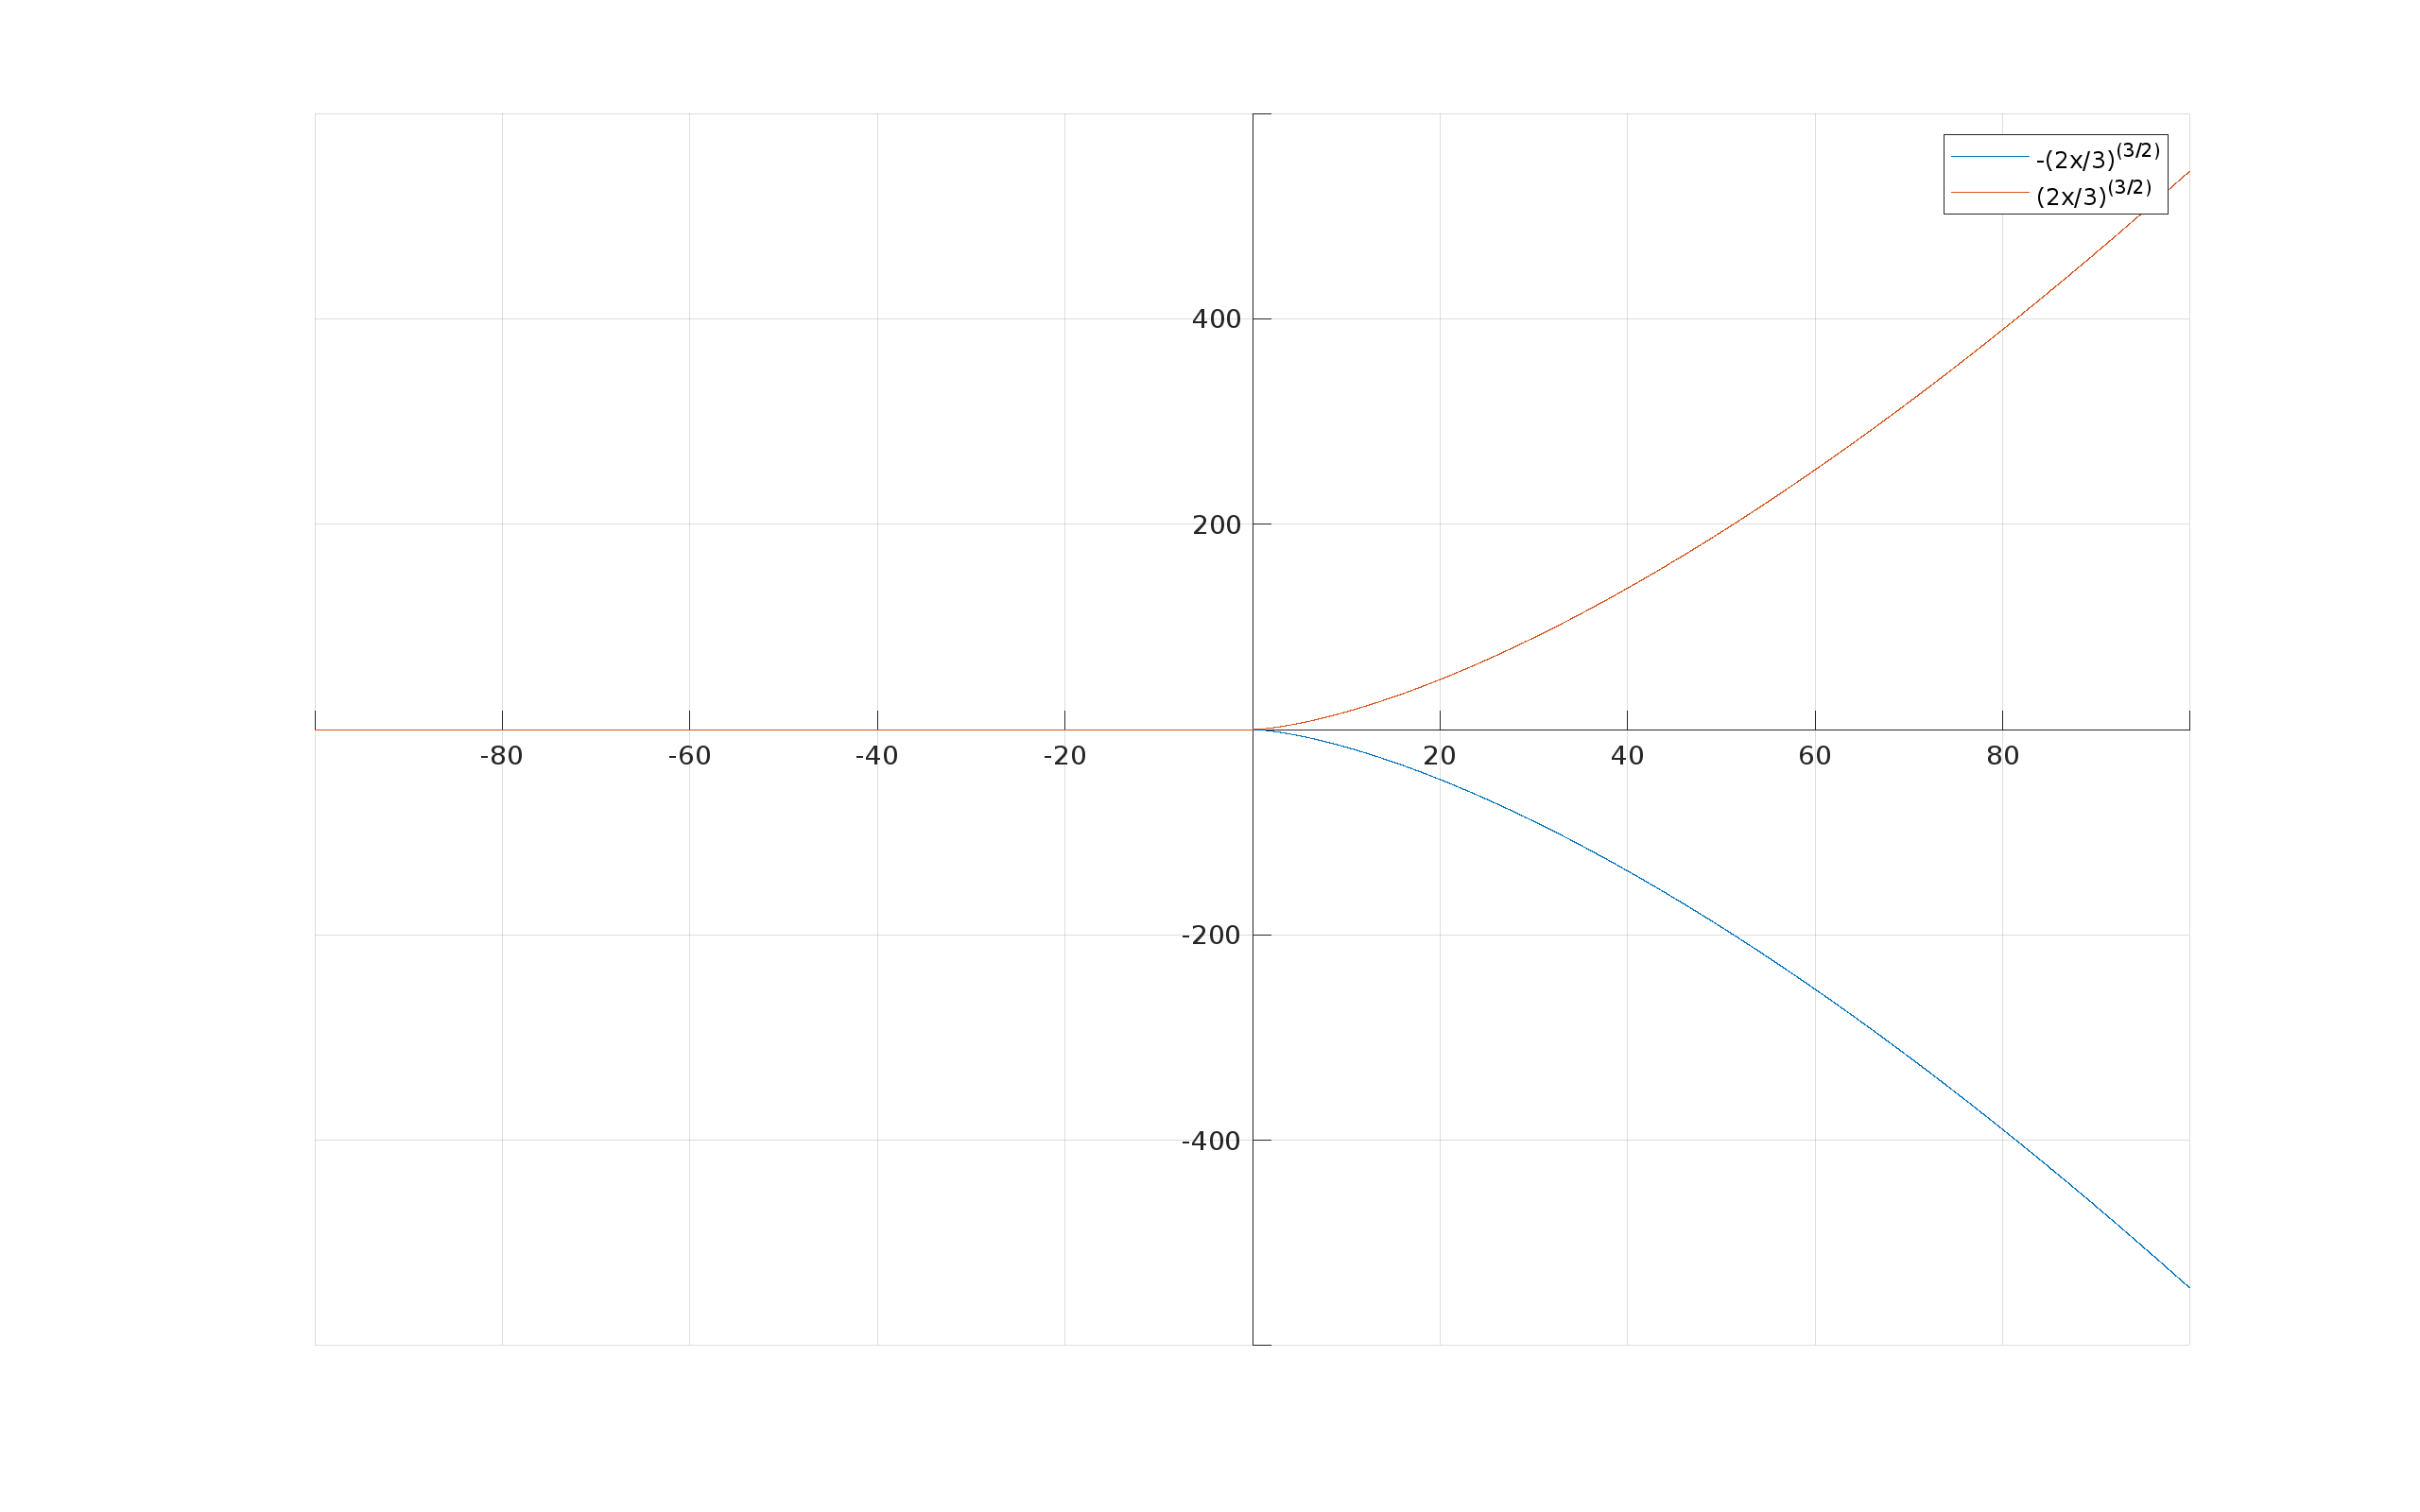
\includegraphics[width=1.0\textwidth]{Analisi2/figures/Phi.png}
    \caption{Grafico di $\varphi_2(x)=\left(\frac{2x}{3}\right)^{\frac{3}{2}}$ e $-\varphi_2(x)$.}
    \label{fig:phi}
\end{figure}

\subsubsection{EDO a variabili separabili}
\begin{definition}[EDO al primo ordine in forma normale a variabili separabili]
    \footnote{Slide 6 PDF 3.} Una EDO del primo ordine in forma normale (\ref{eq:EDO_lineare_ordine_1_forma_normale}) è detta a variabili separabili se è della forma
    \begin{equation}\label{eq:EDO_primo_ordine_forma_normale_variabili_separabili}
        y'(x) = f(x) g(y(x)),
    \end{equation}
    dove $f:I\subseteq \mathbb R\rightarrow\mathbb R,\, g: J\subseteq\mathbb R\rightarrow\mathbb R$.
\end{definition}

\paragraph{Nota:} Quando è stato trattato il problema lineare, l'equazione omogenea associata è un'equazione a variabili separabili. Si chiamano EDO a variabili separabili perché le variabili sono divise.

\paragraph{Cosa significa risolvere una EDO?} Significa trovare tutte le $y=y(x)$ definite su un opportuno intervallo per cui $y$ è derivabile e la derivata prima $y'$ verifica l'equazione (in questo caso \ref{eq:EDO_primo_ordine_forma_normale_variabili_separabili}). 

\begin{remark}
    Una EDO lineare del primo ordine omogenea in forma normale (\ref{eq:EDO_lineare_omogenea_associata_ordine_1_forma_normale}), ovvero del tipo
    \begin{equation*}
        y'(x) + a(x) y(x) = 0,
    \end{equation*}
    è a variabili separabili.
\end{remark}

\paragraph{Come si "separano" le variabili dalla equazione della forma (\ref{eq:EDO_primo_ordine_forma_normale_variabili_separabili})?} Per "separazione" delle variabili si intende la $x$ dalla $y(x)$ ed è svolta con i seguenti passaggi:
\begin{enumerate}
    \item determinare eventuali $\bar y\in\mathbb R$ [\footnotemark] per cui $g(\bar y)=0$, da cui è ottenuto
    \begin{equation}\label{eq:soluzione_EDO_variabili_separabili}
        y(x)\equiv \bar y,
    \end{equation}
    soluzione del problema. \footnote{$y(x)\equiv\bar y$ soluzione perché $g(y)=0$ e $y'=0$, dato che $\bar y$ è una funzione costante.} Inoltre, (\ref{eq:soluzione_EDO_variabili_separabili}) sono dette soluzioni singolari$_{\footnotemark}$ (o anche particolari$_{\footnotemark}$) della EDO.
    \item Considerando $y\neq\bar y$, è possibile separare le variabili dividendo per $g(y)$ (dove $g(y)\neq 0$ dato che $y\neq \bar y$, radice di $g$) la EDO, ovvero
    \begin{equation*}
        \frac{y'(x)}{g(y(x))} = \frac{f(x) \cancel{g(y(x))}}{\cancel{g(y(x))}} = f(x),
    \end{equation*}
    Da questa sono ottenute le soluzioni integrando rispetto ad $x$ ambo i membri, ovvero
    \begin{equation*}
        \int\frac{y'(x)}{g(y(x))}dx=\int f(x)dx,
    \end{equation*}
    dalle quali, ponendo $y=y(x)$ (cambiamento di variabile) e $dy = y'(x)dx$, è ottenuto
    \begin{equation*}
        \int \frac{1}{g(y)}dy = \int f(x)dx.
    \end{equation*}
    Siano $G$ e $F$ primitive di $\frac{1}{g}$ e $f$, è ottenuto
    \begin{equation*}
        G(y(x)) = F(x) + c.
    \end{equation*}
    [L'obiettivo è esplicitare $x$, quindi:] Se $G$ è invertibile si ha (la soluzione in forma implicita)
    \begin{equation*}
        y(x) = G^{-1} [F(x) + c].
    \end{equation*}
\end{enumerate}

\addtocounter{footnote}{-2}
\footnotetext{Tutte le soluzioni tali che $g(y)=0$ sono dette soluzioni singolari.}

\stepcounter{footnote}
\footnotetext{Particolari perché quando sono separate le variabili potrebbe accadere che una soluzione faccia parte dell'integrale generale per una scelta particolare della costante e quindi appartenga alla famiglia delle soluzioni.}

\stepcounter{footnote}
\footnotetext{Sono ricercati gli zeri di $g$, quindi la soluzionie di $g(y)=0$. Pertanto, data $\bar y$ soluzione (radice) del problema, con $y(x)\equiv \bar y$ soluzioni del problema, allora $g(y)=0$ (quindi $0=0$.}

\begin{example}[Esempio di applicazione del metodo precedente]\footnote{Slide 8-9 PDF 3.}
    \paragraph{Testo:} Determinare tutte le soluzioni della EDO del primo ordine (non lineare a variabili separabili)
    \begin{equation}\label{eq:esercizio_1_edo_variabili_separabili}
        y' = \underbrace{(1-y)(2-y)}_{g(y)}\underbrace{x}_{f(x)}.
    \end{equation}
    \paragraph{Svolgimento:}
    \begin{enumerate}
        \item Cerchiamo le soluzioni di $g(y)=0$, ovvero di $(1-y)(2-y) = 0$.\\
        Le soluzioni sono $y=1$ e $y=2$ (ovvero $y(x)=1$ o $y(x)=2$) e rappresentano le soluzioni costanti singolari della EDO a variabili separabili.
        \item Ora sono cercate le altre soluzioni (dividendo per $g(y)$).\\
        Data
        \begin{equation*}
            \frac{y'}{(1-y)(2-y)}=x,
        \end{equation*}
        integranado rispetto ad $x$ con cambio di variabile $y=y(x)$, è ottenuto
        \begin{equation*}
            \int \frac{y'(x)}{(1-y(x))(2-y(x))} dx = \int x\, dx.
        \end{equation*}
        Integrando con fratti semplici è ottenuto
        \begin{equation*}
            \int\frac{y'}{(1-y)(2-y)}dx = \int \frac{A}{1-y}+\frac{B}{2-y}dx,
        \end{equation*}
        dove
        \begin{equation*}
            1 = A(2-y)+B(1-y)=y(-A+B)+2A+B.
        \end{equation*}
        Tramite il principio di identità dei polinomi (Vedere Teorema \ref{th:principio_identità_polinomi})
        \begin{equation*}
            \begin{cases}
                -A-B&=0\\
                2A+B&=0
            \end{cases}\quad\Longrightarrow\quad
            \begin{cases}
                A=1\\
                B=1
            \end{cases}
        \end{equation*}
        quindi
    \begin{equation*}
        \int\frac{y'}{(1-y)(2-y)}dx \overset{y(x)=y,\, y'(x)dx=dy}{=} \int\frac{1}{1-y}dy-\int \frac{1}{2-y}dy = -\log(|1-y|) + \log(|2-y|) = \log\left|\frac{2-y}{1-y}\right|,
    \end{equation*}
    dove $y\neq 1$ (perché siamo al secondo passo).\\
    Dunque,
    \begin{equation*}
        \log\left|\frac{2-y}{1-y}\right| = \frac{x^2}{2}+c,
    \end{equation*}
    quindi
    \begin{equation*}
        \left|\frac{2-y}{1-y}\right| = \underbrace{e^{\frac{x^2}{2}+ c}}_{c_1e^{\frac{x^2}{2}}}>0.
    \end{equation*}
    Pertanto, è ottenuto che 
    \begin{equation}\label{eq:soluzioni_generali_esercizio_edo}
        \frac{2-y}{1-y}=\pm c_1 e^{\frac{x^2}{2}}=c e^{\frac{x^2}{2}},\quad c\in\mathbb R.
    \end{equation}
    \textbf{(\ref{eq:soluzioni_generali_esercizio_edo}) è la soluzione generale (anche detta "Famiglia generale"), ovvero l'integrale generale.}
    \paragraph{Intermezzo:} È necessario esprimere la soluzione generale (\ref{eq:soluzioni_generali_esercizio_edo}) in forma esplicita.\\
    Le soluzioni singolari sono $y=1$ e $y=2$. Dalla relazione (\ref{eq:soluzioni_generali_esercizio_edo}) è possibile ottenere $y=2$, ponendo $c=0$. Pertanto, la soluzione costante $y=2$ appartiene alla famiglia delle soluzioni (\ref{eq:soluzioni_generali_esercizio_edo}), con $c=0$.\\
    (\ref{eq:soluzioni_generali_esercizio_edo}) è una uguaglianza che non da la $y$ in funzione di $x$ (ciò che è ricercato), ovvero $G(x) = F(x)+c$.\\
    Alle volte le soluzioni singolari sono incluse nella famiglia generale delle soluzioni ottenuta separando le variabili, quindi al posto di unire le soluzioni ottenute dalla famiglia delle soluzioni separando le variabili e quelle singolari, è possibile ottenere le soluzioni singolari dalla (\ref{eq:soluzioni_generali_esercizio_edo}).\\
    (\ref{eq:soluzioni_generali_esercizio_edo}) è in forma implicita, quindi è necessario esplicitare la $y$ in funzione della $x$, ovvero quanto segue. $\qed$
    \begin{equation*}
        \begin{matrix}
            2-y &=& (1-y)\cdot c\cdot e^{\frac{x^2}{2}}\\
            2-y &=& ce^{\frac{x^2}{2}} - y\cdot c\cdot e^{\frac{x^2}{2}}\\
            (ce^{\frac{x^2}{2}} -1)y &=& c\cdot e^{\frac{x^2}{2}}-2 &\rightarrow& \text{non lineare.}
        \end{matrix}
    \end{equation*}
    Quindi, l'insieme delle soluzioni è dato da
    \begin{equation}\label{eq:integrale_generale_esercizio_edo_primo_ordine}
        \underbrace{y(x) = y(x,c)=\frac{c\cdot e^{\frac{x^2}{2}}-2}{c\cdot e^{\frac{x^2}{2}}-1}}_{\text{integrale generale (dipendente da $x$ e $c$)}},\quad c\in\mathbb R,
    \end{equation}
    dove $c\cdot e^{\frac{x^2}{2}}-1\neq 0$ (ovvero per tutte le $x$ dove (\ref{eq:integrale_generale_esercizio_edo_primo_ordine}) è definito).\\
    È ottenuto che:
    \begin{itemize}
        \item $y=2$ è ottenuto da (\ref{eq:integrale_generale_esercizio_edo_primo_ordine}), con $c=0$;
        \item $y=1$ non appartiene alla famiglia delle soluzioni.
    \end{itemize}
    Pertanto, \textbf{le soluzioni di (\ref{eq:esercizio_1_edo_variabili_separabili}) sono (\ref{eq:integrale_generale_esercizio_edo_primo_ordine}) e} $\boldsymbol{y=1}$. \footnote{$y=2$ appartiene già alla famiglia di soluzioni (\ref{eq:integrale_generale_esercizio_edo_primo_ordine}, quindi è esplicitato in quanto già incluso.}
    \end{enumerate}
\end{example}

\paragraph{Nota sul prossimo Esempio:} È aggiunta a (\ref{eq:integrale_generale_esercizio_edo_primo_ordine}) la condizione iniziale, ovvero: assunta una condizione iniziale, è posto il problema di Cauchy e definito qual è il più ampio intervallo sul quale è definita la soluzione. Determinare il più ampio è utile in quanto l'equazione (\ref{eq:integrale_generale_esercizio_edo_primo_ordine}) è non lineare. Pertanto, l'intervallo in questione conterrà il punto iniziale del problema ed è ricercato in modo tale che l'espressione (\ref{eq:integrale_generale_esercizio_edo_primo_ordine}) abbia senso e sia la soluzione della EDO (\ref{eq:esercizio_1_edo_variabili_separabili}).

\begin{example}[Problema di Cauchy per una EDO a variabili separabili]\footnote{Slide 11 PDF 4.}
    \paragraph{Testo:} Data la EDO del primo ordine non lineare a variabili separabili (\ref{eq:esercizio_1_edo_variabili_separabili})
    \begin{equation*}
        y' = \underbrace{(1-y)(2-y)}_{g(y)}\underbrace{x}_{f(x)},
    \end{equation*}
    con soluzioni costanti $y=1$ e $y=2$ e la soluzione generale (insieme delle soluzioni)
    \begin{equation}\label{eq:esercizio_1_intergrale_generale_problema_cauchy}
        y(x) = y(x,c)=\frac{c\cdot e^{\frac{x^2}{2}}-2}{c\cdot e^{\frac{x^2}{2}}-1},\quad c\in\mathbb R,
    \end{equation}
    con $c\cdot e^{\frac{x^2}{2}}-1\neq 0$.\\
    Risolvere il seguente problema di Cauchy (trovandone la soluzione) e specificare qual è il più ampio intervallo (rispetto all'inclusione $\subseteq$, \footnotemark) su cui è definita la soluzione,
    \begin{equation*}
        \begin{cases}
            y'&=(1-y)(2-y)x\quad\text{EDO non lineare}\\
            y(0) &= 3
        \end{cases}
    \end{equation*}
    \footnotetext{L'intervallo deve contenere il punto della condizione iniziale. Una volta definita la soluzione è necessario specificare dove è definita (su quale intervallo). Il più ampio intervallo è l'intervallo massimale rispetto all'inclusione nel quale la soluzione ha senso. È possibile osservare come le soluzioni costanti $y(x)=1$ e $y(x)=2$ non verifichino la condizione iniziale, quindi sono scartate. Ciò significa che la soluzione deve essere trovata utilizzando la formula (\ref{eq:esercizio_1_intergrale_generale_problema_cauchy}).}
    
    \paragraph{Svolgimento:} Le soluzioni $y(x)=1$ e $y(x)=2$ non verifichino la condizione iniziale, dunque è ricercata la soluzione utilizzando la formula (\ref{eq:esercizio_1_intergrale_generale_problema_cauchy}) imponendo la condizione iniziale ($y(0)=3$), ovvero
    \begin{equation*}
        3=\frac{c-2}{c-1},\quad \left(\rightarrow y(0)=\frac{ce^0-2}{ce^0-1}\right)
    \end{equation*}
    allora
    \begin{equation*}
        \begin{matrix}
            3c - 3 &=& c-2,\\
            2c &=& 1,\\
            c &=&\frac{1}{2}.
        \end{matrix}
    \end{equation*}
    La soluzione è dunque
    \begin{equation}\label{eq:soluzione_finale_esercizio_1_problema_cauchy}
        y(x)=\frac{\frac{1}{2}\cdot e^{\frac{x^2}{2}}-2}{\frac{1}{2}\cdot e^{\frac{x^2}{2}}-1} = \frac{e^{\frac{x^2}{2}}-4}{e^{\frac{x^2}{2}}-2}.
    \end{equation}
    \footnotemark L'intervallo più ampio contenente $x_0=0$, in cui la soluzione (\ref{eq:soluzione_finale_esercizio_1_problema_cauchy}) è ben definita (e contenuta) è determinata da
    \begin{equation*}
        \begin{matrix}
            e^{\frac{x^2}{2}}-2 \neq 0 &\rightarrow& e^{\frac{x^2}{2}}\neq 2 &\rightarrow& \frac{x^2}{2}\neq\ln 2 &\rightarrow& x^2\neq 2\ln2 &\rightarrow& x\neq\pm \sqrt{2\ln2}
        \end{matrix}
    \end{equation*}
    quindi l'intervallo più ampio in cui è definita la soluzione (\ref{eq:soluzione_finale_esercizio_1_problema_cauchy}) è
    \begin{equation*}
        I=(-\sqrt{2\ln2}, \sqrt{2\ln2})\ni 0.
    \end{equation*}
    \footnotetext{Affinché (\ref{eq:soluzione_finale_esercizio_1_problema_cauchy}) sia ben definito allora il denominatore di tale espressione deve essere diverso da 0.}
    
    \paragraph{Note su (\ref{eq:soluzione_finale_esercizio_1_problema_cauchy}):} è definita $\forall x\in\mathbb{R}\backslash\{\pm\sqrt{2\ln 2}\} $, ma per il problema di Cauchy richiesto di svolgere $\forall x\in I=(-\sqrt{2\ln2}, \sqrt{2\ln2})$.
    
    \paragraph{Nota su $\boldsymbol I$:} $I$ è una soluzione locale, ovvero le $x$ sono considerate vicine al punto iniziale. Quindi $y(x,c)$ è una soluzione in piccolo. Invece, se considerate le equazioni lineari ((\ref{eq:soluzione_finale_esercizio_1_problema_cauchy}) non è lineare), se i coefficienti della EDO sono continui (come nei nostri casi) la soluzione è definita in grande, ovvero su tutto l'intervallo nel quale i coefficienti della EDO sono continui.
    
    \paragraph{Nota:}
    È sbagliato affermare che la soluzione è definita $\forall x\in\mathbb R$ con $x\neq \pm\sqrt{2\log2}$ perché non è un intervallo, è ricercata la soluzione su un intervallo (ovvero un insieme limitato o illimitato contenente i punti in cui è contenuta la condizione iniziale). Affermando che $x\neq\pm\sqrt{2\log2}$ sono trovati 3 insiemi disgiunti
    \begin{equation}\label{eq:insiemi_esercizio_1_cauchy}
        (-\infty, -\sqrt{2\log2}), (-\sqrt{2\log2}, \sqrt{2\log2}), (\sqrt{2\log2}, +\infty)
    \end{equation}
    e questo non è un intervallo. Ciò ha un significato dal punto di vista fisico e matematico: dal punto di vista fisico la variabile indipendente può essere considerata come tempo, quindi è presente un sistema che evolve seguendo l'equazione differenziale definita che verifica la condizione iniziale. Quando è necessario stabilire il comportamento del sistema è controllato il comportamento in avanti (o all'indietro) partendo dal punto iniziale, dove se trovato un tempo per il quale il sistema perde di significato allora l'espressione non ha senso.\\
    Quindi, considerata la soluzione sull'intervallo è determinato l'intervallo massimale contenente la condizione iniziale.\\
    \paragraph{Significato fisico del problema di Cauchy:} La variabile indipendente può essere considerata come tempo, quindi è presente un sistema che evolve seguendo l'equazione differenziale definita che verifica la condizione iniziale. Se è trovato un tempo in cui il sistema perde significato (non esiste), non senso considerate il prima o il dopo (ad esempio $(-\infty, -\sqrt{2\log2})$ e $ (\sqrt{2\log2}, +\infty)$ in (\ref{eq:insiemi_esercizio_1_cauchy})) e quindi è considerato l'insieme massimale contente l'istante iniziale in cui il sistema fisico ha significato.
    \paragraph{Significato dal punto di vista matematico:} Dal punto di vista matematico non è possibile considerare $y(x)$ soluzione al problema di Cauchy su intervalli disgiunti come in (\ref{eq:insiemi_esercizio_1_cauchy})), perché il punto iniziale non è in $(-\infty, -\sqrt{2\log2})$ o $ (\sqrt{2\log2}, +\infty)$. Quindi la condizione iniziale determina la soluzione e l'unicità$_{\footnotemark}$ di questa nell'insieme che la contiene.
\end{example}
\footnotetext{Se considerati insiemi disgiunti, fissando la condizione iniziale, l'unicità sarebbe persa perché il punto iniziale non è in $(-\infty, -\sqrt{2\log2})$ o $ (\sqrt{2\log2}, +\infty)$.}

\begin{example}\footnote{Slide 14 PDF 4.}
    \paragraph{Testo:} Risolvere il problema di Cauchy
    \begin{equation*}
        \begin{cases}
            y' &=xy+2x\quad\text{(EDO lineare)}\\
            y(0)& = 2
        \end{cases}
    \end{equation*}
    \paragraph{Svolgimento:} Trasformazione in forma normale (ovvero $y'-a(x)y=f(x)$):
    \begin{equation*}
        y'-xy = 2x.
    \end{equation*}
    Dato che $a(x)=-x$, allora $A(x)=-\int xdx=-\frac{x^2}{2}$. Utilizzando la formula risolutiva (\ref{eq:soluzione_problema_cauchy_primo_ordine_coeff_costanti}) è ottenuto
    \begin{equation*}
        y(x) = c\cdot e^{-A(x)} + e^{-A(x)}\int f(x) e^{A(x)} dx,
    \end{equation*}
    quindi la soluzione è
    \begin{equation*}
        y(x)=y(x,c)= c\cdot e^{\frac{x^2}{2}}+ e^{\frac{x^2}{2}}\int 2xe^{-\frac{x^2}{2}}dx = c\cdot e^{\frac{x^2}{2}}+ e^{\frac{x^2}{2}}\left(-2 e^{-\frac{x^2}{2}}\right)=c\cdot e^{\frac{x^2}{2}}-2,\quad c\in\mathbb R.
    \end{equation*}
    Imponendo $y(0)=1$, allora
    \begin{equation*}
        1=c\cdot e^{0} -2\quad \rightarrow\quad c = 3,
    \end{equation*}
    quindi la soluzione è
    \begin{equation*}
        y(x) = 3e^{\frac{x^2}{2}}-2,\quad x\in\mathbb R.
    \end{equation*}
    \paragraph{Nota sulla soluzione:} In questo caso $y(x)$ è una soluzione in grande perché definita su tutta $\mathbb R$.
\end{example}

\begin{example}[Problema di Cauchy a variabili separabili]\footnote{Slide 16 PDF 4.}
    \paragraph{Testo:} Risolvere il seguente problema di Cauchy a variabili separabili
    \begin{equation*}
        \begin{cases}
            u' &= \underbrace{(1+u^2)}_{g(t)}\underbrace{\sin(t)}_{f(t)} \text{ con } u=u(t) \text{ soluzione}\\
            u(0) &= 1
        \end{cases}
    \end{equation*}
    È possibile separare le variabili a condizione che $1+u^2\neq 0$ (ovvero $u^2\geq1$). Dividendo per $g(x)$ è ottenuto
    \begin{equation*}
        \frac{u'(t)}{1+u^2(t)} = \sin t,
    \end{equation*}
    ed integrando
    \begin{equation*}
        \int \frac{u'(t)}{1+u^2(t)}dt = \int\sin t \,dt,
    \end{equation*}
    per sostituzione, con $u=u(t)$ e $dv=u'(t)\,dt$ è ottenuto che
    \begin{equation*}
        \int \frac{u'}{1+u^2}du = -\cos t + c,
    \end{equation*}
    quindi
    \begin{equation}\label{eq:arctan_esercizio_cauchy}
        \arctan u(t) = -\cos(t) + c.
    \end{equation}
    \paragraph{Intermezzo:} È possibile scrivere chi è $u(t)$. (\ref{eq:arctan_esercizio_cauchy}) è la versione implicita della soluzione, è possibile invertire la $G$, la quale è una primitiva di $\int \frac{u'}{1+u^2}du$ e quindi è utilizzata la funzione inversa (ovvero la tangente). Quindi è ottenuto quanto segue. $\qed$
    \begin{equation*}
        u(t) = \tan(-\cos t + c)= \underbrace{u(t, c)}_\text{int. gen.}\in\mathbb R.
    \end{equation*}
    Imponendo la condizione iniziale è ottenuto che
    \begin{equation*}
       \begin{matrix}
            \arctan u(0) &=& -\cos 0 + c\\
            &\Vertrarrow&\\
            \arctan 1 &=& -1 + c\\
            &\Vertrarrow&\\
            \frac{\pi}{4} &=& -1 + c\\
            &\Vertrarrow&\\
            c &=& 1+\frac{\pi}{4}
       \end{matrix}
    \end{equation*}
    Dunque la soluzione è data da
    \begin{equation*}
    	u(t)=\tan\left(-\cos t + 1 + \frac{\pi}{4}\right)\quad \forall\left(-\cos t + 1 + \frac{\pi}{4}\right)\in\left(-\frac{\pi}{2}, \frac{\pi}{2}\right).
    \end{equation*}
\end{example}

\begin{example}\footnote{Slide 16 PDF 4.}
    \paragraph{Testo:} Risolvere il problema di Cauchy
    \begin{equation*}
        \begin{cases}
            y' + 2t y^2 &= 0\\
            y(0) &= -1
        \end{cases}
    \end{equation*}
    \paragraph{Nota:} $y' + 2t y^2 = 0$ è una EDO del primo ordine non lineare a variabili separabili. Inoltre, le soluzioni sono del tipo $y=y(t)$. $\qed$\\
    Quindi,
    \begin{equation*}
        y' = -2 t y^2,
    \end{equation*}
    dove
    \begin{itemize}
        \item $f(t) = -2t$,
        \item $g(t) = y^2$,
    \end{itemize}
    entrambe funzioni definite su tutto $\mathbb R$. È possibile osservare che $y(t)=0$ è soluzione di
    \begin{equation*}
        y' + 2ty^2 = 0,
    \end{equation*}
    ma questa non verifica la condizione iniziale, quindi sono separate le variabili (dividendo per $y^2$).
    \paragraph{Nota:} È possibile dividere subito per $y^2$ in quanto la condizione $y=0$ non verifica la condizione iniziale, quindi non si puo' verificare una divisione per 0.$\qed$\\
    Data
    \begin{equation*}
    	\frac{y'(t)}{y^(t)}=2t,
    \end{equation*}
    integrando
    \begin{equation*}
    	\int\frac{y'(t)}{y^2(t)}dt=-2\int t\, dt
    \end{equation*}
    è ottenuto
    \begin{equation*}
    	-\frac{1}{y(t)} = -t^2+c,
    \end{equation*}
    ovvero
    \begin{equation*}
	\frac{1}{y(t)} = t^2-c,\quad c\in\mathbb{R}.
    \end{equation*}
    Quindi,
    \begin{equation*}
        1 = y t^2 - yc = y(t^2-c),
    \end{equation*}
    allora
    \begin{equation*}
        y(t) = \frac{1}{t^2-c}\quad\text{oppure}\quad y(t) = \frac{1}{t^2+c}.
    \end{equation*}
    (le quali sono funzioni diverse, ma l'utilizzo finale non cambia e quindi è utilizzata la forma più comoda.)
    \footnote{Per definire la soluzione è necessario che il denominatore sia diverso da 0 e ciò è legato al valore della costante. Con valori della costante positivi non ci sono problemi di definizione del dominatore, con valori negativi sono necessari esclusioni. Inoltre, è necessario trovare l'intervallo dove la soluzione e ben definita (ovvero l'intervallo contente $t=0$), quindi $t^2+c\neq 0$.}
    Imponiamo la condizione iniziale $y(0) = -1$,
    \begin{equation*}
        1=\frac{1}{0+c},
    \end{equation*}
    quindi $c=-1$. La soluzione del problema è
    \begin{equation*}
        y(t) = \frac{1}{t^2 -1},\quad \forall t\in(-1,1)\ni 0,
    \end{equation*}
    se $t^2 -1\neq 0$, ovvero $t\neq \pm 1$.
    \paragraph{Nota sulla soluzione:} La soluzione è considerata nell'intervallo massimale $(-1, 1)$ (il quale contiene $t=0$). Inoltre, l'espressione $\frac{1}{t^2 -1}$ ha senso in tutti gli intervalli in cui $t^2-1\neq 0$, ma è necessario considerare l'intervallo contenente il punto iniziale.
\end{example}

\begin{example}\footnote{Slide 19 PDF 4.}
    \paragraph{Testo:} Risolvere il problema di Cauchy
    \begin{equation*}
        \begin{cases}
            y'(x)+\frac{3x^2}{5+x^3}y(x) &= \sqrt[3]{x}\\
            y(0) &= 1
        \end{cases}
    \end{equation*}
    e precisare qual è il più ampio intervallo su cui la soluzione trovata è definita.
    \paragraph{Nota:} La EDO è lineare del primo ordine e della forma $y'+a(x)y=f(x)$, dove $a(x)=\frac{3x^2}{5+x^3}$ e $f(x) = \sqrt[3]{x}$.
    \paragraph{Svolgimento:} La EDO è definita $\forall x\in\mathbb R : x\neq-\sqrt[3]{5}$ (perché $5+x^3\neq 0$).\\
    La condizione iniziale è assegnata in $x_0=0$ e poiché $x_0>-\sqrt[3]{x}$, è considerata la soluzione sull'intervallo $I=(-\sqrt[3]{5}, +\infty)\ni 0$. \footnote{La soluzione al problema è in grande sull'intervallo.}\\
    \begin{equation*}
        A(x) = \int \frac{3x^2}{5+x^3} dx = \log(5+x^3),\quad \forall x\in I=(-\sqrt[3]{5}, +\infty),
    \end{equation*}
    quindi, l'integrale generale è
    \begin{equation*}
        \begin{matrix}
            \boldsymbol{y(x)} &=& c\cdot e^{-\log(5+x^3)} + e^{-\log(5+x^3)}\int e^{\log(5+x^3)} \sqrt[3]{x}\, dx &=& y(x,c)\\
            &=& \underbrace{\frac{1}{5+x^3}}_{\footnotemark}\left[c+\int (5+x^3)\sqrt[3]{x}dx\right] \overset{\footnotemark}{=} \frac{1}{5+x^3}\left(c+\int 5\sqrt[3]{x}dx+\int x^{\frac{10}{3}} dx\right) &=& \boldsymbol{\frac{1}{5+x^3}\left(c+5\cdot\frac{3}{4}x^{\frac{4}{3}} + \frac{3}{13}x^{\frac{13}{3}}\right)},
        \end{matrix}
    \end{equation*}
    \addtocounter{footnote}{-1}
    \footnotetext{Inversa di $e^{-\log(5+x^3)}$.}

    \stepcounter{footnote}
    \footnotetext{Linearità dell'integrale.}
    
    \noindent ovvero,
    \begin{equation*}
        y(x)= \frac{1}{5+x^3}\left(c+\cdot\frac{15}{4}x^{\frac{4}{3}} + \frac{3}{13}x^{\frac{13}{3}}\right).
    \end{equation*}
    Imponendo la condizione iniziale $y(0) = 1$ è ottenuto
    \begin{equation*}
        1=\frac{1}{5}\cdot c \quad\rightarrow\quad c=5,
    \end{equation*}
    quindi la soluzione al problema di Cauchy è
    \begin{equation*}
        y(x) = \frac{1}{5+x^3} \left(\frac{15}{4}x^{\frac{4}{3}} + \frac{3}{13}x^{\frac{13}{3}}+5\right),\quad \forall x\in(-\sqrt[3]{x}, +\infty)
    \end{equation*}
\end{example}

\begin{exercise}[Da fare a casa]
    Risolvere il problema di Cauchy
    \begin{equation*}
        \begin{cases}
            y'(x) = -\frac{\sin(2x)}{1+\cos^2(x)}y(x) + \sin x\\
            y(\pi)= 1
        \end{cases}
    \end{equation*}
    Precisare qual è il più ampio intervallo (massimale contente $\pi$) in cui la soluzione è definita.
\end{exercise}

\subsection{Risultati importanti sulle EDO del secondo ordine a coefficienti costanti}\footnote{Slide 22 PDF 4.} 
Per trovare la soluzione di questo tipo di EDO, l'integrale generale, esiste un metodo infallibile, ovvero: trovare la soluzione di un'equazione algebrica di grado 2 di campo complesso.\\
In matematica un'equazione del tipo $x^2+1=0$ non ha soluzioni in campo reale ma nel campo complesso coniugato. Quindi, affinché tale equazione abbia sempre soluzione è considerato il campo complesso. Per questo è utilizzato il Teorema \ref{th:fondamentale_algebra} fondamentale dell'Algebra (fatto a MDL o Algebra Lineare), il quale afferma che l'equazione considerata ha sempre almeno una soluzione nel campo complesso ed in particolare le soluzioni possono essere reali, distinte o coincidenti, ma se sono complesse sono complesse coniugate (intese come numeri complessi coniugati, vedere Definizione \ref{def:complesso_coniugato}).

\begin{definition}[EDO lineare del secondo ordine]\label{def:edo_lineare_secondo_ordine}
    Una EDO del secondo ordine si dice lineare se della forma
    \begin{equation}\label{eq:edo_lineare_secondo_ordine}
        a_2(x)y''(x)+a_1(x)y'(x)+a_0(x)y(x) = f(x),
    \end{equation}
    dove i coefficienti $a_i(x),\, i=0,1,2$ ed il termine noto $f(x)$ sono $C^0(I)$.
\end{definition}

\paragraph{IMPORTANTE:} Se $f(x)\neq 0$, allora (\ref{eq:edo_lineare_secondo_ordine}) è detta \textbf{completa}.

\paragraph{IMPORTANTE:} \textbf{Saranno considerate solo EDO del secondo ordine a coefficienti costanti.}

\begin{definition}[EDO lineare del secondo ordine in forma normale]
    La EDO lineare del secondo ordine (\ref{eq:edo_lineare_secondo_ordine}) è in forma normale se $a_2(x)=1$, ovvero
    \begin{equation}\label{eq:edo_lineare_secondo_ordine_forma_normale}
        y''(x)+a_1(x)y'(x)+a_0(x)y(x) = f(x).
    \end{equation}
\end{definition}

\begin{definition}[EDO lineare del secondo ordine omogenea associata]
    La EDO omogenea associata a (\ref{eq:edo_lineare_secondo_ordine}) è
    \begin{equation}\label{eq:edo_omogenea_associata_lineare_secondo_ordine}
        y''(x)+a_1(x)y'(x)+a_0(x)y(x) = 0.
    \end{equation}
\end{definition}

\paragraph{Nota:} Per la EDO completa della forma (\ref{eq:edo_lineare_secondo_ordine}) esiste l'integrale generale della forma integrale generale dell'omogenea + integrale particolare della non omogenea, ovvero il Teorema (\ref{th:rappresentazione_integrale_generale_EDO_lineare}) vale $\forall n\geq1$.

\paragraph{IMPORTANTE:} Il Teorema (\ref{th:rappresentazione_integrale_generale_EDO_lineare}) vale $\forall n\geq1$, quindi \textbf{il problema diventa trovare l'integrale generale della EDO omogenea in forma normale e l'integrale particolare della non omogenea}.

\paragraph{Rappresentazione alternativa dell'integrale generale per EDO di ordine 2:} L'integrale generale rappresentato in forma (\ref{eq:rappresentazione_integrale_generale_EDO_lineare}) può essere visto in modo informale per le EDO del secondo ordine come
\begin{equation*}
\int \text{ generale di (\ref{eq:edo_lineare_secondo_ordine_forma_normale})}=\int{\text{ generale di (\ref{eq:edo_omogenea_associata_lineare_secondo_ordine})}} + \int\text{ particolare di (\ref{eq:edo_lineare_secondo_ordine_forma_normale})}.
\end{equation*}

\begin{remark}[Non ufficiale]\label{rem:dimensione_spazio_vettoriale_edo_secondo_ordine}
    Lo spazio delle soluzioni di una EDO di ordine $n=2$ è uno spazio vettoriale di dimensione $n=2$, quindi per trovare una soluzione qualsiasi dell'omogenea servono $n=2$ soluzioni linearmente indipendenti (e da queste, com'è noto per AL, sono trovate tutte le altre).
\end{remark}

\noindent \textbf{L'Osservazione \ref{rem:dimensione_spazio_vettoriale_edo_secondo_ordine} si traduce in quanto segue:} se le funzioni $y_1(x),y_2(x)$ sono soluzioni di (\ref{eq:edo_omogenea_associata_lineare_secondo_ordine}), allora
\begin{enumerate}
    \item $y_1(x)$ e $y_2(x)$ sono linearmente indipendenti,
    \item ogni altra soluzione è una combinazione lineare di $y_1(x)$ e $y_2(x)$\footnote{Ciò segue dalla linearità della EDO, dovuto all'operatore $L$ associato ad ogni EDO lineare. $L$ è un funzionale che associa una funzione di classe $C^n(I)$ ad una funzione continua ($C^0(I)$), ovvero associa una funzione $\varphi$ a $a_n\varphi^n+\hdots+a_0\varphi^0$. Dalla linearità dell'operatore $L$ segue che se $\varphi_1$ e $\varphi_2$ sono soluzioni della EDO, anche la loro combinazione lineare è soluzione della EDO (come visto nel caso generale).}, allora \textbf{l'integrale generale generale della omogenea associata (\ref{eq:edo_omogenea_associata_lineare_secondo_ordine}) è}
    \begin{equation*}
        c_1 y_1(x) + c_2 y_2(x),
    \end{equation*}
    al variare di $c_1,c_2\in\mathbb R$.
\end{enumerate}

\paragraph{Soluzioni della omogenea associata (\ref{eq:edo_omogenea_associata_lineare_secondo_ordine}): }\footnote{Per ottenere tutte le soluzioni sono necessarie 2 soluzioni linearmente indipendenti, dato che lo spazio vettoriale di una EDO lineare omogenea ha dimensione 2. Dalle due soluzioni è costruita un sistema fondamentale di soluzioni.\\
Analogamente, per $\mathbb R^n$ la base canonica, la quale è una \gls{base ortonormale}, permette di scrivere vettori in $\mathbb R^n$ come combinazione lineare di $e_1,e_2,\hdots, e_n$. Quindi $e_1,e_2,\hdots, e_n$ formano un sistema fondamentale per lo spazio $\mathbb R^n$ perché gli elementi dello spazio sono espressi come combinazione lineare della base canonica.} Quindi, se $y_1(x)$ e $y_2(x)$ sono soluzioni linearmente indipendenti su $I$ della EDO omogenea associata (\ref{eq:edo_omogenea_associata_lineare_secondo_ordine}) (ovvero, sono la base utilizzata per scrivere una soluzione qualsiasi) allora ogni soluzione di (\ref{eq:edo_omogenea_associata_lineare_secondo_ordine}) (elemento dell'integrale generale di (\ref{eq:edo_omogenea_associata_lineare_secondo_ordine})) è una loro combinazione lineare (cioè $y_1(x)$ e $y_2(x)$ formano un sistema fondamentale di funzioni).

\footnote{Se presa una loro combinazione lineare di $y_1(x)$ e $y_2(x)$ e è posta uguale a 0, l'unica soluzione al problema è che $c_1$ e $c_2$ siano 0 $\forall x\in I$. Segue quanto scritto.} Se $y_1(x)$ e $y_2(x)$ sono soluzioni della EDO omogenea (\ref{eq:edo_omogenea_associata_lineare_secondo_ordine})) e sono linearmente indipendenti su $I$ ($\forall x\in I$), significa che
\begin{equation*}
    c_1 y_1(x) + c_2 y_2(x) = 0 \iff c_1=c_2=0.
\end{equation*}
Ciò significa che
\begin{equation}\label{eq:sistema_fondamentale_soluzioni_EDO_omogena_associata}
    \{y_1(x), y_2(x)\}
\end{equation}
formano un sistema fondamentale di soluzioni per (\ref{eq:edo_omogenea_associata_lineare_secondo_ordine}) e quindi ogni soluzione su $I$ di (\ref{eq:edo_omogenea_associata_lineare_secondo_ordine}) si scrive come loro combinazione lineare.

\paragraph{Nota su (\ref{eq:sistema_fondamentale_soluzioni_EDO_omogena_associata}):} Quanto scritto significa che l'integrale generale di una EDO del secondo ordine dipende dalle 2 costanti $c_1$ e $c_2$, oltre che dalla variabile $x$ (una EDO del primo ordine dipende da 1 costante).

\paragraph{Spiegazione di (\ref{eq:sistema_fondamentale_soluzioni_EDO_omogena_associata}):} Gli elementi di $\mathbb R^n$ sono rappresentabili tramite la base canonica (la quale è una \gls{base ortonormale}).\\
Un vettore può essere rappresentato come combinazione lineare con la base canonica, ad esempio: $(1,2)\in\mathbb R^2$ può essere espresso come $1\uline e_1 + 2\uline e_2=\uline u=(1,2)$. Lo stesso vale con (\ref{eq:sistema_fondamentale_soluzioni_EDO_omogena_associata}): $y_1(x)$ e $y_2(x)$ sono due soluzioni del problema omogeneo ed è possibile dimostrare, tramite la linearità del problema, che la loro combinazione lineare è anche la soluzione. Dato che l'obiettivo è trovare tutte le soluzioni (generare lo spazio delle soluzioni), è sufficiente avere due soluzioni indipendenti (due perché la EDO è di ordine due e lo spazio delle soluzioni è di dimensione due). La lineare indipendenza delle soluzioni sull'intervallo $I$ segue da AL:  la combinazione di $y_1(x)$ e $y_2(x)$ è linearmente indipendente (tale combinazione deve essere $=0$) se e solo se i coefficienti della combinazione sono tutti 0.\\
\textbf{Riassumendo:} Per trovare una soluzione qualsiasi del problema omogeneo (\ref{eq:edo_omogenea_associata_lineare_secondo_ordine}) è sufficiente trovare due soluzioni linearmente indipendenti del problema, le quali formano un sistema fondamentale di soluzioni.$\qed$

Data la Definizione \ref{def:edo_lineare_secondo_ordine} di EDO lineare del secondo ordine, allora è possibile la seguente.
\begin{definition}[EDO lineare del secondo ordine a coefficienti costanti]
	Una EDO lineare del secondo ordine è a coefficienti costanti se della forma
	\begin{equation}\label{eq:edo_lineare_secondo_ordine_coefficienti_costanti}
		a y'' + by' + cy =  f(x),\quad a,b,c\in\mathbb{R},\quad a\neq 0,
	\end{equation}
	dove $a=a_0(x), b=a_1(x), c=a_2(x)\in C^0(I)$ funzioni costanti e $f(x)\in C^0(I)$, con $I\subseteq\mathbb{R}$ intervallo.
\end{definition}

\begin{definition}[EDO lineare del secondo ordine omogenea a coefficienti costanti]
	Una EDO lineare del secondo ordine omogenea associata a (\ref{eq:edo_lineare_secondo_ordine_coefficienti_costanti}) è a coefficienti costanti se della forma
	\begin{equation}\label{eq:edo_lineare_secondo_ordine_omogenea_coefficienti_costanti}
		a y'' + by' + cy =  0,\quad a,b,c\in\mathbb{R},\quad a\neq 0,
	\end{equation}
	dove $a=a_0(x), b=a_1(x), c=a_2(x)\in C^0(I)$ funzioni costanti, con $I\subseteq\mathbb{R}$ intervallo.
\end{definition}

\paragraph{Considerazioni su (\ref{eq:edo_lineare_secondo_ordine_coefficienti_costanti}) e (\ref{eq:edo_lineare_secondo_ordine_omogenea_coefficienti_costanti}):}
\begin{enumerate}
	\item $a,b,c \in\mathbb{R}$ e $a\neq 0$,
	\item $x\in I$.
\end{enumerate}

\subsubsection{Ricerca dell'integrale generale \texorpdfstring{$\boldsymbol{\bar z(x)}$}{z(x)} di (\ref{eq:edo_lineare_secondo_ordine_omogenea_coefficienti_costanti})}
Per cercare la soluzione di (\ref{eq:edo_lineare_secondo_ordine_omogenea_coefficienti_costanti}) è necessario distinguere due casi:
\begin{enumerate}
	\item Se $b=c=0$ (sono identicamente nulle), l'equazione (\ref{eq:edo_lineare_secondo_ordine_omogenea_coefficienti_costanti}) diventa
	\begin{equation*}
		a y''=0,
	\end{equation*}
	quindi $y'(x)=c_1$ (è una costante). Integrando è ottenuto l'integrale generale dell'omogenea
	\begin{equation*}
		y(x)=y(x,c_1,c_2) 
		= c_1 x+c_2,\quad c_1,c_2\in\mathbb{R}.
	\end{equation*}
	\item Se $b$ e $c$ non sono identicamente nulle, per trovare l'integrale generale di (\ref{eq:edo_lineare_secondo_ordine_omogenea_coefficienti_costanti}) gli è associata una equazione algebrica di secondo grado in $\mathbb{C}$, detta equazione caratteristica di (\ref{eq:edo_lineare_secondo_ordine_omogenea_coefficienti_costanti}), della forma
	\begin{equation}\label{eq:equazione_caratteristica_associata_omogenea}
		\underbrace{a\lambda^2 + b\lambda + c}_{p(\lambda)} = 0,\quad\lambda\in\mathbb{R}.
	\end{equation}
	\footnote{L'equazione (\ref{eq:equazione_caratteristica_associata_omogenea}) è considerata in campo complesso perché $\Delta = b^2-4ac<0$, quindi le soluzioni a tale equazioni sono complesse. Per il Teorema \ref{th:fondamentale_algebra} fondamentale dell'algebra, l'equazione ha sempre due soluzioni nel campo complesso se $\Delta<0$ o reali se $\Delta>0$.} Quando $p(\lambda)=0$? Formalmente le soluzioni di (\ref{eq:equazione_caratteristica_associata_omogenea}) sono date da
	\begin{equation*}
		\lambda_{1,2} = \frac{-b\pm\sqrt{\Delta}}{2a}.
	\end{equation*}
\end{enumerate}

\begin{remark}[Non ufficiale]
	Tramite l'operatore $L$ associato alla EDO lineare omogenea di secondo grado (\ref{eq:edo_lineare_secondo_ordine_omogenea_coefficienti_costanti}), definito come 
	\begin{equation*}
		L(\varphi(x)):=a\varphi''(x) + b\varphi(x)'(x) + c\varphi(x),\quad \varphi\in C^2(I).
	\end{equation*}
	è possibile scrivere (\ref{eq:edo_lineare_secondo_ordine_omogenea_coefficienti_costanti}) come
	\begin{equation*}
		Ly(x)=0.
	\end{equation*}
	Quindi risolvere (\ref{eq:edo_lineare_secondo_ordine_omogenea_coefficienti_costanti}) significa trovare le $y$ per le quali
	\begin{equation}\label{eq:equivalenza_edo_lineare_secondo_grado_omogenea_operatore}
		(\ref{eq:edo_lineare_secondo_ordine_omogenea_coefficienti_costanti})\equiv L(y(x)) = 0.
	\end{equation}
	Inoltre, per risolvere il problema non omogoneo è posto $f(x)$ al posto di 0 in (\ref{eq:equivalenza_edo_lineare_secondo_grado_omogenea_operatore}).
\end{remark}

\begin{proposition}\footnote{Slide 3 PDF 5.}\label{prop:e^lambdax_soluzione_omogenea_secondo_grado_lineare}
	\begin{equation*}
		y(x)=e^{\lambda x}\text{ è soluzione (reale o complessa\footnotemark) di (\ref{eq:edo_lineare_secondo_ordine_omogenea_coefficienti_costanti})} \iff \lambda \text{ è radice (zero) dell'equazione } p(\lambda)=0,
	\end{equation*}
	dove $p(\lambda)=0$ è (\ref{eq:equazione_caratteristica_associata_omogenea}).
\end{proposition}
\footnotetext{Dipende da $\lambda$ se è complessa o reale.}
\begin{proof}
	È necessario dimostrare che $L(e^{\lambda x})=0\iff p(\lambda)=0$.
	\begin{equation*}
		L(e^{\lambda x}) = a(e^{\lambda x})''+ b(e^{\lambda x})'+ c e^{\lambda x} = a(\lambda^2 e^{\lambda x}) + b\lambda e^{\lambda x} + c e^{\lambda x} = e^{\lambda x} (a\lambda ^2 + b\lambda + c),
	\end{equation*}
	quindi
	\begin{equation*}
		L(e^{\lambda x}) = 0 \iff a\lambda^2 + b\lambda + c=p(\lambda) = 0.
	\end{equation*}
\end{proof}

\paragraph{Osservazione sulla dimostrazione:} Se $\lambda$ è una radice dell'equazione caratteristica associata a (\ref{eq:edo_lineare_secondo_ordine_omogenea_coefficienti_costanti}) (ovvero $\lambda$ tale che $a\lambda^2 + b\lambda + c= 0$), allora la funzione $y(\lambda)=e^{\lambda x}$ è una soluzione reale o complessa della EDO lineare omogenea di secondo ordine a coefficienti costanti (\ref{eq:edo_lineare_secondo_ordine_omogenea_coefficienti_costanti}).\\
Quindi è necessario studiare le radici (zeri) della equazione caratteristica (o equazione algebrica di secondo grado con soluzioni in $\mathbb{C}$) (\ref{eq:equazione_caratteristica_associata_omogenea}). A seconda che $\Delta$ sia $>, <$ o = 0, ci saranno due soluzioni reali distinte, due soluzioni reali coincidenti o due soluzioni complesse coniugate.

\paragraph{Determinazioni delle soluzioni linearmente indipendenti della EDO lineare omogenea di secondo ordine a coefficienti costanti (\ref{eq:edo_lineare_secondo_ordine_omogenea_coefficienti_costanti}):} Siano le due radici $\lambda_{1,2}=\frac{-b\pm\sqrt{\Delta}}{2a}$ (soluzioni del polinomio caratteristico), sono distinti i tre seguenti casi dove le soluzioni della EDO lineare omogenea di secondo ordine a coefficienti costanti (\ref{eq:edo_lineare_secondo_ordine_omogenea_coefficienti_costanti}):
\begin{enumerate}
	\item Caso $\Delta>0$:
	\begin{equation}\label{eq:soluzioni_omogenea_secondo_grado_delta_negativa}
		y_1(x) = e^{\lambda_1 x},\, y_2(x) = e^{\lambda_2 x},\quad \lambda_1,\lambda_2\in\mathbb{R}\text{ e } \lambda_1\neq\lambda_2,
	\end{equation}
	quindi l'integrale generale di (\ref{eq:edo_lineare_secondo_ordine_omogenea_coefficienti_costanti}) è
	\begin{equation*}
		\boldsymbol{\bar z(x)} = c_1 y_1(x)+ c_2y_2(x) = \boldsymbol{c_1 e^{\lambda_1 x} + c_2(x) e^{\lambda_2 x}}.
	\end{equation*}
	\item Caso $\Delta = 0$:
	\begin{equation}\label{eq:soluzioni_omogenea_secondo_grado_delta_zero}
		y_1(x) = e^{\lambda x},\, y_2(x)=x e^{\lambda x},\quad \lambda_1=\lambda_2=\lambda=\frac{-b}{2a}\in\mathbb{R},
	\end{equation}
	quindi l'integrale generale di (\ref{eq:edo_lineare_secondo_ordine_omogenea_coefficienti_costanti}) è
	\begin{equation*}
		\boldsymbol{\bar z(x) = e^{\lambda x}(c_1+c_2 x)}, 
	\end{equation*}
	\item Caso $\Delta<0$:
	\begin{equation}\label{eq:soluzioni_omogenea_secondo_grado_delta_positiva}
		y_1(x) = e^{\alpha x}\cos\beta x,\, y_2(x) = e^{\alpha x} \sin\beta x\in\mathbb{R},\quad \lambda_{1,2}=\alpha \pm i \beta\in\mathbb{C}
	\end{equation}
	dove
	\begin{itemize}
		\item $\lambda_1,\lambda_2$ soluzioni complesse del polinomio caratteristico (\ref{eq:equazione_caratteristica_associata_omogenea}) e coniugate, con $i=\sqrt{-1}$,
		\item $\alpha = -\frac{b}{2a}, \beta\overset{\footnotemark}{=}\frac{\sqrt{4ac-b^2}}{2a}\in\mathbb{R}$, parte reale dei coefficienti immaginari nei complessi con $\beta>0$ se $a>0$,
	\end{itemize}
	quindi l'integrale generale di (\ref{eq:edo_lineare_secondo_ordine_omogenea_coefficienti_costanti}) è
	\begin{equation*}
		\boldsymbol{\bar z(x) = e^{\alpha x}(c_1\cos\beta x + c_2\sin\beta x)}.
	\end{equation*}
\end{enumerate}
\footnotetext{Dato che $i=\sqrt{-1}$, allora $b^2-4ac<0$ quindi è invertito il segno di $\Delta$, ovvero $\sqrt{-\Delta}$.}

\paragraph{Cosa afferma il Teorema successivo?} Lo scopo è trovare l'integrale generale dell'EDO omogenea (\ref{eq:edo_lineare_secondo_ordine_omogenea_coefficienti_costanti}). Il Teorema successivo afferma che l'integrale generale di (\ref{eq:edo_lineare_secondo_ordine_omogenea_coefficienti_costanti}) è una combinazione lineare di $y_1$ e $y_2$. Ovvero: ogni volta che si ha a che fare l'equazione caratteristica, sono scritte le soluzioni in base a $\Delta$ e di conseguenza, trovate le soluzioni, l'integrale generale è espresso come combinazione delle soluzioni trovate. 

\begin{theorem}\footnote{Slide 5 PDF 5.}
	L'integrale generale della EDO lineare omogenea di secondo grado a coefficienti costanti (\ref{eq:edo_lineare_secondo_ordine_omogenea_coefficienti_costanti}) è data da
	\begin{equation*}
		y(x,c_1,c_2) = c_1y_1(x) + c_2y_2(x),\quad \text{ al variare dei coefficienti } c_1,c_2\in\mathbb{R},
	\end{equation*}
	dove $y_1(x)$ e $y_2(x)$ sono determinate come (\ref{eq:soluzioni_omogenea_secondo_grado_delta_positiva})-(\ref{eq:soluzioni_omogenea_secondo_grado_delta_negativa}).
\end{theorem}
\begin{proof}
	\begin{enumerate}
		\item Caso $\Delta>0$: In questo caso
		\begin{equation*}
			\Delta = b^2-4ac>0,
		\end{equation*}
		quindi $\lambda_1\neq \lambda_2$, dove $\lambda_1,\lambda_2\in\mathbb{R}$ sono soluzioni dell'equazione caratteristica (\ref{eq:equazione_caratteristica_associata_omogenea}). Dunque, per la Proposizione \ref{prop:e^lambdax_soluzione_omogenea_secondo_grado_lineare}, $e^{\lambda_1 x}$ e $e^{\lambda_2 x}$ sono soluzioni della EDO lineare omogenea di secondo grado a coefficienti costanti (\ref{eq:edo_lineare_secondo_ordine_omogenea_coefficienti_costanti}).\\
		\footnotemark (Tramite Algebra Lineare) Siano $y_1(x) = e^{\lambda_1 x}$ e $y_2(x) = e^{\lambda_2 x}$, queste sono linearmente indipendenti se
		\begin{equation*}
			\begin{matrix}
				0 &\overset{\footnotemark}{\neq}& \underbrace{\begin{vmatrix}
						y_1(x) & y_2(x)\\
						y_1'(x) & y_2'(x)
				\end{vmatrix}}_{\footnotemark} &=& y_1(x)y_2'(x) - y_2(x)y_1(x) &=&\\
				&=&
				\begin{vmatrix}
					e^{\lambda_1x} & e^{\lambda_2 x}\\
					\lambda_1 e^{\lambda_1x} & \lambda_2 e^{\lambda_2 x}
				\end{vmatrix} &=& \lambda_1 e^{(\lambda_1+\lambda_2)x} - \lambda_2 e^{(\lambda_1+\lambda_2)x} &=& (\lambda_2 -\lambda_1) e^{(\lambda_1+\lambda_2)x} &\neq& 0. 
			\end{matrix}
		\end{equation*}
		\addtocounter{footnote}{-2}
		\footnotetext{Per essere sicuri che siano generate tutte le soluzioni, quindi che è stato trovato un sistema fondamentale di soluzioni, è necessario dimostrare che le due soluzioni $y_1(x) = e^{\lambda_1 x}$ e $y_2(x) = e^{\lambda_2 x}$ siano linearmente indipendenti. È necessario ricordare che servono due elementi linearmente indipendenti per generare tutte le soluzioni perché lo spazio delle soluzioni del problema omogeneo è di dimensione 2.\\
		Quindi è necessario dimostrare che $y_1(x) = e^{\lambda_1 x}$ e $y_2(x) = e^{\lambda_2 x}$ sono linearmente indipendenti (entra in gioco Algebra Lineare). Con le mani sarà fatto vedere che la soluzione generale è una combinazione lineare di $y_1$ e $y_2$.}
		\stepcounter{footnote}
		\footnotetext{Necessario affinché $y_1$ e $y_2$ siano linearmente indipendenti.}
		\stepcounter{footnote}
		\footnotetext{Determinante della matrice Wronskiana. Una matrice Wronskiana è formata da due funzioni e dalle loro derivate prime.\\
		Considerate le soluzioni di una equazione omogenea, il determinante della Wronskiana è una funzione che dipende da $x$, se le funzioni considerate nella Wronskiana sono soluzioni del problema, il determinante è diverso da 0 e l'essere diverso da 0 indica che le funzioni sono linearmente indipendenti.}
		
		\noindent Dimostriamo (con le mani) che
		\begin{equation*}
				\begin{vmatrix}
						y_1(x) & y_2(x)\\
						y_1'(x) & y_2'(x)
				\end{vmatrix}\neq 0.
		\end{equation*} 
		Per la Proposizione \ref{prop:e^lambdax_soluzione_omogenea_secondo_grado_lineare}
		\begin{equation*}
			y_1(x) = e^{\lambda_1 x},\quad y_2(x) = e^{\lambda_2 x},
		\end{equation*}
		sono soluzioni di (\ref{eq:edo_lineare_secondo_ordine_omogenea_coefficienti_costanti}).
		\footnote{Vediamo che $y(x)$ è una soluzione qualsiasi della (\ref{eq:edo_lineare_secondo_ordine_omogenea_coefficienti_costanti}) (quindi $y(x)$ appartiene all'integrale generale di (\ref{eq:edo_lineare_secondo_ordine_coefficienti_costanti})) e che si esprime come combinazione lineare di $y_1(x)$ e $y_2(x)$. Ovvero, lo scopo è far vedere che $y(x)=c_1 e^{\lambda_1x}+c_2e^{\lambda_2 x}=(\ref{eq:integrale_generale_secondo_ordine_dimostrazione})$.} Sia $y(x)$ soluzione di  (\ref{eq:edo_lineare_secondo_ordine_omogenea_coefficienti_costanti}), scriviamo tale funzione come
		\begin{equation}\label{eq:integrale_generale_secondo_ordine_dimostrazione}
			y(x) = e^{\lambda_2 x}\underset{\footnotemark}{u(x)}
		\end{equation}
		\footnotetext{Funzione opportuna e non costante, da determinare affinché $y(x)$ sia soluzione di (\ref{eq:edo_lineare_secondo_ordine_omogenea_coefficienti_costanti}).}
		Poiché $y(x)$ è soluzione di  (\ref{eq:edo_lineare_secondo_ordine_omogenea_coefficienti_costanti}) (e ciò significa che verifica la EDO), si ha che
		\begin{equation*}
			a(e^{\lambda_1x}u(x))''+ b(e^{\lambda_1x}u(x))'+ c (e^{\lambda_1x}u(x)) = 0.
		\end{equation*}
		È necessario verificare quanto appena scritto] Dunque
		\begin{equation}\label{eq:dimostrazione_th_soluzioni_edo_secondo_ordine}
			\begin{matrix}
				a(\lambda_1e^{\lambda_1x}u(x)+e^{\lambda_1x}u'(x))' + b(\lambda_1 e^{\lambda_1 x}u(x) + e^{\lambda_1x}u'(x)) + c(e^{\lambda_1x}u(x)) &=&\\\\
				a(\lambda_1^2e^{\lambda_1 x}u(x) + 2 e^{\lambda_1 x} u'(x) + e^{\lambda_1 x}u''(x))+ b (\lambda_1 e^{\lambda_1 x}u(x) + e^{\lambda_1 x}u'(x)) + x
				c(e^{\lambda_1 x}u(x)) &=&\\\\
				 \underbrace{e^{\lambda_1 x}}_{>0} [\underbrace{(a\lambda_1^2+b\lambda_1 +c) u(x)}_{0} + a u''(x)+(2a\lambda_1 + b)u'(x)] &\underset{\footnotemark}{=}& 0
			\end{matrix}
		\end{equation}
		\footnotetext{L'equazione è 0 s.se a sinistra, ciò che è fra parentesi quadre è 0.}
		\hrule\vspace{-12px}
		\paragraph{Osservazioni (intermezzo):}
		\begin{enumerate}
			\item È noto che $\lambda_1$ è soluzione dell'equazione caratteristica $p(\lambda_1)=0$, ovvero di $(a\lambda_1^2+b\lambda_1 +c)$. Quindi, rimane da dimostrare che $a u''(x)+(2a\lambda_1 + b)u'(x)$ sia 0;
			\item l'equazione caratteristica è $a\lambda_1^2+b\lambda_1 +c$, quindi (dato che $a\neq0$, altrimenti la EDO non sarebbe di secondo grado)
			\begin{equation*}
				\lambda + \frac{b}{a} \lambda + \frac{c}{a}= (\lambda - \lambda_1)(\lambda - \lambda_2) = 0,
			\end{equation*}
			dove
			\begin{equation}\label{eq:lambda1_+_lambda2}
				\lambda_1 + \lambda_2 = \frac{-b}{a}
			\end{equation}
			\begin{equation*}
				\lambda_1 - \lambda_2 = \frac{c}{a}
			\end{equation*}
		\end{enumerate}
		\hrule\vspace{2px}
		Cerchiamo di riscrivere
		\begin{equation*}
			a u''(x)+(2a\lambda_1 + b)u'(x)=0.
		\end{equation*}
		Dividendo per $a$ è ottenuto (il caso (\ref{eq:lambda1_+_lambda2}), ovvero)
		\begin{equation*}
			u''(x)+\left(2\lambda_1+\frac{b}{a}\right)u'(x)=0,
		\end{equation*}
		quindi (sostituendo),
		\begin{equation*}
			u''(x) + (2\lambda_1 -\lambda_1+\lambda_2) u'(x) = 0,
		\end{equation*}
		ovvero
		\begin{equation*}
			u''(x) - \underbrace{(\lambda_2-\lambda_1)}_{k\neq 0\text{ costante}} u'(x) = 0.\quad\text{(La quale è una EDO del seguente tipo)}.
		\end{equation*}
		Pertanto,
		\begin{equation*}
			u''(x)- u'(x) = 0,
		\end{equation*}
		con $u'(x)=v(x)$, diventa
		\begin{equation}\label{eq:edo_variabili_separabili_dimostrazione_integrale_generale_edo_seecondo_grado}
			v'(x) - k \cdot v(x)=0,
		\end{equation}
		la quale ha soluzione (esponenziale)
		\begin{equation*}
			v(x) = c \cdot e^{kx}.
		\end{equation*}
		\footnote{(\ref{eq:edo_variabili_separabili_dimostrazione_integrale_generale_edo_seecondo_grado}) è a variabili separabili. Dato che $v(x)=u'(x)$, allora $u'(x)=ce^{(\lambda_2-\lambda_1)x}$ e $v(x)=ce^{(\lambda_2-\lambda_1)x}$. Quindi è possibile integrare, tenendo di conto che $e^{(\lambda_2-\lambda_1)x}$ è un esponenziale è necessaria una correzione del coefficiente $c$ affinché $\lambda_1-\lambda_2\neq 0$. Ciò non è scritto esplicitamente, è denotata una costante $c_1=\frac{c}{\lambda_2-\lambda_1}$ tale che $u(x) = c_1 e^{\lambda_1-\lambda_2}$. Quanto descritto è formalizzato in seguito alla nota.} Integrando
		\begin{equation*}
			u'(x)=c\cdot e^{(\lambda_2-\lambda_1)x},\quad u(x)=\int u'(x)\,dx,
		\end{equation*}
		è ottenuto
		\begin{equation*}
			u(x)=\underset{\footnotemark}{c_1}\cdot e^{(\lambda_2-\lambda_1)x}+\underset{\boldsymbol{\footnotemark}}{c_2},\quad c_1,c_2\in\mathbb{R},
		\end{equation*}
		essendo
		\begin{equation*}
			y(x)=e^{\lambda_1 x}u(x)\overset{\text{sost.}}{=}e^{\lambda_1x}\left[c_1\cdot e^{(\lambda_2-\lambda_1)x}+c_2\right] = c_1\cdot e^{\lambda_2 x} + c_2\cdot e^{\lambda_1 x}
		\end{equation*}
		\footnotetext{È necessario modificare la costante $c$: $c_1$ è collegata al fattore connettivo da utilizzare quando è calcolata una primitiva di un esponenziale del tipo $e^{(\lambda_2-\lambda_1)x}$. In particolare $c$ deve essere diviso per $\lambda_1-\lambda_2$. $c_1$ è collegato a $k$ in (\ref{eq:edo_variabili_separabili_dimostrazione_integrale_generale_edo_seecondo_grado}).}
		\footnotetext{Necessaria per comprendere tutte le soluzioni.}
		\item \textbf{Caso $\boldsymbol{\Delta=0}$:} In questo caso
		\begin{equation*}
			\lambda_1=\lambda_2=\lambda=\frac{-b}{2a},
		\end{equation*}
		dunque le soluzione di (\ref{eq:edo_lineare_secondo_ordine_omogenea_coefficienti_costanti})
		\begin{equation*}
			y_1(x)=e^{\lambda_1 x},\quad y_2(x) = e^{\lambda_2 x},
		\end{equation*}
		possono essere denotate come
		\begin{equation*}
			y(x) = e^{\lambda x}.
		\end{equation*}
		\hrule\vspace{-2px}
		È necessario mostrare che ogni soluzione è combinazione lineare di $y_1$ e $y_2$ e per farlo è seguita la procedura del precedente caso: è stabilito se sono linearmente indipendenti mediante il determinante della matrice Wronskiana. Inoltre, c'è una soluzione $\lambda$ se $p(\lambda)=0$.
		\hrule\vspace{2px}
		
		\noindent Data $y(x) = e^{\lambda x}$, questa è linearmente indipendente se
		\begin{equation*}
			\begin{vmatrix}
				e^{\lambda x} & e^{\lambda x}\\
				\lambda e^{\lambda x} & \lambda  e^{\lambda  x} + \lambda x e^{\lambda x}
			\end{vmatrix} =  \begin{vmatrix}
				e^{\lambda x} & e^{\lambda  x}\\
				\lambda  e^{\lambda x} & \lambda  e^{\lambda  x} (1 + \lambda x e^{\lambda x})
			\end{vmatrix}\neq 0.
		\end{equation*}
		(Provato che $y$ è linearmente indipendenti)\\
		Sia $y(x)$ soluzione qualsiasi di (\ref{eq:edo_lineare_secondo_ordine_omogenea_coefficienti_costanti}) della forma 
		\begin{equation*}
			y(x) = e^{\lambda x} u(x),
		\end{equation*}
		allora (procedendo come prima, poiché $y(x)$ è una soluzione di (\ref{eq:edo_lineare_secondo_ordine_omogenea_coefficienti_costanti}))
		\begin{equation*}
			a(e^{\lambda x}u(x))'' + b(e^{\lambda x} u(x))' + c e^{\lambda x} u(x) =0,
		\end{equation*}
		dunque è ottenuto [come in per (\ref{eq:dimostrazione_th_soluzioni_edo_secondo_ordine})]
		\begin{equation*}
			\begin{matrix}
				a(\lambda e^{\lambda x}u(x)+e^{\lambda x}u'(x))' + b(\lambda e^{\lambda x}u(x) + e^{\lambda x}u'(x)) + c(e^{\lambda x}u(x)) &=&\\\\
				\underbrace{e^{\lambda x}}_{>0} [\underbrace{(a\lambda^2+b\lambda +c) u(x)}_{0} + a u''(x)+(2a\lambda + b)u'(x)] &=& 0.
			\end{matrix}
		\end{equation*}
		Cerchiamo di scrivere
		\begin{equation*}
			a u''(x)+(2a\lambda + b)u'(x)=0.
		\end{equation*}
		Dividendo per $a$ è ottenuto (il caso (\ref{eq:lambda1_+_lambda2}), ovvero)
		\begin{equation*}
			u''(x)+(2\lambda + \frac{b}{a})u'(x).
		\end{equation*}
		dove $2\lambda = -\frac{b}{a}$ e $u''(x)=0$.
		Quindi, integrando
		\begin{equation*}
			u(x) = c_1+c_2 x,
		\end{equation*}
		e dunque
		\begin{equation*}
			y(x) = e^{\lambda x}u(x) = e^{\lambda x} (c_1+c_2x) = c_1\cdot \underbrace{e^{\lambda x}}_{y_1(x)} + c_2\cdot\underbrace{x\cdot e^{\lambda x}}_{y_2(x)}.
		\end{equation*}
	\end{enumerate}
\end{proof}

\subsection{Cose non fatte ma utili}
\begin{theorem}[Principio di identicità dei polinomi]\label{th:principio_identità_polinomi}
		Due polinomi ridotti in forma normale sono identici, ovvero
		\begin{equation*}
			a_nx^n+a_{n-1}x^{n-1}+\hdots+a_0x^0 = b_nx^n+b_{n-1}x^{n-1}+\hdots+b_0x^0,
		\end{equation*}
		se hanno lo stesso grado $n$ e gli stessi coefficienti nei termini di grado uguale, ovvero se
		\begin{equation*}
			a_i=b_i\quad\forall i\in(0,1,\hdots, n).
		\end{equation*}
\end{theorem}
\paragraph{Esempio pratico del Teorema \ref{th:principio_identità_polinomi}:} Siano $A,B,C$ parametri e i \gls{polinomi}
\begin{equation*}
	\begin{matrix}
		P(x) &=& x^3 + 4x^2-x+1\\
		Q(x) &=& Cx^4 + (A+B)x^3+2Ax^2-x+1
	\end{matrix}
\end{equation*}
Per quali valori dei parametri i due polinomi sono identici?\\
È necessario imporre che
\begin{equation*}
	\begin{cases}
		C&=0\\
		A+B &= 1\\
		2A &= 4
	\end{cases}
\end{equation*}
da cui, è ottenuto
\begin{equation*}
	\begin{cases}
		A &= 2\\
		B &= - 1\\
		C&=0
	\end{cases}
\end{equation*}

\begin{theorem}[Teorema fondamentale dell'algebra]\label{th:fondamentale_algebra}
   Ogni polinomio in una variabile di grado $n\geq 1$ (cioè non costante) con coefficienti complessi, del tipo
    \begin{equation*}
        a_{n}z^{n}+\ldots +a_{1}z+a_{0},
    \end{equation*}
    ammette almeno una radice complessa (o zero). 
\end{theorem}
\begin{definition}[Numero complesso]
    Dati $x,y\in\mathbb R$ e $i\in\mathbb C$ (detta unità immaginaria) soluzione dell'equazione $x^2=-1$, un numero complesso è definito come
    \begin{equation*}
        z=x+iy.
    \end{equation*}
\end{definition}
Un numero complesso coniugato di un numero complesso è il numero ottenuto dal primo cambiando di segno alla parte immaginaria.
\begin{definition}[Numero complesso coniugato]\label{def:complesso_coniugato}
    Dato il numero complesso
    \begin{equation*}
        z = x + i y,
    \end{equation*}
    dove $x$ e $y$ sono numeri reali ed $i$ è l'unità immaginaria, il complesso coniugato di $z$ si indica con $\bar {z}$ ed è definito da
    \begin{equation*}
        \bar {z}=x-iy.
    \end{equation*}
\end{definition}

\begin{definition}[Applicazione Lineare]\label{def:applicazione_lineare}
	Siano $A$ e $B$ due spazi vettoriali definiti sullo stesso campo $C$. Una funzione $f:A\rightarrow B$ è un'\gls{applicazione lineare} se soddisfa le seguenti proprietà $\forall x,y\in A$ e $\forall a\in C$:
	\begin{enumerate}
		\item $f(x+y)=f(x)+f(y),$
		\item $f(\alpha x)=\alpha f(x)$.
	\end{enumerate}
\end{definition}

\subsection{Metodo di somiglianza}\label{ssec:metodo_somiglianza}
DA INSERIRE

\subsection{Variazione delle costanti}\label{ssec:variazione_costanti}

\section{Funzioni di due o più variabili}
\subsection{Cenni (di Algebra Lineare) sullo spazio vettoriale \texorpdfstring{$\boldsymbol{\mathbb R^n}$}{Rn}}
In $\mathbb R^n$ sono considerati vettori $\uline x=(x_1,x_2,\hdots,x_n)\in \mathbb R^n$, ovvero $n-$uple di reali.

\begin{property}
    I vettori in $\mathbb R^n$ hanno le seguenti proprietà:
    \begin{itemize}
        \item $\forall c\in\mathbb R,\; \forall\uline x\in\mathbb R^n,\; c\cdot\uline x=(cx_1,cx_2,\hdots,cx_n),$
        \item $\forall\uline x,\uline y\in\mathbb R^n,\; \uline x+\uline y= (x_1+y_1,x_2+y_2,\hdots,x_n+y_n).$
    \end{itemize}
\end{property}

Un'operazione tra vettori che sarà utilizzata è il prodotto scalare.
\begin{definition}[Prodotto scalare]\footnote{Slide 1 PDF 7.}
    Il prodotto scalare è definito come
    \begin{equation*}
        <\uline x,\uline y> = \uline x \bullet \uline y := x_1y_1+\hdots+x_ny_n\in\mathbb R,\quad \forall\mathbb\uline x, \uline y\in\mathbb R^n.
    \end{equation*}
\end{definition}
\begin{remark}
    Il prodotto scalare è definito come funzione
    \begin{align*}
        <,>:\mathbb R^n\times\mathbb R^n &\rightarrow\mathbb R\\
        (\uline x,\uline y) &\mapsto <\uline x,\uline y>
    \end{align*}
\end{remark}

Le seguenti sono proprietà utili del prodotto scalare.
\begin{property}[Proprietà del prodotto scalare]
    \begin{enumerate}
        \item (Linearità)
        \begin{itemize}
            \item $\forall \uline x_1,\uline x_2, \uline y\in\mathbb R^n,\; \forall \alpha,\beta\in\mathbb R$
                \begin{equation*}
                    <\underbrace{\alpha\uline x_1+\beta\uline x_2}_{\footnotemark},\uline y> = \alpha<\uline x_1,\uline y>+\beta <\uline x_2,\uline y>,
                \end{equation*}
                \footnotetext{Combinazione lineare appartenente a $\mathbb R^n$ perché $\alpha\uline x_1,\beta\uline x_2\in\mathbb R^n$ e la loro somma appartiene a $\mathbb R^n$.}
            \item $\forall\uline x, \uline y_1,\uline y_2\in\mathbb R^n,\; \forall \alpha,\beta\in\mathbb R$
                \begin{equation*}
                    <\uline x,\alpha\uline y_1+\beta\uline y_2> = \alpha<\uline x,\uline y_1>+\beta <\uline x,\uline y_2>.
                \end{equation*}
        \end{itemize}
        \item (Simmetria) $\forall \uline x, \uline y\in\mathbb R^n,\quad <\uline x,\uline y>=<\uline y, \uline x>$.
        \item (Positività) $\forall\uline x\in\mathbb R^n,\quad <\uline x,\uline x>\geq 0,\; (<\uline x,\uline x>=0\iff \uline x=\uline 0)$.
    \end{enumerate}
\end{property}

La definizione di prodotto scalare sarà utile per definire la lunghezza (norma) di un vettore in $\mathbb R^n$ e per definire lo spazio vettoriale $\mathbb R^n$ come spazio metrico. Definita una norma è possibile definire la distanza fra due oggetti in $\mathbb R^n$.

\vspace{5px}
\hrule
\vspace{5px}
La definizione generica di norma non data è la seguente:
\begin{definition}[Norma]
    \begin{equation*}
        ||\uline x||_p:=\left(\sum _{i=1}^{n}|x_{i}|^{p}\right)^{\frac {1}{p}},\quad \forall x\in\mathbb R^n.
    \end{equation*}
\end{definition}


\hrule

\paragraph{N.B.:} \textbf{Sarà utilizzata la notazione $\boldsymbol{||\uline x||}$ per denotare la norma euclidea $\boldsymbol{||\uline x||_2}$, anche se tale notazione è per denotare una norma generica. Le definizioni di norma sono equivalenti, quindi formula di Carnot e disuguaglianza di Cauchy-Schwarz sono valide per tutte le norme.}

\paragraph{Domanda: Data l'equivalenza delle definizioni di norma, è possibile affermare che ogni definizione data con la notazione $||\cdot||$ (esempio formula di Carnot e disuguaglianza di Cauchy-Schwarz) è valida per qualsiasi norma?}

\begin{definition}[Norma euclidea]
    \begin{equation}
        \boldsymbol{||\uline x||}=|\uline x|:=\sqrt{<\uline x,\uline x>}=\boldsymbol{\sqrt{\sum_{i=1}^n x_i^2}}\in\mathbb R_0^+,\quad \forall x\in\mathbb R^n.
    \end{equation}
\end{definition}
\begin{remark}
    $\boldsymbol{||\uline x||=0\iff\uline x=\uline 0}$.
\end{remark}

\begin{proposition}[Formula di Carnot]
    \footnote{Slide 3 PDF 7.}
    \begin{equation}\label{eq:formula_carnot}
        ||\uline x+ \uline y||^2=(|\uline x+ \uline y|)^2=||\uline x||^2+||\uline y||^2+2<\uline x,\uline y>,\quad\forall \uline x,\uline y\in\mathbb R^n.
    \end{equation}
\end{proposition}
\begin{proof}
    Dati $\uline x,\uline y\in\mathbb R^n$
    \begin{equation*}
        ||\uline x+\uline y||^2=<\uline x+\uline y,\uline x+\uline y> \overset{\footnotemark}{=} <\uline x,\uline x+\uline y> + <\uline y,\uline x+\uline y> \overset{\footnotemark}{=} \underbrace{<\uline x,\uline x>}_{||x||^2} + \underbrace{<\uline x,\uline y>+<\uline y,\uline x>}_{\underset{\text{linearità}}{2<\uline x,\uline y>}}+\underbrace{<\uline y,\uline y>}_{||\uline y||^2}.
    \end{equation*}
\end{proof}

\addtocounter{footnote}{-1}
\footnotetext{Per la linearità del prodotto scalare.}

\stepcounter{footnote}
\footnotetext{Per la simmetria del prodotto scalare.}

\paragraph{N.B.:} La formula di Cantor è valida per qualsiasi norma.

\begin{remark}
    In particolare
    \begin{equation*}
        <\uline x, \uline y> =0 \iff ||\uline x+\uline y||^2 \overset{\footnotemark}{=}||\uline x||^2+||\uline y||^2.
    \end{equation*}
\end{remark}
\footnotetext{Cioé vale il Teorema di Pitagora se $||\uline x||$ è pensata come distanza di $\uline x$ dall'origine.}

In seguito saranno studiati i limiti e cosa accade con il in alcuni intorni. Per studiare questo è necessario dare un senso a cosa significa che due elementi di $\mathbb R^n$ sono vicini, quindi dare un senso alla distanza ed alla topologia.

\begin{property}[Disuguaglianza di Cauchy-Schwarz]\label{propo:disuguaglianza_cauchy_schwarz}
\footnote{Slide 4 PDF 7.}
    \begin{equation}\label{eq:disuguaglianza_cauchy_schwarz}
        |<\uline x,\uline y>|\leq||\uline x||\cdot||\uline y||.
    \end{equation}
    Inoltre,
    \begin{equation*}
            <\uline x, \uline y>=||x||\cdot||\uline y|| \iff \uline y=\uline 0\quad\text{oppure}\quad \underbrace{\uline x=\lambda \uline y}_{\footnotemark},\, \lambda\geq 0.
    \end{equation*}
\end{property}
\footnotetext{Significa che $\uline x$ e $\uline y$ sono paralleli ($\uline x\parallel\uline y$), ovvero $\uline x$ è un multiplo scalare di $\uline y$. Quindi il modulo di uno è ricavato dal modulo dell'altro e viceversa attraverso la moltiplicazione di un opportuno valore assoluto di uno scalare (la loro direzione sarà la stessa).}

\begin{proof}
    Se $\uline y=\uline 0$ ovvio.\\
    Sia dunque $\uline y\in\mathbb R^n\backslash\{\uline 0\}$ e considerando la funzione (reale di una variabile) definita come
    \begin{equation*}
        t\mapsto\underbrace{||\uline x+t\uline y||^2}_{\geq 0}.
    \end{equation*}
    \begin{equation}\label{eq:trinomio_cauchy_shwarz}
        [0\leq]\; ||\uline x+t\uline y||^2\overset{\footnotemark}{=}||\uline x||^2+||t\uline y||^2+2<\uline x,\uline y>\overset{\footnotemark}{=}||\uline x||^2+|t|^2||y||^2+2t<\uline x,\uline y> = \underbrace{||y||^2}_{\geq 0}t^2+2<\uline x,\uline y>t + ||x||^2.
    \end{equation}
    \footnotemark È necessario che
    \begin{equation*}
        ||y||^2t^2+2<\uline x,\uline y>t + ||x||^2\geq 0,
    \end{equation*}
    quindi
    \begin{equation*}
        \frac{\Delta}{4}=<\uline x,\uline y>^2-||\uline x||^2\cdot||\uline y||^2\leq 0
    \end{equation*}
    ovvero
    \begin{equation*}
        <\uline x,\uline y>^2\leq ||\uline x||^2\cdot||\uline y||^2.
    \end{equation*}
    Estraendo la radice si ha la tesi.\\
    Se $<\uline x,\uline y>=||\uline x||\cdot||\uline y||$, allora $\Delta$ del trinomio associato (\ref{eq:trinomio_cauchy_shwarz}) è 0 e dunque esiste $t$ tale che
    \begin{equation}\label{eq:x=-ty}
        ||\uline x+t\uline y||^2=0 \rightarrow \uline x + t\uline y=0\rightarrow \uline x=-t\uline y.
    \end{equation}
    \footnotemark È necessario mostrare che $x=\lambda\uline y$, con $\lambda=-t\geq 0$ ($\lambda$ soluzione di dell'equazione (\ref{eq:x=-ty})). \footnotemark
    \begin{equation}\label{eq:soluzione_x=-ty}
        t=\frac{-b\pm\sqrt{\Delta}}{2a}\overset{\Delta=0}{=}\frac{-\cancel{2}<\uline x,\uline y>}{\cancel{2}||y||^2}\overset{\footnotemark}{\rightarrow}-t=\frac{<\uline x,\uline y>}{||y||^2}=\frac{||x||\cdot||y||}{||y^2||^2}\geq 0.
    \end{equation}
\end{proof}

\addtocounter{footnote}{-5}
\footnotetext{Utilizzata la formula di Carnot (\ref{eq:formula_carnot}). $t\uline y$ è definito in $\mathbb R^n$ perché prodotto di un vettore per uno scalare.}

\stepcounter{footnote}
\footnotetext{Proprietà del prodotto scalare + proprietà della norma.}

\stepcounter{footnote}
\footnotetext{Il coefficiente di grado più alto in (\ref{eq:trinomio_cauchy_shwarz}) è una norma di un vettore al quadrato. Essendo $\uline y\neq \uline 0$ allora $||\uline y||^2>0$. Vogliamo che $||\uline y||^2t^2+2<\uline x,\uline y>t + ||\uline x||^2\geq 0$, quindi il segno del polinomio deve essere $\leq 0$ (il segno deve essere concorde con il segno del $\Delta$, come enunciato dopo la nota). Ciò significa che se il quoziente $||\uline y||^2$ del termine di grado più alto è strettamente positivo allora $\frac{\Delta}{4}\leq 0$. Se $\frac{\Delta}{4}=0$ allora è un quadrato perfetto (ciò avviene sse la base è 0).}

\stepcounter{footnote}
\footnotetext{Quindi è possibile provare che la relazione tra $\uline x$ e $\uline y$ attraverso la $t$, ovvero $\uline x=-t\uline y$ in (\ref{eq:x=-ty}). In seguito alla nota è necessario mostrare che $\lambda = -t\geq 0$.}

\stepcounter{footnote}
\footnotetext{Il trinomio ha $\Delta=0$, quindi la soluzione è "contata" due volte. Inoltre, data l'equazione di secondo grado (\ref{eq:trinomio_cauchy_shwarz}) è possibile scrivere $t$ come formula risolutiva di una equazione di secondo grado con $\Delta=0$, ovvero come (\ref{eq:soluzione_x=-ty}).}

\stepcounter{footnote}
\footnotetext{Cambio di segno perché necessario mostrare che $-t\geq 0$ (ovvero che il segno di $-t$ sia positivo). La norma $||y||^2$ è sicuramente maggiore di 0.}

\paragraph{N.B.:} La norma nella disuguaglianza di Cauchy-Schwarz è generica, quindi la disuguaglianza vale per ogni norma.

\begin{lemma}[Conseguenza della Disuguaglianza di Cauchy-Schwarz]\label{lemma:conseguenza_disuguaglianza_cauchy_schwarz}
    È noto che
    \begin{equation*}
        <\uline x, \uline y>\leq |<\uline x,\uline y>|\leq ||\uline x||\cdot||\uline y||.
    \end{equation*}
\end{lemma}

$|<\uline x,\uline y>|$ verifica le proprietà viste per la lunghezza definita sui reali (quindi come valore assoluto), ovvero: positività, disuguaglianza triangolare e omogeneità.

Segue la definizione formale di norma, ovvero come applicazione.
\begin{definition}[Norma]\label{def:norma}
    Dato $\uline x\in\mathbb R^n$, la norma di $\uline x$ (ovvero la lunghezza del vettore $\uline x$) è definita come
    \begin{equation}
        \begin{aligned}[t]
            ||\cdot||:\mathbb R^n &\rightarrow\mathbb R^+_0.\\
            \uline x &\mapsto ||\uline x||
        \end{aligned}
    \end{equation}
    e verifica le seguenti proprietà:
    \begin{enumerate}
        \item \textbf{Positività:} $||\uline x||\in\mathbb R^+_0\quad \forall\uline x\in\mathbb R^n$,
        \item \textbf{Positività:} $||\uline x||=0\iff\uline x=\uline 0$,
        \item \textbf{Omogeneità:} $||\lambda \uline x||=|\lambda|\cdot||\uline x||\quad\forall\uline x\in\mathbb R^n,\,\forall\lambda\in\mathbb R$,
        \item \textbf{Disuguaglianza triangolare:} $||\uline x+\uline y||\leq ||\uline x||+||\uline y||\quad \forall\uline x,\uline y\in\mathbb R^n$,
        \item Dal precedente punto: Se $||\uline x+\uline y||=||\uline x||+||\uline y||\Rightarrow\uline y=\uline 0$ oppure $\uline x=\lambda\uline y$ con $\lambda\geq 0$.
    \end{enumerate}
\end{definition}
\begin{proof}[Dimostrazione Proprietà 1., 2. e 3.]
    Le Proprietà 1., 2. e 3. sono dovute alle proprietà della norma.
\end{proof}

\begin{proof}[Dimostrazione Proprietà 4. Disuguaglianza triangolare]
    Siano $\uline x,\uline y\in\mathbb R^n$
    \begin{equation*}
        ||\uline x+\uline y||^2=<\uline x+\uline y, \uline x+\uline y>\overset{\footnotemark}{\leq}||\uline x||^2+||\uline y||^2+2<\uline x,\uline y>\overset{\footnotemark}{\leq}||\uline x||^2+||\uline y||^2+2||\uline x||\cdot||\uline y||.
    \end{equation*}
    \addtocounter{footnote}{-1}
    \footnotetext{Dimostrato nella dimostrazione della Proposizione \ref{propo:disuguaglianza_cauchy_schwarz} (Disugaglianza di Cauchy-Schwarz).}

    \stepcounter{footnote}
    \footnotetext{Tramite la Proposizione \ref{propo:disuguaglianza_cauchy_schwarz} (Disugaglianza di Cauchy-Schwarz) ed il Lemma \ref{lemma:conseguenza_disuguaglianza_cauchy_schwarz} allora $<\uline x, \uline y>\leq ||\uline x||+||\uline y||$.}
    \noindent $||\uline x||^2+||\uline y||^2+2||\uline x||\cdot||\uline y||$ è un \gls{quadrato perfetto}, quindi
    \begin{equation*}
        ||\uline x+\uline y||^2\leq (||\uline x||+||\uline y||)^2=||\uline x||^2+||\uline y||^2+2||\uline x||\cdot||\uline y||.
    \end{equation*}
    Estraendo la radici si ha la tesi
    \begin{equation*}
        ||\uline x+\uline y||\leq ||\uline x+\uline y||.
    \end{equation*}
\end{proof}

\subsection{Elementi di topologia di \texorpdfstring{${\boldsymbol{\mathbb R^n}}$}{Rn}}
\subsubsection{Introduzione}
Tramite il concetto di lunghezza (ovvero di norma) di un vettore è possibile definire la distanza euclidea fra due vettori in $\mathbb R^n$. Definendo la distanza euclidea, lo spazio vettoriale $\mathbb R^n$ diventerà uno \gls{spazio normato} (Definizione \ref{def:spazio_normato}).

Inoltre, la distanza euclidea sarà quella sottintesa quando si parla di distanza in Analisi 2. Le altre definizioni di distanza sono equivalenti. 

\begin{definition}[Distanza indotta dalla norma]\footnote{Slide 8 PDF 7.}
    Sia $||\cdot||\colon\mathbb R^n\rightarrow\mathbb R$. La distanza indotta dalla norma $||\cdot||$ è definita come
    \begin{equation*}
        \begin{aligned}
            d\colon\mathbb R^n\times\mathbb R^n&\rightarrow\mathbb R^+_0\\
            (\uline x,\uline y)&\mapsto d(\uline x,\uline y)=||\uline x - \uline y||
        \end{aligned}
    \end{equation*}
    ed ha le proprietà che definiscono la norma (Definizione \ref{def:norma}):
    \begin{enumerate}
        \item $\mathbb R\ni d(\uline x, \uline y)\geq 0,\quad\forall\uline x,\uline y\in\mathbb R^n$,
        \item $d(\uline x,\uline y)=0\iff \uline x=\uline y,\quad\forall\uline x,\uline y\in\mathbb R^n$,
        \item $d(\uline x,\uline y)\leq d(\uline x,\uline y) +d(\uline y,\uline x),\quad\forall\uline x,\uline y\in\mathbb R^n$.
    \end{enumerate}
\end{definition}

\begin{definition}[Distanza Euclidea]\footnote{Slide 7 PDF 7.}
    \begin{equation}\label{eq:distanza_euclidea}
        d(\uline x,\uline y)=||\uline x,\uline y||=\sqrt{<\uline x-\uline y, \uline x-\uline y>}=\sqrt{\sum_{i=1}^n(x_i-y_i)^2}=\sqrt{(x_1-y_1)^2+\hdots+(x_n-y_n)^2}\geq 0,\quad\forall\uline x,\uline y\in\mathbb R^n.
    \end{equation}
\end{definition}

\begin{remark}
    Data la distanza euclidea definita (\ref{eq:distanza_euclidea}), se $n=1\Rightarrow \forall x,y\in\mathbb R,\; d(x,y)=|x-y|$.
\end{remark}

La distanza $d$ (come la (\ref{eq:distanza_euclidea})) è un'applicazione definita come segue, ovvero una distanza indotta dalla norma. Definita la norma (che può essere di qualsiasi tipo, non solo euclidea), questa induce una distanza.

\paragraph{Domanda:} norma e distanza sono sinonimi se considerato come dominio la differenza tra vettori in $\mathbb R^n$? Domanda senza senso.

\begin{example}
    La distanza euclidea in $\mathbb R^n$ è una distanza perché
    \begin{enumerate}
        \item $\mathbb R\ni d(\uline x, \uline y)\geq 0,\quad\forall\uline x,\uline y\in\mathbb R^n$,
        \item $d(\uline x,\uline y)=0\iff \uline x=\uline y,\quad\forall\uline x,\uline y\in\mathbb R^n$,
        \item $d(\uline x,\uline y)\leq d(\uline x,\uline y) +d(\uline y,\uline x),\quad\forall\uline x,\uline y\in\mathbb R^n$,
        \item $d(\uline x,\uline y) = d(\uline y, \uline x), \quad\forall\uline x,\uline y\in\mathbb R^n$.
    \end{enumerate}
\end{example}

\begin{definition}[Spazio normato]\label{def:spazio_normato}\footnote{Definizione non fatta.}
    Uno spazio lineare $X\subseteq \mathbb R^n$ si dice normato se è definita una norma (un'applicazione) $||\cdot||\colon X\rightarrow\mathbb R$.
\end{definition}

\begin{definition}[Spazio Metrico]
    Uno spazio metrico è un insieme $X$ dotato di un'applicazione $d$ (distanza indotta dalla norma), $(X,d)$, definita come
    \begin{equation*}
        \begin{aligned}
            d\colon X\times X&\rightarrow\mathbb R\\
            (\uline x,\uline y)&\mapsto d(\uline x,\uline y)
        \end{aligned}
    \end{equation*}
\end{definition}

\paragraph{Domanda:} Uno spazio metrico è uno spazio normato?

\paragraph{N.B.:} Nel caso in cui sia considerato uno spazio metrico dotato della distanza euclidea, $X=\mathbb R^n$.

\begin{definition}[Distanza del tassista]
    \begin{equation*}
        d_1(\uline x,\uline y)=|x_1-x_2|+|y_2-y_2|,\quad\uline x,\uline y\in\mathbb R^2.
    \end{equation*}
\end{definition}

\begin{definition}[Distanza *senza nome*]
    \begin{equation*}
        d_2(\uline x,\uline y)=\max\{|x_1-x_2|,|y_1-y_2|\}.
    \end{equation*}
\end{definition}

\paragraph{N.B.:} In base alla definizione di distanza considerata, gli intorni di definizione cambiano.

\subsubsection{Successioni negli spazi metrici \texorpdfstring{$\boldsymbol{(X,d)}$}{(X,d)}}
Ad Analisi 1 una successione in $\mathbb R$ è stata trattata come un sottoinsieme di $\mathbb R$ e definita tramite un'applicazione da $\mathbb N$ in $\mathbb R$. Ad Analisi 2 il caso generale sarà definito su $X$ ($X=\mathbb R^n$ se considerate funzioni a più variabili reali).

\begin{definition}[Successione (in $\mathbb R^n$)]\footnote{Slide 1 PDF 8.}
    Una successione in $\mathbb R^n$ è definita come
    \begin{equation*}
        \begin{aligned}
            \uline x_n\colon\mathbb N&\rightarrow\mathbb R^n\\
            n&\mapsto\{\uline x_n\}
        \end{aligned}
    \end{equation*}
\end{definition}

La successione $\{x_n\}$ è un sottoinsieme di $\mathbb R^n$ ($\{x_n\}\subset \mathbb R^n$) del tipo $\uline x_n=(\uline x_n^1,\hdots,\uline x_n^n)$ (il pedice degli elementi è l'indice del vettore nell'insieme $\uline x_n$) composto da $n$ vettori di $n$ componenti.

\paragraph{Domanda da porre:} Quindi una successione definita in $\mathbb R^n$ può una matrice dato che è un insieme di $n$ vettori di dimensione $n$?

\begin{definition}[Successione convergente]\label{def:successione_convergente_AN2}\footnote{Slide 1 PDF 8.}
    La successione (in $\mathbb R^n$) $\{\uline x_n\}\subset\mathbb R^n$ con $\uline x\overset{\footnotemark}{=}(\uline x_n^1,\hdots,\uline x_n^n)$ converge a $\uline x=(x_1,\hdots,x_n)\in\mathbb R^n$ se
    \begin{equation}\label{eq:limite_successione_convergente_spazio_metrico}
         d(\uline x_n,\uline x)=||\uline x_n,\uline x||\underset{n\rightarrow+\infty}{\longrightarrow}0.
    \end{equation}
    Ovvero, ($\{\uline x_n\}$ conv. a $\uline x$) se
    \begin{equation}\label{eq:limite_successione_convergente_spazio_metrico1}
        \forall\varepsilon>0\;\exists n_\varepsilon \in\mathbb N\colon d(\uline x_n,\uline x) = ||\uline x_n-\uline x||<\varepsilon,\quad \forall n\geq n_\varepsilon.
    \end{equation}
\end{definition}
\footnotetext{$\uline x^1$ non significa che al vettore sarà applicata una potenza, 1 è un indice degli elementi di $\uline x_n$.}

\paragraph{Cosa significa che la successione in $\mathbb R^n$ ha limite convergente (ovvero (\ref{eq:limite_successione_convergente_spazio_metrico}), \ref{eq:limite_successione_convergente_spazio_metrico1}))?} Una successione in $\mathbb R^n$ ha limite convergente a $\uline x$ se comunque scelto un indice $n_\varepsilon$ tale che da $n_\varepsilon$ in poi gli elementi della successione si avvicinano ad $\uline x$. Ovvero la distanza $d$ fra $\uline x_n$ e $\uline x$ con $n>n_\varepsilon$ è minore di $\varepsilon$, cioe':
\begin{equation*}
    \boldsymbol{(\ref{eq:limite_successione_convergente_spazio_metrico}),(\ref{eq:limite_successione_convergente_spazio_metrico1})\equiv\lim_{n\rightarrow+\infty}d(\uline x_n\uline x)=0.}
\end{equation*}

\paragraph{Cosa significa $\boldsymbol{d(\uline x_n,\uline x)=||\uline x-\uline x||\underset{n\rightarrow+\infty}{\longrightarrow}0}$?} Per come è definita la successione convergente significa che
\begin{equation}\label{eq:successione_convergente}
    \underbrace{\{\uline x_k^i\}}_{\footnotemark}\rightarrow x^i\quad\forall i=1,\hdots,n.
\end{equation}
\footnotetext{Successione in $\mathbb R$ rappresentante la componente $i$-esima del vettore $\uline x_k$}Cio' significa che $d(\uline x_k,\uline x)\rightarrow\uline x$, dove $\{\uline x_k\}\subset\mathbb R^n$ con $\uline x\in\mathbb R^n$ ed $\uline x_k=(\uline x_k^1,\hdots,\uline x_k^n)$. Quindi affermare che $\{\uline x_k\}$ converge ad $\uline x$ è lo stesso che affermare (\ref{eq:successione_convergente}), infatti:
\begin{equation*}
    \{\uline x_k\}\underset{n\rightarrow+\infty}{\longrightarrow}\uline x\in\mathbb R^n\iff\{\uline x_k^i\}\underset{n\rightarrow+\infty}{\longrightarrow}x^i
\end{equation*}
Questo ragionamento è estendibile a qualsiasi spazio metrico.

\paragraph{N.B.:} è possibile considerare come spazio metrico l'insieme delle funzioni continue e limitate sull'intervallo con definita un'opportuna distanza nello spazio. è possibile non limitarsi a studiare lo spazio $\mathbb R^n$.

\paragraph{Proprietà delle successioni convergenti:}  Le proprietà delle successioni convergenti in $\mathbb R$ valgono anche per successioni convergenti in uno spazio metrico (in particolare è definito per le successioni convergenti in $\mathbb R^n$).
\begin{proposition}[Proprietà di successioni convergenti in $\mathbb R^n$]\label{prop:successione_convergente_Rn}\footnote{Slide 3 PDF 8.}
    Sia $\{\uline x_n\}\subset\mathbb R^n$ successione convergente (a $\uline x\in\mathbb R^n$) in $\mathbb R^n$, ovvero nello spazio $(\mathbb R^n,d)$. Allora:
    \begin{enumerate}
        \item\textbf{Unicità:} $\{\uline x_n\}$ ha al più un limite (ovvero: se il limite esiste allora è unico),
        \item\textbf{Limitatezza:} $\{\uline x_n\}$ è limitata, ovvero:
        \begin{equation*}
            \text{Se } \lim_{n\rightarrow+\infty}d(\uline x_n\uline x)=0\Longrightarrow \exists\uline x_0\in\mathbb R^n \;\colon\; d(\uline x_n, \uline x_0)<M\quad \forall M\in\mathbb R,
        \end{equation*}
        \item\textbf{Sottosuccessioni:} Ogni \gls{sottosuccessione} $\{\uline x_{n_k}\}_{k\in\mathbb N}$ estratta da $\{\uline x_n\}$ converge allo stesso limite (a $\underline x$).
    \end{enumerate}
\end{proposition}

\subsubsection{Topologia negli spazi metrici}
È possibile definire ora gli intorni sferici e parlare di topologia degli spazi metrici.

\paragraph{N.B.:} \textbf{Ciò che sarà considerato è lo spazio metrico $\boldsymbol{(\mathbb R^n,||\cdot||_2)}$, ma quanto sarà trattato varrà per un generico spazio metrico $\boldsymbol{(X,d)}$.}

Dare un senso ad un intorno sferico nello spazio significa definire quali siano i punti vicini ad un elemento $\uline x$ in $\mathbb R^n$ da considerare.

\begin{definition}[Palla aperta / Intorno sferico]\label{def:intorno_sferico}\footnote{Slide 4 PDF 8.}
    Sia $\uline x_0\in\mathbb R^n$ finito ed $r>0$ un numero positivo. L'insieme
    \begin{equation}
        B(\uline x_0,r)=\{\uline x\in\mathbb R^n \;|\;d(\uline x_0, \uline x)=||\uline x-\uline x_0||<r\}\subset \mathbb R^n
    \end{equation}
    si chiama palla aperta (o intorno sferico o intorno di centro $\uline x_0$ e raggio $r$).
\end{definition}

\paragraph{N.B.:} è possibile far riferimento allo stesso concetto di insieme aperto di Analisi 1, inoltre vedere la Definizione \ref{def:insieme_aperto}.

Utilizzando la Definizione \ref{def:intorno_sferico} di intorno sferico è possibile fornire una definizione alternativa alla Definizione \ref{def:successione_convergente_AN2} di successione convergente. Ovvero: (\ref{eq:limite_successione_convergente_spazio_metrico1}) è equivalente a (\ref{eq:limite_successione_convergente_intorno_sferico}).

\begin{definition}[Successione convergente (alternativa)]\footnote{Slide 1 PDF 9.}
    La successione (in $\mathbb R^n$) $\{\uline x_n\}\subset\mathbb R^n$ con $\uline x=(\uline x_n^1,\hdots,\uline x_n^n)$ converge a $\uline x=(x_1,\hdots,x_n)\in\mathbb R^n$ se
    \begin{equation}\label{eq:limite_successione_convergente_intorno_sferico}
        \forall\varepsilon >0\, \exists n_\varepsilon\in\mathbb N\, ;\, \uline x_n\in \underset{\footnotemark}{B(\uline x_0,\varepsilon)}.
    \end{equation}
\end{definition}
\footnotetext{Disco aperto in $\mathbb R^n$ di centro $x_0$ e raggio $r=\varepsilon$.}

\begin{definition}[Palla chiusa]
    Sia $\uline x_0\in\mathbb R^n$ finito ed $r>0$ un numero positivo. L'insieme
    \begin{equation}
        \bar{B}(\uline x_0,r)=\{\uline x\in\mathbb R^n \;|\; d(\uline x_0, \uline x)=||\uline x-\uline x_0||\leq r\}\subset \mathbb R^n
    \end{equation}
    si chiama palla chiusa.
\end{definition}

\paragraph{Notazioni equivalenti per l'intorno sferico:} $B(\uline x_0, r)\equiv I(\uline x_0, r)\equiv I_r(\uline x_0)$.

\paragraph{N.B.:} La definizione di intorno è già stata data ad Analisi I su $\mathbb R$ (vedere Definizione \ref{def:intorno} e Definizione \ref{def:intorno_simmetrico}). In questo caso $\mathbb R$ è uno spazio simmetrico con distanza indotta dal valore assoluto $d=|\cdot|$, ovvero $(\mathbb R,|\cdot|)$. Inoltre, un qualsiasi spazio metrico, fissato $x_0\in X$, l'intorno sferico è formato dagli elementi appartenenti ad $X$ entro il raggio $r$.

\begin{example}
    Dato $X=\mathbb R.\, d(x,y)=|x-y|\,\forall x,y,\in\mathbb R, x_0\in\mathbb B, r>0$, allora l'intorno sferico di centro $x_0$ e raggio $r$ e'
    \begin{equation*}
        B(x_0,r)=\{x\in\mathbb R\colon\,d(x,x_0)<r\}=\{x\in\mathbb R\colon\,|x-x_0|<r\}=(x_0 - r, x_0 + r)\subset\mathbb R.
    \end{equation*}
\end{example}

\paragraph{N.B.:} Considerando $n=2$ la palla aperta di centro $x_0\in\mathbb R^2$ e raggio $r$ è un disco aperto di centro $x_0$ e raggio $r$. Considerando $n=3$ l'intorno sferico è una palla piena.

\paragraph{Qual è la forma di $\boldsymbol{(\mathbb R^2, d)}$ e $\boldsymbol{(\mathbb R^2, d_1)}$?}
Dati $\uline x_0, \uline x, \uline y\in\mathbb R^2,\, r>0,\, d(\uline x, \uline y)=\sqrt{(\uline x_1-y_1)^2-(x_2-y_2)2}$ e $ d_1(\uline x,\uline y)=|x_1-y_1|+|x_2-y_2|$, allora 
\begin{equation*}
    B(\uline x_0,r)=\{\uline x\in\mathbb R^2\; | \; d(\uline x_0, \uline x)<r\},
\end{equation*}
\begin{equation*}
    B(\uline x_0,r)=\{\uline x\in\mathbb R^2\; |\; d_1(\uline x_0, \uline x)<r\}.
\end{equation*}
Se $\uline x_0=\uline 0$ e $r=1$, allora
\begin{itemize}
    \item $B(\uline 0, 1)=\{\uline x\in\mathbb R^2\; |\;\sqrt{(x_1-0)^2+(x_2-0)^2}<1\}$. Vedere Figura \ref{fig:distanza_euclidea_r_1}.
    \item $B(\uline 0, 1)=\{\uline x\in\mathbb R^2\; |\; |x_1-0|+|x_2-0|<1\}=\{\uline x\in\mathbb R^2\; |\;|x_1|+|x_2|<1\}=\{\uline x\in\mathbb R^2|\,||\uline x_0||_1<1\}$. Vedere Figura \ref{fig:distanza_tassista_r_1}.
\end{itemize}

\begin{figure}
    \centering
    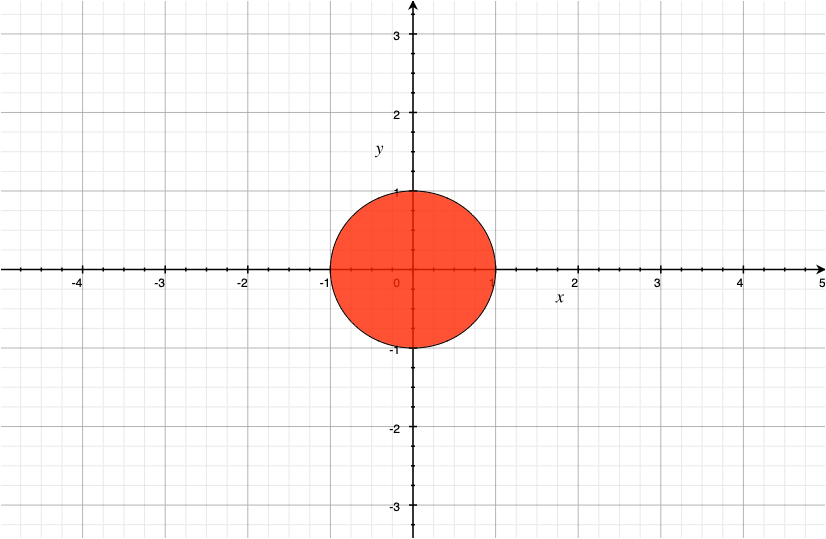
\includegraphics[width=0.7\textwidth]{Analisi2/figures/norma_euclidea.jpg}
    \caption{Grafico di $B(\uline 0, 1)=\{\uline x\in\mathbb R^2\; |\;\sqrt{(x_1-0)^2+(x_2-0)^2}<1\}$.}
    \label{fig:distanza_euclidea_r_1}
\end{figure}

\begin{figure}
    \centering
    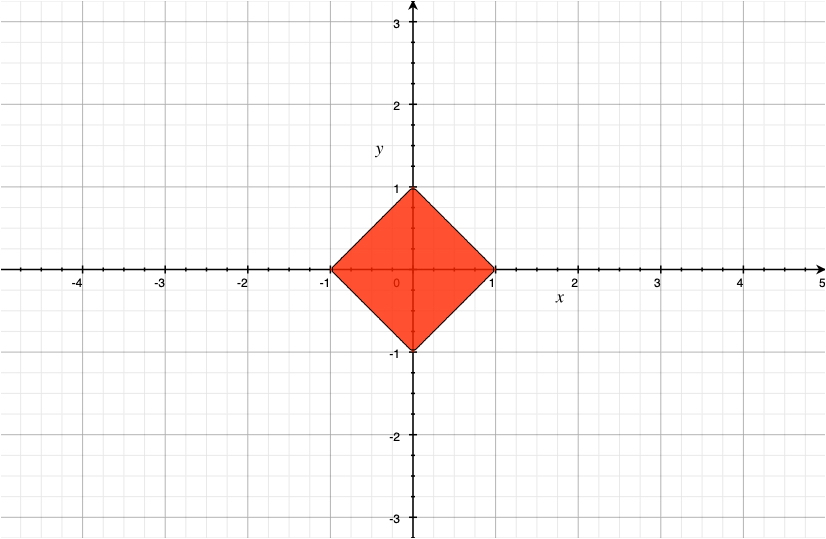
\includegraphics[width=0.7\textwidth]{Analisi2/figures/distanza_tassista.jpg}
    \caption{Grafico di $B(\uline 0, 1)=\{\uline x\in\mathbb R^2\; |\; |x_1-0|+|x_2-0|<1\}$.}
    \label{fig:distanza_tassista_r_1}
\end{figure}

È possibile ora trattare la topologia negli spazi metrici. Le nozioni che saranno date valgono per qualsiasi spazio metrico del tipo $(X,d)$. Per visualizzare i risultati sarà utilizzato $R^n$, con $n=2$ e $d=||\cdot||_2$ (ovvero dove gli intorni sferici sono dischi aperti).

\paragraph{N.B.:} Dato uno spazio metrico $(X,d)$ ed un suo \gls{sottospazio}, allora punto esterno, interno, di frontiera di un sottospazio, spazio aperto e chiuso definiscono la topologia dello spazio.

Vogliamo definire il concetto di limitatezza di un sottospazio metrico. Definendo le Proprietà \ref{prop:successione_convergente_Rn} delle successioni convergenti in $\mathbb R^n$ è stata trattata la limitatezza di una successione continua tramite la distanza. Una successione è un sottoinsieme di $\mathbb R^n$, quindi il concetto può essere generalizzato ad un sottospazio vettoriale $A$ di $X$.

Dati $(X,d)$ e $A\subset X$ (sottospazio di $X$), $x_0\in X,\, r>0$ e $B(\uline x_0, r)=\{x\in X|\, d(x_0,x)<r\}\subset X$, sono date le seguenti definizioni.

\begin{definition} [Sottospazio limitato]\footnote{Slide 7 PDF 8.}
    $A$ è detto limitato se esiste una palla aperta (in $X$) che lo contiene, cioe':
    \begin{equation*}
        \exists r>0,\exists x_0\in X\colon A\subset B(x_0,r).
    \end{equation*}
\end{definition}

Questa definizione riconduce alla limitatezza delle successioni.

\begin{definition}[Punto interno]\footnote{Slide 7 PDF 8.}
    $x_0\in X$ si dice interno ad $A\subset X$ se
    \begin{enumerate}
        \item $x_0\in A$, e
        \item $\exists r>0$ tc $B(x_0, r)\subset A$ \footnote{Ovvero esiste almeno un sottoinsieme sferico di $x_0$ contenuto in $A$.}.
    \end{enumerate}
\end{definition}

\begin{definition}[Punti interni ad $A$]
    I punti interni allo spazio vettoriale $A$ è indicato con $\mathring A$.
\end{definition}

\begin{definition}[Punto esterno]
    $\uline x_0\in X$ si dice punto esterno $A$ se
    \begin{enumerate}
        \item $\uline x_0\notin A$, e
        \item $\exists r>0\; B(\uline x_0, r)\cap A\neq 0$ \footnote{Ovvero: esiste intorno sferico di centro $x_0$ del tutto disgiunto ad $A$.}.
    \end{enumerate}
\end{definition}

\begin{definition}[Punto di frontiera]
    $\uline x_0\in A$ si dice punto di frontiera di $A$ se
    \begin{equation*}
        \exists r>0 \colon B(x_0,r)\cap A \cap A^C \neq 0,
    \end{equation*}
    ovvero se è non è né esterno né interno.
\end{definition}

\paragraph{Notazione punti di frontiera} L'insieme dei punti di frontiera di $A$ è denotato con $\partial A$.

Quindi $x_0$ è un punto di frontiera di $A$ (ovvero $x_0\in\partial A$) se ogni intorno di $x_0$ contiene punti interni ed esterni ad $A$.

\begin{definition}[Insieme aperto]\label{def:insieme_aperto}
    $A$ di dice aperto se $A=\emptyset$, oppure se ogni suo punto è interno ad $A$ (ovvero per ogni punto di $A$ esiste un suo intorno sferico contenuto in $A$).
\end{definition}

\begin{definition}[Insieme chiuso]\footnote{Definizione alternativa libro: $C\subset\mathbb R^n$ si dice chiuso se $A=\mathbb R^n\backslash C$ è aperto.}
    $C$ si dice chiuso se contiene tutti i suoi punti di frontiera, ovvero $\partial C\subset C$.
\end{definition}

\paragraph{N.B.:}\footnote{Slide 2 PDF 9.} Gli insiemi vuoi e $\mathbb R^n$ sono contemporaneamente aperti e chiusi perché entrambi sottoinsiemi di se stessi (inteso come $\emptyset\subseteq\emptyset,\, \mathbb R^n\subseteq\mathbb R^n$). Inoltre, un insieme aperto ha come complementare un insieme chiuso.

\paragraph{N.B.:} Esistono insiemi in $\mathbb R^n$ che non sono né aperti né chiusi.

\begin{definition}[Insieme complementare]\footnote{Definizione non data.}
    Dato $A\subset\mathbb R^n$ insieme aperto, l'insieme complementare di $A$ e'
    \begin{equation*}
        A^C=\{\uline x\in\mathbb R^n\;|\; x\notin A\}.
    \end{equation*}
\end{definition}

\textbf{Considerando lo spazio metrico $(\mathbb R^2, d)$ sono dati esempi in $\mathbb R^2$ di insiemi.}
\begin{example}\footnote{Slide 9 PDF 8.}
    Sia $A_1=\{(x,y)\in\mathbb R^2|x^2+y^2<9\}\subset\mathbb R^2$. $A_1$ è un intorno del cerchio di centro origine e raggio $r=3$. Inoltre $A_1$ è limitato ed aperto e $\partial A_1=\{(x,y)\in\mathbb R^2|x^2+y^2=9\}$. Vedere Figura \ref{fig:A_1_esempio}.
\end{example}

\begin{example}\footnote{Slide 9 PDF 8.}
    Sia $A_2=\{(x, y)\in\mathbb R^2\colon x\neq y^2\}\subset\mathbb R^2$. $A_2$ sono tutti i punti che non sono sulla parabola. $A_2$ non è limitato ed è aperto. $\partial A_2=\{(x,y)\in\mathbb R^2\colon x=y^2\}$. Vedere Figura \ref{fig:A_2_esempio}.
\end{example}

\begin{figure}
    \centering
    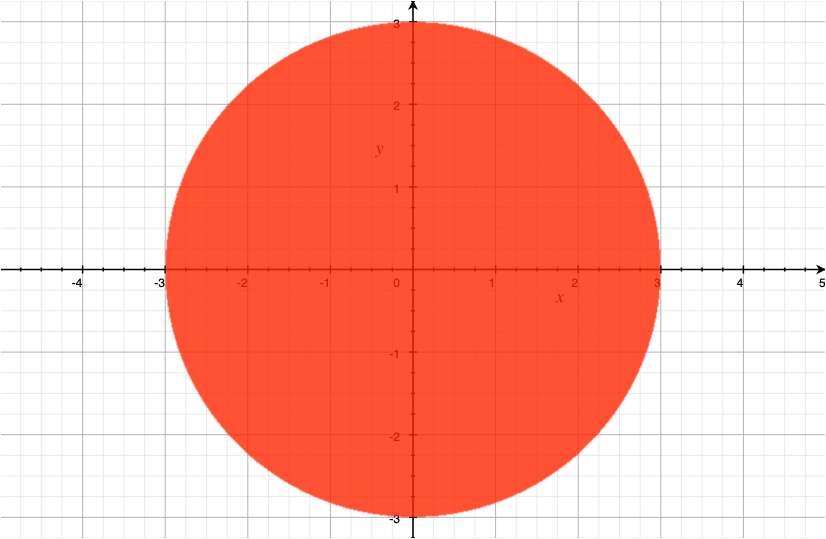
\includegraphics[width=0.7\textwidth]{Analisi2/figures/A1.jpg}
    \caption{Grafico di $A_1=\{(x,y)\in\mathbb R^2|x^2+y^2<9\}$.}
    \label{fig:A_1_esempio}
\end{figure}

\begin{figure}
    \centering
    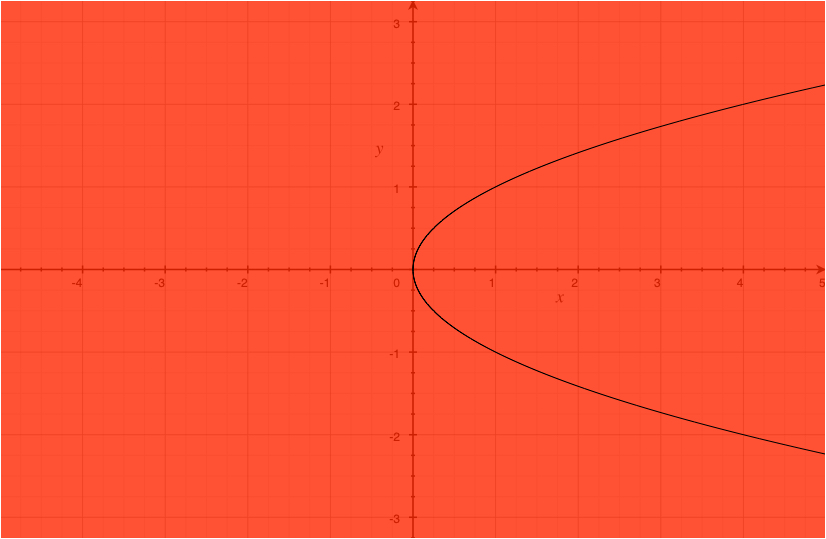
\includegraphics[width=0.7\textwidth]{Analisi2/figures/A2.jpg}
    \caption{Grafico di $A_2=\{(x, y)\in\mathbb R^2\colon x\neq y^2\}$.}
    \label{fig:A_2_esempio}
\end{figure}

\begin{example}\footnote{Slide 10 PDF 8. Questo esempio estende il Teorema \ref{th:esistenza_degli_zeri} degli zeri.}
    Sia $A_3=\{(x,y)\in\mathbb R^2\colon x+y+2\leq 0\}$. L'insieme è formato dai punti che stanno sotto alla funzione $\varphi:y=-x-2$. $A_3$ non è limitato ma chiuso (i punti di frontiera sono la retta). \footnotemark
\end{example}

\footnotetext{Vale il Teorema \ref{th:esistenza_degli_zeri} degli zeri perché gli zeri per la funzione di due variabili. Tale funzione divide in due sottoinsiemi connessi, cioe': il segno delle sottoregioni è costante perché sotto la retta gli elementi hanno segno negativo e sopra positivo. Cosa di dubbia utilità detta dalla prof: Per trovare quale sono i punti in $A_3$ è preso un punto comodo, ad esempio $(-3,0)$ e si sostituisce nella disequazione, determinando così la regione di interesse.}

\begin{definition}[Punto di accumulazione]\footnote{Slide 1 PDF 9.}
    Sia $A\subseteq\mathbb R^n$. $\uline x_0\in\mathbb R^n$ si dice punto di accumulazione per $A$ se \footnote{Comunque mi muovo vicino ad $\uline x_0$ trovo un punto in $A$.}
    \begin{equation*}
        B(\uline x_0, r)\cap (A\backslash\{x_0\})\neq\emptyset.
    \end{equation*}
\end{definition}

\begin{remark}
    Dato $A$ aperto, tutti i punti in $\mathring A$ sono punti di accumulazione.
\end{remark}

\paragraph{N.B.:} I punti di frontiera $\partial A$ possono essere o meno punti di accumulazione di $A$. I punti esterni non sono di accumulazione di $A$.

\begin{definition}[Punto isolato]\footnote{Slide 1 PDF 9.}
    Ogni punto di frontiera in $\partial A$ che non è di accumulazione è detto isolato.
\end{definition}

\paragraph{N.B.:} Non è difficile dimostrare che $\uline x_0$ sia un punto di accumulazione di $A\subseteq\mathbb R^n$ (tramite la definizione stessa di punto di accumulazione). $\uline x_0$ è un punto di accumulazione di $A$ s.se \footnote{Dato l'intorno sferico di centro $\uline x_0$ e raggio qualsiasi si trovano punti in $A$ vicino a $\uline x_0$ nell'intorno sferico. Ovvero: $\uline x_0$ è punto di accumulazione per $A$ s.se diventa quanto scritto dopo la nota.} $\uline x_0$ è il limite di una successione di elementi di $A$ tutti diversi da $x_0$.

\begin{example}\label{ex:norma_in_(1,2)}\footnote{Slide 2 PDF 9.}
    Determinare i punti di accumulazione e quelli di frontiera nel seguente insieme e stabilire se tale insieme è aperto o chiuso.
    \begin{equation*}
        A=\{\uline x\in\mathbb R\;|\; 1<||\uline x||<2\}.
    \end{equation*}
    $\partial A$ è composto dai punti $\uline x$ tc $||\uline x||=1$ e $||\uline x||=2$, ovvero i punti di circonferenza interna ed esterna.\\
    $A$ è un insieme aperto, quindi gli elementi di $\mathring A$ sono punti di accumulazione. Pertanto, $\partial A=\gamma_1\cup\gamma_2$ è l'insieme dei punti di accumulazione.\\
    Vedere Figura \ref{fig:esempio_punti_accumulazione}.
    \begin{figure}
    \centering
    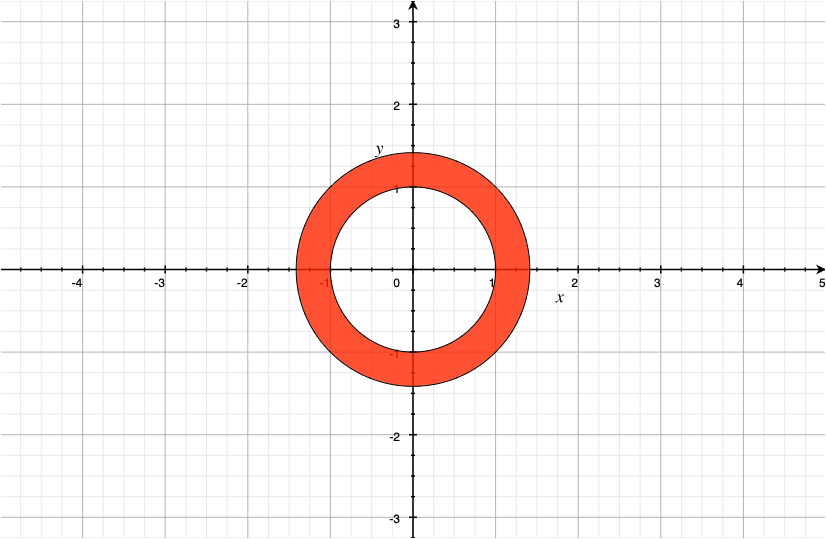
\includegraphics[width=0.5\textwidth]{Analisi2/figures/x2plusy2.jpg}
    \caption{Grafico di $A=\{\uline x\in\mathbb R\;|\; 1<||\uline x||<2\}$.}\label{fig:esempio_punti_accumulazione}
    \end{figure}
\end{example}

\begin{definition}[Chiusura di un insieme]\footnote{Slide 3 PDF 9.}
    La chiusura di $A\subseteq\mathbb R^2$ è denotata da $\bar A\, (\subset\mathbb R^n)$ ed è l'unione di $A$ con i suoi punti di accumulazione.
\end{definition}

\paragraph{N.B.:} $\bar A$ ha le seguenti caratteristiche:
\begin{enumerate}
    \item è un insieme chiuso.
    \item è il più piccolo chiuso che contiene $A$. È possibile dimostrare che $A\in\bar A$ e se $\Bar A=A$ allora $A$ è chiuso.
    \item $\bar A=A\cup\partial A$.
\end{enumerate}

In Analisi 1 una funzione è definita su un dominio (sottoinsieme di $\mathbb R$), ovvero è definita su un intervallo sottoinsiemi di $\mathbb R$. Un intervallo è fatto da un pezzo solo. Anche in Analisi 2 le funzioni sono definite su domini e sono del tipo
\begin{equation*}
    f\colon X\subseteq\mathbb R^n\rightarrow\mathbb R.
\end{equation*}

\begin{definition}[Dominio]\footnote{Slide 3 PDF 9.}
    Un dominio $D$ in $\mathbb R^n$ è la chiusura di un aperto $A\subset\mathbb R^n$, ovvero:
    \begin{equation}\label{eq:dominio_R_n}
        D=A\cup\partial A.
    \end{equation}
\end{definition}

\paragraph{N.B.:} Nell'Esempio \ref{ex:norma_in_(1,2)} il dominio è $D=\{\uline x\in\mathbb R^n\,;\, 1\leq||\uline x||\leq 2$\}, il quale è un insieme chiuso.

\begin{remark}\footnote{Slide 6 PDF 11.}
    Un dominio è un insieme massimale (rispetto all'inclusione su $\mathbb R^n$), ovvero un sottoinsieme di $\mathbb R^n$ massimo nel quale la funzione è ben definita.
\end{remark}

\begin{example}
    Una sfera chiusa contenuta in $\mathbb R^n$ è un dominio. Una sfera chiusa unito ad un punto isolato (esterno) non è un domino.
\end{example}

\subsection{Limite e continuità}
È stato trattato quanto precede sui punti di accumulazione per introdurre il concetto di limite in $\mathbb R^n$, quindi per funzioni di più variabili, con valori in $\mathbb R$. Inoltre, tramite il concetto di limite è possibile introdurre il concetto di continuità di una funzione.

\begin{definition}[Limite di funzione]\label{def:limite_funzione_piu_variabili}\footnote{Slide 4 PDF 9.}
    Data
    \begin{equation*}
        \begin{aligned}
            f\colon A\subseteq\mathbb R^n & \rightarrow \mathbb R\\
            \uline x &\mapsto f(\uline x)
        \end{aligned}
    \end{equation*}
    e sia $\uline x_0=(x_0^1,\hdots,x_0^n)\in\mathbb R^n$ un punto di accumulazione per $A$. Si dice che $f$ tende a $\ell\in$\gls{Rext}$=\mathbb R\cup\{\pm\infty\}$ per $\uline x$ che tende a $\uline x_0$ e si scrive
    \begin{equation}\label{eq:limite_funzione_piu_variabili}
        \lim_{\uline x\rightarrow\uline x_0}f(\uline x)=\ell \quad\text{ovvero}\quad f(\uline x)\overset{\footnotemark}{\underset{\uline x\rightarrow\uline x_0}{\longrightarrow}}\ell
    \end{equation}
    \footnotemark se per ogni intorno $U\subset\overline{\mathbb R}$ di $\ell$ esiste un intorno sferico di $\uline x_0$, ovvero:
    \begin{equation*}
        \exists r>0,\, I(\uline x_0, r)=B(\uline x_0,r)\subset\mathbb R^2 \text{ tc } f(\uline x)\in U\quad \forall\uline x\in I(\uline x_0,r)\cap(A\backslash\{\uline x_0\}).
    \end{equation*}
\end{definition}

\addtocounter{footnote}{-1}
\footnotetext{$f(\uline x)\underset{\uline x\rightarrow\uline x_0}{\longrightarrow}\ell$ significa che $f(\uline x)$ appartiene all'intorno di $\ell$ non appena $\uline x$ è nell'intorno sferico di $\uline x_0$. Stessa definizione di Analisi 1.}

\stepcounter{footnote}
\footnotetext{Dato che $\ell\in\overline{\mathbb R}$, è possibile parlare di intorni di infinito, ovvero semirette finite del tipo $(n,+\infty)$ o $(-\infty, n)$.}

\paragraph{N.B.:} Il limite di funzione appena definito è una operazione definita su $\overline{\mathbb R}$ e quindi $\ell$ può essere un numero reale o $\pm\infty$.\\
La Definizione \ref{def:limite_funzione_piu_variabili} di limite di funzione è la stessa definizione di limite di Analisi 1, si distingue per $\pm\infty$. Quando $\ell=\pm\infty$ significa che esiste $M$ tale che $f$ da un certo punto in poi è maggiore di $M$, quindi $f$ ha valori appartenenti alla semiretta $(M,+\infty)$ (intorno di $+\infty$). Per avere una notazione compatta è utilizzato un certo intorno, come sopra.

La Definizione \ref{def:limite_funzione_piu_variabili} di limite di funzione è equivalente alle Definizioni \ref{def:limite_epsilon_delta_convergente_piu_variabili} e \ref{def:limite_epsilon_delta_divergente_piu_variabili} di limite convergente e divergente $\varepsilon$-$\delta$ seguenti.

\begin{definition}[Limite finito $\varepsilon$-$\delta$]\label{def:limite_epsilon_delta_convergente_piu_variabili}\footnote{Slide 4 PDF 9.}
    \begin{equation*}
        \lim_{\uline x\rightarrow\uline x_0}f(\uline x)=\ell\in\mathbb R
    \end{equation*}
    è finito se
    \begin{equation}
        \forall\varepsilon>0\;\exists\delta>0\quad\text{tc}\quad \underbrace{\overbrace{|f(\uline x)-\ell|}^{d(f(\uline x,\ell))\in\mathbb R}<\varepsilon}_{\footnotemark}\quad \underbrace{\forall\uline x\in(A\backslash\{\uline x_0\}) \text{ con } ||\uline x-\uline x_0||<\delta \text{ e } \uline x\in B(\uline x_0,\delta)}_{\footnotemark}.
    \end{equation}
\end{definition}

\addtocounter{footnote}{-1}
\footnotetext{Equivale a $\underbrace{\ell-\varepsilon<f(\uline x)<\ell +\varepsilon\equiv B(\ell, \varepsilon)}_{\subset\mathbb R}\ni f(\uline x)$.}

\stepcounter{footnote}
\footnotetext{Può essere espresso come segue: $\forall\uline x\in A$ con $0<||\uline x - \uline x_0||<\delta$. La norma deve essere maggiore stretta di 0 perché è necessario che $\uline x\neq \uline x_0$.}

In modo analogo sono definiti i limiti divergenti.
\begin{definition}[Limite divergente $\varepsilon$-$\delta$]\label{def:limite_epsilon_delta_divergente_piu_variabili}\footnote{Libro PG 42.}
    \begin{equation*}
        \lim_{\uline x\rightarrow\uline x_0}f(\uline x)=\pm\infty
    \end{equation*}
    è divergente a $\pm\infty$ se
    \begin{equation}\label{eq:limite_epsilon_delta_divergente_piu_variabili}
        \forall M>0\;\exists\delta>0\quad\text{tc}\quad f(\uline x)>M \quad \forall\uline x\in(A\backslash\{\uline x_0\}) \text{ con } ||\uline x-\uline x_0||<\delta \text{ e } \uline x\in B(\uline x_0,\delta).
    \end{equation}
\end{definition}

Il limite di una funzione segue la stessa algebra e le stesse regole che in Analisi 1.
\begin{property}[Proprietà limite di funzione]\footnote{Slide 5 PDF 9.}
    Il limite di funzione definito come (\ref{eq:limite_funzione_piu_variabili}) ha le seguenti proprietà:
    \begin{enumerate}
        \item se esiste è unico,
        \item il limite di somma e prodotto di funzioni (reali in più variabili) sono uguali alla somma e prodotto di limiti (se esistono),
        \item il limite del rapporto (di quoziente) è uguale al rapporto (quoziente) fra i limiti (se ben definiti, ovvero denominatore diverso da 0 e definita l'operazione di quoziente).
        \item $\lim_{\uline x\rightarrow\uline x_0}c\cdot f(\uline x)=c\cdot\lim_{\uline x\rightarrow \uline x_0}f(\uline x)$
    \end{enumerate}
\end{property}

\paragraph{N.B.:} Somma (la sottrazione è come somma cambiata di segno: $x-y=x+(-1) y$) e prodotto di funzione sono intese come algebriche.

\paragraph{Suggerimento:} prima di calcolare un limite verificare se esiste.

\begin{example}\footnote{Slide 5 PDF 9.}
    Sia
    \begin{equation*}
        f(x,y)=\frac{x^2}{\sqrt{x^2+y^2}}\colon A=\mathbb R^2\backslash\{(0,0)\}\rightarrow\mathbb R.
    \end{equation*}
    $\uline 0\notin A$ è un punto di accumulazione per $A$.
    \footnote{Vogliamo mostrare, tramite la definizione di limite, cosa accade vicino l'origine della funzione.} Mostriamo che
    \begin{equation*}
        \lim_{(x,y)\rightarrow(0,0)}f(x,y)=0.\footnotemark
    \end{equation*}
    \footnotetext{Quindi è necessario dimostrare che comunque preso un intorno in $\mathbb R^2$ di $\uline 0$ esiste un intorno di raggio $\delta$ nell'origine di punti di $A$ diversi da $(0,0)$ per cui $f$ è nell'intorno di $\uline 0$ non appena le coppie $(x,y)\in I_\delta((0,0))$.}
    È necessario dimostrare quindi che
    \begin{equation*}
        \lim_{(x,y)\rightarrow(0,0)}\frac{x^2}{\sqrt{x^2+y^2}}=0
    \end{equation*}
    ovvero (tramite (\ref{eq:limite_epsilon_delta_divergente_piu_variabili}))
    \begin{equation*}
        \forall\varepsilon>0\,\exists\delta=\delta_\varepsilon>0,\, \underbrace{|f(x,y)-0|<\varepsilon}_{d(f(x,y),\uline 0)\in\mathbb R}\quad \forall(x,y)\in A \text{ con } \underbrace{0<\sqrt{x^2+y^2}<\delta}_{\footnotemark}.
    \end{equation*}
    \footnotetext{$B(\uline 0, \delta)=\{\uline x\in\mathbb R^2\,|\, d(\uline x,\uline 0)=||\uline x-\uline 0||<\delta\}$.}
    \footnote{È necessario verificare che $0<\sqrt{x^2+y^2}<\delta$.} È possibile osservare che
    \begin{equation*}
        0\leq\underbrace{\frac{x^2}{\sqrt{x^2+y^2}}\leq\frac{x^2+y^2}{\sqrt{x^2+y^2}}=\sqrt{x^2+y^2}}_{\footnotemark},
    \end{equation*}
    dimostrando che
    \begin{equation}\label{eq:esempio_limite}
        0\leq f(x,y)\leq \sqrt{x^2+y^2}=\delta=\delta_\varepsilon\quad \forall(x,y)\in A
    \end{equation}
    e dunque
    \begin{equation*}
        \forall\varepsilon>0\;\exists\delta = \sqrt{x^2+y^2}\quad \text{ tc }\quad 0\leq f(x,y)\leq\varepsilon\quad\forall(x,y)\neq(0,0)\quad\text{ tc }\quad \sqrt{x^2+y^2}=\delta_\varepsilon<\varepsilon.
    \end{equation*}
    Quindi, da (\ref{eq:esempio_limite}), $|f(x,y)-0|<\varepsilon$.
\end{example}
\footnotetext{Applicata maggiorazione con un'espressione con valore \gls{infinitesimo}, ovvero $\sqrt{x^2+y^2}$. $\sqrt{x^2+y^2}$ è un infinitesimo ed è uguale a $\delta$ (della Definizione \ref{def:limite_epsilon_delta_convergente_piu_variabili} di limite finito $\varepsilon$-$\delta$).}

Il problema principale dei limiti è dimostrare l'esistenza. Le funzioni in più variabili tendono a non avere limite. Ci sono teoremi per dimostrare che il limite di una funzione in più variabili non esiste. Inoltre, per le funzioni in più variabili, può essere utile trasformare le coordinate cartesiane in coordinate polari per semplificare il calcolo dei limiti.

\begin{example}\footnote{Slide 7 PDF 9.}
    Mostrare che 
    \begin{equation*}
        \lim_{(x,y)\rightarrow(0,0)}\frac{x}{\sqrt{x^2+y^2}}
    \end{equation*}
    non esiste. $f=\frac{x}{\sqrt{x^2+y^2}}\colon A=\mathbb R^2\backslash\{\uline 0\}\rightarrow\mathbb R$.\\
    \footnotemark È necessario mostrare cosa accade in un intorno di centro $(0,0)$ e raggio $r=\delta$. È possibile muoversi vicino a $(0,0)$ sull'asse $y$ (quindi con $x=0$). Dunque è considerata $f(0,y)=0$ al variare di $y$ (quindi il candidato dovrebbe essere 0).\\
    Muovendosi sull'asse $x$, con $y=0$, la funzione assume i seguenti valori:
    \begin{equation}\label{eq:esempio_limiti_1}
        f(x,0)=\frac{x}{\sqrt{x^2}}=\frac{x}{|x|}=
        \begin{cases}
            1, & x>0,\\
            -1,& x>0.
        \end{cases}
    \end{equation}
    Quindi il limite non è unico: il valore del limite dipende dalla direzione con la quale $\uline x$ si avvicina a $(0,0)$. Ovvero $\nexists\lim_{(x,y)\rightarrow(0,0)}f(x,y)$.

    \begin{figure}
    \centering
    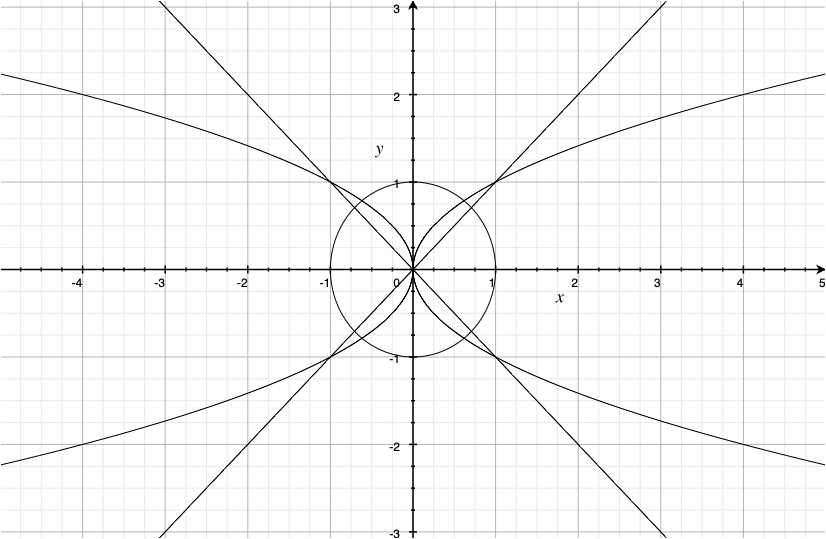
\includegraphics[width=0.5\textwidth]{Analisi2/figures/cammini_0,0.jpg}
    \caption{Grafico di alcuni possibili cammini che "portano" all'origine $(0,0)$.}\label{fig:cammini_0,0}
    \end{figure}
\end{example}

\footnotetext{$f$ è definita su tutto $\mathbb R^2$ tranne nell'origine. Vogliamo vedere cosa accade ad $f$ nell'origine tramite la definizione di limite. Muoversi in $\mathbb R$ (ovvero sul piano) nell'\gls{asse reale} vicino ad $x_0$ significa stare a sinistra o a destra di $x_0$ ma entro $\delta$. In $\mathbb R^2$ le direzioni sono infinite, quindi è possibile muoversi vicino ad $x_0$ in tutte le direzioni. Per semplicità è scelto un cammino semplice. Con cammino semplice si intende percorrere le assi $x,y$, le bisettrici, parabole, come in Figura \ref{fig:cammini_0,0}, o un qualsiasi altro degli infiniti cammini che portano all'origine. Quindi in $\mathbb R^2$ è più complesso che in Analisi 1 calcolare il limite di una funzione.}

\paragraph{Deduzioni dall'esempio:} L'esistenza del limite non può dipendere da come ci si avvicina al punto "problematico", ovvero il limite deve essere lo stesso indipendentemente dalla direzione di avvicinamento di $(x,y)$ al punto $(x_0, y_0)$ e non dipendere dal modo (ovvero dalla direzione di avvicinamento). Una direzione nel piano è un vettore modulo, ovvero $\uline x\in\mathbb R$ tale che $||\uline v||=1$ (in genere ad ogni vettore è associata una direzione sul piano).  In generale si parla di direzione quando un vettore è normalizzato, ovvero quando $||\uline x||=1$. Quindi, quando il limite esiste ed è unico significa che il limite non deve dipendere dalla direzione e/o dal cammino scelto con il quale il punto $P=(x,y)$ si avvicina al punto $P_0=(x_0,y_0)$.  Il cammino può essere inteso come una bisettrice, parabola, o qualsiasi alta curva come in Figura \ref{fig:cammini_0,0}. In altre parole ancora: trovati due cammini percorrendo il quali $P$ si avvicina a $P_0$, è possibile provare che se tendono a $P_0$ e danno limiti diversi allora il limite non esiste.

\paragraph{N.B.:} Potrebbe capitare che due cammini portino a due valori reali distinti (già questo permette di determinare che il limite non esiste).

\paragraph{N.B.:} Il punto "generico" di un limite di funzione in più variabili $\uline x=(x_0,x_1,\hdots, x_n)\in\mathbb R^n$ può essere denotato con $P$ ed il punto di accumulazione $\uline x_0=(x_0^1,x_0^2,\hdots, x_0^n)\in\mathbb R^n$ come $P_0$. Inoltre, data $f:A\subset\mathbb R^2\rightarrow\mathbb R$ con $(x_0,y_0)$ punto di accumulazione per $A$, per descrivere l'operazione di limite di funzione può essere utilizzata la notazione $P,\, P_0$ così risaltare il carattere geometrico della funzione (ad ogni coppia è associata un punto sul piano e viceversa per la corrispondenza biunivoca del piano cartesiano tra coppie ordinata e punti sul piano). Ovvero, dati $P=(x,y), P_0=(x_0,y_0)$,
\begin{equation*}
    \lim_{(x,y)\rightarrow(x_0,y_0)}f(x,y)=l\in\mathbb R \quad\text{equivale a}\quad \lim_{P\rightarrow P_0}f(P)=P_0.
\end{equation*}

La seguente proposizione permette di affermare quando un limite esiste (formalizzando quanto scritto sopra).

\begin{proposition}[Condizione necessaria per l'esistenza del limite]\footnote{Slide 8 PDF 9.}
    Sia $f\colon A\subset\mathbb R^2\rightarrow\mathbb R$ e $(x_0, y_0)$ punto di accumulazione per $A$. Se
    \begin{equation*}
        \lim_{(x,y)\rightarrow(x_0,y_0)} f(x,y)=\ell
    \end{equation*}
    allora $\forall C\subset A$ deve valere
    \begin{equation*}
        \lim_{C\ni(x,y)\rightarrow (x_0,y_0)}f(x, y)=\ell.
    \end{equation*}
\end{proposition}

\paragraph{N.B.:} trovare $n$ cammini che confermano che il limite è valido non significa che il limite esista. La Proposizione è una condizione necessaria ma non sufficiente.

\begin{remark}
    è possibile osservare che come condizione necessaria per l'esistenza del limite è spesso utilizzato il fatto che esistano, e che siano uguali fra loro, i limiti lungo le rette parallele agli assi coordinati di equazione $y=y_0\in\mathbb R$ e $x=x_0\in\mathbb R$ (costanti), ottenendo come condizione necessaria per l'esistenza
    \begin{equation*}
        \lim_{x\rightarrow x_0}f(x,y_0)=\ell=\lim_{y\rightarrow y_0}f(x_0, y).
    \end{equation*}
\end{remark}

\begin{exercise}[Per casa]\label{exercise:limite_non_esiste_casa}
    Mostrare che il seguente limite non esiste
    \begin{equation*}
        \lim_{(x,y)\rightarrow(0,0)}\frac{xy}{x^2+y^2}.
    \end{equation*}
    Consigli su come farlo: Prima provare cosa accade sugli assi coordinati. Seconda cosa provare qualche curva.\\
    \textbf{Svolgimento:}
    \begin{equation*}
        \lim_{\underset{x=y}{(x,y)\rightarrow(0,0)}}f(x,y)=\lim_{y\rightarrow 0}f(y,y)=\lim_{y\rightarrow 0}\frac{y\cdot y}{y^2+y^2}=\lim_{y\rightarrow 0}\frac{\cancel{y^2}}{2\cancel{y^2}}=\frac{1}{2}=\lim_{x\rightarrow 0}\frac{x\cdot x}{x^2+x^2}=\lim_{x\rightarrow 0}f(x,x)=\lim_{\underset{y=x}{(x,y)\rightarrow(0,0)}}f(x,y).
    \end{equation*}
    \begin{equation*}
       \lim_{\underset{y=x^2}{(x,y)\rightarrow(0,0)}}f(x,y)=\lim_{x\rightarrow 0}\frac{x\cdot x^2}{x^2+(x^2)^2}=\lim_{x\rightarrow 0}\frac{x^{\cancel{3}}}{\cancel{x^2}(1+x^2)}=0.
    \end{equation*}
    Dato che $0\neq \frac{1}{2}$, il limite non esiste.
\end{exercise}

\begin{definition}[Continuità di funzione]\footnote{Slide 1 PDF 10.}\label{def:continuita_funzione_n_variabili}
    Sia $f\colon A\subseteq\mathbb R^n\rightarrow\mathbb R$ e (supposto $n=2$) sia $P_0=(x_0,y_0)\in A$. Se $P_0$ è punto di accumulazione per $A$, $f$ si dice continua in $P_0$ se
    \begin{equation}\label{eq:limite_continuita}
        \lim_{(x,y)\rightarrow(x_0,y_0)}f(x,y)=f(x_0,y_0)\quad \left(\text{per } n>2\; \lim_{\uline x\rightarrow\uline x_0}f(\uline x)=f(\uline x_0)\right).
    \end{equation}
    Se $P_0$ è un punto isolato per $A$ per convenzione si pone $f$ continua in tale punto.
\end{definition}

\begin{definition}[Funzione continua]\footnote{Slide 1 PDF 10.}
    Sia $f\colon A\subset\mathbb R^n\rightarrow\mathbb R$. $f$ si dice continua in $A$ se è continua in ogni punto di $A$.
\end{definition}

Per mostrare la continuità di una funzione in un punto è necessario quini mostrare quanto appena scritto.

\begin{example}\footnote{Slide 1 PDF 10.}
    Siano $f(x,y)=x$ e $g(x,y)=y$, quindi $f,g\colon A=\mathbb R^2\rightarrow\mathbb R$ (ovvero $f$ e $g$ sono funzioni continue in $A=\mathbb R^2$).\\
    Mostriamo che $f(x,y)$ è continua in $\forall P_0=(x_0,y_0)\in\mathbb R^2$. È necessario mostrare che
    \begin{equation*}
        \lim_{(x,y)\rightarrow(x_0,y_0)}f(x,y)=f(x_0,y_0)\in\mathbb R\; \text{(reale finito)}.
    \end{equation*}
    \footnote{È necessario che il limite di $f$ esiste ed è finito utilizzando la Definizione \ref{def:limite_epsilon_delta_convergente_piu_variabili} di limite finito.} Quindi è necessario mostrare che
    \begin{equation*}
        \forall\varepsilon>0\;\exists\delta=\delta(\varepsilon)>0 \text{ tc } |f(x,y)-f(x_0,y_0)|<\varepsilon \text{ se } (x,y)\in\mathbb R^2\cap B((x_0,y_0),\delta)\; \forall (x,y)\in\mathbb R^2, \underbrace{\sqrt{(x-x_0)^2+(y-y_0)^2}}_{d(P,P_0)}<\delta.
    \end{equation*}
    (Quindi è necessario mostrare che) $\sqrt{(x-x_0)^2+(y-y_0)^2}<\delta\iff|\equalto{x}{f(x,y)}-x_0|<\varepsilon$.\\
    (È possibile scrivere in modo diverso $|\cdot|$)  $0\leq|x-x_0|\overset{\footnotemark}{=}\sqrt{(x-x_0)^2}\leq\sqrt{(x-x_0)^2+(y-y_0)^2}<\delta$, quindi la definizione vale in $\delta=\varepsilon$.\\
    (Analogo procedimento con $g(x,y)=y^2$.)
\end{example}
\footnotetext{Trasformazione in radice aritmetica di un numero non negativo.}

\paragraph{N.B.:} Per le funzioni in una variabile ci sono opportuni teoremi sulle operazioni algebriche e sulla continuità. Per le funzioni in più variabili valgono gli stessi risultati con opportune considerazioni. Pertanto, è necessario estendere tali teoremi su domini in $\mathbb R^n$. Concetti che non coincidono con fra funzioni in una variabile ed in più variabili sono differenziabilità e derivabilità:
\begin{itemize}
    \item Per le funzioni in una variabile coincidono,
    \item Per le funzioni in più variabili il concetto di derivabilità è generalizzato nel concetto di differenziabilità. La differenziabilità è una proprietà più forte della derivabilità. La derivabilità in $\mathbb R^n$ non ha le stesse proprietà che in $\mathbb R$.
\end{itemize}

Il prossimo Teorema riguarda l'algebra delle funzioni in più variabili.
\begin{theorem}\label{th:algebra_funzioni_piu_variabili}\footnote{Slide 2 PDF 10.}
    Siano $f$ e $g$ funzioni di più variabili a valori reali continue (negli opportuni domini o in un punto), allora
    \begin{enumerate}
        \item $f\pm g$ (somma algebrica) e $f\cdot g$ sono continue (negli opportuni domini),
        \item (quoziente) se $g\neq 0$ allora $\frac{f}{g}$ è continua,
        \item (Legge di esponenziazione) se $g>0$ allora $f^g$ è continua,
        \item la funzione composta $g\circ f$ è continua dove è definita.
    \end{enumerate}
\end{theorem}

\begin{remark}\footnote{Slide 3 PDF 10.}
    Sia $f\colon A\subseteq\mathbb R^n\rightarrow\mathbb R$ e $g:J\subseteq\mathbb R\rightarrow\mathbb R$, allora $g\circ f\colon \mathbb\rightarrow\mathbb R$ segue il seguente processo
    \begin{equation*}
        \uline x\mapsto \underset{\underset{\mathbb R,\, D(g)}{\vertin}}{f(\uline x)}\mapsto g(f(\uline x)).
    \end{equation*}
    Per poter valutare $g\circ f$, $f(x)$ deve appartenere al dominio di $g$, ovvero $Imm(f)=f(A)\subseteq D(g)\subseteq\mathbb R$.
\end{remark}

\paragraph{N.B.:} Utilizzando il precedente Teorema \ref{th:algebra_funzioni_piu_variabili} è possibile affermare che le seguenti funzioni elementari sono continue:
\begin{itemize}
    \item Polinomi in più variabili,
    \item Funzioni razionali (quoziente di polinomi), dove il denominatore è diverso da 0 (ovvero le funzioni sono ben definite),
    \item Esponenziali in più variabili (esempio: $e^{x^2+y^2}$)
    \item Funzioni trigonometriche e loro inverse.
\end{itemize}
Inoltre è possibile affermare che tutte le funzioni elementari combinate con somme algebriche, prodotti ed esponenziazioni sono continue.

\begin{example}
    Data la funzione (razionale in due variabili)
    \begin{equation*}
        f(x,y)=\frac{e^{\frac{x^2-y^3}{x^2+y^2}}}{\cos(y-x)},
    \end{equation*}
    determinare il suo insieme di definizione $A\subseteq\mathbb R^2$, disegnarlo e stabilire la metrica topologica.
    \begin{itemize}
        \item (Dominio)
        \begin{equation*}
            \begin{matrix}
                \boldsymbol A&=&\{(x,y)\in\mathbb R^2;x^2+y^2\neq 0,\; \cos(y-x)\neq 0\}\\
                &=&\{(x,y)\in\mathbb R^2;(x,y)\neq(0,0),\, y-x\neq \frac{\pi}{2}+k\pi,\, \forall k\in\mathbb Z\}\\
                &=&\boldsymbol{\{(x,y)\in\mathbb R^2;(x,y)\neq(0,0),\, y\neq x + \frac{\pi}{2}+k\pi,\, \forall k\in\mathbb Z\}}.
            \end{matrix}
        \end{equation*}
        \item (Disegno) Vedere Figura \ref{fig:esempio_dominio_analisi2}. [Il dominio è la parte in blu che non comprende le rette $y=x+\frac{\pi}{2}+k\pi$.]
        \item (Metrica topologica) Il dominio $A$ è l'unione di aperti e non è limitato.
    \end{itemize}
    \begin{figure}
    \centering
    
\includegraphics[width=0.5\textwidth]{Analisi2/figures/A_dom.jpg}
    \caption{Grafico di $A=\{(x,y)\in\mathbb R^2;(x,y)\neq(0,0),\, y\neq x + \frac{\pi}{2}+k\pi,\, \forall k\in\mathbb Z\}$.}\label{fig:esempio_dominio_analisi2}
    \end{figure}
\end{example}

\begin{example}\footnote{Slide 5 PDF 10.}
    Data la funzione
    \begin{equation*}
        f(x,y)=
        \begin{cases}
            \frac{e^{(x-1)+(y-1)}-1}{\sqrt{(x-1)^2+(y-1)^2}} &\text{se } (x,y)\neq (1,1),\\
            0 &\text{se } (x,y)=(1,1),
        \end{cases}
    \end{equation*}
    studiarne la continuità sul suo dominio di definizione.\\
    $f$ è definito su $\mathbb R^2$, ovvero: $f\colon\mathbb R^2\rightarrow\mathbb R$.\\
    \footnote{Studiare il problema significa studiare la continuità. Per le conseguenze del Teorema \ref{th:algebra_funzioni_piu_variabili}, $f$ è continua in ogni punto di $\mathbb R^2$ diverso da $(1,1)$ perché funzione quoziente. Per verificare la continuità è necessario che il limite di $f(x,y)$ per $(x,y)\rightarrow (1,1)$ converga a 0, ovvero quanto segue alla nota.} Affinché $f$ risulti continua in tutto $\mathbb R^2$ allora (deve esistere il limite e valere 0, ovvero)
    \begin{equation*}
        \lim_{(x,y)\rightarrow(1,1)} f(x,y)=\lim_{(x,y)\rightarrow(1,1)}\frac{e^{(x-1)+(y-1)}-1}{\sqrt{(x-1)^2+(y-1)^2}}=f(1,1)=0.
    \end{equation*}
    Studiamo dunque $\lim_{(x,y)\rightarrow(1,1)}f(x,y)$. \footnote{Ciò che è richiesto è di provare prima che il limite esista, che sia finito e che coincida con valore della funzione nel punto. In questo caso non può essere $\pm\infty$. Se il limite esiste ed ha un valore diverso da 0 nel punto $(1,1)$ ed è necessario rendere la funzione continua nel punto, allora è possibile ridefinire la funzione in quel punto con il valore del limite, come per Analisi 1.}\footnote{Il limite fa capire cosa accade vicino al punto $(1,1)$. È possibile decidere di muoversi lungo qualsiasi cammino per avvicinarsi al punto. Quindi è possibile muovesi lungo la retta verticale seguendo i punti $(x,y)\in\{1\}\times\mathbb R\backslash\{1\}$ (come in Figura \ref{fig:esempio_f_1_y}, ovvero ciò che segue alla nota.)} Muovendosi lungo i $x=1$ con $y\neq 1$ è considerata
    \begin{equation*}
        f(1, y)=\frac{e^{y-1}-1}{\sqrt{(y-1)^2}}.
    \end{equation*}
    Quindi (con $y$ che tende ad 1 lungo la retta in Figura \ref{fig:esempio_f_1_y} dall'alto o dal basso)
    \begin{equation*}
        \lim_{\underset{x=1}{(x,y)\rightarrow(1,1)}}f(x,y)=\lim_{y\rightarrow 1}f(1,y)=\lim_{y\rightarrow 1}\frac{e^{y-1}-1}{\sqrt{(y-1)^2}}=\lim_{y\rightarrow 1}\frac{e^{y-1}-1}{(y-1)}\overset{\footnotemark}{=}
        \begin{cases}
            1 &\text{se } y>1\\
            -1 &\text{se } y<1
        \end{cases}
    \end{equation*}
    \footnotetext{Utilizzato il limite notevole $\lim_{t\rightarrow 0}\frac{e^t-1}{t}=1$. Tale limite è dovuto allo sviluppo di Taylor: $\lim_{t\rightarrow 0} e^t=1+t+o(t)$.}
    Quindi il limite non esiste e la funzione non è continua nel punto $(1,1)$. Ovvero: non vale la definizione di continuità.
    \begin{figure}
    \centering
    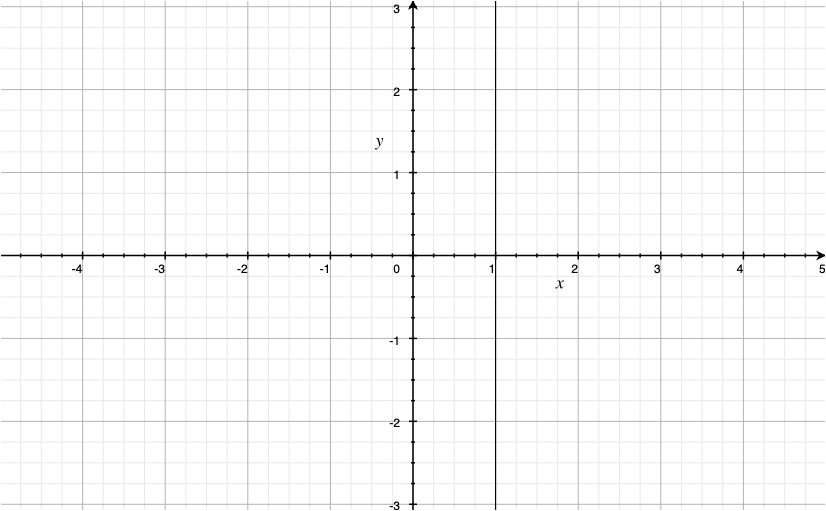
\includegraphics[width=0.5\textwidth]{Analisi2/figures/esempio_f_1_y.jpg}
    \caption{Grafico del cammino utilizzato per avvicinarsi al punto $(1,1)$.}\label{fig:esempio_f_1_y}
    \end{figure}
\end{example}

\paragraph{N.B.:} La definizione di continuità di una funzione stabilisce che la funzione $f(x,y)$, definita come $f\colon A\subset\mathbb R^2\rightarrow\mathbb R$, è continua in $(x_0, y_0)\in A$ se $\lim_{(x, y)\rightarrow (x_0,y_0)}f(x,y)=f(x_0, y_0)$. Questo non vale se il limite non esiste. La continuità vale se il limite esiste, è finito e coincide con il valore della funzione nel punto $(x_0, y_0)$. Può capitare che il limite non esista, sia infinito, oppure che esista finite ma con valore diverso da quello della funzione nel punto $(x_0, y_0)$. Quindi, per studiare la continuità è necessario studiare cosa accade nell'intorno del punto $(x_0, y_0)$.

\paragraph{N.B.:} Ogni esercizio che ha a che fare con i limiti può essere svolto nuovamente utilizzando le coordinate polari.

\begin{example}\footnote{Slide 7 PDF 10.}
    Calcolare l'esistenza del seguente limite:
    \begin{equation*}
        \lim_{(x,y)\rightarrow(0,0)}\frac{\sin^2(x)-\cos(y^2)}{x^2+y^2}.
    \end{equation*}
    Lungo l'asse $x$: ($y=0$ con $x\neq 0$)
    \begin{equation*}
        \lim_{\underset{y=0}{(x,y)\rightarrow(0,0)}}\frac{\sin^2(x)-\cos(y^2)}{x^2+y^2}=\lim_{x\rightarrow 0}\frac{\sin x^2}{x^2}=1.
    \end{equation*}
    Lungo l'asse $y$: ($y=0$ con $x\neq 0$)
    \begin{equation*}
        \lim_{y\rightarrow 0}\frac{-\sin y^2}{y^2}=-1
    \end{equation*}
    $-1\neq 1$, quindi non esiste limite unico.\\
    Nell'esempio sono stati trovati due cammini che danno luogo a limiti diversi. La condizione necessaria è che se la funzione ha limite $\ell$ allora per ogni cammino percorso per avvicinarsi al punto (qualsiasi sia la direzione) allora il limite deve valere $\ell$.
\end{example}

\begin{example}\footnote{Slide 8 PDF 10.}
    Verificare l'esistenza del seguente limite.
    \begin{equation*}
        \lim_{(x,y)\rightarrow(0,0)}\frac{\arctan(x+y)^2}{x^2}.
    \end{equation*}
    Lungo l'asse $x$: ($y=0$ con $x\neq 0$)
    \begin{equation*}
        \lim_{\underset{y=0}{(x,y)\rightarrow(0,0)}}f(x, y)= \lim_{x\rightarrow 0}\frac{\arctan(x^2)}{x^2}\overset{\footnotemark}{=}1.
    \end{equation*}
    \footnotetext{Utilizzato il limite notevole. Tramite la formula di Taylor: $\arctan t=0+\left.\frac{1}{1+t^2}\right|_{t=0}\cdot t +o(t)=t+o(t)$.}
    Lungo l'asse $y$: ($y=x$)
    \begin{equation*}
        \lim_{\underset{y=x}{(x,y)\rightarrow (0,0)}}f(x,y)=\lim_{x\rightarrow 0}f(x,x)=\lim_{x\rightarrow 0}\frac{\arctan(4x^2)}{x^2}=\lim_{x\rightarrow 0}\frac{\arctan(4x^2)}{4x^2}\cdot 4=4.
    \end{equation*}
    $4\neq 1$, quindi il limite non esiste.
\end{example}

\begin{example}\footnote{Slide 9 PDF 10.}
    \begin{equation*}
        \lim_{(x,y)\rightarrow(0,0)}\frac{y^3+x^5}{x^2+y^4}.
    \end{equation*}
    \footnote{Nominatore e denominatore sono polinomi con pesi diversi, quindi è necessario mettersi in una situazione di maggiore equilibrio.} Scegliendo come direzione di avvicinamento la parabola $x=y^2$, escludendo il punto $(0,0)$ perché $f$ non è definita, allora
    \begin{equation*}
        \lim_{\underset{x=y^2}{(x,y)\rightarrow(0,0)}}=\lim_{y\rightarrow 0}f(y^2, y)=\lim_{y\rightarrow 0}\frac{y^3+y^{10}}{y^4+y^4}=\lim_{y\rightarrow 0}\frac{\cancel{y^3}(1+y^7)}{2y^4\cancel{4}}=\pm\infty \text{ a seconda che }y\rightarrow 0^{\pm}.
    \end{equation*}
    Quindi il limite non esiste.
\end{example}

\begin{example}\footnote{Slide 10 PDF 10.}
    \begin{equation*}
        \lim_{(x,y)\rightarrow(0,0)}\frac{\sqrt[3]{x}y^{\frac{5}{3}}}{x^2+y^2}.
    \end{equation*}
    Globalmente il denominatore si comporta come una funzione di secondo grado perché gli esponenti sono razionali ed essendo un prodotto, il grado complessivo è determinato dalla somma dei due esponenti (5/3+1/3=2).\\
    Lungo l'asse $x$: ($y=0$ con $x\neq 0$) $f(x,0)=0$.\\
    Lungo l'asse $y$: ($x=0$ con $y\neq 0$) $f(0, y)=0$.
    Quindi il candidato al limite è 0 ed necessario verificare che lo sia.
    \begin{equation*}
        \lim_{\underset{y=x}{(x,y)\rightarrow(0,0)}}f(x,y)=\lim_{x\rightarrow 0}\frac{\sqrt[3]{x}x^{\frac{5}{3}}}{x^2+x^2}=\lim_{x\rightarrow 0}\frac{x^2}{2x^2}=\frac{1}{2}\neq 0,
    \end{equation*}
    quindi il limite non esiste.
\end{example}

\begin{example}\footnote{Slide 11 PDF 10.}
    \begin{equation*}
        \lim_{(x,y)\rightarrow(0,0)}\frac{e^{\sqrt{x^2+y^2}}-2}{x^2+y^2}=\left[\frac{-1}{0^+}\right]=-\infty.
    \end{equation*}
\end{example}

Se la funzione è continua nel punto allora è sufficiente calcolare la funzione in tale punto.
\begin{example}\footnote{Slide 11 PDF 10.}
    \begin{equation*}
        \lim_{(x,y)\rightarrow(0,0)}\frac{x^2-y^2}{x^2+y^2+77}=0.
    \end{equation*}
\end{example}

\begin{example}\footnote{Slide 11 PDF 10.}
    \begin{equation*}
        \lim_{(x,y)\rightarrow(0,0)}\frac{(x+y)^2}{x^2+y^2}.
    \end{equation*}
    Lungo l'asse $x$: ($y=0$ con $x\neq 0$)
    \begin{equation*}
        \lim_{\underset{y=0}{(x,y)\rightarrow(0,0)}}f(x,y)=\lim_{x\rightarrow 0}\frac{x^2}{x^2}=1, \text{ (candidato limite)}
    \end{equation*}
    Lungo la curva $y=x$:
    \begin{equation*}
        \lim_{\underset{y=x}{(x,y)\rightarrow(0,0)}}f(x,y)=\lim_{x\rightarrow 0}\frac{(x+y)^2}{x^2+x^2} = \frac{4x^2}{2x^2}=2\neq 1\quad\longrightarrow\quad\nexists\lim
    \end{equation*}
\end{example}

\paragraph{N.B.:} Non c'è un modo universale per affrontare i limiti, si cerca di utilizzare i teoremi e di capire se un limite esiste tramite il comportamento della funzione lungo opportuni cammini. Un metodo utile per il calcolo dei limiti è passare in coordinate polari, ovvero cambiare il sistema di coordinate da cartesiane a polari. [Off-topic: le coordinate sul piano dei complessi sono coordinate polari e ciò è utile per Fisica]. Nel piano cartesiano $R^2$ sono utilizzate le coppie ordinate per identificare i punti sul piano. In Figura \ref{fig:piano_coordinate_polari}, $x_P$ e $y_P$ sono le coordinate cartesiano che determinano univocamente $P=(x_P, y_P)$. è possibile determinare il punto $P$ tramite le due coordinate polari $\theta$ (un angolo \footnotemark) e $\rho$ (un raggio). Ciò significa che se sono note le misure $\overrightarrow{\rm OP}=\rho$ e $\theta$ è possibile determinare univocamente il punto $P$. \footnotetext{$\theta$ è l'angolo che il vettore $\overrightarrow{\rm OP}$ orientato positivamente forma con l'asse delle $X$.}

\begin{figure}
    \centering
    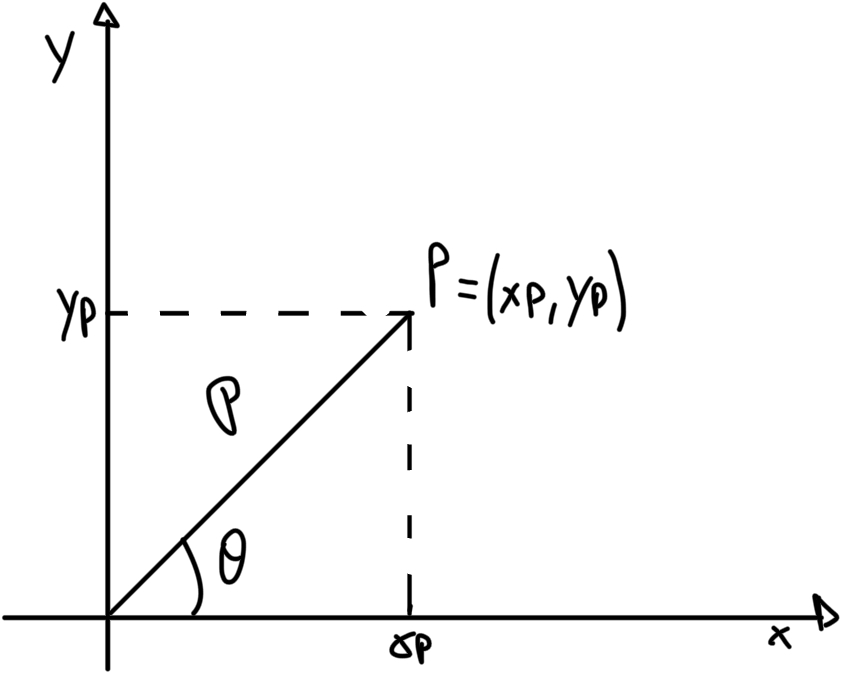
\includegraphics[width=0.5\textwidth]{Analisi2/figures/piano_coordinate_polari.jpeg}
    \caption{Grafico determinazione del punto $P=(x_P,y_P)$.}\label{fig:piano_coordinate_polari}
\end{figure}

\subsubsection{Coordinate polari}
\begin{definition}[Coordinate polari in $\mathbb R^2$ (non ufficiale)]\footnote{Slide 12, PDF 10.}\label{def:coordinate_polari}
    Siano $P=(x_P,y_P)\in\mathbb R^2$, $\rho=d(P,\uline 0)\in\mathbb R$ e $\theta$ l'angolo che $\overrightarrow{\rm OP}$ (orientato positivamente) forma con l'asse delle ascisse $x$. Data la circonferenza centrata nell'origine di raggio $\rho$, le coordinate polari di un punto $P$ nel piano $\mathbb R^2$ sono $(\rho, \theta)$, dove le coordinate polari sono determinate come
    \begin{equation}\label{eq:coordinate_polari_piano}
        \begin{cases}
            x_P=\rho\cos\theta\\
            y_P=\rho\sin\theta
        \end{cases}
    \end{equation}
\end{definition}

\begin{remark}\footnote{Slide 12 PDF 10.}
    Se $\rho\geq 0\Rightarrow \rho=\sqrt{x_P^2+y_P^2}$.
\end{remark}

\begin{remark}\footnote{Slide 12 PDF 10.}
    È possibile considerare la circonferenza trigonometrica centrata nell'origine di raggio $\rho$ come $\cos^2\theta+\sin^2\theta=\rho^2$. Quindi, l'ascissa è il coseno e l'ordinata il seno.
\end{remark}

\paragraph{N.B.:} Da (\ref{eq:coordinate_polari_piano}) è possibile dedurre che le coordinate cartesiane possono essere espresse in funzione delle coordinate polari. Quindi è necessario trovare $\theta$. Geometricamente $\theta$ è legata alla pendenza della retta $\overline{\rm OP}$ e la tangente di $\theta$ è il coefficiente angolare di $\overline{\rm OP}$. La pendenza può essere visualizzata come di quanto ci siamo alzati rispetto quanto ci siamo mossi, quindi $\frac{x}{y}$ (infatti $\tan x=\frac{\sin x}{\cos x}$). Quindi, se $\tan\theta$ è la pendenza di $\overline{\rm OP}$, 
\begin{equation*}
    \theta=\arctan\left(\frac{y_P}{x_P}\right).
\end{equation*}
Quindi la retta $\overline{\rm OP}$ può essere rappresentata come $y=mx$, con $m=\tan\theta$, dato che $\overline{\rm OP}$ passa per l'origine.

\begin{remark}[Non ufficiale]\footnote{Slide 13 PDF 10.}
    Le coordinate polari definite come nella Definizione \ref{def:coordinate_polari} sono centrate centrate in $(0,0)$. Le coordinate polari potrebbero essere traslate e centrate nel punto $(x_0,y_0)\neq(0,0)$ come in Figura \ref{fig:piano_coordinate_polari_centrate_x0_y0}, quindi è possibile generalizzare il caso (\ref{eq:coordinate_polari_piano}), ovvero: Nel caso in cui le coordinate siano centrate in $(x_0,y_0)$ allora $x$ e $y$ in coordinate cartesiano sono ottenute dalle coordinate polari seguendo le formule
    \begin{equation*}
        \begin{cases}
            x=x_0+\rho\cos\theta,\\
            y=y_0+\rho\sin\theta.
        \end{cases}
    \end{equation*}
\end{remark}
\begin{figure}
    \centering
    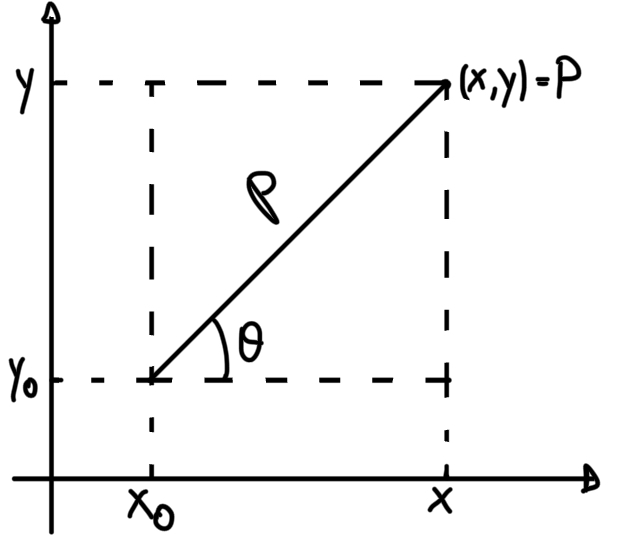
\includegraphics[width=0.5\textwidth]{Analisi2/figures/piano_coordinate_polari_centrate_x0_y0.jpg}
    \caption{Grafico determinazione del punto $P=(x,y)$.}\label{fig:piano_coordinate_polari_centrate_x0_y0}
\end{figure}

Il calcolo del limite di $f(P)$ quando $P\rightarrow P_0$ è possibile utilizzando le coordinate polari. Vale il seguente teorema.
\begin{theorem}\label{th:limite_funzione_due_variabili_coordinate_polari}\footnote{Slide 14 PDF 10.}
    Sia $f\colon D\subset\mathbb R^2\rightarrow\mathbb R$ e $P_0=(x_0,y_0)\in D$, allora
    \begin{equation}\label{eq:limite_tende_l_uniformemente_theta}
        \lim_{(x,y)\rightarrow(x_0,y_0)}f(x,y)=\ell\quad\iff\quad\lim_{\rho\rightarrow 0^+}\underbrace{f(x_0+\rho\cos\theta,y_0+\rho\sin\theta)}_{\footnotemark}=\ell\quad\text{$\underset{\footnotemark}{\text{uniformemente}}$ rispetto a $\theta$}.
    \end{equation}
\end{theorem}
\addtocounter{footnote}{-1}
\footnotetext{Dipende da $\rho$ e non da $\theta$ perché il limite deve valere uniformemente rispetto a $\theta$. È controllato quando $\rho\rightarrow0^+$ perché $\rho$ è una distanza, quindi $\rho\geq 0$.}

\stepcounter{footnote}
\footnotetext{Uniformemente rispetto a $\theta$ significa che il valore del limite cale comunque scelto $\theta$. È necessario ricordarsi che $\theta$ è un angolo, quindi di periodo $[0,2\pi]$ ed è sufficiente verificare cosa accade in tale intervallo e non su tutto $\mathbb R$.}

\paragraph{N.B.:} Nel caso del cambiamento di coordinate di una funzione, questa deve essere invertibile, quindi biettiva e per questo è necessario che il dominio della funzione sia un aperto (così ogni punto del dominio è associato ad un punto del codominio).

\paragraph{Conseguenze del Teorema \ref{th:limite_funzione_due_variabili_coordinate_polari}:} È valutato cosa accade quando $P=(x,y)\rightarrow P_0=(x_0,y_0)$. Con trasformazioni in coordinati polari del tipo
\begin{equation*}
    \begin{cases}
        x=x_0+\rho\cos\theta,\\
        y=y_0+\rho\sin\theta.
    \end{cases}
\end{equation*}
se $(x,y)\rightarrow(x_0,y_0)$ allora $\rho\cos\theta\rightarrow 0$ e $\rho\sin\theta\rightarrow 0$. Ciò vale per $\rho\rightarrow 0$ indipendentemente dal valore di $\theta\in(0,2\pi)$ ed è per questo che il limite (\ref{eq:limite_tende_l_uniformemente_theta}) vale uniformemente rispetto a $\theta$.\\
È utile passare in coordinate polari quando questo semplifica il calcolo dei limiti di funzioni radiali.

\paragraph{Cosa significa che $\boldsymbol{\lim_{\rho\rightarrow0^+}f(x_0+\rho\cos\theta, y_0+\rho\cos\theta)=\ell}$ (ovvero che vale (\ref{eq:limite_tende_l_uniformemente_theta}))?}

\begin{remark}[Non ufficiale]\footnote{Slide 1 PDF 11.}
    Affermare che vale il limite (\ref{eq:limite_tende_l_uniformemente_theta}) significa, tramite la Definizione \ref{def:limite_epsilon_delta} di limite $\varepsilon$-$\delta$, che
    \begin{equation}\label{eq:limite_coordinate_polari}
        \forall\varepsilon>0\; \exists\delta=\delta(\varepsilon)>0\quad\text{tc}\quad \underbrace{|f(x_0+\rho\cos\theta,y_0+\sin\theta)-\ell|}_{d(f(x_0, y_0),\ell)}<\varepsilon\quad\forall\rho\,(\rho\rightarrow0^+)\;0<\rho<\delta,\forall\theta\in(0,2\pi).
    \end{equation}
\end{remark}

\paragraph{N.B.:} Data l'Osservazione precedente, per mostrare che vale il limite della funzione $f$ per $(x,y)\rightarrow (x_0,y_0)$ è utilizzata un condizione semplice, ovvero è applicato il Teorema \ref{th:dei_carabinieri_2} dei Carabinieri: si cerca di maggiorare la quantità $|f(x_0+\rho\cos\theta,y_0+\sin\theta)-\ell|<\varepsilon$ in (\ref{eq:limite_coordinate_polari}) con una funzione che dipende solo dal raggio radiale, dove la funzione radiale è una maggiore uguale a 0 ed infinitesima (ovvero tende a 0 quando $\rho\rightarrow 0$).\\
Quindi, per mostrare che vale (\ref{eq:limite_tende_l_uniformemente_theta}) è sufficiente mostrare che (esiste) una funzione (radiale) $g=g(\rho)$ che dipende soltanto da $\rho$ con $g(\rho)\geq 0$ \footnote{Tale che $g$ sia maggiore di $|f(x_0+\rho\cos\theta,y_0+\sin\theta)-\ell|$ ed infinitesima quando $\rho\rightarrow 0^+$. Quindi è sufficiente far vedere che $g$ esiste, che sia maggiore uguale a 0 ed infinitesima quando $\rho\rightarrow 0^+$.} tale che
\begin{equation}\label{eq:maggiorazione_f_coordinate_polari}
    d(f,l)=|f(x_0+\rho\cos\theta,y_0+\sin\theta)-\ell|\leq g(\rho)\quad\text{e}\quad\lim_{\rho\rightarrow 0^+}g(\rho)=0.
\end{equation}
Quindi, (\ref{eq:maggiorazione_f_coordinate_polari}) significa che $d(f,\ell)$ è infinitesima non appena $0<\rho<\delta$, comunque scelta $\delta$.\\
Quindi, la tesi (\ref{eq:limite_tende_l_uniformemente_theta}) segue dal Teorema \ref{th:dei_carabinieri_2} dei Carabinieri (anche detto del confronto).

\paragraph{N.B.:} Potrebbe capitare che passando in coordinate polari il limite dipenda esplicitamente da $\theta$, ciò significa che il limite non esiste perché non vale uniformemente rispetto a $\theta$. Inoltre, se non riusciamo a dimostrare che esiste una $g\geq 0$ infinitesima per la quale vale la maggiorazione (\ref{eq:maggiorazione_f_coordinate_polari}), è necessario cercare un'altra strada.

\begin{example}\footnote{Slide 2 PDF 11.}
    È già stato visto per l'Esercizio \ref{exercise:limite_non_esiste_casa} che il seguente limite non esiste:
    \begin{equation*}
        \lim_{(x,y)\rightarrow(0,0)}\frac{xy}{x^2+y^2}.
    \end{equation*}
    Passando in coordinate polari (quando $(x,y)\rightarrow(0,0)$ e $\rho\rightarrow 0^+$)
    \begin{equation*}
        \begin{cases}
            x=\rho\cos\theta\\
            y=\rho\sin\theta
        \end{cases}
    \end{equation*}
    allora 
    \begin{equation*}
        \lim_{\rho\rightarrow 0^+}\frac{\rho\cos\theta\;\rho\sin\theta}{\underbrace{\rho^2\cos^2\theta+\rho^2\sin^2\theta}_{\rho^2\underbrace{(\cos^2\theta+\sin^2\theta)}_{1}}}\overset{\footnotemark}{=}\lim_{\rho\rightarrow 0^+}\frac{\rho^2\cos\theta\sin\theta}{\rho^2}=\cos\theta\sin\theta=\frac{1}{2}\sin(2\theta).
    \end{equation*}
    Quindi, il limite non esiste perché non uniforme al variare di $\theta$ (ovvero il limite dipende da $\theta$).
\end{example}
\footnotetext{Prima regola fondamentale della trigonometria.}

\begin{example}\footnote{Slide 2 PDF 11.}
    Risolvere
    \begin{equation*}
        \lim_{(x,y)\rightarrow(0,0)}\frac{xy}{\sqrt{x^2+y^2}}.
    \end{equation*}
    Passando in coordinate polari, allora
    \begin{equation*}
        \lim_{\rho\rightarrow 0^+}\frac{\rho^2\cos\theta\;\rho\sin\theta}{\sqrt{\rho^2\cos^2\theta+\rho^2\sin^2\theta}}\overset{\footnotemark}{=}\lim_{\rho\rightarrow 0^+}\frac{\rho^2\cos\theta\sin\theta}{\sqrt{\rho^2}}=\lim_{\rho\rightarrow 0^+}\frac{\rho^{\cancel{2}}\cos\theta\sin\theta}{\cancel{\rho}}=\lim_{\rho\rightarrow 0^+}\rho\cos\theta\sin\theta=0(=l).
    \end{equation*}
    $\rho\cos\theta\sin\theta\overset{\rho\rightarrow0^+}{=}0$ perché, utilizzando il teorema del confronto, $\rho\cos\theta\sin\theta$ è maggiorata da una \gls{funzione infinitesima}, ovvero:
    \begin{equation*}
        \rho\cos\theta\sin\theta\leq\underbrace{|\rho\cos\theta\sin\theta|}_{\rho\cos\theta\sin\theta-0=d(f,l)}=\left|\rho\frac{1}{2}\sin\theta\right|<\frac{1}{2}\rho,
    \end{equation*}
    dove $\frac{1}{2}\rho$ è una funzione infinitesima perché tende a 0 quando $\rho\rightarrow 0^+$.
\end{example}
\footnotetext{Come nell'esempio precedente $\rho^2\cos^2\theta+\rho^2\sin^2\theta=\rho^2(\cos^2\theta+\sin^2\theta)=\rho^2\cdot 1$ per la prima regola fondamentale della trigonometria.}

\paragraph{Quando è utile passare in coordinate polari?} Quando la funzione è radiale, quando sono presenti $x^2$ e $y^2$, prodotti tra incognite ed è possibile sfruttare al meglio le proprietà di tali coordinate (ad esempio le regole fondamentali della trigonometria).

\begin{example}\footnote{Slide 4 PDF 11.}
    Calcolare, se esiste
    \begin{equation*}
        \lim_{(x,y)\rightarrow(0,0)}\frac{(x+y)^2}{x^2+y^2}.
    \end{equation*}
    Passando in coordinate polari,
    \begin{equation*}
        \begin{matrix}
            \lim_{\rho\rightarrow 0^+}\frac{(\rho\cos\theta+\rho\sin\theta)^2}{\rho^2}&=&\lim_{\rho\rightarrow 0^+}\frac{\rho^2\cos^2\rho+\rho^2\sin^2\theta+2\rho^2\cos\theta\sin\theta}{\rho^2}&=& 1^a\text{ relazione fond. aritmetica}\\
            &=&\lim_{\rho\rightarrow0^+}\frac{\rho^2+2\rho^2\cos\theta\sin\theta}{\rho^2}&=&\lim_{\rho\rightarrow0^+}\frac{\cancel{\rho}^2(1+2\cos\theta\sin\theta)}{\cancel{\rho^2}},
        \end{matrix}
    \end{equation*}
    dipende da $\theta$, quindi il limite non esiste.
\end{example}

\begin{example}\footnote{Slide 4 PDF 11.}
    Studiare al variare del parametro $\alpha>0$ l'esistenza del seguente limite (il quale è una forma indeterminata)
    \begin{equation*}
        \lim_{(x,y)\rightarrow(1,0)}\frac{(x^2-2x+1)y}{(x^2-2x+1+y^2)^\alpha}=\lim_{(x,y)\rightarrow(1,0)}\frac{(x-1)^2y}{[(x-1)^2+y^2]^\alpha}.
    \end{equation*}
    Passando in coordinate polari
    \begin{equation*}
        \begin{cases}
            x=1+\rho\cos\theta\\
            y=\rho\sin\theta
        \end{cases}\Longrightarrow 
        \begin{cases}
            x-1=\rho\cos\theta\\
            y=\rho\sin\theta
        \end{cases}
    \end{equation*}
    allora
    \begin{equation*}
        \lim_{\rho\rightarrow0^+}\frac{\rho^2\cos^2\theta\rho\sin\theta}{[\rho^2\cos^2\theta+\rho^2\sin^2\theta]^\alpha}\overset{\footnotemark}{=}\lim_{\rho\rightarrow 0^+}\frac{\rho^3\cos^2\theta\sin\theta}{\rho^{2\alpha}}\overset{\text{prop. potenze}}{=}\lim_{\rho\rightarrow 0^+}\rho^{3-2\alpha}\cos^2\theta\sin\theta=0
    \end{equation*}
    in quanto $\rho^b\underset{\rho\rightarrow0^+}{\longrightarrow}0\;\forall b>0$.\\
    Poiché ($\cos^2\theta\sin\theta$ uniformemente limitata e minore di 0, è considerato l'estremo superiore di $\theta$)
    \begin{equation*}
        |\cos^2\theta\sin\theta|\leq 1\quad\text{se}\quad 3-2\alpha>0\equiv3>2\alpha\quad\text{ovvero}\quad 0\underset{\text{HP}\, \alpha>0}{<}\alpha<\frac{3}{2}\quad\text{allora}\quad 0<|\rho\cos^2\theta\sin\theta|<\rho^{3-2\alpha},
    \end{equation*}
    il limite vale 0 (per il Teorema \ref{th:dei_carabinieri_2} dei Carabinieri).\\
    Se $\alpha=\frac{3}{2}$ il limite dipende da $\theta$ (perché è il limite di $\cos^3\theta\sin\theta$), quindi non esiste.\\
    Se $3-2\alpha<0$, allora
    \begin{equation*}
        \lim_{\rho\rightarrow0^+}\rho^{3-2\alpha}\cos^2\theta\sin\theta=\lim_{\rho\rightarrow0^+}\frac{\cos^2\theta\sin\theta}{\rho^{2\alpha-3}}=\lim_{\rho\rightarrow0^+}\underbrace{\frac{1}{\rho^{2\alpha-3}}}_{+\infty}\cos^2\theta\sin\theta.
    \end{equation*}
    Quindi non esiste perché il segno dipende da $\theta$.
\end{example}
\footnotetext{Prima relazione fondamentale della trigonometria: $\rho^2\cos^2\theta+\rho^2\sin^2\theta=\rho^2(\cos^2\theta+\sin^2\theta)=\rho^2\cdot 1$.}

\subsection{Grafico di una funzione di più variabili}\label{ssec:grafico_funzione_n_variabili}
Per comodità (legata al grafico delle funzioni) sono considerate funzioni di due variabili, quindi del tipo
\begin{equation*}
	f : D\subseteq\mathbb R^2\rightarrow\mathbb R.
\end{equation*}
È possibile generalizzare su $\mathbb R^n$.

\begin{definition}[(Non ufficiale) Campo di esistenza in $\mathbb R^2$]\footnote{Slide 6 PDF 11.}
    Il campo di esistenza per le funzioni in 2 variabili è un sottoinsieme del piano ($\mathbb R^2$), per il quale l'espressione della funzione ha senso (ovvero assume valore reali).
\end{definition}

Il campo di esistenza può essere chiamato anche insieme di esistenza o insieme di definizione. Campo di esistenza e dominio possono coincidere, il dominio è un sottoinsieme del campo di esistenza.

\begin{remark}[Non ufficiale]
    Trovare il campo di esistenza di una funzione significa trovare l'insieme massimale rispetto all'inclusione su $\mathbb R^2$.
\end{remark}

\paragraph{N.B.:} Una funzione è un oggetto costituito da 3 elementi: dominio, codominio ed una legge. Ovvero:
\begin{equation*}
    \forall(x,y)\in D\;\exists!f(x,y)\in\mathbb R,
\end{equation*}
dove ad ogni punto di $D$ è associato un unico reale $f(x,y)$ appartenente al codominio.

Ricercare il dominio significa che è necessario trovare i punti del piano per cui l'espressione con la quale la funzione è descritta ha un significa. Per determinare il campo di esistenza in due variabili è spesso necessario risolvere equazioni (esempio rette) oppure disequazioni nelle due variabili.

\begin{definition}[Immagine di $f$]\footnote{Slide 6 PDF 11.}
    Sia $\forall(x,y)\in D\subseteq\mathbb R^2\;\exists!f(x,y)\in\mathbb R$. L'immagine di $f$ è
    \begin{equation*}
        Im(f)=graf\, f=\{z\in\mathbb R| f(x,y)=z,\,\forall(x,y)\in D\}\subseteq\mathbb R.
    \end{equation*}
\end{definition}

\paragraph{Cosa significa trovare insiemi di definizione?} Seguono alcuni esempi.
\begin{example}
    Sia $f(x,y)=5x+7y+11$. $f$ è ben definita $\forall(x,y)\in\mathbb R^2$, quindi $f\colon D=\mathbb R^2\rightarrow \mathbb R$.
\end{example}

\begin{example}\footnote{Slide 7 PDF 11.}
    Sia $f(x,y)=\frac{\log(x+y)}{x-4}$. $D=\{(x,y)\in\mathbb R^2\;;\; x+y>0,\, x\neq 4\}=\{(x,y)\in\mathbb R^2\;;\; x>-y,\, x\neq 4\}.$ $x+y=0$ è una retta che divide il piano in due.
    Vedere Figura \ref{fig:dominio_log(x+y)_x-4}.
    \begin{figure}
    \centering
        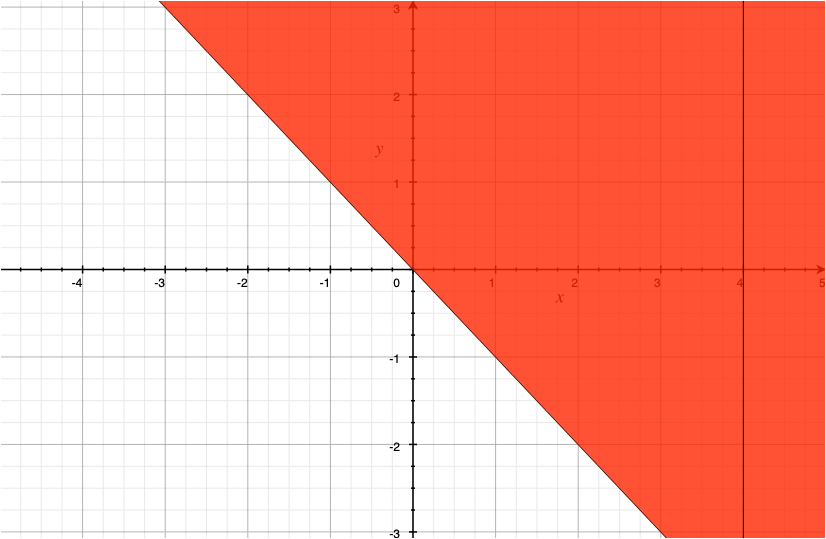
\includegraphics[width=0.5\textwidth]{Analisi2/figures/dominio_log(x+y)_x-4.jpg}
        \caption{Grafico di $D=\{(x,y)\in\mathbb R^2\;;\; x+y>0,\, x\neq 4\}$.}\label{fig:dominio_log(x+y)_x-4}
    \end{figure}
\end{example}

\begin{remark}[Non ufficiale]\footnote{Slide 8 PDF 11.}
    Per le funzioni di una o di più variabili il grafico è un sottoinsieme dello spazio in $n+1$ dimensioni. Quindi, per le funzioni in due variabili il grafico è l'insieme di terne $(x,y,z)$ tale per cui $z=f(x,y)$ con $(x,y)\in D$, ovvero: data $f\colon I\subseteq\mathbb R^2\rightarrow\mathbb R,\quad graf\;f =\{(x,y,z)\in\mathbb R^3\;;\;(x,y)\in D,\, z=f(x,y)\}\subseteq\mathbb R^3$. Per una funzione di una variabile $f\colon I\subseteq\mathbb R\rightarrow\mathbb R,\; graf\;f =\{(x,y)\in\mathbb R^2\;;\; y=f(x),\, \forall x\in I\}\subseteq\mathbb R^2$.
\end{remark}

\paragraph{N.B.:} \textbf{Sarà trattato solo il grafico di funzioni in due variabili perché oltre non $\boldsymbol n$ dimensioni è possibile rappresentarlo. Non è possibile rappresentare un grafico di una funzione in tre variabili perché sarebbe in 4 dimensioni, e così via.}

\paragraph{N.B.:} Per rappresentare il grafico di una funzione in 2 variabili, ovvero un sottoinsieme di $\mathbb R^3$, sono utilizzate le sezioni. Le sezioni tagliano il grafico con dei piano paralleli agli assi coordinati. Ad esempio: fissato $z=k$, il grafico è affettato ad altezza $k$ ed è intersecato con il piano $(x,y)$. Se $x=k$ il grafico è intersecato con il piano $(y,z)$. Se $y=k$, il grafico è intersecato con il piano $(x,z)$. Quindi, utilizzando le sezioni, il grafico non è più in $\mathbb R^3$ ma in $\mathbb R^2$.

\paragraph{N.B.:} Sarà trattato il grafico delle funzioni in due variabili utilizzando il concetto geometrico di sezione di insieme. Ovvero, è affettato il grafico in $\mathbb R^3$ in un piano $z$ costante diminuendo la dimensione del problema ad $\mathbb R^2$ tracciando delle sezioni del grafico in $\mathbb R^3$ nei piani
\begin{equation}\label{eq:piani}
    \begin{matrix}
        x=k\\
        y=k\\
        z=k
    \end{matrix}
\end{equation}

%slide 8 PDF 11
\begin{figure}
\centering
    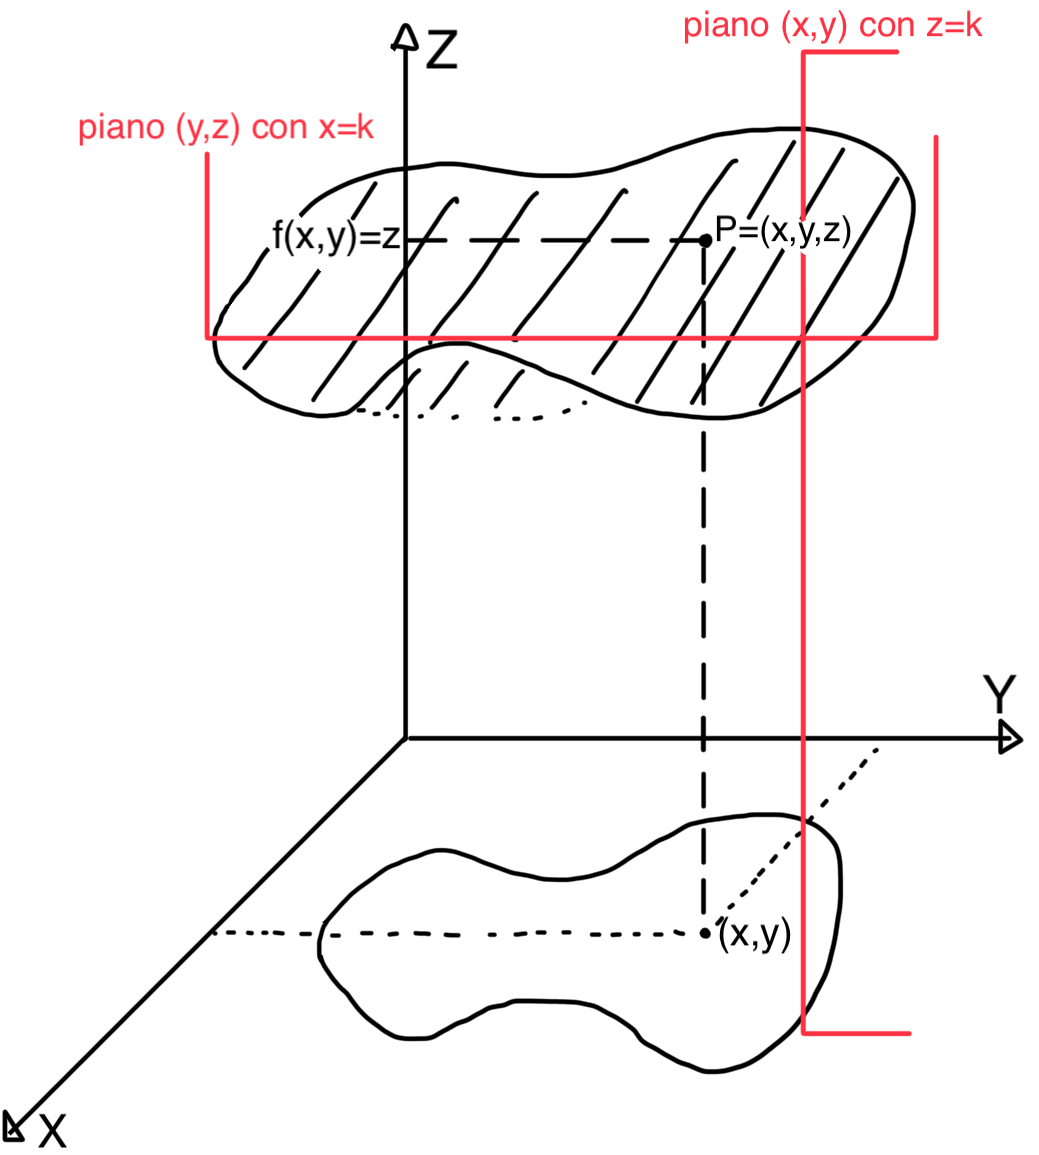
\includegraphics[width=0.75\textwidth]{Analisi2/figures/grafico_f_generica_R3.jpg}
    \caption{Grafico di $f$ funzione in due variabili.}\label{fig:grafico_f_generica_R3}
\end{figure}

Se intersecato il grafico con i piani (\ref{eq:piani}) (vedere Figura \ref{fig:grafico_f_generica_R3}) sono ottenute le sezioni trasversali del grafico. è utile utilizzare le sezioni per abbassare la dimensione del problema.

Considerato il grafico di $f$ definita in $\mathbb R^2$, questo è l'insieme di terne $(x,y,z)$. Considerate le sezioni è come se il grafico fosse tagliato con i piani $x=k,\, y=k,\, z=k$, dove $k\in\mathbb R$ è una costante. Ad esempio, con il seguente sistema è ottenuta l'intersezione del piano $y=k$ con il grafico di $f$ (sulle $y$)
\begin{equation*}
    \begin{cases}
        y=k\\
        z=f(x,y)
    \end{cases}\equiv
    \begin{cases}
        graf\,f\\
        y=k
    \end{cases}
\end{equation*}

\begin{example}\footnote{Slide 9 PDF 11.}\label{example:disegnare_tracce_x^2-y}
    Sia $f(x,y)=x^2-y$, dove $f\colon\mathbb R^2\rightarrow\mathbb R$. Disegnarne le tracce.\\
    $graf\,f=\{(x,y,z)\in\mathbb R^3,\, (x,y)\in\mathbb R^2,\, z=x^2-y\}$.\\
    Considerando la regione $x=k$ (ovvero l'intersezione del grafico con il piano $(y,z)$)
    \begin{equation}\label{eq:esempio_intersezione_piano_y_z}
        \begin{cases}
            graf\, f\\
            x=k
        \end{cases}\rightarrow
        \begin{cases}
            z=f(x,y)=f(k,y)\\
            x=k
        \end{cases}
    \end{equation}
    \footnotemark e dunque è ottenuto un insieme nel piano $(y,z)$
    \begin{equation}\label{eq:fascio_rette_nel_piano}
        \begin{cases}
            z=x^2-y\\
            x=k
        \end{cases}\longrightarrow z=-y+k^2\quad \forall k\in\mathbb R.
    \end{equation}
    Quindi $z$ è un fascio di rette parallele con coefficiente -1, vedere Figura \ref{fig:esempio_z=-y+k2}. \footnotemark\\
    Cambiando le regioni con $y=k$,
    \begin{equation}\label{eq:esempio_intersezione_piano_x_z}
        \begin{cases}
            graf\, f\\
            y=k
        \end{cases}\rightarrow
        \begin{cases}
            z=f(x,y)=f(x,k)\\
            y=k
        \end{cases}
    \end{equation}
    Tale regione (sezione) è un insieme nel piano $(x,z)$ che è dato dal grafico della funzione $z=f(x,k)$ nel piano $(x,z)$. (Ciò cosa significa? \footnotemark).\\
    (Quindi, se il grafico di $f$ è tagliato facendolo intersecare con il piano $(x,z)$ sono ottenute parabole, vedere Figura \ref{fig:esempio_z=x^2-k}, oppure se intersecato con il piano $(y,z)$ sono ottenute rette, vedere Figura \ref{fig:esempio_z=-y+k2}).\\
    Considerando la regione $z=k$,
    \begin{equation}\label{eq:esempio_intersezione_piano_x_y}
        \begin{cases}
            graf\, f\\
            z=k
        \end{cases}\rightarrow
        \begin{cases}
            z=f(x,y)=f(x,y)\\
            z=k
        \end{cases}
    \end{equation}
    il grafico è un oggetto è nel piano $(x,y)$ ed è formato dalle coppie $(x,y)\in D$ tali che $f(x,y)=k$, al variare di $k$ (Vedere Figura \ref{fig:esempio_z=k=x^2-y}).
\end{example}
\addtocounter{footnote}{-2}
\footnotetext{(\ref{eq:esempio_intersezione_piano_y_z}) rappresenta il grafico della funzione nel piano $(y,z)$, dove $z$ è in funzione di $y$ (ovvero $f$ è una funzione di una variabile). Osservando la Figura \ref{fig:grafico_f_generica_R3}, quando $y=k$, dove $k$ è una costante, significa che è tagliato il piano $(y,z)$ nel grafico di $f$ ed $f$ diventa in funzione di $y$. In modo analogo, se $x=k$, il piano del grafico è $(x,z)$. Inoltre, se $z=k$ allora il piano è $(x,y)$.}

\stepcounter{footnote}
\footnotetext{Nel piano $(x,y)$, quello disegnato in Figura \ref{fig:esempio_z=-y+k2}, è sezionato il grafico (in 3 dim.) della funzione con il piano $y=k$, trovando tutte le rette di pendenza $-1$ e parallele alla retta $z=-y$ (ovveo del tipo $z=-y+k^2$ in (\ref{eq:fascio_rette_nel_piano}).}

\stepcounter{footnote}
\footnotetext{(\ref{eq:esempio_intersezione_piano_x_z})$\equiv z=f(x,k)=x^2-k$, ovvero fasci di rette. Quindi, le sezioni del grafico di $f$ sono date da parabole, come descritto in Figura \ref{fig:esempio_z=x^2-k}. Il grafico di $f$ è in 3 dimensioni, ma se tagliato con $y=k$ è intersecato con il piano $(y,z)$.}

%slide 10 PDF 11
\begin{figure}
\centering
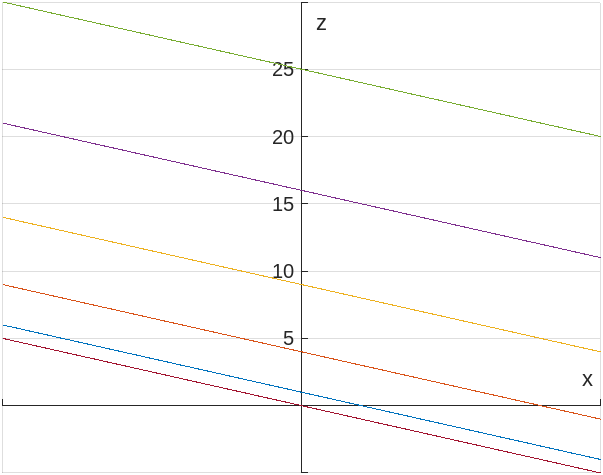
\includegraphics[width=0.5\textwidth]{Analisi2/figures/esempio_z=-y+k2.png}
    \caption{Grafico di $z=-y+k^2$, con $k\in[-5,5]\subset\mathbb N$ (nella realtà è $\forall k\in\mathbb R$).}\label{fig:esempio_z=-y+k2}
\end{figure}

\begin{figure}
\centering
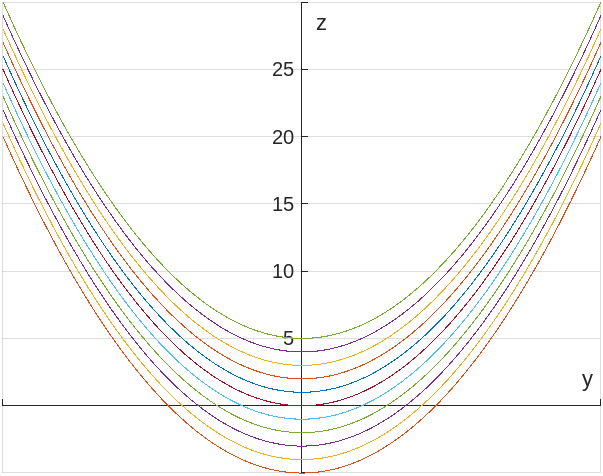
\includegraphics[width=0.5\textwidth]{Analisi2/figures/esempio_z=x^2-k.png}
    \caption{Grafico di $z=x^2-k$, con $k\in[-5,5]\subset\mathbb N$ (nella realtà è $\forall k\in\mathbb R$).}\label{fig:esempio_z=x^2-k}
\end{figure}

\begin{figure}
\centering
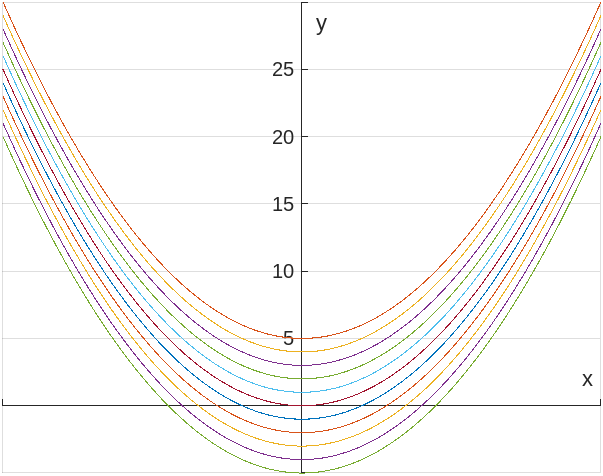
\includegraphics[width=0.5\textwidth]{Analisi2/figures/esempio_z=x^2-y.png}
    \caption{Grafico di $z=k=x^2-y$, con $k\in[-5,5]\subset\mathbb N$ (nella realtà è $\forall k\in\mathbb R$).}\label{fig:esempio_z=k=x^2-y}
\end{figure}

\paragraph{N.B.:} In Figura \ref{fig:esempio_z=k=x^2-y}, il paraboloide sezionato nel piano $(x,y)$ per $k\in\mathbb R$ avrà un oggetto nel dominio.

\begin{definition}[Insieme (o curve) di livello $k$]\footnote{Slide 12 PDF 11.}
    Data $f:D\subseteq\mathbb R^n\rightarrow\mathbb R$, l'insieme di livello $k$ è definito come
    \begin{equation}\label{eq:insime_livello_k_Rn}
        E_k=\{\uline x\in D\,|\, f(\uline x)=k,\, k\in\mathbb R\}\subset\mathbb R.
    \end{equation}
\end{definition}

\begin{remark}[Non ufficiale]
    Nel caso di funzioni di due variabili, l'insieme di livello $k$ è dato dagli elementi del dominio $(x,y)\in D$ tali che è risolto $f(x,y)=k$. Ciò si ha quando è considerata la regione $z=k$, quindi l'intersezione del grafico di $f$ con il piano $(x,y)$.
\end{remark}

\begin{remark}\footnote{Slide 8 PDF 14.}
    Se un insieme di livello $E_k$ ha livello $k$ non raggiungibile da $f$ allora $E_k=\emptyset$. Ad esempio, se $k<0$ e $f(x,y)=x^2+y^2$ allora $\nexists(x,y)\in\mathbb R^2$ tali che $f(x,y)=x^2+y^2=k$, quindi $E_k=\emptyset$.
\end{remark}

\paragraph{N.B.:} Gli insiemi (o curve) di livello sono chiamati così perché a volte rappresentano delle curve nel piano (esempio: carte topologiche).

\paragraph{N.B.:} Un insieme è detto di livello $k$ perché quando sono considerate le curve di livello sul piano $(x,y)$, per ottenere un grafico in $\mathbb R^3$ è sufficiente "tirare su" i punti attraverso la funzione. Questo perché il grafico di $f$ è dato da $z=f(x,y)$. In altre parole: preso un punto in $E_k$, è assegnata la quota $z$ e così è assegnato il punto nel grafico.

\begin{example}
    Sia l'Esempio \ref{example:disegnare_tracce_x^2-y}. Considerando $z=f(x,y)$ intersecato con $z=k$, l'insieme di livello $k$ è $E_k=\{(x,y)\in\mathbb R^2\,|\, x^2-y=k\}$.
\end{example}

\begin{exercise}\footnote{Slide 1 PDF 12.}
    Determinare l'insieme di definizione $E\subseteq\mathbb R^2$ della funzione
    \begin{equation*}
        f(x,y)=\frac{\log(x^3-y)}{\sqrt{1-xy}}.
    \end{equation*}
    \begin{equation*}
        \begin{matrix}
            E &=& \{(x,y)\in\mathbb R^2\,|\, x^3-y>0,\,\sqrt{1-xy}\neq 0,\, 1-xy> 0\} &=& \{(x,y)\in\mathbb R^2\,|\, y<x^3,\, 1-xy>0\}\\
            &=& \{(x,y)\in\mathbb R^2\,|\, y<x^3,\, xy-1<0\} &=&\{(x,y)\in\mathbb R^2\,|\, y<x^3,\, xy<1\}.
        \end{matrix}
    \end{equation*}
    $E$ è un illimitato e aperto.
    Vedere Figura \ref{fig:esempio_dominio_analisi2_1}.
    \begin{figure}
    \centering
    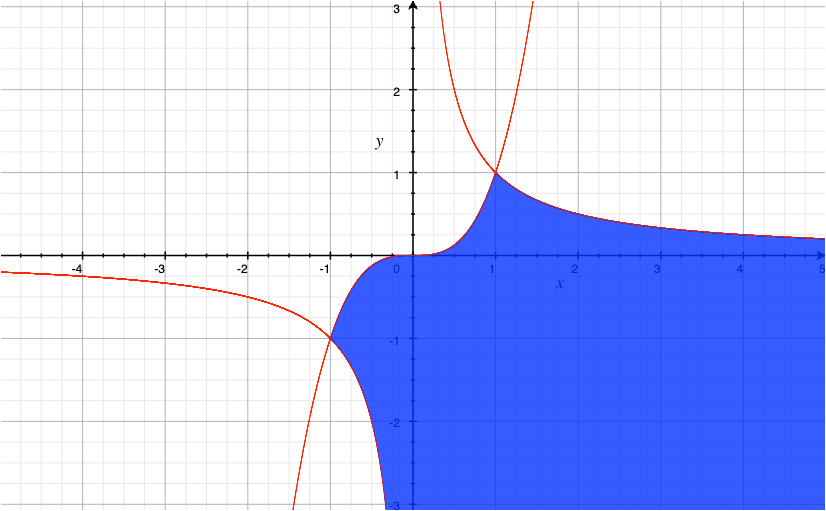
\includegraphics[width=0.65\textwidth]{Analisi2/figures/esempio_dominio_analisi2_1.jpg}
        \caption{Grafico di $E=\{(x,y)\in\mathbb R^2\,|\, x^3-y>0,\,\sqrt{1-xy}\neq 0,\, 1-xy\geq 0\}=\{(x,y)\in\mathbb R^2\,|\, y<x^3,\, 1-xy>0\}$.}\label{fig:esempio_dominio_analisi2_1}
    \end{figure}
\end{exercise}

\begin{example}\footnote{Slide 8 PDF 12.}
    I punti $(x,y)\in\mathbb R^2$ che sono nell'insieme di livello $k=1$ della funzione $f(x,y)=x^2+y^2$ sono i punti che verificano $x^2+y^2=1$, ovvero:
    \begin{equation*}
        E_1=\{(x,y)\in\mathbb R^2\,|\, f(x,y)=1\}=B(\uline 0, 1).
    \end{equation*}
    Vedere Figura \ref{fig:E_1}.
    \begin{equation*}
        E_k=\{(x,y)\in\mathbb R^2\,|\, x^2+y^2=k\}.
    \end{equation*}
    \begin{enumerate}
        \item Se $k<0$ allora $E_k=\{(x,y)\in\mathbb R^2\,|\, x^2+y^2<k\}=\emptyset$,
        \item Se $k=0$ allora $E_0=\{(x,y)\in\mathbb R^2\,|\, x^2+y^2=0\}=\{(0,0)\}$,
        \item Se $k>0$ allora $E_k=\{(x,y)\in\mathbb R^2\,|\, x^2+y^2>k\}=B(\uline 0,\sqrt{k})$.
    \end{enumerate}
    Vedere Figura \ref{fig:E_k_2D} e Figura \ref{fig:E_k_3D}. La Figura \ref{fig:E_k_3D_1} fa vedere come le sezione "tirate su" disegnino il grafico di $f(x,y)=x^2+y^2$.
    
    \begin{figure}
    \centering
    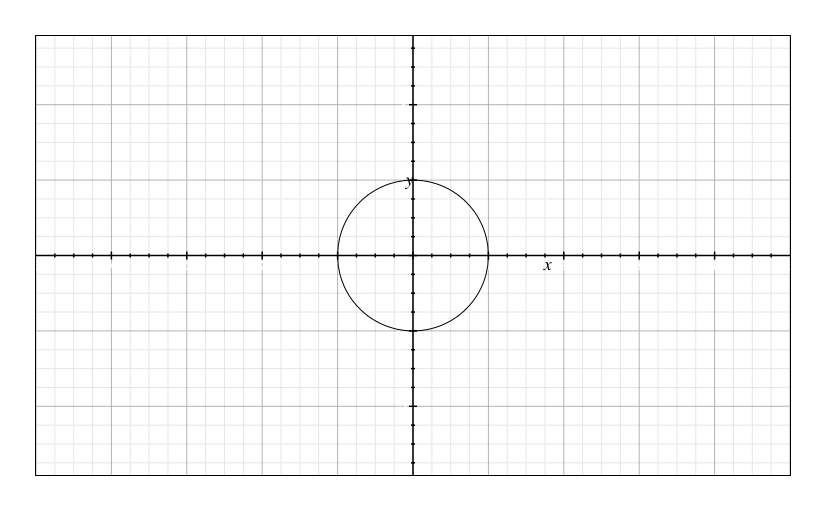
\includegraphics[width=0.65\textwidth]{Analisi2/figures/E_1.jpg}
        \caption{Grafico di $E_1=\{(x,y)\in\mathbb R^2\,|\, f(x,y)=1\}=B(\uline 0, 1)$.}\label{fig:E_1}
    \end{figure}
    
    \begin{figure}
    \centering
    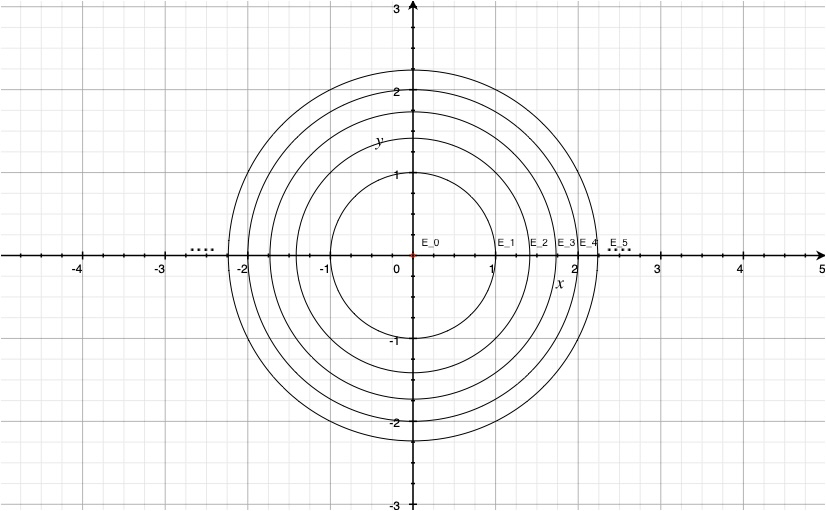
\includegraphics[width=0.65\textwidth]{Analisi2/figures/E_k_2D.jpg}
        \caption{Grafico di $E_k=\{(x,y)\in\mathbb R^2\,|\, x^2+y^2=k\}=B(\uline 0, \sqrt{k})$.}\label{fig:E_k_2D}
    \end{figure}
    
    \begin{figure}
    \centering
    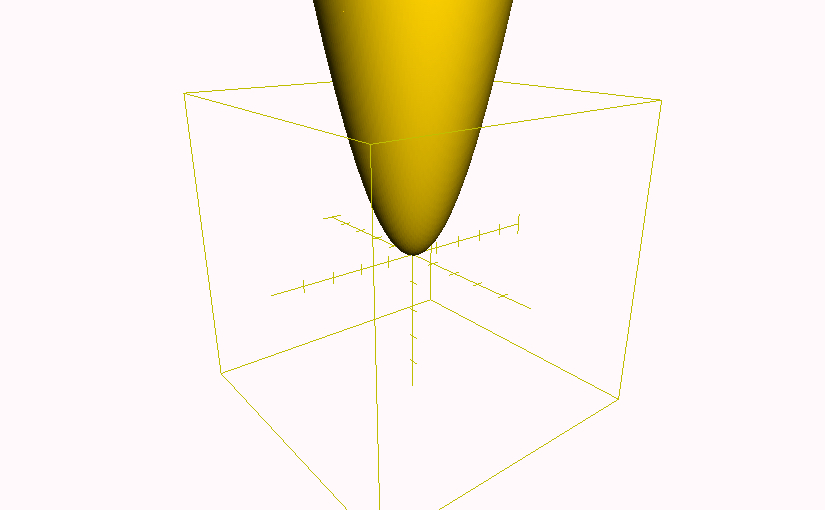
\includegraphics[width=0.65\textwidth]{Analisi2/figures/E_k_3D.jpg}
        \caption{Grafico di $z=f(x,y)=x^2+y^2$.}\label{fig:E_k_3D}
    \end{figure}
    
    \begin{figure}
    \centering
    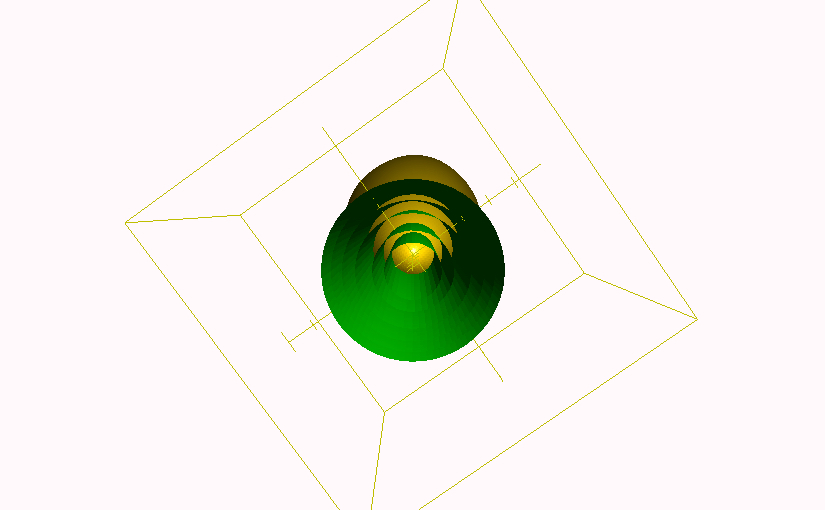
\includegraphics[width=0.65\textwidth]{Analisi2/figures/E_k_3D_1.jpg}
        \caption{Grafico di $z=f(x,y)=x^2+y^2$ intersecato con $E_k$.}\label{fig:E_k_3D_1}
    \end{figure}
\end{example}

\begin{example}\footnote{Slide 13-15 PDF 12.}
    Disegnare l'insieme di livello $E_k$ delle seguenti funzioni $f\colon E\subseteq\mathbb R^2\rightarrow\mathbb R$:
    \begin{enumerate}
        \item (per casa) $z=x+2y$.
        \item $z=x^2+9y^2$.
        \begin{equation*}
            E_k=\{(x,y)\in\mathbb R^2\,|\,x^2+9y^2=k\}.
        \end{equation*}
        \begin{itemize}
            \item $k<0\Longrightarrow E_k=\emptyset$,
            \item $k=0 \Longrightarrow E_k=\{(0,0)\}$,
            \item $k>0$ \footnote{Quando $k>0$ allora $x^2+9y^2=k$ rappresenta un'ellissi negli assi $(x,y)$. Un ellisse di semiassi $a$ e $b$ ha la forma in Figura \ref{fig:esempio_ellisse} ed è espresso come (\ref{eq:ellisse_assi_a,b}). È necessario portare l'ellisse in una forma conosciuta, ovvero in forma (\ref{eq:ellisse_assi_x,y}) (dai semiassi $(a,b)$ a $(x,y)$). La trasformazione da asse $(a,b)$ in asse $(x,y)$ è fatta  dividendo per $(\sqrt{x})^2=k$, il quale rappresenta $a^2$, e $\left(\sqrt{\frac{k}{2}}\right)^2$, il quale rappresenta $b^2$.} 
            \begin{equation}\label{eq:ellisse_assi_a,b}
                \frac{x^2}{a^2}+\frac{y^2}{b^2}=1
            \end{equation}
            allora
            \begin{equation}\label{eq:ellisse_assi_x,y}
                \frac{x^2}{\left(\sqrt{k}\right)^2}+\frac{y^2}{\left(\frac{\sqrt{k}}{3}\right)^2}=1.
            \end{equation}
            \begin{figure}
            \centering
            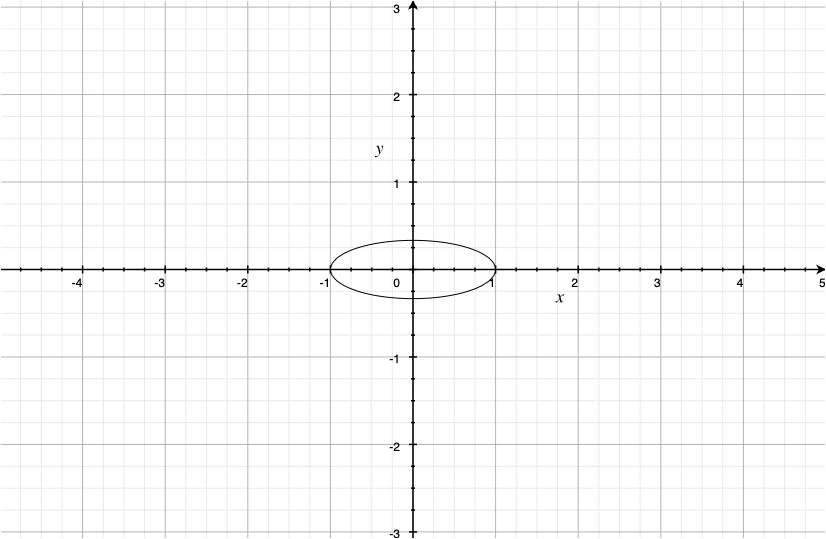
\includegraphics[width=0.5\textwidth]{Analisi2/figures/esempio_ellisse.jpg}
                \caption{Grafico di $f(x,y)=x^2+9y^2$.}\label{fig:esempio_ellisse}
            \end{figure}
        \end{itemize}
        \item $z=\frac{2x}{x^2+y^2}.\, f:E=\mathbb R^2\backslash\{(0,0)\}\rightarrow\mathbb R.$
        \begin{equation*}
            E_k=\left\{(x,y)\in E\,|\, \frac{2x}{x^2+y^2}=k\right\}.
        \end{equation*}
        \begin{itemize}
            \item Se $k=0\Rightarrow E_0=\left\{(x,y)\in E\,|\, \frac{2x}{x^2+y^2}=0\right\}=\{x=0, \text{ con } y\neq 0\},$
            \item Se $k\neq 0\Rightarrow E_k=\left\{(x,y)\in E\,|\, \frac{2x}{x^2+y^2}=k\right\}\Rightarrow\frac{2x}{x^2+y^2}=k\Rightarrow 2x=kx^2+ky^2\Rightarrow kx^2+ky^2-2x=0\Rightarrow$ con $\left(x-\frac{1}{k}\right)^2+y^2=\frac{1}{k^2 },\, \underbrace{x^2+y^2-\frac{2}{k}x=0}_{B\left(\left(\frac{1}{k},\, 0\right),\frac{1}{k}\right)}.$
        \end{itemize}
        \item $z=\frac{y}{x^2}.\, E=\left\{(x,y)\in\mathbb R^2\,|\, x\neq 0\right\}$ (unione di due semipiani).
        \begin{equation*}
            E_k=\left\{(x,y)\in E\,|\, \frac{y}{x^2}=k\right\}.
        \end{equation*}
        \begin{itemize}
            \item Se $k=0\Rightarrow E_0=\{y=0,\text{ con } x\neq 0\}$ (asse $x$ privata di $(0,0)$),
            \item $k>0 \Rightarrow E_k=\left\{(x,y)\in E\,|\, \frac{y}{x^2}=k\right\}=\{(x,y)\in E\,|\, y\overset{\footnotemark}{=}kx^2\}$ (parabola con vertice $V=(0,0)$ escluso e concavità verso l'alto),
            \item $k<0\Rightarrow E_k=\{(x,y)\in E\,|\, y=kx^2\}$ (parabola con vertice $V=(0,0)$ escluso e concavità verso il basso).
        \end{itemize}
        \begin{figure}
        \centering
        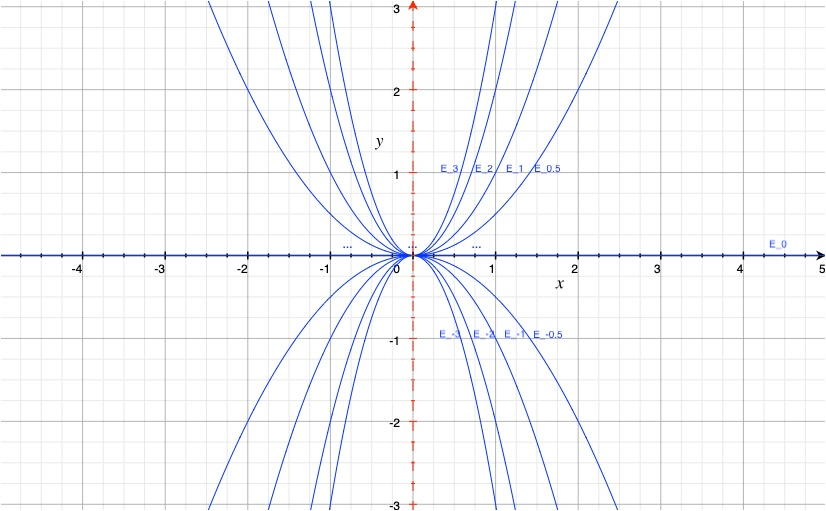
\includegraphics[width=0.65\textwidth]{Analisi2/figures/esempio_E_k.jpg}
            \caption{Grafico di $E_k=\left\{(x,y)\in E\,|\, \frac{y}{x^2}=k\right\}$ (asse $y$ escluso).}\label{fig:esempio_E_k}
        \end{figure}
    \end{enumerate}
\end{example}

\paragraph{Insiemi del piano determinati da equazioni o disequazioni (in due variabili)} La questione è legata alle proprietà di continuità delle funzioni in due variabili e alle funzioni in una variabile.\\
Sia $f\colon I=[a,b]\subseteq\mathbb R\rightarrow\mathbb R$ continua, dove grafico $graf\, f=\{(x,y)\in\mathbb R^2\,|\, y=f(x),\; x\in I\}\subseteq\mathbb R^2$ descrive una curva \footnotemark continua come in Figura \ref{fig:grafico_f_R2}. Sono date le definizioni di sotto/sopra/semigrafico (e sono valide anche con $<$ al posto di $\leq$).
\footnotetext{In matematica le curve sono operazioni definite da un intervallo ad un insieme, a seconda che le curve siano piane o nello spazio $\mathbb R^n$. Nel caso di Figura \ref{fig:grafico_f_R2} la curva è piana, dove è possibile pensarla come arco di curva continua.}

\begin{figure}
    \centering
    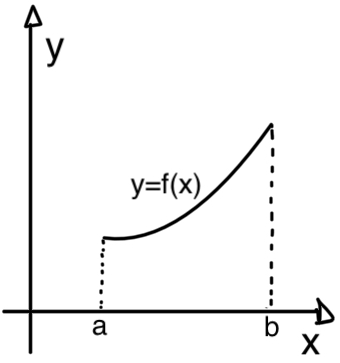
\includegraphics[width=0.5\textwidth]{Analisi2/figures/grafico_f_R2}
        \caption{Grafico di $y=f(x)$.}\label{fig:grafico_f_R2}
\end{figure}

\begin{definition}[Sottografico]\footnote{Slide 2 PDF 12.}
    Il sottografico di $f$ è definito come
    \begin{equation*}
        \{(x,y)\in\mathbb R^2\,|\, y\leq f(x),\, x\in I\}\subseteq\mathbb R^2.
    \end{equation*}
    Vedere Figura \ref{fig:sottografico_f_R2}.
\end{definition}
\begin{definition}[Sopragrafico]\footnote{Slide 3 PDF 12.}
    Il sopragrafico di $f$ è definito come
    \begin{equation*}
        \{(x,y)\in\mathbb R^2\,|\, y\geq f(x),\, x\in I\}\subseteq\mathbb R^2.
    \end{equation*}
    Vedere Figura \ref{fig:sopragrafico_f_R2}.
\end{definition}

\begin{definition}[Semipiano]\footnote{Slide 3 PDF 12.}
    Un semipiano è determinato da una equazione di grado 1.
\end{definition}

\begin{figure}
    \centering
    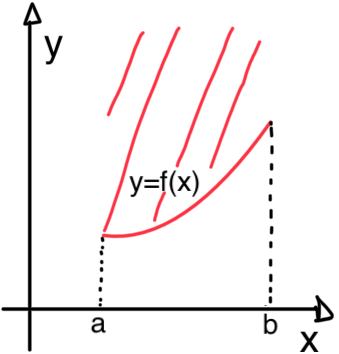
\includegraphics[width=0.5\textwidth]{Analisi2/figures/sopragrafico_f_R2.jpg}
        \caption{Sopragrafico di $y=f(x)$.}\label{fig:sopragrafico_f_R2}
\end{figure}

\begin{figure}
    \centering
    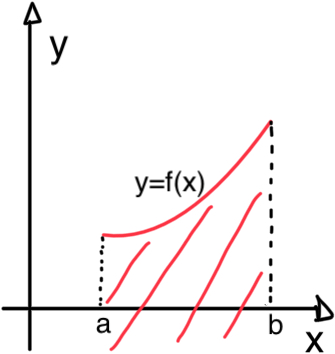
\includegraphics[width=0.5\textwidth]{Analisi2/figures/sottografico_f_R2.jpg}
        \caption{Sottografico di $y=f(x)$.}\label{fig:sottografico_f_R2}
\end{figure}

\begin{example}\footnote{Slide 4 PDF 12.}
    Sia $2x-3y+1\geq 0$. $2x-3y+1=0$ è una retta ed un semipiano, in quanto $3y=2x+1$, ovvero $y=\frac{2x+1}{3}$. Quindi, la disequazione è il sottografico della retta (per $-3y$). Vedere Figura \ref{fig:esempio_sottografico}.
    \begin{figure}
    \centering
    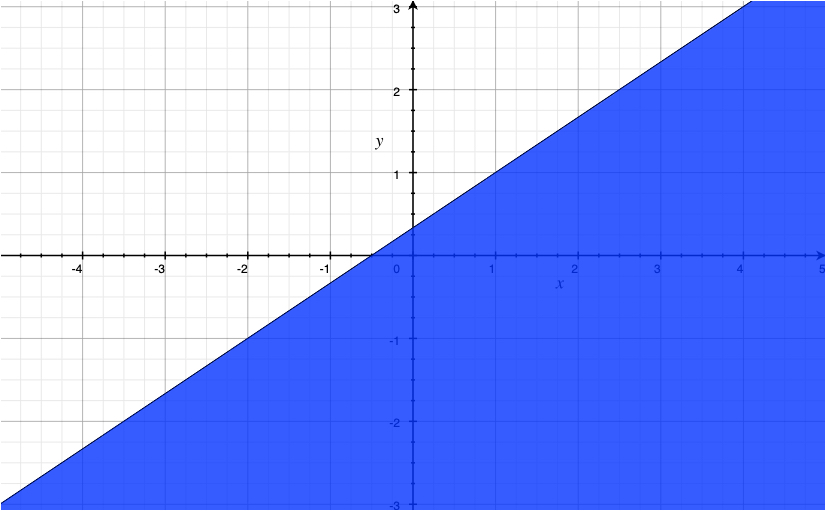
\includegraphics[width=0.5\textwidth]{Analisi2/figures/esempio_sottografico.jpg}
        \caption{Sottografico di $2x-3y+1=0$.}\label{fig:esempio_sottografico}
    \end{figure}
\end{example}

\begin{example}\footnote{Slide 4 PDF 12.}
    Trovare i punti del piano per i quali  è verificata la disequazione
    \begin{equation}\label{eq:esempio_disequazione}
        x^2-y^2\geq 1.
    \end{equation}
    Definita $f(x,y)=x^2-y^2-1$, una funzione continua $\forall(x,y)\in\mathbb R^2$, allora la disequazione (\ref{eq:esempio_disequazione}) è equivalente a $f(x,y)\geq 0$.
    
    Consideriamo cosa accade quando $f(x,y)=0$, ovvero consideriamo l'insieme di punti sottoinsieme di $\mathbb R^2$ tali che $x^2-y^2-1=0$ (ovvero, l'iperbole traslata passante in $\pm 1$ sia uguale a 0).
    Vedere Figura \ref{fig:grafico_x^2-y^2-1}. $f(x,y)$ divide il piano in 3 zone illimitate, ovvero 3 insiemi aperti e connessi: $A_1,\, A_2,\, A_3$ nei quali $f(x,y)\neq 0$ ed è continua. In ciascuna delle 3 regioni il segno non cambia \footnote{Il segno non cambia perché in ognuna di esse $f\neq 0$ ed è continua. Ciò significa che per mostrare quanto vale il segno di $f$ in ogni zona è sufficiente calcolarla in un punto comodo. I punti comodi interessanti nell'esempio sono l'origine perché in $A_2$, $(2,0)$ perché in $A_3$ e $(-2,0)$ perché in $A_1$.}
    \begin{itemize}
        \item $f(0,0)=-1<0,\quad f(x,y)<0\;\forall (x,y)\in A_2$,
        \item $f(2,0)=4-1=3>0\quad f(x,y)>0\; \forall (x,y)\in A_3$,
        \item $f(-2,0)=4-1=3>0\quad f(x,y)>0\; \forall (x,y)\in A_1$.
    \end{itemize}
    
    Nelle tre regioni $f$ ha segno costante ed è continua, quindi dove è diversa da 0 $f$ ha l'insieme immagine formata da un aperto (in questo caso l'unione di aperti) connesso.

    Essendo il segno 0 nelle due parabole, questo cambia passando fra $A_1,\, A_2$ e $A_3$. Ovvero: in $A_1$ e $A_3$ il segno è positivo ed in $A_2$ il segno è negativo, quindi \uline{vale il Teorema \ref{th:esistenza_degli_zeri} degli zeri in più dimensioni}.
    
    \begin{figure}
    \centering
    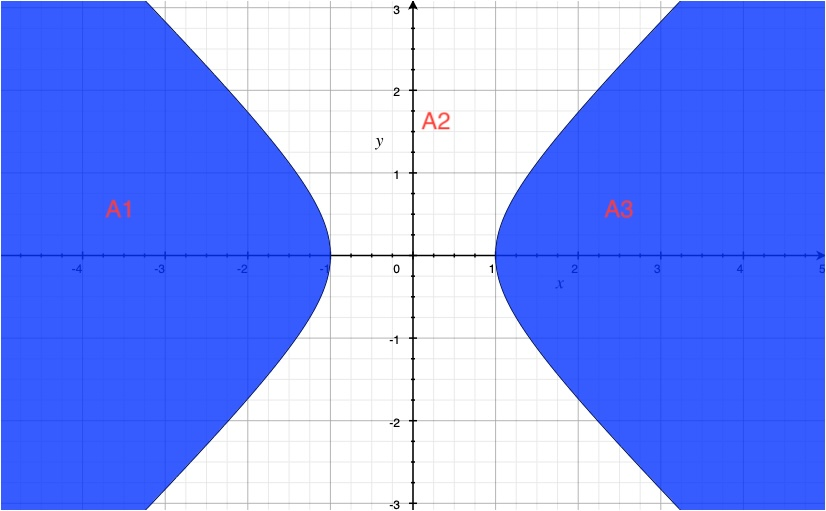
\includegraphics[width=0.65\textwidth]{Analisi2/figures/grafico_x^2-y^2-1.jpg}
        \caption{Sottografico di $2x-3y+1=0$.}\label{fig:grafico_x^2-y^2-1}
    \end{figure}
\end{example}

Dall'esempio è possibile affermare che se $f(x,y)$ è continua in $\mathbb R^2$, allora quando $f(x,y)\neq 0$ (è importante che sia diverso da 0) definisce un aperto del piano dato dall'unione di un certo numero di aperti connessi sul quale $f$ è definita ed è diversa da 0. Nell'esempio $f(x,y)\neq 0$ su $A_1\cup A_2\cup A_3$.

Supponendo gli aperti siano in un numero finito, ovvero: $A_1,\, A_2,\, \hdots, A_n$. È utile studiare il segno di $f(x,y)$ in ogni $A_i$ (quindi dove $f(x,y)\neq 0$).

\paragraph{Osservazioni sullo studio di $\boldsymbol{A_1}$ dell'esempio precedente:} In $A_1$ $f(x,y)\neq 0$, dunque $f(x,y)>0$ oppure $f(x,y)<0$. Dal momento che $f$ è continua ed il suo segno non può cambiare (per ipotesi) e $A_1$ è aperto e connesso, il segno di $f$ non cambia in $A_1$. Se così non fosse, esisterebbero in $A_1$ due punti distinti in cui $f(x,y)$ ha segno opposto e quindi, per il Teorema \ref{th:esistenza_degli_zeri} degli zeri, esisterebbe un punto $(x,y)\in A_1$ tale che $f(x,y)=0$. Quindi, $f(x,y)$ ha segno costante in $A_1$. Pertanto, per valutare il segno di $f$ in $A_1$ è sufficiente valutare il segno di $f$ in un punto qualsiasi di $A_1$ (come fatto nell'elenco dell'esempio).\\
Lo stesso ragionamento si ripete su ogni regione (piano) $A_i$ (quindi in ogni regione $A_i$ la funzione ha lo stesso segno).

\begin{example}\footnote{Slide 10-12 PDF 12.}
    Trovare il campo di esistenza $E$ delle seguenti funzioni
    \begin{equation*}
        \begin{aligned}
            f\colon E\subseteq\mathbb R^2 &\rightarrow \mathbb R.\\
            (x,y)&\mapsto z=f(x,y)
        \end{aligned}
    \end{equation*}
    \begin{enumerate}
        \item Sia $z=\sqrt{1-x^2-y^2}$, allora
        \begin{equation*}
            E=\{(x,y)\in\mathbb R^2\,|\, 1-x^2-y^2\geq 0\}=\{(x,y)\in\mathbb R^2\,|\, x^2+y^2\leq 1\}.
        \end{equation*}
        $E$ è chiuso e (quindi) limitato. Vedere Figura \ref{fig:dominio_rad_1-x^2-y^2}.
        \item Sia $z=\sqrt{1-x^2}+\sqrt{1-y^2}$, allora
        \begin{equation*}
            \begin{matrix}
                E&=&\{(x,y)\in\mathbb R^2\,|\, 1-x^2\geq 0,\, 1-y^2\geq 0\}&=&\\
                &=&\{(x,y)\in\mathbb R^2\,|\, x^2\leq 1,\, y^2\leq 1\}&=&\{(x,y)\in\mathbb R^2\,|\, -1\leq x\leq 1,\, -1\leq y\leq 1\}.
            \end{matrix}
        \end{equation*}
        $E$ è chiuso. Vedere Figura \ref{fig:dominio_rad_1-x^2+rad_1-y^2}.
        \item Sia $z=\frac{1}{\sqrt{y-\sqrt{x}}}$ funzione razionale, allora
        \begin{equation*}
            E=\{(x,y)\in\mathbb R^2\,|\, y-\sqrt{x}>0,\, x\geq 0\}=\{(x,y)\in\mathbb R^2\,|\, y>\sqrt{x},\, x\geq 0\}.
        \end{equation*}
        $E$ è un sopragrafico. Inoltre, non è aperto, non è chiuso, è illimitato. Vedere Figura \ref{fig:domino_frac_1_rad_y-radx}.
    \end{enumerate}
    \begin{figure}
    \centering
    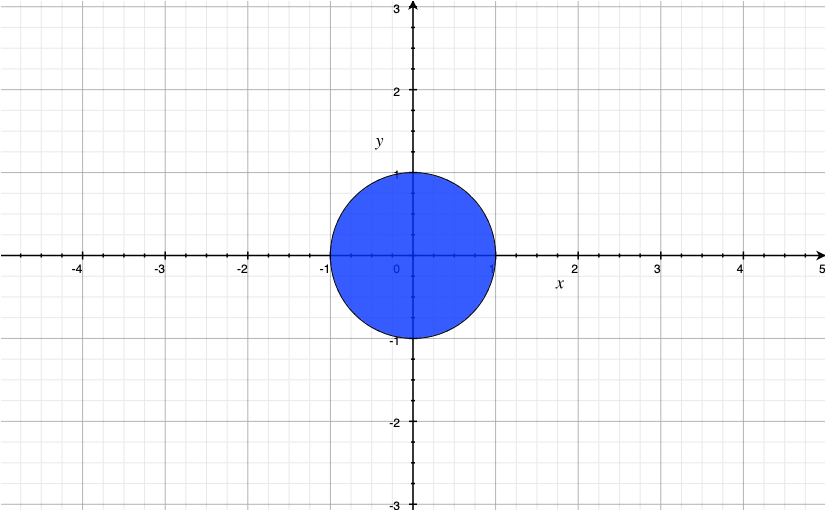
\includegraphics[width=0.65\textwidth]{Analisi2/figures/dominio_rad_1-x^2-y^2.jpg}
        \caption{Dominio $E=\{(x,y)\in\mathbb R^2\,|\, x^2+y^2\leq 1\}$ di $z=\sqrt{1-x^2-y^2}$.}\label{fig:dominio_rad_1-x^2-y^2}
    \end{figure}
    
    \begin{figure}
    \centering
    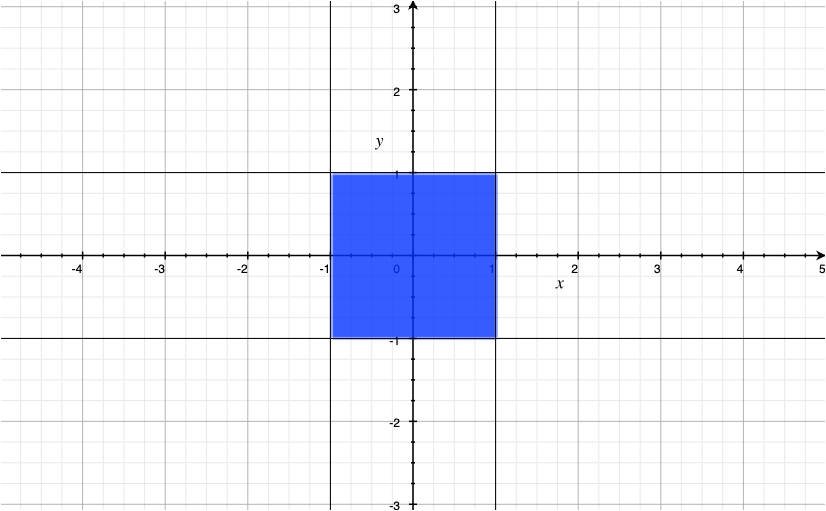
\includegraphics[width=0.65\textwidth]{Analisi2/figures/dominio_rad_1-x^2+rad_1-y^2.jpg}
        \caption{Dominio $E=\{(x,y)\in\mathbb R^2\,|\, 1-x^2\geq 0,\, 1-y^2\geq 0\}$ di $z=\sqrt{1-x^2}+\sqrt{1-y^2}$.}\label{fig:dominio_rad_1-x^2+rad_1-y^2}
    \end{figure}

    \begin{figure}
    \centering
    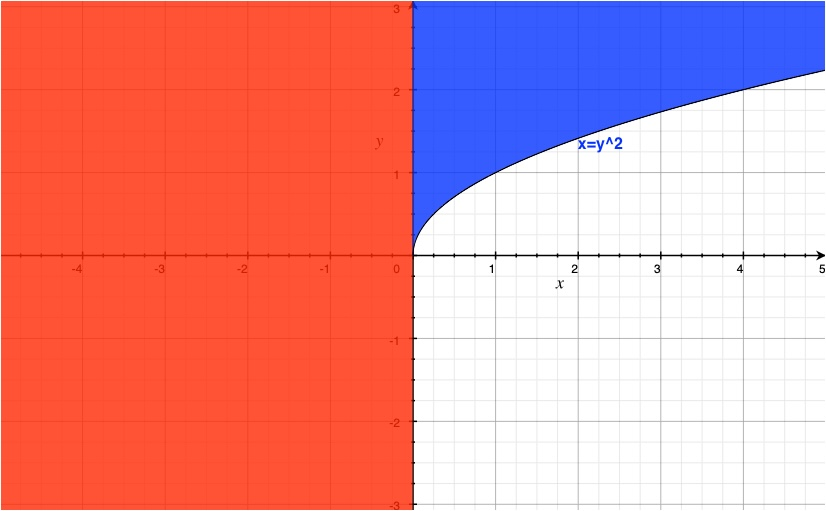
\includegraphics[width=0.65\textwidth]{Analisi2/figures/domino_frac_1_rad_y-radx.jpg}
        \caption{Dominio (in blu) $E=\{(x,y)\in\mathbb R^2\,|\, y>\sqrt{x},\, x\geq 0\}$ di $z=\frac{1}{\sqrt{y-\sqrt{x}}}$.}\label{fig:domino_frac_1_rad_y-radx}
    \end{figure}
\end{example}

INSERIRE TUTTO IL PDF 13

\subsubsection{Esempi sulla continuità}

\begin{example}\footnote{Slide 2 PDF 13.}
	\paragraph{Testo:} Stabilire se la
	\begin{equation*}
		f(x,y)=
		\begin{cases}
			\frac{x}{\log(x^2+y^2)}&\text{ per } (x,y)\neq(0,0)\\
			0 &\text{ altrimenti}
		\end{cases}
	\end{equation*}
	funzione è continua sul suo campo di esistenza.
	\paragraph{Svolgimento:} $f:\mathbb{R}^2\rightarrow\mathbb{R}$ e affinché risulti continua deve esistere il limite della funzione, per $(x,y)\rightarrow(0,0)$ e deve valere 0, ovvero
	\begin{equation*}
		\lim_{(x,y)\rightarrow(0,0)}f(x,y)=0.
	\end{equation*}
	Valutiamo dunque
	\begin{equation*}
		\left|\frac{x}{\log(x^2+y^2)}\right|\overset{\footnotemark}{=} \left|\frac{\rho \cos\theta}{\log(\rho^2)}\right| = \frac{\rho|\cos\theta|}{\underbrace{2|\log\rho|}_{\footnotemark}}\overset{\footnotemark}{\leq} \frac{\rho}{2|\log\rho|}\underset{\rho\rightarrow0^+}{\longrightarrow}0 .
	\end{equation*}
	\addtocounter{footnote}{-2}
	\footnotetext{Passaggio in cordinate polari. Inoltre, per la relazione fondamentale dell'aritmetica $\rho^2(\cos^2\theta+\sin^2\theta) = \rho^2\cdot 1$.}
	
	\stepcounter{footnote}
	\footnotetext{Proprietà dei logaritmi.}
	
	\stepcounter{footnote}
	\footnotetext{Le funzioni trigonometriche sono comprese fra $-1$ e $1$, quindi è possibile maggiorare.}
	
	\paragraph{Nota:} È stato utilizzato il Teorema del confronto \ref{th:dei_carabinieri_2} (detto dei carabinieri) sul valore assoluto di $f(x,y)$ trasformato in coordinate polari e maggiorato da una funzione rafiale maggiore uguale a 0. Pertanto, vale quanto segue. (Non è stato considerato il caso $\rho=0$, solo quello in cui $\rho\rightarrow 0^+$.) $\qed$
	
	\noindent Dunque,
	\begin{equation*}
		\lim_{(x,y)\rightarrow(0,0)} f(x,y) = 0 = f(0,0),
	\end{equation*}
	quindi $f$ è continua in tutto $\mathbb{R}^2$.
	
\end{example}

\paragraph{Nota:} Come in Analisi 1, prolungare la continuità signidica che nel punto incriminato $f$ è posto uguale al valore al quale tende la funzione quando $(x, y)$ tendono al punto incriminato.

\begin{example}\footnote{Slide 3 PDF 13}
	\paragraph{Testo:} Stabilire se la funzione
	\begin{equation*}
		f(x,y) \overset{\footnotemark}{=} \frac{\sin(\sqrt{x^2+y^2})}{\sqrt{x^2+y^2}}\quad \forall(x,y)\in\mathbb{R}^2\backslash\{(0,0)\}
	\end{equation*}
	\footnotetext{Il quoziente sono funzioni continue in $\mathbb{R}^2$, quindi è continuo in $\mathbb{R}^2\backslash\{(0,0)\}$.}
	
	\noindent è prolungabile con continuità in $(0,0)$ e stabilire quale valore deve assumere il prolungamento di $f$ in $(0,0)$.
	\paragraph{Cosa è necessario far vedere?} È necessario definire cosa accade in $(0,0)$ e per dimostrare che il prolungamento sia continui che il limite di $f(x,y)$, per $(x,y)\rightarrow(0,0)$ sia il valore della funzione in tale punto. È necessario ricordare che prolungare la continuità significa che l'immagine di $f$ in $(x_0,y_0)$ deve essere uguale al limite di $f$ per $(x,y)\rightarrow(x_0,y_0)$.
	\paragraph{Svolgimento:} È possibile osservare che $\forall (x,y)\in\mathbb R^2\backslash\{(0,0)\}$, $f$ è una funzione radiale (ovvero dipende solo da $\rho$), cioè
	\begin{equation*}
		f(x,y)=f(\rho)=\frac{\sin\rho}{\rho},
	\end{equation*}
	dove $\rho = d(\rho , \underline{0})$, con $\rho=(x,y)$.\\
	Quindi,
	\begin{equation*}
		\lim_{\rho\rightarrow0^+} f(\rho)=\lim_{\rho\rightarrow 0^+} \frac{\sin\rho}{\rho}=1.
	\end{equation*}
	\paragraph{Nota:} Quindi, se la funzione prolungata in $(0,0)$ vale 1, come il limite, allora la funzione è continua nel suo dominio e nel prolungamento (che non fa parte del dominio e vale 1).$\qed$\\
	Dunque 
	\begin{equation*}
		\tilde f(x,y)=
		\begin{cases}
			\frac{\sin(\sqrt{x^2+y^2})}{\sqrt{x^2+y^2}} &\text{ se } (x,y)\neq(0,0)\\
			1 & \text{ se } (x,y)=(0,0)
		\end{cases}
	\end{equation*}
	ovvero $\tilde f$ è continua su tutto il piano.
\end{example}

\begin{example}\footnote{Slide 5 PDF 13.}
	\paragraph{Testo:} Valutare il limite
	\begin{equation*}
		\lim_{(x,y)\rightarrow(0,0)} \frac{xy(2y^2 + 2 x^3)}{x^4+y^2}.
	\end{equation*}
	\paragraph{Svolgimento:} È calcolato lungo la retta $y=mx$ (dove se $y=0$ è necessario escludere $(0,0)$):
	\begin{equation*}
		\lim_{\underset{y=mx}{(x,y)\rightarrow (0,0)}} f(x,y)=\lim_{x\rightarrow 0}f(x,mx)=\lim_{x\rightarrow 0} \frac{x\,m\,x\,(2m^2x^2+x^3)}{x^4+m^2x^2}=\lim_{x\rightarrow 0}\frac{\cancel{x^2}\,m\, [x^2(2m^2-x)]}{\cancel{x^2}(x^2+m^2)} = \lim_{x\rightarrow 0}\frac{mx^2(2m^2-x)}{x^2+m^2}=0.
	\end{equation*}
	Quindi, il limite, se esiste, è 0. È necessario mostrare che è 0. Passando in coordinate polari
	\begin{equation*}
		\begin{cases}
			x=\rho\cos\theta\\
			y=\rho\sin\theta
		\end{cases}
	\end{equation*}
	è ottenuto
	\begin{equation*}
		\begin{matrix}
			\left|\frac{\rho^2\cos\theta \sin\theta (2\rho^2\sin^2(\theta)+\rho^3\cos^3(\theta))}{\rho^4\cos^4\theta + \rho^2 \sin^2\theta}\right| &=& \left|\frac{\cancel{\rho^2}cos\theta \sin\theta (2\rho^2\sin^2(\theta)+\rho^3\cos^3(\theta))}{\cancel{\rho^2}(\rho^2\cos^4\theta + \sin\theta^2\theta)}\right|&=& \left|\frac{2\rho^2\cos\theta\sin^3\theta + \rho^3 \cos^4\theta\sin\theta}{\rho^2 \cos^4\theta + \sin^2\theta}\right|\\\\
			&=& \left|\frac{2\rho^2\cos\theta\sin^3\theta}{\rho^2 \cos^4\theta + \sin^2\theta} + \frac{\rho^3 \cos^4\theta\sin\theta}{\rho^2 \cos^4\theta + \sin^2\theta}\right| &\overset{|x+y|\leq|x|+|y|}{\underset{\text{disug. triang.}}{\leq}}& \left|\frac{2\rho^2\cos\theta\sin^3\theta}{\rho^2 \cos^4\theta + \sin^2\theta}\right| + \left| \frac{\rho^3 \cos^4\theta\sin\theta}{\rho^2 \cos^4\theta + \sin^2\theta}\right|\\\\
			&&(\text{portate fuori cose $\geq0$})&=& \frac{2\rho^2|\cos\theta\sin^3\theta|}{\rho^2 \cos^4\theta + \sin^2\theta} + \frac{\rho^3 \cos^4\theta|\sin\theta|}{\rho^2 \cos^4\theta + \sin^2\theta}
		\end{matrix}
	\end{equation*}
	Dunque
	\begin{equation*}
		|f(\rho, \theta)|\leq \frac{2\rho^2|\cos\theta\sin^3\theta|}{\rho^2 \cos^4\theta + \sin^2\theta} + \frac{\rho^3 \cos^4\theta|\sin\theta|}{\rho^2 \cos^4\theta + \sin^2\theta}
	\end{equation*}
\end{example}

\subsection{Calcolo differenziale}\footnote{PDF 14.}
Per una funzione di una variabile $f:I\subseteq\mathbb R\rightarrow\mathbb R$ la derivata in un punto $x_0\in I$ è rappresentata da $f'(x_0)$ e definisce il tasso di variazione di $f$ nell'istante (punto) $x_0$, ovvero dal limite del rapporto incrementale (\ref{eq:limite_rapporto_incrementale}). Da $x_0$ ad $x_0+h$ c'è un solo cammino. Per le funzioni in più variabili è possibile seguire infiniti cammini, quindi è necessario chiarire cos'è una derivata in più variabili.
\subsubsection{Derivate parziali}
Il concetto di derivata di una funzione di una variabile si estende per una funzione di due variabili con la definizione di derivata parziale. Una derivata parziale rispetto ad una variabile di una funzione di $n$ variabili è, come in Analisi 1, il limite del rapporto incrementale sulla variabile interessata (mentre le altre rimangono congelate). Una funzione di $n$ variabili ha una derivata parziale per ogni variabile (quindi $f(x_1,\hdots,x_n)$ ha $n$ derivate parziali).

\begin{definition}[Derivate parziali (caso $n=2$)]\footnote{Slide 2 PDF 14.}
    Sia $f:A\subseteq\mathbb R^2\rightarrow\mathbb R$, dove $A$ aperto e $P_0=(x_0,y_0)\in A$. Le derivate parziali di $f$ rispetto alle variabili $x$ e $y$ nel punto $P_0$ sono date dai seguenti limiti purché esistano e siano finiti
    \begin{equation}\label{eq:derivata_parziale_x}
        \lim_{h\rightarrow 0}\frac{\overbrace{f(x_0+h, y_0)}^{\footnotemark}-f(x_0, y_0)}{h}:=\frac{\partial f}{\partial x}(x_0,y_0),
    \end{equation}
    \begin{equation}\label{eq:derivata_parziale_y}
        \lim_{h\rightarrow 0}\frac{f(x_0, y_0+h)-f(x_0, y_0)}{h}:=\frac{\partial f}{\partial y}(x_0,y_0).
    \end{equation}
    \footnotetext{Funzione di una variabile, $y$ è congelata.}
\end{definition}

\paragraph{Notazione derivate parziali per $\boldsymbol{n=2}$:}
\begin{equation*}
    \begin{matrix}
        \frac{\partial f}{\partial x}(P_0)&=&f_x(x_0,y_0)&=& D_x(x_0,y_0),\\\\
        \frac{\partial f}{\partial y}(P_0) &=& f_y(x_0,y_0) &=& Dy(x_0,y_0)\\\\
        &&\text{NO } f'_x(x,y).&&
    \end{matrix}
\end{equation*}

Nel caso in cui $n>2$ è seguito lo stesso ragionamento: è fatto l'incremento sulla variabile per la quale è fatta la derivata e sono congelate le variabili non interessate (vedere Definizione \ref{def:derivata_parziale_Rn}).

Una derivata parziale è una derivata direzionale perché calcolata rispetto ad una direzione. Ad esempio: in $\mathbb R^2$ la derivata parziale rispetto ad $x$ è una derivata direzionale secondo la direzione $x$ (determinata dal versore $e_1$).

\begin{definition}[Direzione]\footnote{Slide 2 PDF 14.}
    In $\mathbb R^n$ una direzione è un qualsiasi vettore di modulo 1.
\end{definition}
I vettori della base canonica $e_1,e_2,e_3\in\mathbb R^3$ sono le direzioni associate agli assi coordinati $x,y,z$. $e_1,e_2,e_3$ sono direzioni associate agli assi perché hanno norma uguale ad 1. Inoltre, la combinazione lineare di una direzione parallela agli assi con un qualsiasi vettore in $\mathbb R^3$ è un valore parallelo alla rispettiva asse.\\
Le direzioni sono combinate linearmente con un vettore per dare a questo una direzione nello spazio $\mathbb R^n$.

Per indicare una direzione ed un verso può essere utilizzato un versore:
\begin{definition}[Versore]
    Un versore è un vettore $\overset{\rightarrow}{v}\in\mathbb R^n$ tale che $||\overset{\rightarrow}{v}||=1$.
\end{definition}

\paragraph{N.B.:} Un versore è utilizzato per indicare una particolare direzione e verso. Inoltre, è possibile ottenere un versore da un qualsiasi vettore $v$ moltiplicandolo per il suo reciproco, ovvero: $\hat {\mathbf{v}}=\frac{\mathbf{v}}{||\mathbf {v}||}.$

Il caso delle derivate parziali di funzioni di due variabili è un caso particolare del caso generale (ovvero delle derivate direzionali, vedere Definizione \ref{def:derivate_direzionali_Rn}), dao che nel piano ci sono 2 direzioni (quelle dell'asse $x$ e dell'asse $y$). Quindi, quando si deriva in due variabili è necessario chiarire la direzione dello spostamento nel piano, ovvero: la derivata rispetto ad $x$ è quella che si muove sull'asse orizzontale. Per avere una rappresentazione grafica del concetto di derivata direzionale nelle direzioni $x$ e $y$ vedere Figura \ref{fig:rappresentazione_direzione_R2}.

\begin{figure}
    \centering
    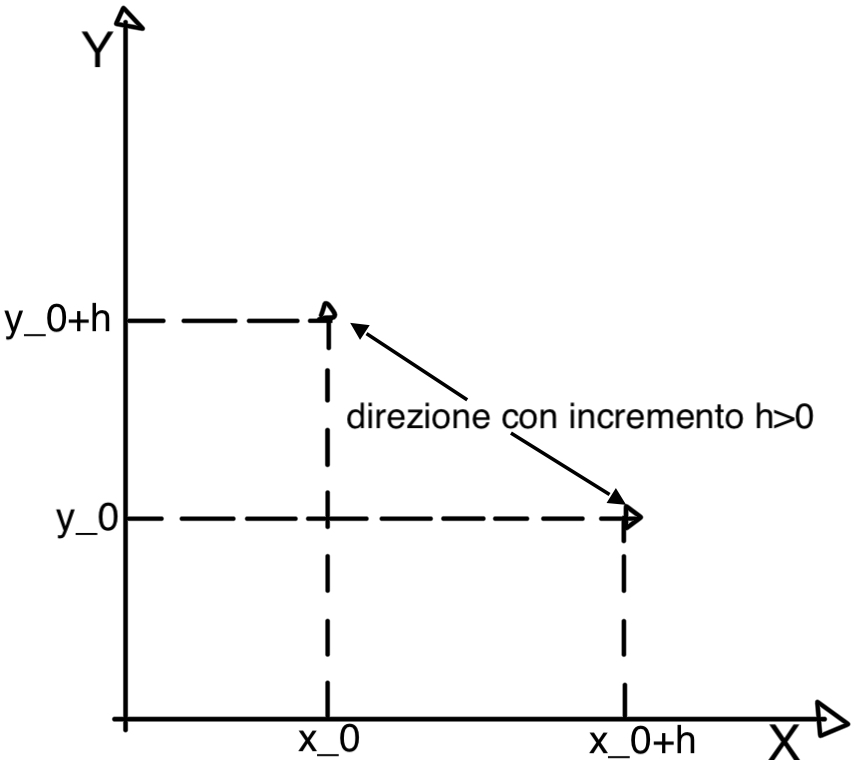
\includegraphics[width=0.65\textwidth]{Analisi2/figures/rappresentazione_direzione_R2.jpeg}
    \caption{Rappresentazione delle direzioni con incremento $h>0$.}\label{fig:rappresentazione_direzione_R2}
\end{figure}

\paragraph{N.B.:} \textbf{La Definizione \ref{def:derivata_parziale_Rn} di derivata parziale e la Definizione \ref{def:derivata_direzionale_Rn} di derivata direzionale sono equivalenti.}

\begin{definition}[Derivata parziale in $\mathbb R^n$]\label{def:derivata_parziale_Rn}\footnote{Slide 2 PDF 14.}
    Sia $f:A\subseteq\mathbb R^n\rightarrow\mathbb R$, con $A$ aperto e sia $P_0\overset{\footnotemark}{=}(x_1,x_2,\hdots, x_n)\in A$. La derivata parziale di $f$ rispetto alla variabile $x_i$ (dove $i=1,\hdots, n$) nel punto $P_0$ è data da
    \begin{equation}\label{eq:derivata_parziale_Rn}
        \lim_{h\rightarrow 0}\frac{f(x_1,\hdots,x_{i-1},x_i+h,x_{i+1},\hdots,  x_n)-f(x_1,\hdots, x_n)}{h}:=\frac{\partial f}{\partial x_i}(P_0)
    \end{equation}
    purché questo limite esista e sia finito.
\end{definition}
\footnotetext{Non è utilizzata la notazione $P_0=(x^0_1,x^0_2,\hdots, x^0_n)$ per appesantire la notazione della definizione.}

\paragraph{Quante sono le derivate parziali di una funzione di $n$ variabili?} Una funzione di $n$ variabili derivabile in un punto ha $n$ derivate parziali.

\paragraph{Perché è utilizzato sempre un aperto per le definizioni di derivate / gradiente e Teoremi affini?} Un insieme aperto ha la caratteristica topologica che ogni suo punto è interno. Per i tipi di insiemi considerati i domini sono della forma $D=A\cup\partial A$, quindi la parte interna di $D$ è un aperto. Queste proprietà sono utili perché è importante che dato un punto di un aperto allora le proprietà che saranno dimostrate nel punto valgano nell'intorno centrato nel punto.

\paragraph{Notazione per le derivate parziali:}
\begin{equation*}
    \frac{\partial f}{\partial x_i}(P_0)=f_{x_i}(P_0)=\frac{\partial f}{\partial x_i}(x_1,\hdots,x_n)=f_{x_i}(x_1,\hdots,x_n)=  D_{x_i}(P_0)=D_{x_i}(x_1,\hdots,x_n).
\end{equation*}

\begin{definition}[Derivabilità in $A$]\footnote{Slide 10 PDF 14.}
   Considerata $f:A\subseteq\mathbb R^n\rightarrow\mathbb R$. Se $f$ è derivabile in ogni punto $\uline x=(x_1,\hdots,x_n)\in A$, $f$ si dice derivabile in $A$ (ovvero esistono finite tutte le $n$ derivate parziali per ogni punto di $A$).
\end{definition}

In modo analogo al caso in due variabili, quando è calcolata la derivata parziale rispetto alla variabile $i$-esima, dove $i=1,\hdots,n$, sono tenute fisse tutte le variabili tranne la $i$-esima, la quale subisce un incremento. Considerando la $f$ in (\ref{eq:derivata_parziale_Rn}), sono tenute fisse tutte le variabili escluse la $i$-esima, sulla quale è applicato l'incremento. Quindi, il calcolo delle derivate parziali diventa un problema di Analisi 1 perché $f$ è come se fosse a una variabile, per il congelamento delle variabili.

Tornando alle funzioni in due variabili, le due derivate parziali sono (\ref{eq:derivata_parziale_x}) e (\ref{eq:derivata_parziale_y}), dove la funzione che subisce l'incremento in entrambi i limiti è ad una sola variabile (rispettivamente la $y$ e la $x$ sono fisse). Inoltre, quando sono state introdotte le sezioni (tracce) delle funzioni (vedere (\ref{eq:piani}) in Sezione \ref{ssec:grafico_funzione_n_variabili}) è stato spiegato che tenendo fissa una variabile è come se fatta l'intersezione della funzione con il piano e quindi è ottenuto il grafico di una funzione di una variabile. Quindi, quando sono date le derivate parziali (\ref{eq:derivata_parziale_x}) e (\ref{eq:derivata_parziale_y}) sono considerate le tracce della funzione lungo i piani $x=x_0$ o $y=y_0$ (come descritto in (\ref{eq:sezione_derivate_parziali})). Ad esempio: in (\ref{eq:derivata_parziale_x}) (ovvero $f_x(\uline x)$) è fissato $y=y_0$, quindi è come fare la traccia considerando l'intersezione della sezione con il piano $y=y_0$. Analogo fissato $x=x_0$ (ovvero con $f_y(\uline x)$).

\begin{equation}\label{eq:sezione_derivate_parziali}
    \begin{cases}
        z=graf\, f=f(x,y)\\
        x=x_0
    \end{cases}\rightarrow z=f(x_0,y)
    \quad\text{oppure}\quad
    \begin{cases}
        z=f(x,y)\\
        y=y_0
    \end{cases}\rightarrow z=f(x,y_0)
\end{equation}
dove $x_0$ o $y_0$ sono fissati e quindi $f$ diventa una funzione di una variabile.

Quindi con le sezioni del grafico ottenute tramite (\ref{eq:sezione_derivate_parziali}) sono ottenuti i grafici di curve di funzioni di una variabile nei rispettivi piani $(y,z)$ e $(x,z)$. Ciò significa che le derivate parziali delle funzioni di due variabili non sono altro che le derivate parziali, rispetto $x$ ed $y$, delle funzioni di una variabile, dove queste ultime sono le tracce della funzione in due variabili.

Infatti, se è considerata la traccia di $f(x,y)$ lungo il piano $y=y_0$ (è ottenuto)
\begin{equation*}
    f(x,y_0):=g_1(x). \footnotemark
\end{equation*}
\footnotetext{$y$ è fissa perché $y=y_0$. Quindi, come in Analisi 1, se $g_1$ è derivabile nel punto allora $g'(x)$ è la derivata parziale di $f$ rispetto ad $x$.}

Se $g_1$ è derivabile in $x_0$ significa che esiste ed è finito (il limite del rapporto incrementale di $g_1$ nel punto $x_0$, ovvero)
\begin{equation*}
    \lim_{h\rightarrow 0}\frac{g_1(x_0+h)+g_1(x_0)}{h}:=g'_1(x_0)=\frac{\partial f}{\partial x}(x_0,y_0).
\end{equation*}

Infatti
\begin{equation*}
    \lim_{h\rightarrow 0}\frac{g_1(x_0+h)+g_1(x_0)}{h}=\lim_{h\rightarrow 0}\frac{f(x_0+h,y_0)-f(x_0,y_0)}{h}.
\end{equation*}

Analogo risultato considerata la traccia di $f$ lungo il piano $x=x_0$, con
\begin{equation*}
    f(x_0,y):=g_2(y).
\end{equation*}

Se $g_2$ è derivabile in $y_0$ significa che esiste ed è finito (il limite del rapporto incrementale di $g_2$ nel punto $y_0$, ovvero)
\begin{equation*}
    \lim_{h\rightarrow 0}\frac{g_2(y_0+h)+g_2(y_0)}{h}:=g'_2(y_0)=\frac{\partial f}{\partial y}(x_0,y_0).
\end{equation*}

\paragraph{Quindi come sono calcolate le derivate?} Fissate tutte le variabili tranne l'$i$-esima è calcolato il limite del rapporto incrementale, oppure sono considerate le tracce (i due procedimenti sono simili).

\begin{example}[Calcolo di derivate parziali]\footnote{Slide 6 PDF 14.}
    Sia $f(x,y)=x\cos(x^2y^3)+x^6y^2+e^x$.
    \begin{equation}\label{eq:derivate_parziali_metodo_normale}
        \begin{matrix}
            \frac{\partial f}{\partial x}(x,y)&=& \cos(x^2y^3)-x\sin(x^2y^3)(2xy^3)+6x^5y^2+e^x&=&\cos(x^2y^3)-2x^2y^3\sin(x^2y^3)+6x^5y^2+e^x,\\\\
            \frac{\partial f}{\partial y}(P_0)&=& -x\sin(x^2y^3)(3x^2y^2)+2x^6y&=&-3x^3y^2\sin(x^2y^3)+2x^6y.
        \end{matrix}
    \end{equation}
    Calcoliamo tali derivate in $P_0=(1,2)$:
    \begin{equation*}
        \begin{matrix}
            \frac{\partial f}{\partial x}(P_0)&=& \cos(1\cdot 2^3)-2\cdot 1\cdot 2^3\sin(1\cdot 2^3)+6\cdot 1\cdot 2^2+e^1&=&\cos8 -16\sin8+24+ e,\\\\
            \frac{\partial f}{\partial y}(x,y)&=&-3\cdot 1^3\cdot 2^2\sin(1^2\,2^3)+2\cdot1^6\cdot2 &=&-12\sin8+4.
        \end{matrix}
    \end{equation*}
    \footnote{Tramite le tracce è possibile calcolare le derivate parziali nel punto $P_0$ ottenendo lo stesso risultato.}
    Utilizzando le tracce (sono fissate $x$ e $y$) $x=1$ e $y=2$, le  derivate sono calcolate come segue:\\
    (Lungo il piano $y=2$)
    \begin{equation*}
        \begin{matrix}
            f(x,2)&=&g_1(x)&\overset{\footnotemark}{=}&x\cos(8x^2)+4x^6+e^x,\\
            g'_1(x)&=&\cos(8x^2)&=&-x\sin(8x^2)16x+24x^5+e^x,\\
            g'_1(1)&=& f_x(1,2)&=& \cos(8)-16\sin8+24+e.
        \end{matrix}
    \end{equation*}
    \footnotetext{Traccia lungo il piano $y=2$. Quindi è calcolata la derivata della funzione di una variabile nel punto $x=1$ così da avere la derivata parziale rispetto ad $x$ calcolata nel punto $(1,2)$.} (Lungo il piano  $x=1$)
    \begin{equation*}
        \begin{matrix}
            f(1,y) &=& g_2(y) &=& \cos(x^2+y^2)+y^2+e\\
            g_2'(y) &=& -3y^2\sin(y^3)+2y\\
            g'_2(2) &=& -3\cdot 2^2\sin 8+ 4 &=& -12\sin 8+4.
        \end{matrix}
    \end{equation*}
    È possibile notare che le derivate parziali ottenute con i due procedimenti sono uguali.
\end{example}
\paragraph{N.B.:} Dall'esempio è possibile notare che il metodo delle tracce è più lungo del metodo utilizzando in (\ref{eq:derivate_parziali_metodo_normale}). La differenza tra i due metodi è che il (\ref{eq:derivate_parziali_metodo_normale}) presuppone che la derivata esista e se esiste è possibile calcolarla (é presupposto quindi che esista il limite del rapporto incrementale); il metodo delle tracce considera le funzioni secondo le due tracce e poi verifica che le funzioni di una variabile siano derivabili. Tuttavia, essendo $\sin,\, \cos$ e la seconda parte delle derivate funzioni regolari e appartenenti a $C^\infty$,  è naturale utilizzare il metodo (\ref{eq:derivate_parziali_metodo_normale}).

\begin{example}[Funzione derivabile ma non continua in un punto]\footnote{Slide 7 PDF 14.}
    Calcolare e esistono le derivate parziali nell'origine (ovvero in $P_0=(0,0)$) della seguente funzione:
    \begin{equation*}
        f(x,y)=
        \begin{cases}
            \frac{xy^2}{x^2+y^4} & \text{se } (x,y)\neq (0,0),\\
            0 & \text{se } (x,y)=(0,0).
        \end{cases}
    \end{equation*}
    $f:\mathbb R^2\rightarrow\mathbb R$.\\
    (Consideriamo le) tracce della funzione:
    \begin{equation*}
        \begin{matrix}
            f(x,0)=0=g_1(x),\\
            f(0,y)=0=g_2(y),
        \end{matrix}
    \end{equation*}
    e dunque (dato che $g_1$ e $g_2$ sono identicamente nulle, le derivate parziali sono)
    \begin{equation*}
        \frac{\partial f}{\partial x}(0,0)=\frac{\partial f}{\partial y}(0,0)=0.
    \end{equation*}
    Quindi $f$ è derivabile in $(0,0)$. \footnote{Dimostriamo che la funzione non è continua tramite la definizione di continuità nel punto, in particolare è mostrato (dopo la nota) che il limite di $f$ quando $(x,y)\rightarrow (0,0)$ non esiste. Per dimostrare la continuità è verificato il limite (\ref{eq:limite_continuita}) della Definizione \ref{def:continuita_funzione_n_variabili} di continuità.} Mostriamo che il limite $\lim_{(x,y)\rightarrow(0,0)}f(x,y)$ non esiste:
    \begin{equation*}
        \lim_{(x,y)\rightarrow(0,0)}\frac{xy^2}{x^2+y^4}.
    \end{equation*}
    Il candidato limite è 0 perché lungo gli assi $x=0$ e $y=0$ vale 0.\\
    Lungo l'asse $x=y^2$
    \begin{equation*}
        \underset{x=y^2}{\lim_{(x,y)\rightarrow(0,0)}}f(x,y)=\lim_{y\rightarrow 0}\frac{y^4}{y^4+y^4}=\frac{1}{2}\neq 0.
    \end{equation*}
    Dunque $f$ non è continua ma è derivabile in $(0,0)$.
\end{example}

\paragraph{N.B.:} Questo esempio aiuta a capire che se vogliamo estendere al caso in più variabili l'implicazione funzione derivabile $\rightarrow$ funzione continua, è necessario definire la differenziabilità.

\begin{definition}[Gradiente]\footnote{Slide 10 PDF 14.}
   Sia $f:A\subseteq\mathbb R^n\rightarrow\mathbb R$. Se $f$ è derivabile in $\uline x\in A$ esiste il vettore gradiente nel punto $\uline x$, il quale è definito come
   \begin{equation}
       \boldsymbol{\triangledown f(\uline x)=}\triangledown f(x_1,\hdots, x_n)=\boldsymbol{\left(\frac{\partial f}{\partial x_1}(\uline x),\hdots, \frac{\partial f}{\partial x_n}(\uline x)\right)^T}\in\mathbb R^n.
   \end{equation}
\end{definition}

\begin{example}[Gradiente in $\mathbb R^2$]\footnote{Slide 10 PDF 14.}
    Sia $f:A\subseteq\mathbb R^2\rightarrow\mathbb R$ e $P_0=(x_0,y_0)\in A$. Se $f$ è derivabile in $P_0$ allora esistono finite
    \begin{equation*}
        \frac{\partial f}{\partial x}(P_0),\; \frac{\partial f}{\partial y}(P_0),
    \end{equation*}
    quindi esiste
    \begin{equation*}
        \triangledown f(P_0)=\left(\frac{\partial f}{\partial x}(P_0),\frac{\partial f}{\partial y}(P_0)\right)=\frac{\partial f}{\partial x}(P_0)\; \uline i+ \frac{\partial f}{\partial y}(P_0)\; \uline j.
    \end{equation*}
\end{example}

\subsubsection{Significato geometrico delle derivate parziali}
\footnote{Slide 11 PDF 14.}Per dare un senso geometrico alle derivate parziali sono considerate le funzioni di 2 variabili perché è possibile disegnarne il grafico (per funzioni di $n>2$ variabili non è possibile).

\paragraph{Per le funzioni in una variabile} $f'(x_0)\in\mathbb R$ è il coefficiente angolare (la pendenza) della retta tangente al grafico di $f$ $y-t_0=f'(x_0)(x-x_0)$ per $P_0=(x_0,f(x_0))\in graf\, f\subset \mathbb R^2$.

\paragraph{Per le funzioni in due variabili} le derivate parziali sono legate rette tangenti al grafico delle curve ottenute nei piani corrispondenti fissate le tracce. Questo perché le derivate parziali sono calcolate fissate le tracce $x=x_0$ oppure $y=y_0$, come in (\ref{eq:traccia_derivata_parziale_y}) ed in (\ref{eq:traccia_derivata_parziale_x}).

(Traccia nel piano $(y,z)$)
\begin{equation}\label{eq:traccia_derivata_parziale_y}
    \begin{cases}
        x=x_0\\
        z\overset{\footnotemark}{=}f(x_0,y)
    \end{cases}
\end{equation}
\footnotetext{$f$ dipende da $y$.}

(Traccia nel piano $(x,z)$)
\begin{equation}\label{eq:traccia_derivata_parziale_x}
    \begin{cases}
        y=y_0\\
        z=f(x,y_0)
    \end{cases}
\end{equation}

\paragraph{N.B.:} Una curva è da intendersi come traiettoria (vedere la Sezione \ref{ssec:curve_Rn} nella quale sono trattate le curve).

\subsubsection{Piano tangente}
\paragraph{Osservazioni su Figura \ref{fig:grafico_f_R3_osservazione}:}\footnote{Slide 12-13 PDF 14.}
Sia $f\colon A\subseteq\mathbb R^2\rightarrow\mathbb R$, con $A$ aperto. Il grafico di $f$ $graf\,f=\{(x,y,z)\in\mathbb R^3\,|\, z=f(x,y),\, \forall (x,y)\in A\}\subset\mathbb R^3$ è un sottoinsieme dello spazio vettoriale $\mathbb R^3$ ed è una superficie in tale spazio. È una superficie perché stiamo lavorando sugli aperti e sulla regolarità della funzione.\\
Considerando $P_0=(x_0,y_0,z_0)\in graf\, f$, dove $z_0=f(x_0,y_0)$ vedere Figura \ref{fig:grafico_f_R3_osservazione}.\\
Quando sono calcolate le derivate parziali sono considerate le tracce $y=y_0$ e $x=x_0$ per avere rispettivamente le derivate parziali rispetto $x$ e $y$. Quindi, quando è considerata una traccia è intersecato il grafico di $f$ con $y=y_0$ o $x=x_0$, ovvero: taglio il grafico con $y=y_0$ per ottenere la sezione del grafico nel piano $(x,y)$, analogo per $x=x_0$.\\
Considerando la traccia lungo $y=y_0$ allora
\begin{equation}\label{eq:traccia_g_1}
    \begin{cases}
        z=f(x,y)=f(x,y_0)=g_1(x)\\
        y=y_0\quad \text{piano }(x,z)
    \end{cases}
\end{equation}
Il grafico di $g_1(x)$ è nel piano $(x,z)$ ed è rappresentato dalla curva $c_1$ in Figura \ref{fig:grafico_f_R3_osservazione}. Quanto in (\ref{eq:traccia_g_1}) può essere descritto come segue: $c_1$ è il grafico della curva $g_1(x)=f(x,y_0)=z$ piano $(x,z)$ passante per $P_0$ ottenuta tagliando il grafico di $f$ con $y=y_0$ ed è immaginabile come traiettoria nel piano corrispondente ottenuta dalla sezione. Ovvero, $c_1$ è l'intersezione del grafico di $f$ ($graf\, f\subset\mathbb R^3$) con il piano $(x,z)$. Inoltre, per la curva $c_1$, $g_1'(x)=\frac{\partial f}{\partial x}(x_0,y_0)$ è il coefficiente angolare di $c_1$ in $x_0$ e il coefficiente angolare della retta $T_1$ (ovvero la retta tangente al grafico della funzione $c_1$).\\
Un ragionamento analogo lungo il piano $x=x_0$.\\
 $T_1$ e $T_2$ sono rispettivamente le tangenti alle curve $c_1$ e $c_2$ con rispettivi coefficienti angolari $g'_1(x_0)$ e $g_2'(x_0)$. $T_1$ e $T_2$ hanno un unico punto in comune e per esse passa un unico piano passante per il punto $P_0$. È necessario ricordare che ci sono tante rette tangenti.\\
In Figura \ref{fig:grafico_f_R3_osservazione} $(x_0,y_0,0)$ è il punto sul piano $(x,y)$ di quota $z=z_0=0$ e fa parte dell'insieme di livello con $z=z_0=0$, quindi è un sottoinsieme del dominio $A$. $P_0=(x_0,y_0,z_0)$, con $z_0=f(x_0,y_0)$ è "tirato su" da $(x_0,y_0,0)$ ed è il punto $(x_0,y_0)$ di quota $z_0$. [Fine Osservazioni su Figura \ref{fig:grafico_f_R3_osservazione}]$\qed$
\begin{figure}[ht]
    \centering
    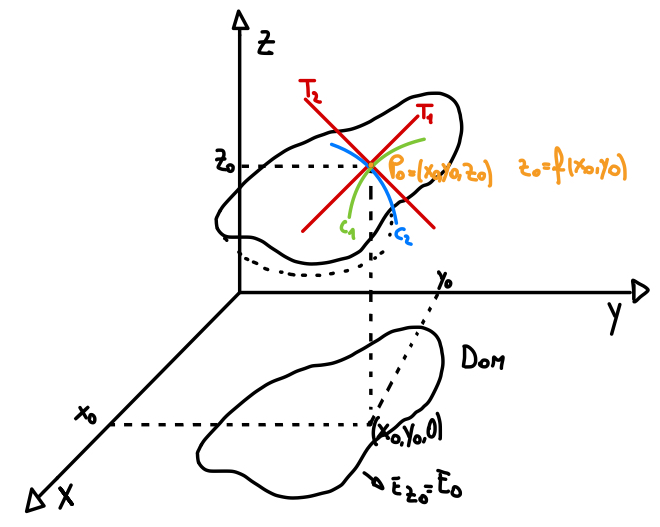
\includegraphics[width=0.65\textwidth]{Analisi2/figures/grafico_f_R3_osservazione.png}
    \caption{Grafico con rette tangenti.}\label{fig:grafico_f_R3_osservazione}
\end{figure}

\subsubsection{Curve in \texorpdfstring{$\boldsymbol{\mathbb R^n}$}{Rn}}\label{ssec:curve_Rn}\footnote{Slide 5 PDF 15.}
In matematica le curve sono delle applicazioni continue definite da un intervallo ad $\mathbb R^n$. In particolare, le curve piane sono delle applicazioni da un intervallo ad $\mathbb R^2$. Inoltre, il sostegno di una curva è l'immagine di una curva.

\subsubsection{Differenziabilità}
La derivabilità di una funzione di più variabili non implica la sua continuità. Il concetto necessario da introdurre per un tipo di implicazione del genere è quello di differenziabilità (vedere Definizione (\ref{def:differenziabilita_funzione_piu_variabili})). Per le funzioni di più variabili la differenziabilità è una proprietà più forte della derivabilità perché richiede che la funzione sia derivabile e che abbia alcune proprietà legate all'approssimazione lineare ottenuta per una funzione di una variabile con l'utilizzo della derivata prima (retta tangente).

Vedere il Teorema (\ref{th:del_differenziale}) del differenziale per capire che la differenziabilità è una proprietà più forte della derivabilità.

\subsubsection{Derivate Successive}

\section{Calcolo integrale per funzioni di più variabili (secondo Riemann)}


\section{Fogli Esercizi}

\subsection{EDOI-INFORMATICA}
\begin{enumerate}
    \item Determinare l'integrale generale dell'equazione
    \begin{equation*}
        ye^{2t}-(1+e^{2t})y'=0.
    \end{equation*}
    \item Determinare l'integrale generale delle equazioni
    \begin{enumerate}
        \item $(1+t^2)y'+ty=(1+t^2)^{-1}$,
        \item $y'=\frac{2xy}{x^2-1}$.
    \end{enumerate}
\end{enumerate}

\paragraph{1.}

\paragraph{2.1} Dato $(1+t^2)y'+ty=(1+t^2)^{-1}$, allora dividendo per $(1+t^2)$
\begin{equation*}
    y'+\frac{t}{1+t^2}y=(1+t^2)^{-2}.
\end{equation*}
\begin{equation*}
    \int a(x)\, dx=\int \frac{t}{1+t^2}\, dt = \frac{1}{2}\log(1+t^2),
\end{equation*}
quindi,
\begin{equation*}
    z(x)=c\cdot\frac{1}{\sqrt{1+t^2}}.
\end{equation*}
L'integrale generale ricercato è
\begin{equation*}
    \boldsymbol{y(x)=}c\frac{1}{\sqrt{1+t^2}}+\frac{1}{\sqrt{1+t^2}}\int\frac{\sqrt{1+t^2}}{(1+t^2)^2}\, dx\overset{\footnotemark}{=} c\frac{1}{\sqrt{1+t^2}}+\frac{1}{\sqrt{1+t^2}}\cdot\frac{x}{\sqrt{1+t^2}}= \boldsymbol{c\frac{1}{\sqrt{1+t^2}}+\frac{x}{\sqrt{1+t^2}}.}
\end{equation*}
\footnotetext{Integrale risolto per sostituzione: con $x=\tan u,\, dx=\frac{1}{\cos^2(u)}\, du$, $\int\frac{\sqrt{1+t^2}}{(1+t^2)^2}\, dx=$.}

\end{document}